%\documentclass{book}
%
%\usepackage{fancyhdr}
%\usepackage{extramarks}
%\usepackage{amsmath}
%\usepackage{esint}
%\usepackage{amsthm}
%\usepackage{amsfonts}
%\usepackage{tikz}
%\usepackage{enumerate}
%\usepackage{graphicx}
%\graphicspath{ {images/} }
%\usepackage[plain]{algorithm}
%\usepackage{algpseudocode}
%\usepackage[document]{ragged2e}
%\usepackage{textcomp}
%\usepackage{color}   %May be necessary if you want to color links
%\usepackage{import}
%\usepackage{natbib}
%\usepackage{hyperref}
%\hypersetup{
%    colorlinks=true, %set true if you want colored links
%    linktoc=all,     %set to all if you want both sections and subsections linked
%    linkcolor=black,  %choose some color if you want links to stand out
%}
%
%\usetikzlibrary{automata,positioning}
%
%
%% Basic Document Settings
%
%
%\topmargin=-0.45in
%\evensidemargin=0in
%\oddsidemargin=0in
%\textwidth=6.5in
%\textheight=9.0in
%\headsep=0.25in
%\setlength{\parskip}{1em}
%
%\linespread{1.1}
%
%\pagestyle{fancy}
%\lhead{\hmwkAuthorName}
%\lfoot{\lastxmark}
%\cfoot{\thepage}
%
%\renewcommand\headrulewidth{0.4pt}
%\renewcommand\footrulewidth{0.4pt}
%
%\setlength\parindent{0pt}
%
%
%\newcommand{\hmwkTitle}{Math Review Notes---Real Analysis}
%\newcommand{\hmwkAuthorName}{\textbf{G. Faletto} }
%
%
%%%%%% Title Page
%
%
%\title{
%    \vspace{2in}
%    \textmd{\textbf{ \hmwkTitle}}\\
%}
%
%\author{Gregory Faletto}
%\date{}
%
%\renewcommand{\part}[1]{\textbf{\large Part \Alph{partCounter}}\stepcounter{partCounter}\\}
%
%
%%%%%% Various Helper Commands
%
%
%%%%%% Useful for algorithms
%\newcommand{\alg}[1]{\textsc{\bfseries \footnotesize #1}}
%
%%%%%% For derivatives
%\newcommand{\deriv}[2]{\frac{\mathrm{d} #1}{\mathrm{d} #2}}
%
%%%%%% For partial derivatives
%\newcommand{\pderiv}[2]{\frac{\partial #1}{\partial #2}}
%
%%%%%% Integral dx
%\newcommand{\dx}{\mathrm{d}x}
%
%%%%%% Alias for the Solution section header
%\newcommand{\solution}{\textbf{\large Solution}}
%
%%%%%% Probability commands: Expectation, Variance, Covariance, Bias
%\newcommand{\E}{\mathbb{E}}
%\newcommand{\Var}{\mathrm{Var}}
%\newcommand{\Cov}{\mathrm{Cov}}
%\newcommand{\Bias}{\mathrm{Bias}}
%\newcommand\indep{\protect\mathpalette{\protect\independenT}{\perp}}
%\def\independenT#1#2{\mathrel{\rlap{$#1#2$}\mkern2mu{#1#2}}}
%\DeclareMathOperator{\Tr}{Tr}
%
%\theoremstyle{definition}
%\newtheorem{theorem}{Theorem}
%\theoremstyle{definition}
%\newtheorem{proposition}[theorem]{Proposition}
%\theoremstyle{definition}
%\newtheorem{lemma}[theorem]{Lemma}
%\theoremstyle{definition}
%\newtheorem{corollary}{Corollary}[theorem]
%\theoremstyle{definition}
%\newtheorem{definition}{Definition}[section]
%\newtheorem{remark}{Remark}
%\theoremstyle{definition}
%\newtheorem{exercise}{Exercise}
%\theoremstyle{definition}
%\newtheorem{example}{Example}[section]
%
%%%%%% Tilde
%\newcommand{\textapprox}{\raisebox{0.5ex}{\texttildelow}}
%
%\begin{document}
%
%\maketitle
%
%\pagebreak
%
%\tableofcontents
%
%\
%
%\
%
%\begin{center}
%Last updated \today
%\end{center}
%
%
%
%\newpage
%
%%
%%
%%
%%
%%
%%
%%
%%
%%%
%% Real Analysis

% Real Analysis
\chapter{Real Analysis}

These are my notes from Math 4650: Analysis I at Cal State LA, Math 425B: Fundamental Concepts of Analysis at USC taught by Andrew Manion and the textbook \citep{pugh2015real}, the textbook \citep{rudin1976principles}, as well as Prof. Steven Heilman's notes from Math 541A at USC.

%\textbf{Brush up on recent real analysis (especially open, closed, compact, etc)}

%Midterm 1
\section{Midterm 1}

% Homework 1
\subsection{Homework 1}

\begin{definition} Let \(S \subseteq \mathbb{R}\). We say that \(S\) is \textbf{bounded from above} if \(\exists \ b \in \mathbb{R}\) where \[s \leq b \ \forall \ s \in S\]If this is the case, we call \(b\) an \textbf{upper bound} of \(S\).

If \(b \leq c \) for all upper bounds \(c\) of \(S\), we call \(b\) the \textbf{supremum} of \(S\): \(b = \sup(S)\).

\end{definition}

\begin{definition} We say that \(S\) is \textbf{bounded from below} if \(\exists \ a \in \mathbb{R}\) where \[s \geq a \ \forall \ s \in S\]If this is the case, we call \(a\) a \textbf{lower bound} of \(S\).

If \(a \geq d \) for all lower bounds \(d\) of \(S\), we call \(a\) the \textbf{infimum} of \(S\): \(a = \inf(S)\).
\end{definition}

\begin{proposition} \textbf{Useful Sup/Inf Fact:} Let \(S \in \mathbb{R}\), \(S \neq \emptyset\). 

\begin{enumerate}[(1)]

\item Suppose \(S\) is bounded from above by an element \(b\). Then \(b = \sup(S) \iff \forall \ \epsilon >0 \ \exists \ x \in S\) with \[b - \epsilon < x \leq b\]

\item Suppose \(S\) is bounded from below by an element \(a\). Then \(a = \inf(S) \iff \forall \ \epsilon >0 \ \exists \ x \in S\) with \[a \leq x < a + \epsilon\]

\end{enumerate}

\end{proposition}

\textbf{Completeness Axiom}: Let \(S\) be a nonempty subset of \(\mathbb{R}\). If \(S\) is bounded from above, then \(\sup(S)\) exists. If \(S\) is bounded from below, then \(\inf(S)\) exists.

%\[
%|x - y| < \epsilon \iff y - \epsilon < x < y + \epsilon
%\]

\textbf{Facts about absolute value:}

\begin{itemize}

\item \begin{proposition}\label{ra.abs.fact1} \(|x-y| < \epsilon \iff y - \epsilon < x < y + \epsilon.\) \end{proposition}

\begin{proof}In notes 08/23.\end{proof}

\item \begin{proposition} \( |ab| = |a||b|. \)\end{proposition}

\begin{proof} \[| ab | = \begin{cases} 
      ab & ab \geq 0 \\
      -ab & ab < 0 
   \end{cases} = \begin{cases} 
      ab & a \geq 0,  b \geq 0 \\
      -ab & a \geq 0, b < 0 \\ 
      -ab & a < 0, b \geq 0 \\ 
      ab & a < 0,  b < 0 \\
   \end{cases} = \begin{cases} 
      ab & a \geq 0,  b \geq 0 \\
      a(-b) & a \geq 0, b < 0 \\ 
      (-a)b & a < 0, b \geq 0 \\ 
      (-a)(-b) & a < 0,  b < 0 \\
   \end{cases}
\]


\[= \begin{cases} 
      |a||b| & a \geq 0,  b \geq 0 \\
      |a||b| & a \geq 0, b < 0 \\ 
      |a||b| & a < 0, b \geq 0 \\ 
      |a||b| & a < 0,  b < 0 \\
   \end{cases} \implies | ab | = |a||b| 
\]

\end{proof}

\item \begin{proposition} Let \(\epsilon >0\). Then \(|a| < \epsilon \iff -\epsilon < a < \epsilon\). \end{proposition}

\begin{proof} Follows from Proposition \ref{ra.abs.fact1} if \(x = a\), \(y = 0\). \end{proof}

\item \begin{proposition} \(-|a| \leq a \leq |a|\)  \end{proposition}

\begin{proof}  Follows from Proposition \ref{ra.abs.fact1} if \(x = a\), \(y = 0\), \(\epsilon = |a|\). \end{proof}

\item \begin{theorem}\label{ra.tri.ineq.1} \textbf{Triangle Inequality:} \(|a + b| \leq |a| + |b|\). \end{theorem}

\begin{proof} In notes 08/23.\end{proof}

 \begin{corollary}\label{ra.tri.ineq.2} \textbf{Triangle Inequality:} \(|a - b| \leq |a| + |b|\). \end{corollary}

\begin{proof} Follows from Theorem \ref{ra.tri.ineq.1}, let \(b = -b\).

\end{proof}

\begin{remark} See also Theorem \ref{asym.tri.ineq.norm}.\end{remark}

\item \begin{proposition} \(|\ |a| - |b| \ | \leq |a - b|\). \end{proposition}

\begin{proof} By Proposition \ref{ra.abs.fact1}, \(|\ |a| - |b| \ | \leq |a - b|\) if and only if

\begin{equation}\label{ra.proof.eqn1}
|b| - |a - b| \leq |a| \leq |b| + |a - b|
\end{equation}

The left half of (\ref{ra.proof.eqn1}) is true by the Triangle Inequality (Theorem \ref{ra.tri.ineq.1}):

\[
|b| = |a - (a - b)| \leq |a| +  |a - b| \iff |b| \leq |a| +  |a - b| \iff  |b| - |a - b| \leq |a|
\]

The right half of  (\ref{ra.proof.eqn1}) is also true by the Triangle Inequality (Theorem \ref{ra.tri.ineq.1}):

\[
|a| = |b + a - b| \leq |b| + |a - b|
\]

Therefore

\[
|\ |a| - |b| \ | \leq |a - b|.
\] \end{proof}

\begin{proof}(Alternative proof.) Note that by the Triangle Inequality (Theorem \ref{ra.tri.ineq.1}),

\[
|a| = |a - b +b| \leq |a - b| + |b| \implies |a| - |b| \leq |a - b|
\]

Also,

\[
|b| = |b - a + a| \leq |b - a| + |a| \implies -|b - a| \leq |a| - |b| \implies -|a - b| \leq |a| - |b|
\]

where the last step follows from Proposition \ref{ra.abs.fact.a}. Therefore

\[
-|a - b| \leq |a| - |b| \leq |a - b|
\]

and by Proposition \ref{ra.abs.fact1},

\[
|\ |a| - |b| \ | \leq |a - b|.
\]
\end{proof}

\item \begin{proposition} If \(a < x < b\) and \(a < y < b\) then \(|x - y| < b - a\). \end{proposition}

\begin{proof}
\[
y > a \implies -y < -a \implies b - y < b - a
\]

\[
b > y \implies b - y = |b - y| \implies  \boxed{|b - y| < b - a}
\]

By the Triangle Inequality (Theorem \ref{ra.tri.ineq.1}),

\[
|x - y| = |x - b + b - y| \leq |x -b| + |b - y|
\]

Since \(b <x\), \(|x - b| > 0\). Therefore \(\boxed{|x - y| < | b - y|}\).

\[
\implies |x - y| < |b - y| < b - a
\]

\[
\implies |x - y| < b - a
\]
\end{proof}

\begin{proof} (Alternative proof.) Break into two cases.

\begin{itemize}

\item \textbf{Case 1:} \(x \geq y\). Then \(|x - y| = x - y\). We know \(a < x < b \implies 0 < x - a < b - a\). 

\[
a < y \implies -a > -y \implies x - a > x -y \implies x - y < x - a < b - a
\]

\[
\implies \boxed{|x - y| < b - a}
\]


\item \textbf{Case 2:} \(x < y\). Then \(|x - y| = y - x\). We know \(a < y < b \implies 0 < y - a < b - a\).

\[
a < x \implies -a > -x \implies y - a > y - x \implies y - x < y - a < b - a
\]

\[
\implies \boxed{|x - y| < b - a}
\]

\end{itemize}

\end{proof}

\item \begin{proposition}\label{ra.abs.fact.a} \(|a - b| = |b - a|\) \end{proposition}

\begin{proof} \(|a - b| = |(-1)(b - a)| = |-1||b-a| = |b - a|\), where the second-to-last step follows from Proposition \ref{ra.abs.fact1}.

\end{proof}

\end{itemize}

% Homework 2
\subsection{Homework 2}

\begin{definition}  A sequence \((a_n)\) of real numbers is said to \textbf{converge} to a \textbf{limit} \(L \in \mathbb{R}\) if \(\forall \ \epsilon > 0 \ \exists \ N > 0 \) where

\[
n \geq N \implies |a_n - L| < \epsilon
\]

We say that \((a_n)\) \textbf{diverges} if it does not converge.

\end{definition}

\begin{definition} A sequence \((a_n)\) of real numbers is \textbf{bounded} if \(\exists \ M > 0\) where \(\forall \ n \in \mathbb{N}\) \[\ |a_n| \leq M .\]

\end{definition}

\begin{theorem} If \((a_n)\) converges then \((a_n)\) is bounded. \end{theorem}

\begin{definition} Let \((a_n)\) be a sequence of real numbers. We say that \((a_n)\) is a \textbf{Cauchy sequence} if \(\forall \ \epsilon > 0 \ \exists \ N\) where

\[
n, m \geq N \implies |a_n - a_m| < \epsilon
\]

\end{definition}

\begin{theorem} \((a_n)\) is Cauchy if and only if \((a_n)\) converges.

\end{theorem}

\begin{corollary} If \((a_n)\) is Cauchy then \((a_n)\) is bounded.

\end{corollary}

%\begin{theorem} Suppose that \(\{a_n\}\) is a Cauchy sequence. Then \(\{a_n\}\) is bounded. \end{theorem}

\begin{proof} Let \(\epsilon = 1\). Since \((a_n)\) is Cauchy, \(\exists \ N > 0 \ | \ n, m \geq N \implies \)

\[
|a_n - a_m| < 1
\]

So, \(n \geq N \implies\)

\[
|a_n - a_N| < 1 \iff a_N - 1 < a_n < a_N + 1 \implies |a_n| < |a_N + 1| \leq |a_N| + 1
\]

Let \(M = \max \{ |a_1|, |a_2|, \ldots, |a_{N-1}|, |a_N| + 1\} \). Then \(|a_n| \leq  M \ \forall \ n \geq 1 \). Therefore \((a_n)\) is bounded.

\end{proof}

%\end{theorem}

\begin{theorem} \textbf{(Squeeze theorem.)} Suppose that \(\{a_n\}, \{b_n\},\) and \(\{c_n\}\) are sequences of real numbers such that \(a_n \leq b_n \leq c_n\) for all \(n\). If both \(\{a_n\}\) and \(\{c_n\}\) converge to \(L\), then \(\{b_n\}\) converges to \(L\).

\end{theorem}

\begin{proof} Let \(\epsilon >0\). \((a_n)\) converges to \(L \implies\)

\[
\forall \ \epsilon> 0 \ \exists \ N_A \ | \ n \geq N_A \implies | a_n - L | < \epsilon 
\]

\((c_n)\) converges to \(L \implies\)

\[
\forall \ \epsilon> 0 \ \exists \ N_C \ | \ n \geq N_C \implies | c_n - L | < \epsilon 
\]

Let \(N = \max \{N_A, N_C\} \). Then by one of our absolute values rules, \(n \geq N \implies\)

\[
| a_n - L | < \epsilon \iff L - \epsilon < a_n < L + \epsilon
\]

\[
| c_n - L | < \epsilon \iff L - \epsilon < c_n < L + \epsilon
\]

Therefore since \(a_n \leq b_n \leq c_n\),

\[
 L - \epsilon < a_n \leq b_n \leq c_n < L + \epsilon \implies L - \epsilon < b_n < L + \epsilon \iff | b_n - L | < \epsilon
\]

Therefore \((b_n)\) converges to \(L\).

\end{proof}

\begin{proposition} 
Limits of sequences in $\mathbb{R}$ are unique: if $a_n: \mathbb{N} \to \mathbb{R}$ is a sequence, $\lim a_n = L$, and $\lim a_n = L'$, then $L = L'$. 
\end{proposition}

\begin{proof}
Let \(L, L' \in \mathbb{R}\), with \(\lim_{n \to \infty} a_n = L\) and \(\lim_{n \to \infty} a_n = L'\). Then for all \(\epsilon > 0\) there exists \(N \in \mathbb{N}\) such that for all \(n \geq N\) we have \(|a_n - L| < \epsilon\), and there exists \(N' \in \mathbb{N}\) such that for all \(n \geq N'\) we have \(|a_n - L'| < \epsilon\). Suppose \(L \neq L'\), and let \(\epsilon := \frac{1}{2}|L - L'|  > 0\). But then for all \(n \geq \max\{N, N'\}\),

\[
2 \epsilon = |L - L'| = |L - a_n + a_n - L'|  \leq |a_n - L| + |a_n - L'| < \epsilon + \epsilon = 2 \epsilon,
\]

contradiction. Therefore \(L = L'\).

\end{proof}

\begin{theorem} Suppose that \(\{a_n\}\) and \(\{b_n\}\) are sequences of real numbers such that \(a_n \leq b_n\) for all \(n\). If \(\{a_n\}\) and \(\{b_n\}\) converge to \(A\) and \(B\) respectively, then \(A \leq B\).

\end{theorem}

\begin{proof} Suppose \(A > B\). Then let \(\epsilon = \frac{A - B}{4} > 0\). \((a_n)\) converges to \(A \implies\)

\[
\exists \ N_A \ | \ n \geq N_A \implies | a_n - A | < \epsilon \iff A - \epsilon < a_n < A + \epsilon
\]

\((b_n)\) converges to \(B \implies\)

\[
\exists \ N_B \ | \ n \geq N_B \implies | b_n - B | < \epsilon \iff B - \epsilon < b_n < B + \epsilon
\]

Then if \(n > \max \{ N_A, N_B\} \),

\[
A - \epsilon < a_n < A + \epsilon \iff A - \frac{A - B}{4} < a_n < A +\frac{A - B}{4} \iff \frac{3A}{4} + \frac{B}{4} < a_n <  \frac{5A}{4} - \frac{B}{4}
\]

\[
B - \epsilon < b_n < B + \epsilon \iff B -\frac{A - B}{4}< b_n < B+ \frac{A - B}{4} \iff \frac{5B}{4} - \frac{A}{4} < b_n <  \frac{3B}{4} + \frac{A}{4}
\]

This implies

\[
 b_n <  \frac{3B}{4} + \frac{A}{4} = \frac{B}{4} + \frac{A}{4} + \frac{2B}{4} < \frac{B}{4} + \frac{A}{4} + \frac{2A}{4}  = \frac{3A}{4} + \frac{B}{4} < a_n
\]

Contradiction, since it is given that \(a_n \leq b_n \ \forall \ n\). Therefore \(A \leq B\).
\end{proof}

\pagebreak

% Midterm 2
\section{Midterm 2}

% Homework 3
\subsection{Homework 3}

\begin{definition} \textbf{(Limits of functions at infinity.)} Let \(f\) be a real-valued function defined on some set \(D\) where \(D\) contains an interval of the form \((a, \infty)\). Let \(L \in \mathbb{R}\). We say \[\lim_{x \to \infty} f(x) = L\]if \(\forall \ \epsilon >0 \ \exists \ N \in \mathbb{R}\) where

\[
x \geq N \implies |f(x) - L| < \epsilon.
\]

\end{definition}

\begin{definition}\label{ra.def.limit.point} Let \(D \subseteq \mathbb{R}\). Let \(a \in \mathbb{R}\). We say that \(a\) is a \textbf{limit point} (or ``cluster point," or ``accumulation point") of \(D\) if \(\forall \ \delta > 0 \ \exists \ x \in D\) where

\[
x \neq a \text{ and } |x - a| < \delta
\]

(Note that \(a\) may or may not be contained in \(D\).)

\end{definition}

\begin{definition} \textbf{(Limit of a function at \(a\).)}: Let \(D \subseteq \mathbb{R}\) and \(f:d \to \mathbb{R}\). Let \(a\) be a limit point of \(D\). Let \(x \in D\). We say that \(f\) has a \textit{limit as \(x\) tends to \(a\)} if \(\exists \ L \in \mathbb{R}\) where \(\forall \ \epsilon > 0 \ \exists \ \delta > 0 \) such that

\[
0 < |x - a| < \delta \implies |f(x) - L| < \epsilon
\]

and we write \[\lim_{x \to a} f(x) = L\]

\end{definition}

\begin{proposition} \textbf{(Properties of Limits.)} Let \(D \in \mathbb{R}\) and let \(a\) be a limit point of \(D\). Suppose \(f:D \to \mathbb{R}\) and \(g: D \to \mathbb{R}\). Let \(\alpha \in \mathbb{R}\).

\begin{enumerate}[(1)]

\item If \(\lim_{x \to a} f(x) = L\) and \(\lim_{x \to a} g(x) = M\) then

\begin{enumerate}[(a)]

\item \[\lim_{x \to a} \alpha = \alpha\]

\item \[\lim_{x \to a} [f(x) + g(x)] = L + M\]

\item \[\lim_{x \to a} [f(x) - g(x)] = L - M\]

\item \[\lim_{x \to a} [f(x) \cdot g(x)] = L \cdot M\]

\item \[\lim_{x \to a} [\alpha \cdot f(x)] = \alpha \cdot L\]

\end{enumerate}

\item If \(h:D \to \mathbb{R}\) and \(h(x) \neq 0 \ \forall \ x \in D\) and \(\lim_{x \to a} h(x) = H \neq 0\), then

\[
\lim_{x \to a} \frac{1}{h(x)} = \frac{1}{H}
\]

Note that properties (2) and (1)(d) combined imply

\[
\lim_{x \to a} \frac{f(x)}{h(x)} = \frac{L}{H}
\]

\end{enumerate}

\end{proposition}

% Homework 4
\subsection{Homework 4}

\begin{definition} \textbf{(Continuity.)} Let \(D \subseteq \mathbb{R}\) and \(f:D \to \mathbb{R}\) and \(a \in D\). Then \(f\) is \textbf{continuous} at \(a\) if \(\lim_{x \to a} f(x)\) exists and 

\[
\lim_{x \to a} f(x) = f(a)
\]

\end{definition}

\begin{remark} if \(f\) is continuous at \(a\), then we can say \(\forall \ \epsilon > 0 \ \exists \ \delta > 0 \) such that

\[
|x - a| < \delta \implies |f(x) - L| < \epsilon
\]

that is, we don't need to say \(0 < |x - a| < \delta\).

\end{remark}

\begin{definition} If \(B \subseteq D\), then \(f\) is \textbf{continuous on B} if \(f\) is continuous at every \(b \in B\).

\end{definition}

\begin{theorem} \textbf{(Intermediate Value Theorem.)} Let \(f\) be continuous on \([a, b]\) and suppose \(f(a) < f(b)\). \(\forall \ d\) such that \[f(a) < d < f(b)\]  \(\exists \ c \in \mathbb{R}\) where \[a < c < b, \ f(c) = d.\]

\end{theorem}




%
%
%
%
%
%
%
%
%

\section{Real Numbers (Chapter 1 of \citet{pugh2015real}; also from Homework 6 of Math 4650 at Cal State LA)}

\begin{definition} \textbf{(Uniform Continuity (from Math 4650).)} Let \(D \subseteq \mathbb{R}\) and let \(f: D \to \mathbb{R}\). We say that \(f\) is \textbf{uniformly continuous} on \(D\) if \(\forall \ \epsilon > 0 \ \exists \ \delta > 0\) where

\[
x, y \in D \text{ and } 0 < |x - y| < \delta \implies |f(x) - f(y)| < \epsilon
\]

\end{definition}

\begin{theorem} \textbf{(Uniform continuity implies continuity; from Math 4650.)} Suppose \(f:D \to \mathbb{R}\) where \(D \subseteq \mathbb{R}\). If \(f\) is uniformly continuous on \(D\), then \(f\) is continuous at every \(a \in D\).

\end{theorem}

\begin{theorem}[\textbf{Theorem 2.42 in \citet{pugh2015real}}]

Every continuous function defined on a compact set is uniformly continuous.

\end{theorem}

\begin{definition}\label{ra.def.equiv}

Let \(S\) be any set, and let \(s, s', s'' \in S\). An \textbf{equivalence relation} on \(S\) is a relation \(s \sim s'\) that holds between some members \(s, s' \in S\) and satisfies three properties:

\begin{enumerate}[(a)]

\item \(s \sim s\)

\item \(s \sim s'\) implies \(s' \sim s\).

\item \(s \sim s'\) and \(s' \sim s''\) implies that \(s \sim s''\).

\end{enumerate}

An \textbf{equivalence class} containing \(s\) consists of all elements \(s' \in S\) equivalent to \(s\). It is denoted by \([s]\). The element \(s\) is \textbf{representative} of its equivalence class. Equivalence classes are disjoint subsets.

\end{definition}

\begin{definition}[\textbf{Well-defined; from \textit{Logical Prerequisites} of \citet{lang2005algebra}; p. 11 of pdf, p. X of book}]

Let \(A\) be a set with an equivalence relation and let \(E\) be an equivalence class of elements in \(A\). We sometimes try to define a map of \(E\) into some set \(B\). To define such a map \(f\), we sometimes first give its value on a representative of \(E\) and then show that it is independent of the choice of representative \(x \in E\). In that case we say \(f\) is \textbf{well-defined}.

\end{definition}

\section{A Taste of Topology (Chapter 2 of \citet{pugh2015real}; also from Homework 5 of Math 4650 at Cal State LA)}

\begin{definition}[from Math 4650] Let \(S \subseteq \mathbb{R}\). We say \(x \in \mathbb{R}\) is an \textbf{interior point} of \(S\) if there exists an open interval \((a, b)\) where \[x \in (a, b) \text{ and } (a, b) \subseteq S.\]

\end{definition}

\begin{definition}[\textbf{Open sets; from Math 4650}] Let \(S \subseteq \mathbb{R}\). We say \(S\) is \textbf{open} if every \(x \in S\) is an interior point of \(S\).

\end{definition}

\begin{definition}[\textbf{Metric space; from \citet{pugh2015real} Section 2.1, p. 67 of pdf, p. 57 of book.}]\label{ra.def.metric.space}

 A \textbf{metric space} is a set \(M\), the elements of which are referred to as points of \(M\), together with a \textbf{metric} \(d\) satisfying positive definiteness, symmetry, and the triangle inequality. The metric \(d(x,y)\) is a real number defined for all points \(x, y \in M\), and \(d(x,y)\) is called the \textbf{distance} from the point \(x\) to the point \(y\).

Strictly speaking, it is the pair \((M,d)\) which is a metric space, but often \(M\) it self is referred to as a metric space.

The main examples of metric spaces are \(\mathbb{R}^n\) and their subsets, using the Euclidean metric. A subset \(M \subset \mathbb{R}^n\) becomes a metric space when we declare the distance between points of \(M\) to be their Euclidean distance apart as points in \(\mathbb{R}^n\). We say that \(M\) \textbf{inherits} its metric from \(\mathbb{R}^n\) and is a \textbf{metric subspace} of \(\mathbb{R}^n\). 

\end{definition}



\begin{definition}[\textbf{Open sets; from \citet{pugh2015real} Section 2.3.}] Let \(M\) be a metric space and let \(S\) be a subspace of \(M\). \(S\) is a \textbf{closed set} if it contains all its limit points.

\end{definition}




\begin{definition}[\textbf{Closed sets; from Math 4650}] Let \(S \subseteq \mathbb{R}\). We say \(S\) is \textbf{closed} if \(\mathbb{R} \setminus S\) is open.

\end{definition}


\begin{definition}[\textbf{Closed sets; from \citet{pugh2015real} Section 2.3.}] Let \(M\) be a metric space and let \(S\) be a subspace of \(M\). \(S\) is an \textbf{open set} if for every \(p \in S\) there exists an \(r > 0\) such that

\[
d(p, q) < r \implies q \in S.
\]

\end{definition}

\begin{theorem}[\textbf{from Math 4650}] A set is closed if and only if it contains all of its limit points.

\end{theorem}

\textbf{(Facts about open and closed sets; from Math 4650.)} Suppose \(a, b \in \mathbb{R}\). Then

\begin{itemize}

\item \begin{proposition}[\textbf{from Math 4650}]\label{ra.hw5.5b} \((a, \infty)\) is open. \end{proposition}

\begin{proof} Let \(x \in (a, \infty)\). Since \(x > a\), \(\exists \ \epsilon >0 \ | \ a +  \epsilon = x\). Then \(a = x - \epsilon < x - \frac{\epsilon}{2} < x < x + \frac{\epsilon}{2} < \infty\). Therefore \(x \in (x - \frac{\epsilon}{2}, x + \frac{\epsilon}{2}) \subseteq (a, \infty)\), so \((a, \infty)\) is open. \end{proof}

\item \begin{proposition}\label{ra.hw5.5a} \((-\infty, b)\) is open. \end{proposition}

\begin{proof} Let \(x \in (-\infty, b)\). Since \(x < b\), \(\exists \ \epsilon >0 \ | \ b - \epsilon = x\). Then \(-\infty < x - \frac{\epsilon}{2} < x < x + \frac{\epsilon}{2} < x + \epsilon = b\). Therefore \(x \in (x - \frac{\epsilon}{2}, x + \frac{\epsilon}{2}) \subseteq (-\infty, b)\), so \((-\infty, b)\) is open. \end{proof}

\item \begin{proposition}\((a, b)\) is open. \end{proposition}

\begin{proof} In class notes. \end{proof}

\item \begin{proposition}\label{ra.hw5.5c} If \(a < b\), then \([a, b]\) is closed. \end{proposition} 

\begin{proof} Consider \(\mathbb{R} \setminus [a, b] = (-\infty, a) \cup (b, \infty)\). By Proposition \ref{ra.hw5.5a}, \((-\infty, a) \) is open. By Proposition {ra.hw5.5b}, \((b, \infty)\) is open. By Proposition \ref{ra.hw5.3b}, the union of two open sets is open. Therefore \(\mathbb{R} \setminus [a, b]\) is open, so \([a, b]\) is closed. \end{proof}

\item \begin{proposition}[\textbf{from Math 4650}]\label{ra.hw5.3b} If \(A\) and \(B\) are open, then \(A \cup B\) is open.  \end{proposition} 

\begin{proof} Since \(A\) is open, \(\forall \ x_A \in A \ \exists \ (a_A, b_A) \subseteq A \ | \ x_A \in (a_A, b_A)\). Since \(B\) is open, \(\forall \ x_B \in B \ \exists \ (a_B, b_B) \subseteq B \ | \ x_B \in (a_B, b_B)\). 

Let \(x \in A \cup B\). If \(x \in A\), then per above \( \exists \ (a_A, b_A) \subseteq A \subseteq A \cup B \ | \ x_A \in (a_A, b_A)\). If \(x \in B\), then per above \(\exists \ (a_B, b_B) \subseteq B \subseteq A \cup B \ | \ x_B \in (a_B, b_B)\). Therefore \(A \cup B\) is open.
\end{proof}

\item \begin{proposition}[\textbf{from Math 4650}]\label{ra.hw5.3a} If \(A\) and \(B\) are open, then \(A \cap B\) is open.  \end{proposition} 

\begin{proof} Since \(A\) is open, \(\forall \ x_A \in A \ \exists \ (a_A, b_A) \subseteq A \ | \ x_A \in (a_A, b_A)\). Since \(B\) is open, \(\forall \ x_B \in B \ \exists \ (a_B, b_B) \subseteq B \ | \ x_B \in (a_B, b_B)\).

Let \(x \in A \cap B\). Then \(x \in A\) and \(x \in B\), so \(\exists  \ (a_A, b_A) \subseteq A \ | \ x_A \in (a_A, b_A)\), and \(\exists \ (a_B, b_B) \subseteq B \ | \ x_B \in (a_B, b_B)\). Let \(a = \max \{a_A, a_B \}\), and \(b = \min \{b_A, b_B\} \). Since \(x > a\) and \(x < b\), \(x \in (a, b)\). Since \((a, b) \subseteq (a_A, b_A) \subseteq A\) and \((a, b) \subseteq (a_B, b_B) \subseteq B\), \((a, b) \subseteq A \cap B\). Therefore \(A \cap B\) is open. \end{proof}

\item \begin{proposition}[\textbf{from Math 4650}]\label{ra.hw5.4a} If \(A\) and \(B\) are closed, then \(A \cup B\) is closed. \end{proposition} 

\begin{proof} Since \(A\) is closed, \(\mathbb{R} \setminus A\) is open. Since \(B\) is closed, \(\mathbb{R} \setminus B\) is open. \(\mathbb{R} \setminus (A \cup B) = (\mathbb{R} \setminus A) \cap (\mathbb{R} \setminus B)\). By Proposition \ref{ra.hw5.3a} the intersection of two open sets is open. Therefore \(\mathbb{R} \setminus (A \cup B) \) is open, so \(A \cup B\) is closed.

\end{proof}

\item \begin{proposition}[\textbf{from Math 4650}]\label{ra.hw5.4a} If \(A\) and \(B\) are closed, then \(A \cap B\) is closed. \end{proposition} 

\begin{proof} Since \(A\) is closed, \(\mathbb{R} \setminus A\) is open. Since \(B\) is closed, \(\mathbb{R} \setminus B\) is open. \(\mathbb{R} \setminus (A \cap B) = (\mathbb{R} \setminus A) \cup (\mathbb{R} \setminus B)\). By Proposition \ref{ra.hw5.3b}, the union of two open sets is open. Therefore \(\mathbb{R} \setminus (A \cap B) \) is open, so \(A \cap B\) is closed.

\end{proof}

\item \begin{proposition}[\textbf{from Math 4650}]\label{ra.hw5.1} \(\mathbb{R}\) is open and closed. \end{proposition}

\begin{proof} Let \(\epsilon > 0\). Let \(x \in \mathbb{R}\). Then \(x - \epsilon, x + \epsilon \in \mathbb{R}\), and \(x \in (x - \epsilon, x + \epsilon)\). Therefore \(\mathbb{R}\) is open. \(\mathbb{R}\) is closed because by Proposition \ref{ra.hw5.2}, \(\mathbb{R} \setminus \mathbb{R} = \emptyset\) is open. \end{proof}

\item \begin{proposition}[\textbf{from Math 4650}]\label{ra.hw5.2} \(\emptyset\) is open and closed. \end{proposition}

\begin{proof} To show that a set \(S\) is open, we most show that \(\forall \ x \in  S \ \exists \ S' \subseteq S | \ x \in S' \) where \(S'\) is open. Since there are no \(x \in \emptyset\), this condition is satisfied for \(\emptyset\). \(\emptyset\) is closed because per Proposition \ref{ra.hw5.1}, \(\mathbb{R} \setminus \emptyset = \mathbb{R}\) is open.

\end{proof}

\end{itemize}

\begin{proposition}[\textbf{from Math 4650}]\label{ra.hw5.6a} Let \(x_1, x_2, \ldots, x_n\) be real numbers. Let \(S\) be the finite set \(S = \{x_1, x_2, \ldots, x_n\}\). Then \(S\) is closed.\end{proposition}

\begin{proof} Consider \(\mathbb{R} \setminus S = (-\infty, x_1) \cup (x_1, x_2) \cup \ldots \cup (x_{n-1}, x_n) \cup (x_n, \infty)\). \((-\infty, x_1)\) is open by Proposition \ref{ra.hw5.5a}. \((x_n, \infty)\) is open by Proposition \ref{ra.hw5.5b}. 

Consider \((x_i, x_{i+1})\) where \(i \in \{1, 2, 3, \ldots, n-1\}\). Let \(x \in (x_i, x_{i+1})\). Then since \(x > x_i\) and \(x < x_{i+1}\), \(\exists \ \epsilon > 0 \ | \ x_i + \epsilon = x\) and \(\exists \ \delta > 0 \ | \ x_{i+1} - \delta = x\). Then \(x_i = x - \epsilon < x - \frac{\epsilon}{2} < x < x + \frac{\delta}{2} < x + \delta = x_{i+1}\). Therefore \(x \in (x - \epsilon, x + \delta) \subseteq (x_i, x_{i+1})\), so \((x_i, x_{i+1})\) is open.

Finally, since \(\mathbb{R} \setminus S\), by Proposition \ref{ra.hw5.5b} (and induction) \(\mathbb{R} \setminus S\) is open. Therefore \(S\) is closed.
\end{proof}

\begin{proposition}[\textbf{from Math 4650}]\label{ra.hw5.6b} Let \(x_1, x_2, \ldots, x_n\) be real numbers. Let \(S\) be the finite set \(S = \{x_1, x_2, \ldots, x_n\}\). Then \(S\) has no limit points.\end{proposition}

\begin{proof} 

%\textbf{Limit point:} Let \(D \subseteq \mathbb{R}\). We say that \(a\) is a \textit{limit point} of \(D\) if \(\forall \ \delta >0 \ \exists \ x \in D\) with \(x \neq a, |x - a| < \delta\). 

Per Definition \ref{ra.def.limit.point}, we seek to show that (1) \(\forall \ x_i \in S \ \exists \ \delta_i\) such that \(\forall \ x_j \in D (x_j \neq x_i)\) \[|x_j - x_i| \geq \delta_i\] and (2) \(\forall \ x \in \mathbb{R} \setminus S \ \exists \ \delta_x\) such that \(\forall \ x_i \in D\) \[|x_i - x| \geq \delta_x\]

\begin{enumerate}[(1)]
\item Let \(x_i \in S\). Let \(\delta_i = \frac{1}{2}\min \{|x_i - x_k| \ | \ x_k \neq x_i \}\). Then \(\forall \ x_j \neq x_i \in S\), 

\[
|x_i - x_j| \geq |x_i - x_k| > \delta_i
\]

\item Let \(x \in \mathbb{R} \setminus S\). Let \(\delta_x = \frac{1}{2} \min \{|x - x_i| \ | \ x_i \in S \} \). Then

\[
|x_i - x| \geq  \min \{|x - x_i| \ | \ x_i \in S \} > \delta_x
\]

\end{enumerate}
\end{proof}

\begin{definition}[\textbf{from Math 4650}] Let \(S \subseteq \mathbb{R}\). An \textbf{open cover} of \(S\) is a collection \(X = \{\mathcal{O}_\alpha \ | \ \alpha \in I \} \) where each set \(\mathcal{O}_\alpha\) is an open subset of \(\mathbb{R}\) such that

\[
S \subseteq \bigcup_{\alpha \in I} \mathcal{O}_\alpha
\]

(Here \(I\) is some set that indexes the \(\mathcal{O}_\alpha\)).

\end{definition}

\begin{definition}[\textbf{from Math 4650}] If \(X' \subseteq X\) such that \[S \subseteq  \bigcup_{\mathcal{O}_\alpha \in X'} \mathcal{O}_\alpha\]then \(X'\) is called a \textbf{subcover} of \(S\) contained in \(X\). In addition, if \(X'\) is finite then we call \(X'\) a \textbf{finite subcover} of \(S\) contained in \(X\).

\end{definition}

\begin{definition}[\textbf{Compactness; from Math 4650.}] Let \(S \subseteq \mathbb{R}\). We say that \(S\) is \textbf{compact} if every open cover of \(S\) contains a finite subcover. 

\end{definition}

\begin{definition}[\textbf{Compactness; from \citet{pugh2015real} Section 2.4.}]\label{ra.def.compactness} A subset \(A\) of a metric space \(M\) is (sequentially) \textbf{compact} if every sequence \((a_n)\) in \(A\) has a subsequence \((a_{n_k})\) that converges to a limit in \(A\).

\end{definition}

\begin{definition}[\textbf{from Math 4650}] Let \(S \subseteq \mathbb{R}\). We say that \(S\) is \textbf{bounded} if \(\exists \ M > 0\) where \(S \subseteq [-M, M]\).

\end{definition}

\begin{remark} \(S\) is bounded if and only if \(|s| \leq M\  \forall \ s \in S \).

\end{remark}

\begin{theorem}[\textbf{Heine-Borel Theorem; from Math 4650; Theorem 2.33 in \citet{pugh2015real}}] \label{ra.heine-borel.thm}  Let \(S \subseteq \mathbb{R}^m\). \(S\) is compact if and only if \(S\) is closed and bounded.

\end{theorem}

\begin{proposition}[\textbf{from Math 4650}]\label{ra.hw6.1} Let \(x_1, x_2, \ldots, x_n\) be real numbers. Let \(S\) be the finite set \(S = \{x_1, x_2, \ldots, x_n\}\). Then \(S\) is compact.\end{proposition}

\begin{proof} Let \(\{O_\alpha\}\) be an open cover of \(S\). By definition of open cover, \(\forall \ i \ \exists \ O_{\alpha_i}\) such that \(x_i \in O_{\alpha_i}\). Thus, \( \{O_{\alpha_1}, O_{\alpha_2}, \ldots, O_{\alpha_n} \} \) is a finite subcover of \(S\). \end{proof}
%\pagebreak

\begin{proposition}[\textbf{from Math 4650}]\label{ra.hw6.5a} Let \(A\) and \(B\) be compact subsets of \(\mathbb{R}\). Then \(A \cap B\) is compact. \end{proposition}

\begin{proof} Since \(A \cap B \subseteq A\), \(A \cap B \subseteq [-M_A, M_A]\). Therefore \(A \cap B\) is bounded.

Since \(A \cap B\) is closed and bounded, by the Heine-Borel Theorem (Theorem \ref{ra.heine-borel.thm}), \(A \cap B\) is compact.

\end{proof}

\begin{proposition}[\textbf{from Math 4650}]\label{ra.hw6.5b} Let \(A\) and \(B\) be compact subsets of \(\mathbb{R}\). Then \(A \cup B\) is compact. \end{proposition}

\begin{proof} Let \(M = \max \{ M_A, M_B \} \). Note that \([-M_A, M_A] \subseteq [M, M]\) and \([-M_B, M_B] \subseteq [-M, M]\). This implies \(A \subseteq [-M, M]\) and \(B \subseteq [-M, M]\). Therefore \(A \cup B \subseteq [-M, M]\).

Since \(A \cup B\) is closed and bounded, by the Heine-Borel Theorem (Theorem \ref{ra.heine-borel.thm}), \(A \cup B\) is compact.

\end{proof}

\begin{theorem}[\textbf{from Math 4650}] Let \(f: D \to \mathbb{R}\) be continuous on \(D\). If \(X \subseteq D\) and \(X\) is compact (closed and bounded), then

\[
f(\bar{x}) = \{f(x) \ | \ x \in X\}
\]

is compact (closed and bounded).

\end{theorem}

\begin{corollary} Suppose \(f: D \to \mathbb{R}\) where \(D\) is closed and bounded. Then there exists \(a, b \in D\) where \(f(a)\) is the min of \(f\) on \(D\) and \(f(b)\) is the max of \(f\) on \(D\).

\end{corollary}


\begin{definition}[\textbf{Section 2.3 of \citet{pugh2015real}}]\label{ra.def.topological.space}

A \textbf{topological space} is an ordered pair \((X, \mathcal{T})\), where \(X\) is a set and \(\mathcal{T}\) is a collection of subsets of \(X\) satisfying the following axioms:

\begin{enumerate}

\item \(\emptyset\) and \(X\) belong to \(\mathcal{T}\).

\item Any union of elements of \(\mathcal{T}\) is an element of \(\mathcal{T}\)

\item The intersection of any finite number of members of \(\mathcal{T}\) belongs to \(\mathcal{T}\).

\end{enumerate}

The elements of \(\mathcal{T}\) are called \textbf{open sets} and the collection \(\mathcal{T}\) is called a \textbf{topology} on \(X\). 

\end{definition}

\begin{theorem}[\textbf{Theorem 2.6 in \citet{pugh2015real}}]

A metric space and all of its open subsets form a topological space.

\end{theorem}

\begin{definition}\label{ra.def.isomorphism}

An \textbf{isomorphism} is a mapping between two structures of the same type that can be reversed by an inverse mapping.

\end{definition}

\begin{definition}[\textbf{Section 2.2 of \citet{pugh2015real}}]\label{ra.def.homeomorphism}

Let \(M\) and \(N\) be topological spaces (see Definition \ref{ra.def.topological.space}). Let \(f: M \to N\) be a bijection. If \(f\) is continuous and the inverse bijection \(f^{-1}: N \to M\) is also continuous then \(f\) is a \textbf{homeomorphism}. (That is, a homeomorphism is an isomorphism of topological spaces, or a bicontinuous bijection.)

\end{definition}

\begin{definition}

Let \((M, d_M)\) and \((N, d_N)\) be metric spaces. An \textbf{isometry} is a bijection \(f: M \to N \) that preserves distance: for all \(p, q \in M\) we have \(d_N(f(p), f(q)) = d_M(p, q)\). An isometry of \(M\) is a homeomorphism \(i: M \to M\) such that \(d_M(i(x), i(y)) = d_M(x,y)\) for all \(x, y \in M\). (That is, an isometry is an isomorphism of metric spaces.)
 
\end{definition}

\section{Functions of a Real Variable; Differentiation, Riemann Integration, and Series (Chapter 3 of \citet{pugh2015real})}

\begin{theorem}[\textbf{Theorem 3.21 in \citet{pugh2015real}}]\label{ra.thm.3.21.pugh}

A bounded function is Riemann integrable if and only if for every \(\epsilon > 0\) there exists a partition \(P_0\) of \([a,b]\) such that \(U(f,P_0) - L(f,P_0) < \epsilon\), where \(U(f, P_0) := \sup_T \{ R(f, P_0, T) \}\) is the upper sum of \(f\) with respect to \(P_0\) and \(L(f,P_0) :=  \inf_T  \{R(f, P_0, T) \}\) is the lower sum.

\end{theorem}

\section{Function Spaces (Chapter 4 of \citet{pugh2015real})}

\subsection{Uniform Convergence and \(C^0\) (Section 4.1 of \citet{pugh2015real})}

\begin{definition}[\textbf{Pointwise convergence; from Section 4.1 of \citet{pugh2015real}}]

Let \(\mathcal{X}\) be a set, let \((\mathcal{Y}, d)\) be a metric space. Let \(f_n : \mathcal{X} \to \mathcal{Y}\) be functions for \(n \geq 1\). Let \(f: \mathcal{X} \to \mathcal{Y}\) be another function. We say \textbf{\(f_n\) converges to \(f\) pointwise} if for all \(x \in \mathcal{X}\), the sequence \(\{ f_n(x)\}_{n=1}^\infty\) converges to \(f(x)\) as a sequence of points in \(\mathcal{Y}\). I.e., if for all \(\epsilon > 0\) and for all \(x \in \mathcal{X}\), there exists \(N\) (maybe depending on \(\epsilon\) and \(x\)) such that for \( n \geq N\), we have \(d(f_n(x), f(x)) < \epsilon\). 

\end{definition}

\begin{definition}[\textbf{Uniform convergence; from Section 4.1 of \citet{pugh2015real}}]

Let \(\mathcal{X}\) be a set, let \((\mathcal{Y}, d)\) be a metric space. Let \(f_n : \mathcal{X} \to \mathcal{Y}\) be functions for \(n \geq 1\). Let \(f: \mathcal{X} \to \mathcal{Y}\) be another function. We say \textbf{\(f_n\) converges uniformly to \(f\)} if for all \(\epsilon > 0\), there exists \(N\) (maybe depending on \(\epsilon\) bit not \(x\)) such that for \( n \geq N\) and for all \(x \in \mathcal{X}\), we have \(d(f_n(x), f(x)) < \epsilon\). 

\end{definition}

\begin{remark}

Note that uniform convergence implies pointwise convergence. This fact implies that uniform limits are unique, since limits in metric space \((\mathcal{Y}, d)\) are unique, so the pointwise limits of sequences of functions are unique.

\end{remark}

%\begin{example}[\textbf{Example from 4.1 of pointwise convergence but not uniform convergence.}]\label{ex.pugh.4.1.pt.convg}

For an example of pointwise but not uniform convergence, see Example \ref{ra.ex.4.1.212} below.

%\end{example}

\begin{theorem}[\textbf{Cauchy 1821; Theorem 4.1 from \citet{pugh2015real}}]\label{ra.thm.41.pugh}

Let \((X,d)\) and \((Y, d')\) be metric spaces. Let \(f_n: X \to Y\) be continuous at \(x_0 \in X\) for all \(n \geq 1\). Suppose \(f_n\) converges uniformly to \(f\) for some \(f:X \to Y\). Then \(f\) is continuous at \(x_0\). (This implies that if all \(f_n\) are continuous everywhere and \(f_n\) converges uniformly to \(f\) then \(f\) is continuous everywhere.)

\end{theorem}

\begin{proof}

Let \(\epsilon > 0\). Choose \(N \geq 1\) such that we have 

\begin{equation}\label{ra.425b.cauchy.1821}
d'(f_n(x), f(x)) < \epsilon/3 \qquad \text{for } n \geq N \text{ and for all } x \in X.
\end{equation} 

The function \(f_N\) is continuous at \(x_0\), so there exists \(\delta >0 \) such that if \(x \in X\) and \(d(x, x_0) < \delta\), then \(d'(f_N(x), f_N(x_0)) < \epsilon/3\). Then if \(x \in X\), \( n \geq N\), and \(d(x, x_0) < \delta\), by (\ref{ra.425b.cauchy.1821})

\[
d'(f(x), f(x_0)) \leq d'(f(x), f_n(x)) + d' (f_n(x), f_n(x_0)) + d' (f_n(x_0), f(x_0)) < \frac{\epsilon}{3} + \frac{\epsilon}{3}  + \frac{\epsilon}{3}  = \epsilon.
\]

\end{proof}

We can also show an alternative proof, but we need a few definitions and results.

\begin{definition}[\textbf{Directed sets and nets; from Homework 1 in 425B}]\label{ra.defn.directed.set.net}

Let \((X,d)\) be a metric space. Let \(A\) be a set with a binary relation \(\preceq\) satisfying

\begin{enumerate}[(a)]

\item \(a \preceq a\) for all \(a \in A\) (reflexivity),

\item if \(a \preceq b\) and \(b \preceq c\) then \(a \preceq c\) (transitivity), and

\item for any \(a, b \in A\) there exists \(c \in A\) with \(a \preceq c \) and \(b \preceq c\) (upper bounds exist).

\end{enumerate}

Such a set \(A\) is called a \textbf{directed set}. A function \(f: A \to X\) is called a \textbf{net} from \(A\) to \(X\).

If \(f\) is a net from \(A\) to \(\mathbb{R}\), we say that \(f\) \textbf{converges to a limit \(L\)} if for every \(\epsilon > 0\) there exists an element \(a_0 \in A\) such that for all \(a \in A\) with \(a_0 \preceq a\) we have \(|f(a) - L| < \epsilon\). We write \(\lim f =L\).

More generally, a net \textbf{converges to \(I \in X\)} if for every \(\epsilon > 0\) there exists \(a_0 \in A\) such that for all \(a \in A\) with \(a_0 \preceq a\) we have \(d(f(a) ,I) < \epsilon\).

\end{definition}


\begin{proposition} 
Limits of nets in $\mathbb{R}$ are unique: if $f: A \to \mathbb{R}$ is a net, $\lim f = L$, and $\lim f = L'$, then $L = L'$. 
\end{proposition}

\begin{proof}

Let \(L, L' \in \mathbb{R}\), with \(\lim f = L\) and \(\lim f = L'\). Then for all \(\epsilon > 0\) there exists \(N \in A\) such that for all \(n \in A\) such that \( N \preceq n \) we have \(| f(n) - L| < \epsilon\), and there exists \(N' \in A\) such that for all \(n \in A\) such that \( N' \preceq n \) we have \(|f(n) - L'| < \epsilon\). Suppose \(L \neq L'\), and let \(\epsilon := \frac{1}{2}|L - L'| >0 \).  Choose some \(N^* \in A\) such that \(N \preceq N^*\) and \(N' \preceq N^*\) (such an \(N^*\) exists by Property 3 of the relation \(\preceq\) from Definition \ref{ra.defn.directed.set.net}). Then

\[
2 \epsilon = |L - L'| = |L - f(N^*) + f(N^*) - L'|  \leq |f(N^*) - L| + |f(N^*) - L'| < \epsilon +  \epsilon = 2 \epsilon,
\]

contradiction. Therefore \(L = L'\).

%\[
%|a_n - L| = |a_n - L' + L' - L| \leq  |a_n - L'| + |L' - L| 
%\]
%
%\[
%|a_n - L'| = |a_n - L + L - L'| \leq  |a_n - L| + |L - L'| 
%\]

%\begin{equation}\label{realan.425b.hw1.2a}
%|a_n - L| < \epsilon
%% \iff L - \epsilon < a_n < L + \epsilon
%  \iff  L - \frac{1}{2}|L - L'| < a_n < L + \frac{1}{2}|L - L'|
%\end{equation}
%
%Suppose \(L > L'\), so \(|L - L'| = L - L'\). Then from (\ref{realan.425b.hw1.2a}) we have 
%
%\[
%\frac{1}{2} L + \frac{1}{2} L' < a_n < \frac{3}{2} L - \frac{1}{2}L'
%\]

\end{proof}

% 2b



\begin{proposition} 
For a closed interval $[a,b]$, the set $A$ of partition pairs / tagged partitions $(P,T)$ of $[a,b]$ is a directed set given the relation $(P,T) \preceq (P',T')$ when $P'$ is a refinement of $P$.
\end{proposition} 

\begin{proof}
We will check one at a time that the conditions of Definition \ref{ra.defn.directed.set.net} hold.

\begin{itemize}

\item \textbf{Reflexivity:} The definition on p.168 (Section 3.2) of \citet{pugh2015real} says that a partition \(P'\) is a refinement of \(P\) if \(P \subset P'\). If we interpret this to mean \(P\) is a subset of \(P'\) but not necessarily a proper subset (sometimes written \(P \subseteq P'\)), then it holds that \(P \preceq P\) for all \((P, T) \in A\), satisfying reflexivity. 

\item \textbf{Transitivity:} Suppose we have \((P_1, T_1), (P_2, T_2), (P_3, T_3) \in A\) with \((P_1, T_1) \preceq (P_2, T_2)\) and \((P_2, T_2), \preceq (P_3, T_3)\). By definition, \(P_1 \subset P_2\) and \(P_2 \subset P_3\), so by transitivity of sets \(P_1 \subset P_3\). Therefore \((P_1, T_1) \preceq (P_3, T_3)\) as desired.


\item \textbf{Upper bounds exist:} Let \((P_1, T_1), (P_2, T_2) \in A\). Let \(P^* := P_1 \cup P_2\) (this is a set of finite cardinality upper-bounded by \(|P_1| + |P_2|\)), and let \(T^*\) be any valid set of \(|P^*| -1\) sample points relative to \(P^*\). Then since \(P_1 \subset P^*\) and \(P_2 \subset P^*\), we have \((P_1, T_1) \preceq (P^*, T^*)\) and \((P_2, T_2) \preceq (P^*, T^*)\).

\end{itemize}


\end{proof}


% 2c




\begin{proposition}\label{ra.425b.hw1.2.c}
For a function $f: [a,b] \to \mathbb{R}$, the net from $A$ to $\mathbb{R}$ given by $(P,T) \mapsto R(f,P,T)$ converges to a real number $I \in \mathbb{R}$ if and only if $f$ is Riemann integrable with integral $I$.
\end{proposition}

\begin{proof}



\begin{itemize}

\item \textbf{Riemann integrability implies convergence of the net:} Suppose \(f\) is Riemann integrable with integral \(I \in \mathbb{R}\). Let \(\epsilon > 0\). By the definition in Section 3.2 of \citet{pugh2015real}, we know that there exists \(\delta > 0\) such that for any partition pair \((P^*,T^*)\) satisfying \(\operatorname{mesh}P^* < \delta\), \(|R(f, P^*, T^*) - I | < \epsilon\). Fix one such partition pair \((P_0, T_0)\). Consider any \((P, T) \in A\) with \((P_0, T_0) \preceq (P,T)\). Since \(P\) is a refinement of \(P_0\), \(P_0 \subset P\), so \(\operatorname{mesh}P \leq \operatorname{mesh}P_0 < \delta\). By the definition of Riemann integrability, we have that \(\operatorname{mesh}P < \delta \implies |R(f, P,T) - I| < \epsilon\). Therefore for all \((P, T) \in A\) with \((P_0, T_0) \preceq (P,T)\) we have \(|R(f, P,T) - I| < \epsilon\) and the net converges to \(I\).


%By Theorem 3.21 of \citet{pugh2015real}, we know that there exists a partition \(P\) of \([a,b]\) such that \(U(f,P) - L(f,P) < \epsilon\).



%The net converges to \(I\) if for every \(\epsilon > 0\) there exists \((P_0, T_0) \in A\) such that for all \((P, T) \in A\) with \((P_0, T_0) \preceq (P,T)\) (that is, \(P\) is a refinement of \(P_0\), so \(P_0 \subset P\)), we have \(|R(f, P,T) - I| < \epsilon\).

\item \textbf{Convergence of the net implies Riemann integrability:} Let \(\epsilon > 0\). Suppose the net \((P,T) \mapsto R(f,P,T)\) converges to \(I \in \mathbb{R}\). Then there exists \((P_0, T_0) \in A\) such that for all \((P, T) \in A\) with \((P_0, T_0) \preceq (P,T)\) (that is, \(P_0 \subset P\)), we have \(|R(f, P,T) - I| < \epsilon/2\).

First we will show by contradiction that this implies \(f\) is bounded. Let \(R:= R(f, P_0,T_0)\). Since \( (P_0, T_0) \preceq (P_0, T_0)\), we have \(|R - I| < \epsilon/2\). Denote the elements of \(P_0\) as \(P_0 = \{x_0, \ldots, x_{n}\}\) and \(T_0\) as \(\{t_1, \ldots, t_n\}\).  Suppose \(f\) is unbounded on \([a,b]\). Then there is also a subinterval \([x_{i_0 -1}, x_{i_0}]\) on which it is unbounded. Choose a new set \(T_0' = \{t_1', \ldots, t_n'\}\) with \(t_i' = t_i\) for all \(i \neq i_0\) and choose \(t_{i_0}'\) such that \(|f(t_{i_0}') - f(t_{i_0}) | \Delta x_{i_0} > \epsilon\), where \(\Delta x_{i_0} := x_{i_0} - x_{i_0 - 1} \) (such a \(t_{i_0}'\) exists because the supremum of \(\{|f(t)|: x_{i_0 - 1} \leq t \leq x_{i_0} \}\) is \(\infty\)). Let \(R' := R(f, P_0, T_0')\). Then \(|R - R'| > \epsilon\), and also \(|R ' - I| < \epsilon/2\) since \((P_0, T_0) \preceq (P_0, T_0')\). But

\[
\epsilon < |R - R'| = |R - I + I  - R'| \leq |R - I| + |R' - I| < \epsilon/2 + \epsilon/2 = \epsilon,
\]

contradiction.

%contradicting that both \(R\) and \(R'\) differ from \(I\) by less than \(\epsilon/2\).


Next, let \(T_U :=  \underset{T}{\arg \sup} \{ R(f, P_0, T) \}\) and let \(T_L :=  \underset{T}{\arg \inf} \{ R(f, P_0, T) \}\), and denote \(U(f, P_0) :=R(f, P_0,T_U)\) and \(L(f, P_0) :=R(f, P_0,T_L)\). Then \((P_0, T_0) \preceq (P_0,T_L)\) and \((P_0, T_0) \preceq (P_0,T_U)\), so \(|L(f, P_0) - I| = I - L(f, P_0)  < \epsilon/2\) and \(|U(f, P_0) - I| = U(f, P_0) - I < \epsilon/2\). Then

\[
U(f,P_0) - L(f,P-0) =  U(f,P_0) - I + I - L(f,P_0) 
%= \ldots  \leq |R(f, P,T) - I|  
< \epsilon.
\]

Applying Theorem \ref{ra.thm.3.21.pugh} completes the proof.

%That is, \(f\) is Riemann integrable with integral \(I\) if there exists a partition \(P\) of \([a,b]\) such that \(U(f,P) - L(f,P) < \epsilon\).




\end{itemize}

\end{proof}

\begin{lemma}[\textbf{Math 425b Homework 2}]\label{ra.425b.hw2.2a.lemma}

Let \(A\) be a directed set. Consider a sequence \(f_n(a)\) of nets from \(A\) to a metric space \(Y\). Assume that

\begin{enumerate}[(a)]

\item For each fixed \(n\), the net \(f_n(a)\) converges uniformly to a limit \(L_n\) in \(Y\).

\item The nets \(f_n\) converge uniformly (as a sequence of functions \(A \to Y\)) to some net \(f: A \to Y\).

\end{enumerate}

Then the limits \((L_n)_{n=1}^\infty\) form a Cauchy sequence in \(Y\).

\end{lemma}

\begin{proof}

Let \(\epsilon >0\) be arbitrary. The limits \((L_n)_{n=1}^\infty\) form a Cauchy sequence in \(Y\) if there exists \(N \in \mathbb{N}\) such that for all \(n, k \geq N\) we have \(d(L_n, L_m) < \epsilon\). Because the nets \(f_n\) converge uniformly, by the Cauchy convergence criterion (Theorem 1.6 in \citet{pugh2015real}, or the completeness of \(\mathbb{R}\), Theorem 1.5) we know that for all \(a \in A\) there exists \(N\) such that for all \(n, m \geq N\) we have \(d(f_n(a), f_m(a)) < \epsilon/3\) for all \(a \in A\).

Next, consider fixed integers \(n, m \geq N\). By assumption, the net \(f_n(a)\) converges to \(L_n \in Y\), so there exists \(a_1 \in A\) such that for all \(a \in A\) with \(a_1 \preceq a\), we have \(d(f_n(a), L_n) < \epsilon/3\). Similarly, because \(\lim f_m = L_m\) there exists \(a_2 \in A\) such that for all \(a \in A\) with \(a_2 \preceq a\), we have \(d(f_m(a), L_m) < \epsilon/3\). By the upper bound property of directed sets (from Definition \ref{ra.defn.directed.set.net}), there exists \(a_0 \in A\) with \(a_1 \preceq a_0\) and \(a_2 \preceq a_0\), and we have \( d(L_n, f_n(a_0))  < \epsilon/3\) and \(d(f_m(a_0), L_m) < \epsilon/3\). Putting this together, we have

\[
d(L_n, L_m) \leq d(L_n, f_n(a_0)) + d(f_n(a_0), f_m(a_0)) + d(f_m(a_0), L_m) < \epsilon/3 + \epsilon/3 + \epsilon/3 = \epsilon.
\]

\end{proof}


\begin{lemma}[\textbf{Math 425b Homework 2}]\label{ra.425b.hw2.2b.lemma}

Let \(A\) be a directed set. Consider a sequence \(f_n(a)\) of nets from \(A\) to a metric space \(Y\). Assume that

\begin{enumerate}[(a)]

\item For each fixed \(n\), the net \(f_n(a)\) converges uniformly to a limit \(L_n\) in \(Y\).

\item The nets \(f_n\) converge uniformly (as a sequence of functions \(A \to Y\)) to some net \(f: A \to Y\).

\item The sequence \((L_n)_{n=1}^\infty\) converges to some limit \(L \in Y\).

\end{enumerate}

Then the limit of \(f\) (as a net from \(A\) to \(Y\)) exists and equals \(L\).

\end{lemma}

\begin{proof}

Let \(\epsilon > 0\). Suppose the sequence \((L_n)_{n=1}^\infty\) converges to some limit \(L \in Y\). Then there exists \(N \in \mathbb{N}\) such that there exists \(n \geq N\) with \(d(L_n, L) < \epsilon/3\).

Next, note that \(d(f(a), L_n) \leq d(f(a), f_n(a)) + d(f_n(a), L_n)\). Because \(f_n(a)\) converges to \(L_n\), we know there exists \(a_0 \in A\) such that for all \(a_2 \in A\) satisfying \(a_0 \preceq a\) we have \(d(f_n(a_2), L_n) < \epsilon/3\). Choose one such \(a_2\). Further, since \(f_n\) converges uniformly to \(f\), there exists \(a_0' \in A\) such that for all \(a_1 \in A\) satisfying \(a_0' \preceq a_1\), it holds that \(d(f(a_1), f_n(a_1)) < \epsilon/3 \).

Choose \(a_0 \in A\) satisfying \(a_1 \preceq a_0\) and \(a_2 \preceq a_0\) (again, this \(a_0\) exists by the upper bound property of directed sets from Definition \ref{ra.defn.directed.set.net}). Then for all \(a_0 \preceq a\),

\[
d(f(a), L) \leq d(f(a), L_n) + d(L_n, L) \leq d(f(a), f_n(a)) + d(f_n(a), L_n) + d(L_n, L) < \epsilon/3 + \epsilon/3 + \epsilon/3 
= \epsilon.
\]

\end{proof}

Now we are ready to present a different proof of Theorem \ref{ra.thm.41.pugh}.

\begin{proof}[Alternative proof of Theorem \ref{ra.thm.41.pugh}, using directed sets and nets]




Let \((X, d)\) and \((Y, d')\) be metric spaces. Let \((f_n)\) be a sequence of functions from  \(X\) to \( Y\). Fix \(x \in X\), and let \(\epsilon > 0\). Suppose each \(f_n: X \to Y\) is continuous at \(x \); that is, we know that for all \(n \in \mathbb{N}\), there exists \(\delta_n > 0\) such that for all \(\tilde{x}_n \in X\) satisfying \(d(\tilde{x}_n, x) < \delta_n\) it holds that \(d'(f_n(\tilde{x}_n), f_n(x)) < \epsilon\). Further, suppose that the sequence of functions \((f_n)\) converge uniformly to \(f: X \to Y\). That is, there exists \(N \in \mathbb{N}\) such that for all \(n \geq N\) we have that

\begin{equation}\label{ra.425b.hw2.2.c.1}
d'(f_n(x_0) , f(x_0)) < \epsilon \qquad \forall x_0 \in X.
\end{equation}

 We then want to show that \(f\) is continuous at \(x\); that is, there exists \(\delta >0 \) such that for every \(\tilde{x} \in X\) satisfying \(d(\tilde{x}, x) < \delta\) we have \(d'(f(x), f(\tilde{x})) < \epsilon\).  
 
 Consider the directed set \(A = X \setminus \{x\}\) with ordering relation \(a \preceq a'\) if \(d(a', x) \leq d(a, x)\). Let each function \(f_n\) be restricted to a function from \(A\) to \(Y\) (a net from \(A\) to \(Y\)). 
 
 
First, suppose \(x\) is a non-isolated point and consider a function \(g: X \to Y\). Let \(\epsilon_g >0 \). We will show that \(g\) is continuous at \(x = X\) if and only if the restriction of \(g\) to \(A\) viewed as a net from \(A\) to \(Y\) converges as a net to \(g(x)\). That is, we will show that 
 
 \begin{multline*}
 \exists \ \delta_g > 0  \text{ s.t. } d(\tilde{x}_g, x) < \delta_g \implies d'(g(\tilde{x}_g), g(x)) < \epsilon_g 
\\ \text{if and only if}
\\  \exists \ \hat{x}_g \in A  \text{ s.t. } \hat{x}_g \preceq x \implies d'(g(\hat{x}_g), g(x)) < \epsilon_g. 
 \end{multline*}
 
Suppose there exists \(\delta_g > 0\) such that \(d(\tilde{x}_g, x) < \delta_g \implies d'(g(\tilde{x}_g), g(x)) < \epsilon_g \). Then take any such \(\tilde{x}_g\) (such a point exists since \(x\) is a non-isolated point) and let \(\hat{x}_g = \tilde{x}_g\). Then for all \(\hat{x} \in X\) satisfying \(\hat{x}_g \preceq \hat{x}\), we have \(d(\hat{x}, x) \leq d(\hat{x}_g, x) = d(\tilde{x}_g, x) < \delta\), so it holds that \(d'(g(\hat{x}_g), g(x)) < \epsilon_g\). Clearly the converse of this argument holds as well.

Because of this fact, since \(f_n(x)\) is continuous at \(x \in X\) for all \(n \in \mathbb{N}\), we know that the restriction of \(f_n\) to \(A\) as a net from \(A\) to \(Y\) converges as a net to \(f_n(x)\).

The sequence \((f_n(x))_{n=1}^\infty\) converges to \(L \in Y\) if there exists \(N \in \mathbb{N}\) such that \(n \geq N \implies d'(f_n(x), L) < \epsilon\). But this is exactly what we know from (\ref{ra.425b.hw2.2.c.1}), with \(L = f(x)\).
 
We now have that for each \(n\), the net \(f_n(a)\) converges to a limit \(L_n\) in \(Y\), the nets \(f_n\) converge uniformly as a sequence of functions \(A \to Y\) to \(f: A \to Y\), and the sequence \((L_n)_{n=1}^\infty\) converges to \(f(x) \in Y\). Therefore we know from Lemma \ref{ra.425b.hw2.2b.lemma} that the limit of \(f\) as a net from \(A\) to \(Y\) exists and equals \(L\). We also know from Lemma \ref{ra.425b.hw2.2a.lemma} that the limits \((L_n)_{n=1}^\infty\) form a Cauchy sequence in \(Y\). Therefore \(f\) is continuous at \(x\).

%Let 
%
%\[
%\vdots
%\]
%
%Let \(x \in X\). There are two possibilities. Suppose \(x\) is an isolated point; that is, \(x \notin \overline{X \setminus \{x\}}\), or \(\{x\}\) is an open subset of \(X\). Then any function \(f: X \to Y\) is continuous at \(x\) by the following argument.
%
%\[
%\vdots
%\]
%
%Next, suppose \(x\) is a non-isolated point. 

\[
\vdots
\]


Then it follows that for every \(\tilde{x} \in X\) satisfying \(d(\tilde{x}, x) < \delta\) we have 

\[
d'(f(x), f(\tilde{x}))  \leq \ldots < \epsilon.
\]


\end{proof}

What about if you only have pointwise convergence? Then the proof of Theorem \ref{ra.thm.41.pugh} won't work. Consider the sawtooth wave example: the limit is not continuous. There exist easier counterexamples as well.

\begin{example}[From Section 4.1, p. 212 of \citet{pugh2015real}]\label{ra.ex.4.1.212}

Let \(X = [0,1]\), \(Y = \mathbb{R}\), \(f_n(x) = x^n\). Let \(f:[0,1] \to \mathbb{R}\) be defined by 

\[
f(x) = \begin{cases}
0, & 0 \leq x < 1, \\
1, & x=1
\end{cases}
\]

As before, \(f_n\) converges to \(f\) pointwise but not uniformly. \(f_n\) is continuous on \([0,1]\) for all \(n\) but \(f\) is not. See Figure \ref{ra.fig.88}.

\begin{figure}[htbp]
\begin{center}
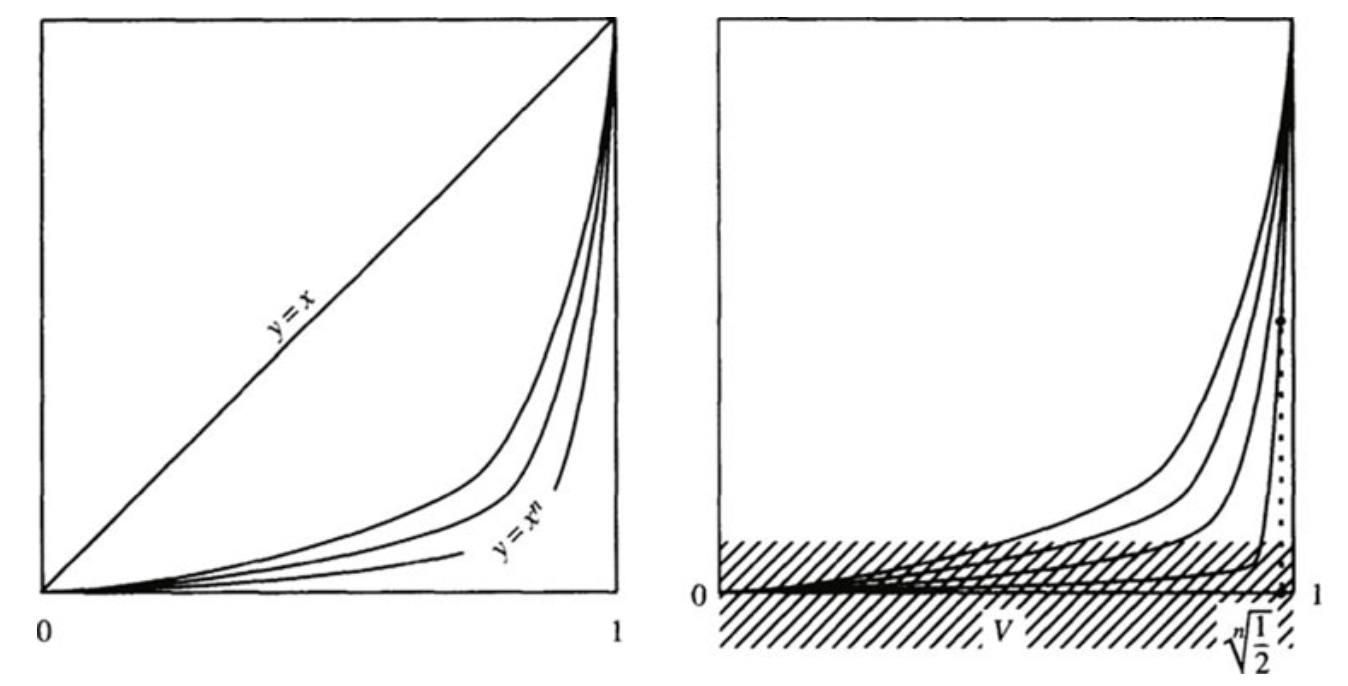
\includegraphics[scale=0.5]{ra_fig88}
\caption{Figure 88 from Section 4.1, p. 213 of \citet{pugh2015real}}
\label{ra.fig.88}
\end{center}
\end{figure}


\end{example}

\begin{proposition} In Example \ref{ra.ex.4.1.212}, if we restrict \(f_n\) and \(f\) to the open interval from 0 to 1 (so that \(f\) is simply the 0 function on this interval) \(f_n\) does not converge uniformly to \(f\) on this interval.

\end{proposition}

\begin{proof}

Suppose \(f_n\) converges uniformly to 0 (the pointwise limit). Take \(\epsilon = 1/2\). Can choose \(N \geq 1\) such that  \(|x^n - 0 | < 1/2\) for all \(n \geq N\), and for all \(x \in (0,1)\). Let \(x = (3/4)^{1/N}\). (\(N\)th roots exist by IVT.) Then \(|x^N - 0| = 3/4 \) which is not less than 1/2. 

\end{proof}

\begin{exercise}\label{ra.425b.bounded}

Let \(X\) be a set, \((Y, d)\) be a metric space. Let \(x_0 \in X\) be fixed. Let \(f: X \to Y\) be a function. Then the following are equivalent:

\begin{enumerate}

\item There exists \(m \in \mathbb{R}\) such that \(d(f(x_0), f(x)) \leq m\) for all \(x \in X\). 

\item There exists \(x_1 \in X\) and \(m \in \mathbb{R}\) such that \(d(f(x_1), f(x_2)) \leq m\) for all \(x_2 \in X\).

\item There exists \(m \in \mathbb{R}\) such that \(d(f(x_1), f(x_2)) \leq m\) for all \(x_1, x_2 \in  X\). 

\end{enumerate}

\end{exercise}

\begin{definition}

If \(f:X \to (Y, d)\) satisfies the statements in Exercise \ref{ra.425b.bounded}, then \(f\) is called \textbf{bounded.}

\end{definition}

\begin{definition}[\textbf{\(C_b(X,Y)\); defined Section 4.1 of \citet{pugh2015real}, p. 224 of pdf}]

Let \(X\) be a set and \((Y,d)\) be a metric space. Define \(C_b(X,Y)\) as the set of bounded functions from \(X\) to \(Y\). 



\end{definition}

We would like to define a metric on \(C_b(X,Y)\) related to uniform convergence. Key point: metric \(d: X \times X \to \mathbb{R} \), \textbf{not} \(\mathbb{R} \cup \infty\). That is, any two points in the metric space must be finite distances away from each other (which is why we need boundedness). We will set this up with this lemma.

\begin{lemma}

If \(f, g \in C_b(X,Y)\), then 

\[
\underbrace{\sup_{x \in X} d(f(x), g(x))}_{\text{will use for distance}} < \infty.
\]


\end{lemma}

\begin{proof}

Let \(x_0 \in X\). Choose \(M, N\) such that \(d(f(x), f(x_0) ) \leq M\) for all \(x \in X\) and \(d(g(x), g(x_0)) \leq N\) for all \(x\) (these exist since \(C_b(X,Y)\) consists of bounded functions). Then for \(x \in X\), we have

\[
d(f(x), g(x)) \leq d(f(x), f(x_0)) + d(f(x_0), g(x_0)) + d(g(x_0), g(x)) \leq \underbrace{M + d(f(x_0), g(x_0)) + N}_{\text{finite quantity independent of } x}
\]

Since this upper bound is finite, the result follows.

\end{proof}

\begin{definition}[\textbf{Sup metric; defined Section 4.1 of \citet{pugh2015real}, p. 224 of pdf}]

For \(f, g \in C_b(X, Y)\), let \(d_\infty(f, g) := \sup_{x \in X} d(f(x), g(x))\). 

\end{definition}

\begin{exercise}

The metric space axioms hold for \(d_\infty(f, g)\).

\end{exercise}

\begin{theorem}[\textbf{Theorem 4.2 in \citet{pugh2015real}}]

\(X\) set, \((Y,d)\) metric space. If \(f_n \in C_b(X, Y)\) for \(n \geq 1\) and \(f \in C_b(X, Y)\), then \(f_n\) converges uniformly to \(f\) if and only if \(f_n \xrightarrow{d_\infty} f)\). 

\end{theorem}

\begin{proof}

\(f_n\) converges uniformly to \(f\) if and only if for every \(\epsilon > 0\) there exists \(N \geq 1\) such that for all \(n \geq N\), \(d(f_n(x), f(x)) < \epsilon/2\) for all \(x \in X\). This is true if and only if for every \(\epsilon > 0\) there exists \(N \geq 1\) such that for all \(n \geq N\), 

\[
\sup_{x \in X} d(f_n(x), f(x)) = d_\infty(f_n, f) \leq \epsilon/2 < \epsilon,
\]

so \(f_n \xrightarrow{d_\infty} f\).

\end{proof}

Does this adequately characterize uniform convergence of bounded functions? yes.

\begin{proposition}[Uniform convergence preserves boundedness]

If \(f_n: X \to Y\) is bounded for all \(n\) and \(f_n\) converges uniformly to \(f\), then \(f\) is bounded.

\end{proposition}

\begin{proof}

Let \(x_0 \in X\). By uniform convergence, can choose \(N \geq 1\) such that for all \(n \geq N\) and all \(x \in X\), we have \(d(f_n(x), f(x)) < 1\). We know \(f_N\) is bounded; this implies there exists \(M\) such that \(d(f_N(x), f_N(x_0)) \leq M\) for all \(x \in X\). Note that

\[
d(f(x), f(x_0)) \leq d(f(x), f_N(x)) + d(f_N(x), f_N(x_0)) + d(f_N(x_0), f(x_0)) \leq 1 + M + 1 = M + 2
\]

which does not depend on \(x\). This implies \(f\) is bounded.

\end{proof}

\begin{corollary}[\textbf{similar to Theorem 4.2 in \citet{pugh2015real}}]

If \(f_n \in C_b(X, Y)\) for \(n \geq 1\), then \((f_n)\) converges uniformly if and only if \((f_n)\) converges in \(C_b(X, Y)\). (functional analysis perspective of uniform convergence.)

\end{corollary}

Now study metric space properties of \(C_b(X, Y)\). For now: if \(Y\) is complete then \(C_b(X,Y)\) is complete: every Cauchy sequence in \(C_b(X,Y)\) converges. But this result isn't unique to bounded functions.

\begin{definition}

\(X\) set, \((Y,d)\) metric space. A sequence of functions \(f_n: X \to Y\) is \textbf{uniformly Cauchy} if for every \(\epsilon >0\) there exists \(N \geq 1\) such that for \(n, m \geq N\) we have \(d(f_n(x), f_m(x)) < \epsilon\) for all \(x \in X\).

\end{definition}

If all \(f_n\) are bounded, then a sequence is uniformly Cauchy if and only if the sequence is Cauchy in \(C_b(X, Y)\).

\begin{theorem}\label{ra.thm.tricky}

\(X\) set, \((Y,d)\) metric space. If \((Y, d)\) is complete, then any uniformly Cauchy sequence of functions \(f_n: X \to Y\) is uniformly convergent.

\end{theorem}

\begin{proof}

Let \(f_n: X \to Y\) for \(n \geq 1\) be a uniformly Cauchy sequence. First we will show \(f_n\) converges pointwise. Then we will show the convergence is uniform. 

Given \(x \in X\), the sequence \((f_n(x))_{n=1}^\infty\) is a Cauchy sequence in \(Y\) since

\[
d(f_n(x_0), f_m(x_0)) \leq \sup_{x \in X} \left\{d(f_n(x), f_m(x)) \right\} = d_\infty(f_n, f_m).
\]

 Since \(Y\) is complete, \((f_n(x))_{n=1}^\infty\) converges to some point of \(Y\). Call this point \(f(x)\). (Limits are unique implies \(f\) is well-defined.) So by construction, \(f_n \to f\) pointwise. Next we will show that it converges uniformly.

%Given \(\epsilon\), we want to choose \(N\) and show that inequality holds for all \(x \in X\), for all \(n \geq N\). 

Let \(\epsilon > 0\). By the uniform Cauchy condition, there exists \(N \in \mathbb{N}\) such that if \(n, m \geq N\), then  \(d_\infty(f_n, f_m)) < \epsilon/2\). 

We will now show that for all \(n \geq N\) and all \(x \in X\), we have \(d(f_n(x), f(x)) < \epsilon\). Given \(x \in X\), the sequence \((f_n(x))_{n=1}^\infty\) converges to \(f(x)\) in \(Y\). Thus, we can choose \( M^*(x)\) such that for \(m \geq M^*(x)\), we have \(d(f_m(x), f(x)) < \epsilon/2\). Define \(M(x) := \max\{M^*(x), N)\). Now, for \(n \geq N\) we have 

\[
d(f_n(x), f(x)) \leq d(f_n, f_{M(x)}) + d(f_{M(x)}(x), f(x)) < \underbrace{\epsilon/2}_{\text{uniform Cauchy condition}} + \epsilon /2 = \epsilon.
\]



\end{proof}

\begin{corollary}[\textbf{Theorem 4.3 in \citet{pugh2015real}}]\label{ra.pugh.thm.4.3}

If \((Y, d)\) is complete then \((C_b(X, Y), d_\infty)\) is complete.

\end{corollary}

\begin{proof}

Cauchy sequence \((f_n)\) in \(C_b(X,Y)\) is uniformly Cauchy by Theorem \ref{ra.thm.tricky}. So it is uniformly convergent. Since uniform convergence preserves boundedness, limit \(f\) must be in \(C_b(X,Y)\), so \(f_n  \) converges to a limit in the metric space \(C_b\). 

\end{proof}

Note: if \((f_n)\) is uniformly convergent then it's uniformly Cauchy.

%Next time: look at \ and replace \((Y,d)\) with normed vector space \((V, \lVert \cdot \rVert)\).


\begin{definition}

Assume both \((X, d)\) and \((Y, d')\) are metric spaces. \((C^0(X,Y) \subset C_b(X,Y)\) is the set of bounded continuous functions \(X \to Y\). We can restrict \(d_\infty\) to \(C_0(X,Y)\) and get a metric subspace.

\end{definition}

\begin{corollary}[\textbf{Corollary to Theorem \ref{ra.thm.41.pugh}; Corollary 4.4 in \citet{pugh2015real}}]\label{ra.thm.41.pugh.cor2}

\(C^0(X,Y)\) is a closed subset of \(C_b(X,Y)\).

\end{corollary}

\begin{proof}

If we have a sequence in \(C^0(X,Y)\) that converges in \(d_\infty\) to some \(f \in C_b(X,Y)\), we want to show that \(f \in C^0\). But \(f_n\) converges uniformly to \(f\), so \(f\) is bounded and continuous by Theorem \ref{ra.thm.41.pugh}, so \(f \in C^0(X, y)\). 


\end{proof}

\begin{corollary}[\textbf{Corollary to Theorem \ref{ra.thm.tricky}}]\label{ra.thm.complete.c0}

If \((Y, d')\) is complete then \(C^0(X,Y)\) is complete. 

\end{corollary}

\begin{proof}

A closed subset of a complete metric space is complete as a metric subspace. (Closure comes from Corollary \ref{ra.thm.41.pugh.cor2}.)

\end{proof}

\begin{theorem}[\textbf{Dini's Theorem (Math 425B homework 1)}]\label{ra.dini.thm}
Let $X$ be a compact metric space and let $f_n: X \to \mathbb{R}$ be a sequence of continuous functions. Assume that the functions $f_n$ converge pointwise to $f: X \to \mathbb{R}$, that $f$ is continuous, and that for all $x \in X$, the sequence $(f_n(x))_{n=1}^{\infty}$ is a decreasing sequence of real numbers. Then $f_n$ converges uniformly to $f$.
\end{theorem}

\begin{proof}

Consider an arbitrary \(\epsilon > 0\). For each \(n \in \mathbb{N}\), consider the set \(U_n := \{x : f_n(x) - f(x) < \epsilon\} \subseteq X\). First we will show that \(U_n\) is open. If \(U_n\) is empty, then it is (trivially) open. Suppose \(U_n\) is not empty and consider a point \(u \in U_n\). \(f_n(u) - f(u) = \epsilon_u \in[0, \epsilon)\); let \(\epsilon' := \epsilon - \epsilon_u\), so \(\epsilon' \in (0, \epsilon]\). Since \(f\) and \(f_n\) are continuous, \(f_n - f\) is continuous, so there exists a \(\delta > 0\) such that \(t, u \in X\) and \(d(t, u) < \delta \implies |f_n(t) - f(t) - (f_n(u) - f(u))| < \epsilon'\). But

\begin{multline*}
\left|f_n(t) - f(t) - (f_n(u) - f(u)) \right|  < \epsilon' \iff  f_n(u) - f(u)  - \epsilon' < f_n(t) - f(t) < f_n(u) - f(u)  + \epsilon'
\\ \implies f_n(t) - f(t) < \epsilon_u + \epsilon' = \epsilon;
% \leq |f_n(t) - f(t)| +  |f_n(u) - f(u)| =  f_n(t) - f(t) +  f_n(u) - f(u) < f_n(t) - f(t) + \epsilon
% = |f_n(t) -  f_n(u) + f(u) - f(t) ]| 
%\\ \implies |f_n(t) - f(t)| < \epsilon;
\end{multline*}

 that is, all such \(t\) are in \(U_n\). The open set \(\{t: t \in X, d(t, u) < \delta \}\) is therefore a subset of \(U_n\). \(U_n\) either consists of one set like this or the union of more than one such set; either way, \(U_n\) is open.

Next we will show that the \(U_n\) cover \(X\); that is, \(X \subseteq \bigcup_{n=1}^\infty U_n\). Since \(f_n\) converges pointwise to \(f\), we know that for any \(x \in X\) there exists a finite \(N_x \in \mathbb{N}\) such that for \( n \geq N_x\) we have \(| f_n(x) - f(x) | = f_n(x) - f(x)  < \epsilon\). Let \(N^* := \max_x \{N_x\}\) (this quantity is well-defined since \(X\) is compact). Then for all \(n \geq N^*\) we have that for all \(x \in X\), \(f_n(x) - f(x)  < \epsilon\), so \(X \subseteq \bigcup_{n=N^*}^\infty U_n \subseteq \bigcup_{n=1}^\infty U_n\).

Next, consider \(n < n'\) for \(n, n' \in \mathbb{N}\). We will show that since \(U_n = \{x : f_n(x) - f(x) < \epsilon\} \) and \(U_{n'} = \{x : f_{n'}(x) - f(x) < \epsilon\} \), 

\begin{equation}\label{realan.425b.hw1.1a}
U_n \subseteq U_{n'} \qquad \forall n, n' \in \mathbb{N}, n < n'
\end{equation}

by the following argument. Consider any \(u \in U_n\). \(u\) satisfies \(f_n(u) - f(u) < \epsilon\). Since \(f_{n'}(u) \leq f_n(u)\), \(u\) also satisfies \(f_{n'}(u) - f(u) < \epsilon\), so \(u \in U_{n'}\)\footnote{Note that \(U_n\) is not necessarily a proper subset of \(U_{n'}\). For example, consider \(f(x) := 0\) and the sequence of functions defined by \( f_n(x) := 1/n\); note that these functions satisfy the assumptions of this theorem. Let \(\tilde{n} := \min \left\{n  \in \mathbb{N} : 1/n < \epsilon \right\}\). Then

\[
U_n = \begin{cases}
X, & n \geq \tilde{n}, \\
\emptyset, & n < \tilde{n},
\end{cases}
\]

so for any \(n, n' \in \{1, \ldots, \tilde{n} - 1\}\) or \(n, n' \in \{\tilde{n}, \tilde{n}+1, \ldots\}\), we have that \(U_n = U_n'\).}.

\(X\) is compact, so there exists a reduction of \(\bigcup_{n=1}^\infty U_n\) to a finite subcover of \(X\); that is, there exists a finite set \(\mathcal{S} \subset \mathbb{N}\) such that \(\bigcup_\mathcal{S} U_n = X\). Let \(s^* := \max\{\mathcal{S}\}\) (of course \(s^* < \infty\) since \(\mathcal{S}\) is finite). By (\ref{realan.425b.hw1.1a}), we have that for any \(s \in \mathcal{S}\), \(U_s \subseteq U_{s^*}\). Therefore \(X = \bigcup_\mathcal{S} U_n = U_{s^*}\), so for all \(n \geq s^*\) and all \(x \in X\), \(| (f_n(x) - f(x) | = f_n(x) - f(x)  < \epsilon\).

%Consider an arbitrary \(p \in U_n\) and \(\epsilon \in ( 0, f_1(p) - f(p))\) (note that \(\max_n \{f_n(p) - f(p)\}  =f_1(p) - f(p)\)). 
%
%By the definition from Section 2.3 of \citet{pugh2015real}, \(U_n\) is open if there exists an \(r > 0\) such that \(d(p, q) < r \implies q \in U_n\). Let \(U_n^* := \{x : f_n(x) - f(x) = \epsilon\} \subseteq X\). Select an arbitrary \(x^* \in U_n^*\), let \(r := \frac{1}{2}d(x^*, p)\).



\end{proof}






\begin{proposition}[\textbf{Uniform continuity is preserved under uniform convergence (Math 425b Homework 2)}]

%Let \(X\) and \(Y\) be metric spaces. If \(f_n: X \to Y\) is uniformly continuous for each \(n \in \mathbb{N}\) and if \(f_n\) converges uniformly to \(f\) as \(n \to \infty\), then \(f\) is uniformly continuous.

Let \((X,d)\) and \((Y, d')\) be metric spaces. Let \(f_n: X \to Y\) be uniformly continuous for all \(n \geq 1\). Suppose \(f_n\) converges uniformly to \(f\) for some \(f:X \to Y\). Then \(f\) is uniformly continuous. (This implies that if all \(f_n\) are uniformly continuous and \(f_n\) converges uniformly to \(f\) then \(f\) is uniformly continuous.)

\end{proposition}

\begin{proof}

Let \(\epsilon > 0\). Choose \(N \geq 1\) such that we have 

\begin{equation}\label{ra.425b.cauchy.1821.unif}
d'(f_n(x), f(x)) < \epsilon/3 \qquad \text{for } n \geq N \text{ and for all } x \in X.
\end{equation} 

The function \(f_N\) is uniformly continuous, so there exists \(\delta >0 \) such that

\begin{equation}\label{ra.425b.cauchy.1821.unif.2}
d'(f_N(x), f_N(x_0)) < \epsilon/3  \qquad  \forall x, x_0 \in X \text{ with } d(x, x_0) < \delta.
\end{equation} 

This \(\delta\) works for uniform continuity of \(f\) because for any \(x , x_0 \in X\) with \(d(x, x_0) < \delta\),

\[
d'(f(x), f(x_0)) \leq d'(f(x), f_N(x)) + d' (f_N(x), f_N(x_0)) + d' (f_N(x_0), f(x_0)) < \underbrace{\frac{\epsilon}{3}}_{\text{by }(\ref{ra.425b.cauchy.1821.unif})} + \underbrace{\frac{\epsilon}{3}}_{\text{by }(\ref{ra.425b.cauchy.1821.unif.2})}  + \underbrace{\frac{\epsilon}{3}}_{\text{by }(\ref{ra.425b.cauchy.1821.unif})}  = \epsilon.
\]

\end{proof}



\begin{definition}[\(C^k(X,Y)\)]

In general (say for \(\mathbb{R} \to \mathbb{R}\)): \(C^k(\mathbb{R}, \mathbb{R}) \) is the set of \(k \) times continuously differentiable functions. (Generalization of notation that \(C^0\) means continuous.) Here, we assume bounded continuity to have a \(d_\infty\) norm. For \(k=0\), metric spaces are ok. For \(k > 1\), have derivatives, so harder to generalize to metric spaces. Sometimes \(C^\infty(\mathbb{R}, \mathbb{R})\) is called the set of \textbf{smooth} functions (infinitely differentiable).

\end{definition}

If \(X\) is a set and \(V\) is a vector space (say \(\mathbb{R}\) or \(\mathbb{C}\)), then the set of functions from \(X\) to \(V\) forms a vector space itself. 

\begin{align*}
(f+g)(x) & := f(x) + g(x) \\
(cf)(x) & := c(f(x))
\end{align*}

So if \(f_n: X \to V\), makes sense to consider \(\sum_{n=1}^N f_n\), the partial sum. But we need \(V\) to also be a metric space in order to talk about convergence, so we will use a normed vector space \((V, \lVert \cdot \rVert)\). 

%(Norms have to map into \(\mathbb{R}_+\) and satisfy conditions for a metric: 0 only if identical, pull out constant, satisfy triangle inequality).

\begin{definition}[\textbf{Normed vector space}]

\((V, \lVert \cdot \rVert)\) is a \textbf{normed vector space} if \(\lVert \cdot \rVert: V \to \mathbb{R}\) satisfies

\begin{enumerate}

\item \(\lVert v \rVert \geq 0\) for all \(v\), \(\lVert v \rVert = 0 \iff v = 0\).

\item \(\lVert cv \rVert = |c| \lVert v \rVert\) for all \(c \in \mathbb{R} \) or \(\mathbb{C}\), \(v \in V\).

\item \(\lVert v +w  \rVert \leq \lVert v \rVert + \lVert w \rVert\) for all \(v, w \in V\).

\end{enumerate}

\end{definition}

More generally: \(f(V, \langle \cdot, \cdot \rangle)\) is an inner product space, can define a norm on \(V\) by \(\lVert v \rVert = \sqrt{ \langle v, v \rangle}\). But not every norm comes from an inner product. (can deduce norm axioms from inner product axioms.)

\begin{exercise}

If \((V, \lVert \cdot \rVert)\) is a normed vector space, then \(d(v,w) := \lVert v - w \rVert\) is a metric on \(V\).

\end{exercise}

So, for a vector (inner product) space it is easy to get a norm. So we can talk about \(C_b(X, V)\), etc.

Have a vector space of all functions \(X \to V\) with no restrictions. 

\begin{exercise}

\(C_b(X, V)\) is a vector subspace of all functions \(X \to V\) since if \(f, g\) are bounded then \(f + g\) is bounded and if \(f\) is bounded, then for \(c \in \mathbb{R}\) or \(c \in \mathbb{C}\), \(cf\) is bounded, and also a zero function \(X \to V\) is bounded.

\end{exercise}

So \(C_b(X, V)\) is itself a vector space. We have the metric \(d_\infty\) on the vector space \(C_b(X, V)\). Question: is there a norm on \(C_b(X, V)\) inducing the metric \(d_\infty\)? Yes, the \textbf{sup-norm} or \(\infty\)-norm.

\begin{definition}

Let \(X\) be a set and \((V, \lVert \cdot \rVert)\) be a normed vector space. If \(f \in C_b(X, V)\) then the \textbf{sup-norm} or \textbf{\(\infty\)-norm} is defined as 

\[
\lVert f \rVert_\infty = \lVert f \rVert_{\text{sup}} := \sup_{x \in X} \lVert f(x) \rVert.
\]

\end{definition}

Note that \(\lVert f \rVert_\infty = d_\infty(f,0)\). Examples: see Figure \ref{ra_sup_norm_fig}.

\begin{exercise}

\(\lVert f \rVert_\infty \) is a norm on \(C_b(X,Y)\) and \(d_\infty(f, g) = \lVert f - g \rVert_\infty\). (That is, the metric induced by \(\lVert \cdot \rVert_\infty\) is \(d_\infty\).)

\end{exercise} 



\begin{figure}[htbp]
\begin{center}
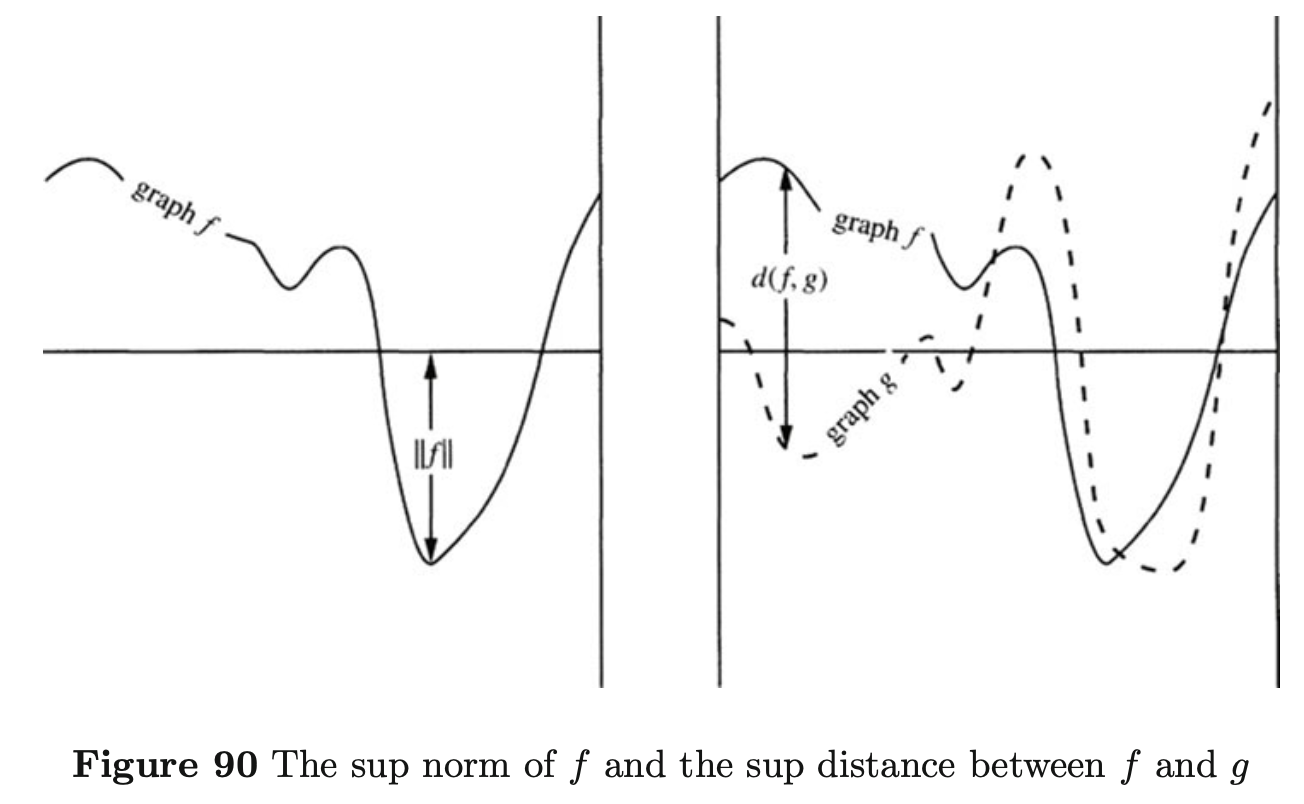
\includegraphics[scale=0.6]{ra_sup_norm}
\caption{Illustration of sup norm, Figure 90 in section 4.1 of \citet{pugh2015real}.}
\label{ra_sup_norm_fig}
\end{center}
\end{figure}

We have special terminology for complete normed vector spaces (and inner product spaces). 

\begin{definition}[\textbf{Banach space}]

A \textbf{Banach space} is a normed vector space \((V, \lVert \cdot \rVert )\) that is complete in the induced norm. (key concept in functional analysis.)

\end{definition}

\begin{definition}[\textbf{Hilbert space}]

A \textbf{Hilbert space} is an inner product space that is complete in the induced metric (a Banach space for an inner product space).

Roughly: in physics, the ``space of states" for quantum systems.

\end{definition}

Now, if \(X\) is a set and \((V, \lVert \cdot \rVert)\) is a normed vector space, we can talk about series of functions \(\sum_{n=1}^\infty f_n \) for \(f_n : X \to V\). 

\begin{definition}

Let \(X\) be a set and \((V, \lVert \cdot \rVert)\) be a normed vector space. Let \(f_n: X \to V\) be functions for \(n \in \mathbb{N}\). 

\begin{enumerate}

\item We say that the series \(\sum_{n=1}^\infty f_n\) \textbf{converges pointwise} to some \(f: X \to V\) if the sequence of partial sums 

\[
\left(  \sum_{n=1}^N f_n \right)_{N=1}^\infty 
\]

converges pointwise to \(f\).

\item We say that the series \(\sum_{n=1}^\infty f_n\) \textbf{converges uniformly} to some \(f: X \to V\) if the sequence of partial sums 

\[
\left(  \sum_{n=1}^N f_n \right)_{N=1}^\infty 
\]

converges uniformly to \(f\).

\end{enumerate}


\end{definition}

Different types of convergence for a series \(A = \sum_{n=1}^\infty v_n\) (\(v_n \in V, (V, \lVert \cdot \rVert)\) a Banach space).

Consider also a series of functions \(B = \sum_{n=1}^\infty f_n\) for \(f_n: X \to V\) with \((V, \lVert \cdot \rVert)\) a Banach space. (Absolute convergence is easiest in a Banach space, since we can use completeness.)

To show \(\sum_{n=1}^\infty v_n\)  converges in \(V\), it's enough to show the sequence of partial sums is Cauchy since \(V\) is complete. Similarly, to show that \(\sum_{n=1}^\infty f_n\) converges uniformly to \(f: X \to V\), it's enough to show the sequence of partial sums is uniformly Cauchy (again, because of completeness, which applies since we are in a Banach space).

\begin{exercise}

\begin{enumerate}[(A)]


\item Consider the series \( \sum_{n=1}^\infty v_n\) with \((V, \lVert \cdot \rVert)\) a normed vector space and \(v_n \in V\). Then 

\[
\left( \sum_{n=1}^N v_n \right)_{N=1}^\infty
\]

is Cauchy if and only if for every \(\epsilon > 0\) there exists \(N\) such that for \(N \leq m, n \) we have

\[
\left\lVert \sum_{k=m}^n v_k \right\rVert < \epsilon
\]

Note:

\[
\left\lVert  \sum_{k=1}^n v_k - \sum_{k=1}^m v_k \right\rVert = \left\lVert \sum_{k=m+1}^n v_k \right\rVert
\]

if \(n > m\). Now fix bookkeeping. 

(If seems trivial, don't worry about it, but can work out details if you want.)

\item \(X\) set, \((V, \lVert \cdot \rVert)\) a normed vector space, \(f_n: X \to V\). Then

\[
\left( \sum_{n=1}^N f_n\right)_{N=1}^\infty
\]

is uniformly Cauchy if and only if for every \(\epsilon >0\) there exists \(N\) such that for all \( N \leq m < n\) and for all \(x \in X\) we have

\[
\left\lVert \sum_{k=m}^n f_k(x) \right\rVert < \epsilon.
\]

\end{enumerate}

\end{exercise}

In the setting of \( \sum_{n=1}^\infty f_n\), have uniform vs. pointwise distinction; in both settings, have absolute vs. conditional distinction. 

\begin{definition}

Let \((V, \lVert \cdot \rVert)\) be a Banach space. A series

\[
\sum_{n=1}^\infty v_n
\]

of elements \(v_n \in V\) \textbf{converges absolutely} if the series of real numbers

\[
\sum_{n=1}^\infty \lVert v_n \rVert
\]

converges in \(\mathbb{R}\).

\end{definition}

\begin{proposition}

Let \((V, \lVert \cdot \rVert)\) be a Banach space. If 


\[
\sum_{n=1}^\infty v_n
\]

converges absolutely then it converges in \(V\).

\end{proposition}

\begin{proof}

It suffices to show that 

\[
\left( \sum_{n=1}^N v_n \right)_{N=1}^\infty
\]

is Cauchy. We know that 

\[
\left( \sum_{n=1}^N \lVert v_n \rVert \right)_{N=1}^\infty
\]

converges in \(\mathbb{R}\). Given \(\epsilon > 0\), there exists \(N\) such that for \(N \leq m < n\) we have

\[
\left| \sum_{k=m}^n \lVert v_k \rVert \right| < \epsilon.
\]

Then if \(N \leq m  < n\) we have

\[
\left\lVert \sum_{k=m}^n  v_k  \right\rVert \leq \sum_{k=m}^n \lVert v_k \rVert = \left| \sum_{k=m}^n \lVert v_k \rVert \right|  < \epsilon.
\]

So 

\[
\left( \sum_{n=1}^N v_n \right)_{N=1}^\infty
\]

is Cauchy and thus convergent.

\end{proof}

\begin{definition}

Let \(X\) be a set and let \((V, \lVert \cdot \rVert)\) be a Banach space. Let \(f_n: X \to V\). Then

\[
\sum_{n=1}^\infty f_n 
\]

\textbf{converges absolutely} if for all \(x \in X\),

\[
\sum_{n=1}^\infty f_n (x)
\]

converges absolutely. (In other words, converging absolutely means converging absolutely pointwise.)

\end{definition}



\begin{definition}[less standard naming]

Let \(X\) be a set and let \((V, \lVert \cdot \rVert)\) be a Banach space. Let \(f_n: X \to V\). Then

\[
\sum_{n=1}^\infty f_n 
\]

\textbf{converges absolutely uniformly} if 

\[
\sum_{n=1}^\infty \lVert  f_n (x) \rVert
\]

converges uniformly as a series of functions from \(X\) to \(\mathbb{R}\). (note: \( \lVert  f_n (x) \rVert\) is a function \(X \to \mathbb{R}\) whereas \(\lVert f_n \rVert_\infty = \lVert f_n \rVert_{\text{sup}}\) is a single real number, and it only exists if \(f\) is bounded.)

\end{definition}

\begin{proposition}[Absolute uniform convergence implies absolute convergence and uniform convergence]

Let \(X\) be a set and let \((V, \lVert \cdot \rVert)\) be a Banach space. Let \(f_n: X \to V\) be functions. If 

\[
\sum_{n=1}^\infty f_n
\]

converges absolutely uniformly, then it converges absolutely (pointwise) and converges uniformly.

\end{proposition}

\begin{proof}

It is clear that absolute uniform convergence implies absolute pointwise convergence. So we want to show that 

\[
\left( \sum_{n=1}^N  f_n \right)_{N= 1}^\infty
\]

converges uniformly. It is enough to show that 


\[
\left( \sum_{n=1}^N  f_n \right)_{N= 1}^\infty
\]

is uniformly Cauchy. We know that 


\[
\left( \sum_{n=1}^N \lVert f_n \rVert  \right)_{N= 1}^\infty
\]

is uniformly convergent, so it is uniformly Cauchy. Thus, given \(\epsilon > 0\) there exists \(N \in \mathbb{N}\) such that for \(N \leq m < n\) and \(x \in X\), we have

\[
\left| \sum_{k=m}^n \lVert f_k(x) \rVert \right| < \epsilon.
\]

Now if \(N \leq m < n\), then

\[
\left\lVert   \sum_{k=m}^n  f_k(x) \right\rVert \leq  \sum_{k=m}^n   \left\lVert   f_k(x) \right\rVert < \epsilon.
\]

Thus

\[
\left( \sum_{n=1}^N  f_n \right)_{N= 1}^\infty
\]

is uniformly Cauchy, and therefore uniformly convergent by the completeness of \(V\).

\end{proof}

Now look at bounded functions \(f_n: X \to V\), where \(\lVert f_n \rVert_\infty\) makes sense in \(\mathbb{R}\) (i.e. is finite). Now we can look at

\[
\sum_{n=1}^\infty \lVert f_n \rVert_\infty
\]

is a real number (series of real numbers).

\begin{theorem}[\textbf{Weierstrass M-test; Theorem 4.5 in \citet{pugh2015real}, Theorem 7.10 in \citet{rudin1976principles}, p. 148 of text/p. 157 of pdf}]\label{ra.thm.Weierstrass}


Let \(X\) be a set and let \((V, \lVert \cdot \rVert)\) be a normed vector space. Let \(f_n \in C_b(X, Y)\) be functions. If 

\[
\sum_{n=1}^\infty \lVert f_n \rVert_\infty
\]

converges as a series in \(\mathbb{R}\), then

\[
\sum_{n=1}^\infty  f_n 
\]

converges uniformly as a series of functions from \(X \to \mathbb{R}\). (Further, if \(V\) is a Banach space, it converges absolutely uniformly, so absolutely and uniformly.)



\end{theorem}

\begin{proof}

Since \(\mathbb{R}\) is complete, it suffices to show that 

\[
\left( \sum_{n=1}^N \lVert  f_n \rVert \right)_{N= 1}^\infty
\]

is uniformly Cauchy. We know that 

\[
\left( \sum_{n=1}^N \lVert  f_n \rVert_\infty \right)_{N= 1}^\infty
\]

is a Cauchy sequence in \(\mathbb{R}\). That means that given \(\epsilon > 0\), there exists \(N\) such that if \(N \leq m < n\) then

\[
\left| \sum_{k=m}^n \lVert  f_k \rVert_\infty  \right| < \epsilon.
\]

If \(N \leq m < n\) and \(x \in X\), we have

\[
\sum_{k=m}^n \lVert f_k(x) \rVert \leq \sum_{k=m}^n \sup_{x' \in X} \lVert f_k(x') \rVert = \sum_{k=m}^n \lVert f_k \rVert_\infty < \epsilon.
\]

\end{proof}

\begin{theorem}[\textbf{Weierstrass M-test, classical version, also appears in \citet{pugh2015real}}]

Let \(X\) be a set and let \((V, \lVert \cdot \rVert)\) be a Banach space. Let \(f_n: X \to V\) be bounded and suppose that for all (sufficiently large) \(n\), we have constants \(M_n \in \mathbb{R}\) such that 

\[
\lVert f_n \rVert_\infty \leq M_n, \qquad \text{and} \qquad \sum_{n=1}^\infty M_n \text{ converges.}
\]

Then \(\sum_{n=1}^\infty f_n\) converges absolutely and uniformly.

\end{theorem}

\begin{proof}

Use previous version plus comparison test for series.

\end{proof}

The Weierstrass M-test can be used to deduce uniform convergence properties for series (particularly power series). Before applying this to power series, we will study uniform convergence and integrals/derivatives. (We are still building towards showing that power series can be differentiated term-by-term inside the disc of convergence; thus they're smooth functions. Thus, power series are \(C^\infty\) in their disc of convergence.)



Integrals: let \([a,b] \in \mathbb{R}\). Let \(\mathcal{R}[a,b]\) be the set of Riemann integrable functions from \([a,b]\) to \(\mathbb{R}\) (or \(\mathbb{C}\)). Recall that (properly) Riemann integrable functions are bounded (Theorem 3.16 in \citet{pugh2015real}). So, \(\mathcal{R}[a,b] \subseteq C_b([a,b], \mathbb{R})\). 


\begin{proposition}[\textbf{Lebesgue's integrability condition}]

\(f \in C_b([a,b], \mathbb{R})\) is Riemann integrable if and only if \(\operatorname{disc}(f)\) (the set of discontinuities of \(f\)) is a \textbf{null set} (i.e., a set of measure 0.)

\end{proposition}

\begin{theorem}[\textbf{Theorem 4.6 in \citet{pugh2015real}}]\label{ra.425b.thm.4.6}

\(\mathcal{R}[a,b]\) is a closed subset of \(C_b([a,b], \mathbb{R})\), i.e.: if \(f_n \in \mathcal{R}[a,b]\) and \(f_n\) converges uniformly to some \(f \in C_b([a,b], \mathbb{R})\) (i.e., \(f_n \xrightarrow{d_\infty} f\)), then \(f \in \mathcal{R}[a,b]\). Another way to say this: the uniform limit of Riemann integrable functions is Riemann integrable. Furthermore, 

\begin{equation}\label{ra.425b.thm.4.6.eqn}
\int_a^b f(x) \ dx = \lim_{n \to \infty} \int_a^b f_n(x) \ dx;
\end{equation}

i.e.,

\[
\int_a^b \lim_{n \to \infty} f_n(x) \ dx = \lim_{n \to \infty} \int_a^b f_n(x) \ dx.
\]

\end{theorem}


\begin{proof}[Proof of Theorem \ref{ra.425b.thm.4.6}]

Use Lebesgue's integrability condition: since we know that \(f_n\) is Riemann integrable, Lebesgue's integrability condition tells us that \(\operatorname{disc}(f)\) is a null set. The countable union of null sets is a null set, so \(\bigcup_{n=1}^\infty \operatorname{disc}(f_n)\) is a null set. 

Therefore \(\operatorname{disc}(f) \subseteq \bigcup_{n=1}^\infty \operatorname{disc}(f_n)\) is a sufficient condition to show that \(f \in \mathcal{R}[a,b]\). We claim this is true. That is, we want to show that if \(x \in \operatorname{disc}(f)\), then \(x \in \operatorname{disc}(f)_n\) for some \(n\); we will prove the contrapositive. Suppose \(x \notin \operatorname{disc}(f)_n\) for any \(n\) for some \(x \in [a,b]\); that is, \(f_n\) is continuous at \(x\) for all \(n \in \mathbb{N}\). Since we assumed \(f_n\) converges uniformly to \(f\), we have that \(f\) is continuous at \(x\) from Theorem \ref{ra.thm.41.pugh}. Therefore \(x \notin \operatorname{disc}(f)\). Thus, this proves the claim, so \(f \in \mathcal{R}[a,b]\).

Next we will show that (\ref{ra.425b.thm.4.6.eqn}) holds. By uniform convergence of \((f_n)_{n=1}^\infty\) to \(f\), given \(\epsilon >0\) there exists \(N\) such that if \(n \geq N\) then \(d_\infty (f_n, f) < \epsilon/(b-a)\). Now for \(n \geq N\),

\begin{multline*}
\left|  \int_a^b f(t) \ dt - \int_a^b f_n(x) \ dx \right| = \left|  \int_a^b [f(x) - f_n(x)] \ dx \right|  \leq  \int_a^b  \left|  f(x) - f_n(x) \right| \ dx   \leq  \int_a^b d_\infty(f_n, f)  \ dx 
\\  < \frac{\epsilon}{b-a} \cdot(b-a) = \epsilon.
\end{multline*}

\end{proof}

\begin{proof}[Alternative Proof of Theorem \ref{ra.425b.thm.4.6} (425b Homework 2)]

%Lemma \ref{ra.425b.hw2.2a.lemma}


Let \(A\) be the set of tagged partitions \((P, T)\) of \([a,b]\) with the refinement ordering \(\preceq\) from Definition \ref{ra.defn.directed.set.net}. Let \(\epsilon > 0\). First we will show the nets \(R(f_n, P, T)\) converge uniformly to \(R(f, P, T)\). The nets converge uniformly if there exists \(N \in \mathbb{N}\) such that for all \(n \geq N\), for all \((P, T) \in A\) we have \( |R(f_n, P, T) - R(f, P, T)| < \epsilon\).

%That is true if there exists \(N \in \mathbb{N}\) such that for all \(n \geq N\), for all \((P, T) \in A\) we have \( |R(f_n, P, T) - R(f, P, T)| < \epsilon\).

%
%\[
%\vdots
%\]



Because the \(f_n\) converge uniformly to \(f\), we know that there exists \(N \in \mathbb{N}\) such that for all \(n \geq N\) we have that

\begin{equation}\label{ra.425b.hw2.2.d.1}
|f_n(x) - f(x)| < \frac{\epsilon}{b-a} \qquad \forall x \in [a,b].
\end{equation}


 Therefore we have that for all \((P, T)\) in \(A\) and for all \(n \geq N\),
 
\begin{multline*}
|R(f_n, P, T) - R(f, P, T)|   = \left| \sum_{i=1}^n f_n (t_i) \Delta x_i - \sum_{i=1}^n f (t_i) \Delta x_i  \right| = \left| \sum_{i=1}^n \left[ f_n (t_i) - f(t_i) \right] \Delta x_i  \right| 
\\ \leq  \sum_{i=1}^n  \left| f_n (t_i) - f(t_i) \right| \Delta x_i   \leq  \sum_{i=1}^n  \frac{\epsilon}{b-a} \Delta x_i  =   \frac{\epsilon}{b-a}  \sum_{i=1}^n \Delta x_i =  \frac{\epsilon}{b-a}  (b-a) = \epsilon.
\end{multline*}

By Proposition \ref{ra.425b.hw1.2.c}, since each function \(f_n: [a,b] \to \mathbb{R}\) is Riemann integrable, each net \((P_n,T_n) \mapsto R(f_n, P_n , T_n)\) converges to a limit \(I_n \in \mathbb{R}\). From Lemma \ref{ra.425b.hw2.2a.lemma}, we know that because this is true and because we have shown that the nets converge uniformly to \(R(f, P, T)\), the limits \((I_n)_{n=1}^\infty\) form a Cauchy sequence in \(\mathbb{R}\). Therefore by the completeness of \(\mathbb{R}\), the limits \((I_n)_{n=1}^\infty\) converge to some limit \(I \in \mathbb{R}\), which means that by Lemma \ref{ra.425b.hw2.2b.lemma} the limit of \((P, T) \mapsto R(f, P, T)\) exists and equals \(I\).

By Proposition \ref{ra.425b.hw1.2.c}, Riemann integrability of \(f\) is equivalent of convergence of the net \((P,T) \mapsto R(f, P , T)\), a net from \(A\) to \(\mathbb{R}\). Therefore, because the net \((P,T) \mapsto R(f, P, T)\) converges to \(I\), \(f\) is Riemann integrable with integral \(I\).


\end{proof}

\begin{corollary}[\textbf{Theorem 4.8 in \citet{pugh2015real}}]

If \(f_n \in \mathcal{R}[a,b]\) and the series \(\sum_{n=1}^\infty\) converges uniformly to some \(f\), then \(f \in \mathcal{R}[a,b] \) and \(\int_a^b f(x) \ dx = \sum_{n=1}^\infty \int_a^b f_n(x) \ dx\). I.e.,

\[
\int_a^b \sum_{n=1}^\infty f_n(x) dx = \sum_{n=1}^\infty \int_a^b f_n(x) \ dx.
\]

\end{corollary}

\begin{proof}

Apply Theorem \ref{ra.425b.thm.4.6} to 

\[
\left( \sum_{n=1}^N f_n \right)_{N=1}^\infty.
\]

\end{proof}

\begin{corollary}[\textbf{Corollary 4.7 in \citet{pugh2015real}}]

If \(f_n \in \mathcal{R}[a,b]\), \(f_n\) converges uniformly to \(f\), then the function \(\int_a^x f_n(t) \ dt \) converges uniformly to \(\int_a^x f(t) \ dt\). (i.e., converges uniformly in \(x \in [a,b]\).)

\end{corollary}

\begin{proof}

Similar to proof of Theorem \ref{ra.425b.thm.4.6}. Given \(\epsilon >0\), choose \(N\) such that \(d_\infty(f_n, f) < \epsilon/(b-a)\) for all \(n \geq N\). If \(n \geq N\), then 

\begin{multline*}
\left|  \int_a^x f(t) \ dt - \int_a^x f_n(t) \ dt \right| = \left|  \int_a^x [f(t) - f_n(t)] \ dt \right|  \leq  \int_a^x  \left|  f(t) - f_n(t) \right| \ dt   \leq  \int_a^x d_\infty(f_n, f)  \ dt 
\\  < \frac{\epsilon}{b-a} \cdot(b-a) = \epsilon
\end{multline*}

(since \(\int_a^x 1 \ dx \leq \int_a^b 1 \ dx = b-a\)).

\end{proof}











Question: must the uniform limit of differentiable functions be differentiable? No.

\begin{example}

Let \(f_n: [-1,1] \to \mathbb{R}\) be defined by \(f_n(x) := \sqrt{x^2 + 1/n}\). Let \(f(x) := \sqrt{x^2} = |x|\). \(f(\cdot)\)  is not differentiable at 0, but each \(f_n(x)\) is. (We will show below that \(f_n\) converges uniformly to \(f\).) So, differentiability (at one point) is lost in the limit. 

\end{example}

\begin{proposition}

\(f_n\) converges uniformly to \(f\).

\end{proposition}

\begin{proof}

We will apply Dini's Theorem (Theorem \ref{ra.dini.thm}). Note that \([-1,1]\) is a compact metric space. \(f_n(x) = \sqrt{x^2 + 1/n}\) is a sequence of continuous functions, and for all \(x \in [-1,1]\), the sequence $( \sqrt{x^2 + 1/n})_{n=1}^{\infty}$ is a decreasing sequence of real numbers since \(1/n\) is decreasing in \(n\) and \(\sqrt{\cdot}\) is a monotonic transformation in \(\mathbb{R}_+\). We also have that \(f(x) = |x|\) is continuous. 

It only remains to be shown that  the functions $f_n$ converge pointwise to \(f\). Let \(\epsilon > 0\) and let \(\tilde{x} \in [-1,1]\). We want to find \(N \in \mathbb{N}\) such that for all \(n \geq N\) it holds that \(\left|    \sqrt{\tilde{x}^2 + 1/n} - \sqrt{\tilde{x}^2}  \right| =    \sqrt{\tilde{x}^2 + 1/n} - \sqrt{\tilde{x}^2} < \epsilon\). For all \(n \geq 1\) we have

%since \( \sqrt{\tilde{x}^2 + 1/n} + \sqrt{\tilde{x}^2} \ > 0\)

%\begin{multline*}
% \sqrt{\tilde{x}^2 + 1/n} - \sqrt{\tilde{x}^2} < \epsilon \iff \left( \sqrt{\tilde{x}^2 + 1/n} - \sqrt{\tilde{x}^2} \right) \left( \sqrt{\tilde{x}^2 + 1/n} + \sqrt{\tilde{x}^2} \right) < \epsilon \left( \sqrt{\tilde{x}^2 + 1/n} + \sqrt{\tilde{x}^2} \right) 
% \\  \iff  \tilde{x}^2  + \frac{1}{n} - \tilde{x}^2  <\epsilon \left( \sqrt{\tilde{x}^2 + 1/n} + \sqrt{\tilde{x}^2} \right) 
%\iff   \frac{1}{n} <\epsilon \left( \sqrt{\tilde{x}^2 + 1/n} + \sqrt{\tilde{x}^2} \right) 
%\end{multline*}

\begin{multline*}
 \sqrt{\tilde{x}^2 + 1/n} - \sqrt{\tilde{x}^2} < \epsilon \iff   \tilde{x}^2 + \frac{1}{n} <  \left( \epsilon + \sqrt{\tilde{x}^2}  \right)^2 \iff  \frac{1}{n} < \epsilon^2 + 2 \epsilon \sqrt{\tilde{x}^2} + \tilde{x}^2 - \tilde{x}^2
 \\ \iff n > \frac{1}{\epsilon^2 + 2 \epsilon \sqrt{\tilde{x}^2}}.
\end{multline*}


Therefore set \(N := \left\lceil \left( \epsilon^2 + 2 \epsilon \sqrt{\tilde{x}^2} \right)^{-1}  + 1\right\rceil \) to complete the proof.

\end{proof}

In fact, the uniform limit of smooth functions can be nowhere differentiable (even though it is continuous, since it is the uniform limit of continuous functions.)

\begin{theorem}[\textbf{Theorem 4.9 from \citet{pugh2015real}}]\label{ra.pugh.thm.4.9}

The uniform limit of a sequence of differentiable functions is differentiable provided that the sequence of derivatives also converges uniformly.

\end{theorem}

\begin{theorem}[\textbf{Theorem 4.10 from \citet{pugh2015real}}]

A uniformly convergent series of differentiable functions can be differentiated term-by-term, provided that the derivative series converges uniformly. That is, 

\[
\deriv{}{x} \left(  \sum_{k=0}^\infty f_k(x) \right) =   \sum_{k=0}^\infty \deriv{}{x} \left( f_k(x) \right) 
\]

%not just sufficient to have \(f_n\) converge uniformly to \(f\), need stronger conditions: \(f_n\) are differentiable and \(f_n'\) converge uniformly to some \(g\). 

\end{theorem}

\begin{proof}

Apply Theorem \ref{ra.pugh.thm.4.9} to the sequence of partial sums.

\end{proof}

\begin{theorem}[\textbf{Math 425b Homework 3}]

Let \([a,b] \subset \mathbb{R}\) and let \(f_n: [a,b] \to \mathbb{R}\) be continuously differentiable (\(C^1\)) functions. Suppose that the derivatives \(f_n'\) converge uniformly to a function \(g: [a,b] \to \mathbb{R}\) and that for some \(x_0 \in [a,b]\) the function values \(f_n(x_0)\) converge to some limit \(L \in \mathbb{R}\) (i.e., \(f_n\) converges ``pointwise somewhere," a very weak condition). Then the functions \(f_n\) converge uniformly to a differentiable function \(f: [a,b] \to \mathbb{R}\) with \(f'=g\).

\end{theorem}

\begin{proof}



By the Fundamental Theorem of Calculus (Theorem 3.34 in \citet{pugh2015real}), we have that for all \(x \in [a,b]\), for a fixed \(x_0 \in [a,b]\)

\[
\int_{x_0}^x f_n'(t) \ dt = f_n(x) - f_n(x_0) =  f_n(x) - C_n \qquad \iff f_n(x) = C_n + \int_{x_0}^x f_n'(t) \ dt  
\]

where \(C_n := f_n(x_0)\).

Let \(\epsilon >0\). We have that \(f_n: [a,b] \to \mathbb{R}\) are \(C^1\) for all \(n\) and that the derivatives \(f_n'\) converge uniformly to \(g\); that is, there exists \(N' \in \mathbb{N}\) such that for all \( n \geq N'\) we have \(|f_n'(x) - g(x)| < \epsilon/(2|x-x_0|)\) for all \(x \in [a,b]\). We also have that for some \(x_0 \in [a,b]\), there exists \(N'' \in \mathbb{N}\) such that for all \(n \geq N''\), \(|f_n(x_0) - L| = |C_n - L|  < \epsilon/2\). Let \(N := \max\{N', N''\}\). Then for all \(n \geq N\) and for all \(x \in [a,b]\) it holds that 

\begin{multline*}
 \left| f_n(x) - \left(L + \int_{x_0}^x g(t) \ dt  \right) \right|  =  \left| C_n + \int_{x_0}^x f_n'(t) \ dt - \left(L + \int_{x_0}^x g(t) \ dt  \right) \right| 
 \\ = \left| C_n  - L  + \int_{x_0}^x \left[  f_n'(x) - g(x)\right]  \ dx \right|
\leq \left| C_n  - L  \right| + \left|  \int_{x_0}^x \left[  f_n'(x) - g(x)\right]  \ dx \right| \\ \leq  \left| C_n  - L  \right| + \int_{x_0}^x  \left|  \left[  f_n'(x) - g(x)\right] \right|   \ dx  <  \frac{\epsilon}{2} + |x_0 - x| \cdot \frac{\epsilon}{2|x_0 - x|}
= \epsilon;
\end{multline*}

that is, \(f_n(x)\) converges uniformly to \(L + \int_{x_0}^x g(t) \ dt\). Let \(f: [a,b] \to \mathbb{R}\) be defined by \(f(x) := L + \int_{x_0}^x g(t) \ dt\). It remains to show that \(f\) is differentiable and \(f' = g\). Again applying the Fundamental Theorem of Calculus, we have

\[
\deriv{}{x} f(x) = \deriv{}{x}  \left( L + \int_{x_0}^x g(t) \ dt \right) = \deriv{}{x}  \left( L \right) +  \deriv{}{x}  \left(  \int_{x_0}^x g(t) \ dt \right) = g(x).
\]

\end{proof}

\begin{definition}

Let \((X,d)\) and \((Y, d')\) be metric spaces and let \(f_n: X \to Y\) be a sequence of functions. Let \(f: X \to Y\) be another function. We say that \((f_n)_{n=1}^\infty\) \textbf{converges compactly} to \(f\) if for any compact subset \(K \subset X\), the restrictions of \(f_n\) to \(K\) converge uniformly to the restriction of \(f\) to \(K\). We say \((f_n)_{n=1}^\infty\) \textbf{converges locally uniformly} to \(f\) if for any \(x \in X\) there exists an open neighborhood \(U\) of \(x\) such that the restrictions of \(f_n\) to \(U\) converge uniformly to the restriction of \(f\) to \(U\).

\end{definition}

\begin{definition}

Let \((X,d)\) be a metric space. We say that \((X,d)\) is \textbf{locally compact} if for all \(x \in X\) there exists an open set \(U\) and a compact set \(K\) such that \(x \in U \subseteq K \subseteq X\).

\end{definition}

\begin{proposition}[\textbf{Math 425b Homework 3}]

Let \((X,d)\) be a locally compact metric space. Let \(f_n, f: X \to Y\) be functions. The functions \(f_n\) converge compactly to \(f\) if and only if they converge locally uniformly to \(f\).

\end{proposition}

\begin{proof}

Let \(K \subset X\) be an arbitrary compact subset of \(X\). We have that \((X, d)\) is locally compact; that is, for all \(x \in X\) there exist \(x \in U \subset K\) with \(U\) open.



\begin{itemize}

\item \textbf{Compact convergence implies local uniform convergence:} Let \(\epsilon' > 0\). Let \(K'\) be an arbitrary compact subset of \(X\). We will assume that \((f_n)_{n=1}^\infty\) converges compactly to \(f\); that is, the restrictions of \(f_n\) to \(K'\) converge uniformly to the restriction of \(f\) to \(K'\). That is, there exists \(N' \in \mathbb{N}\) such that for all \( n \geq N'\), \(d'(f_n(x), f(x)) < \epsilon'\) for all \(x \in K'\). By local compactness, for all \(x \in X\) there exists an open set \(U'\) with \(x \subset U' \subset K'\) with \(U'\) open. Since \(U' \subset K'\), it holds that  for all \( n \geq N'\), \(d'(f_n(x), f(x)) < \epsilon'\) for all \(x \in U'\). Therefore the restrictions of \(f_n\) to \(U'\) converge uniformly to the restriction of \(f\) to \(U'\).

\item \textbf{Local uniform convergence implies compact convergence:} Let \(\epsilon'' > 0\). We will assume that \((f_n)_{n=1}^\infty\) converges locally uniformly to \(f\); that is, for any \(x'' \in X\) there exists an open neighborhood \(U''\) of \(x''\) such that the restrictions of \(f_n\) to \(U''\) converge uniformly to the restriction of \(f\) to \(U''\).

We want to show that for any compact subset \(K''\) of \(X\) there exists an \(N'' \in \mathbb{N}\) such that for all \( n \geq N''\), \(d'(f_n(x), f(x)) < \epsilon''\) for all \(x \in K''\).

Consider an arbitrary compact subset \(K''\) of \(X\). For every \(\tilde{x}'' \in K''\), by assumption there exists an open set \(\tilde{U}''\) with \( \tilde{x}'' \in \tilde{U}'' \subset \tilde{K}'' \subset X\) such that the restrictions of \(f_n\) to each \(\tilde{U}''\) converge uniformly to the restriction of \(f\) to \(\tilde{U}''\). That is, for each set there exists \(\tilde{N}'' \in \mathbb{N}\) such that for all \(n \geq N\) and for all \(\tilde{x}'' \in \tilde{U}''\) it holds that \(d'(f(\tilde{x}''), f_n(\tilde{x}'')) < \epsilon\). Note that the union of all such \(\tilde{U}''\) (which might be an infinite number of sets) is an open cover of \(K''\). Because \(K''\) is compact, this open cover of \(K''\) reduces to a finite subcover, so there exists a finite number of these sets that cover \(K''\). Let the union of these sets (the finite subcover) be \(\mathcal{U}\). Among each of these sets, let \(N''\) be the maximum of all the \(\tilde{N}''\) (this number is well-defined since there is a finite number of the \(\tilde{N}''\)). Then for all \(x \in \mathcal{U}\) and for all \(n \geq N''\) it holds that \(d'(f_n(x), f(x)) < \epsilon\). Since \(K'' \subset \mathcal{U}\), the result follows.  

\end{itemize}

\end{proof}

\begin{definition} 

For \(f \in C^0([a,b], \mathbb{R})\), define \(\lVert f \rVert_1 := \int_a^b |f(x)| dx\). (The norm axioms hold for \(\lVert \cdot \rVert_1\).)

\end{definition}

For \([a,b] \subset \mathbb{R}\), consider the vector space \(C^0([a,b], \mathbb{R})\) (we could take functions into \(\mathbb{C}\) instead and have a complex vector space). We have a norm \(\lVert \cdot \rVert_\infty\) on \(C^0([a,b],\mathbb{R})\) making it into a Banach space. 

\begin{proposition}[\textbf{Math 425b Homework 3}]



If \(f_n, f \in C^0([a,b], \mathbb{R})\) and \(f_n\) converge to \(f\) in \(\lVert \cdot \rVert_\infty\) then \(f_n\) converges to \(f\) in \(\lVert \cdot \rVert\). However, the opposite does not hold; converging in \(\lVert \cdot \rVert_1\) does not imply convergence in \(\lVert \cdot \rVert_\infty\).

\end{proposition}

\begin{proof}

Let \(f_n, f \in C^0([a,b], \mathbb{R})\). Let \(\epsilon > 0\). Suppose \(f_n\) converges to \(f\) in \(\lVert \cdot \rVert_\infty\); that is, there exists \(N \in \mathbb{N}\) such that for all \(n \geq N\), \(\lVert f_n - f \rVert_\infty = \sup_{x \in [a,b]} \{ | f_n(x) - f(x)| \} < \epsilon/[2(b-a)]\). But then for all \(n \geq N\),

\[
\lVert f_n - f \rVert_1 = \int_a^b |f_n(x) - f(x)| \ dx \leq  \int_a^b \sup_{x \in [a,b]} \{ | f_n(x) - f(x)| \} \ dx  = \frac{\epsilon}{2(b-a)} \cdot(b-a) =  \frac{\epsilon}{2} < \epsilon.
\]

For a counterexample showing that converging in \(\lVert \cdot \rVert_1\) does not imply convergence in \(\lVert \cdot \rVert_\infty\), define \(f_n: [0,1] \to \mathbb{R}\) by \(f_n(x) = x^n\) and define \(f: [0,1] \to \mathbb{R}\) by \(f(x) = 0\). Clearly \(f_n, f \in C^0([0,1], \mathbb{R})\). Let \(\epsilon > 0\). Note that 

\[
\lVert f_n - f \rVert_1 < \epsilon \iff  \int_0^1 x^n \ dx < \epsilon \iff \left[ \frac{x^{n+1}}{n+1} \right]_0^1 < \epsilon \iff \frac{1}{n+1} < \epsilon \iff n > \frac{1}{\epsilon} - 1,
\]

so for all \(n \geq \left\lceil  1/\epsilon \right\rceil\) it holds that \(\lVert f_n - f \rVert_1 < \epsilon\). Therefore \(f_n\) converges to \(f\) in \(\lVert \cdot \rVert_1\). However, 

\[
\lVert f_n - f \rVert_\infty =  \sup_{x \in [0,1]} \{ | x^n | \} \geq | 1^n | = 1 \qquad \forall n \in \mathbb{N}, 
\]

so \(f_n\) does not converge to \(f\) in \(\lVert \cdot \rVert_\infty\).



\end{proof}





\begin{proposition}[\textbf{Math 425b Homework 3}]

\((C^0([0,1], \mathbb{R}), \lVert \cdot \rVert_1)\) is not complete (i.e. not a Banach space).

\end{proposition}

\begin{proof}

Let \(f_n: [0,1] \to \mathbb{R}\) be defined by

\[
f_n(x) = \begin{cases}
0, & 0 \leq x \leq \frac{n -1}{2n}, \\
\frac{1 - 0 }{1/2 - (n-1)/2n}\left( x - \frac{n-1}{2n} \right), & \frac{n -1}{2n} < x \leq 1/2, \\
%[2(1-x)]^n, & 1/2 < x \leq 1.
1, & 1/2 < x \leq 1,
\end{cases} = \begin{cases}
0, & 0 \leq x \leq \frac{n -1}{2n}, \\
2n  x - n + 1, & \frac{n -1}{2n} < x \leq 1/2, \\
%[2(1-x)]^n, & 1/2 < x \leq 1.
1, & 1/2 < x \leq 1,
\end{cases}
\]

for \(n \in \mathbb{N}\). First we will show that these functions are Cauchy in \(d_1\). Let \(\epsilon > 0\). For \(n, m \in \mathbb{N}\) with \(n < m\), we have 

\begin{align*}
& \int_0^1 | f_n(x) - f_m(x) | \ dx 
\\ = & \int_0^{(n-1)/2n}  | 0 - 0  | \ dx  + \int_{(n-1)/2n} ^{(m-1)/2m}   | 2n  x - n + 1 - 0  | \ dx 
\\ & + \int_{(m-1)/2m} ^{1/2}  | 2n  x - n + 1 - (2m  x - m + 1) | \ dx 
 + \int_{1/2}^1  | 1- 1  | \ dx
\\ = & \int_{(n-1)/2n} ^{(m-1)/2m}  ( 2n  x - n + 1 ) \ dx  + \int_{(m-1)/2m} ^{1/2}  | (n - m)  (2x - 1) | \ dx  
\\ = &  \left[ n  x^2 - (n-1)x \right]_{(n-1)/2n} ^{(m-1)/2m}   + (n - m)   \left[ x - x^2 \right]_{(m-1)/2m} ^{1/2}  
\\ = &  \left[ n  \left(\frac{m-1}{2m} \right) ^2 - (n-1)\left(\frac{m-1}{2m} \right) \right] - \left[ n  \left(\frac{n-1}{2n} \right) ^2 - (n-1)\left(\frac{n-1}{2n} \right) \right] 
\\ & \ + (n - m)   \left[ \frac{1}{2} - \frac{1}{4} - \left(\frac{m-1}{2m}  - \left[ \frac{m-1}{2m}  \right]^2 \right)  \right] 
\\ = &  \frac{n}{4} \left[ \left( \frac{m-1}{m} \right )^2 - \left( \frac{n-1}{n} \right )^2\right]   -  \left( \frac{n-1}{2} \right) \left( \frac{m - 1}{m} -  \frac{n-1}{n} \right)
\\ & \ + (n - m)   \left[  \frac{1}{4} - \frac{ 2m(m-1) - (m-1)^2}{4m^2}   \right] 
%\\ = & \ n  m^2 - (n-1)m - \left( n  \cdot n^2 - (n-1)n \right)     + (n - m)   \left[ \frac{1}{2} - \frac{1}{4} - \left(m - m^2 \right)   \right]
%\\ = & \ n  m^2  -nm + m  - n^3 +  n^2 - n     + \frac{1}{4}  (n - m) -  (n - m)\left(m - m^2 \right) 
%\\ = & \ 2nm^2  -2nm +  \frac{3}{4} m - \frac{3}{4} n   - m ^3  - n^3         + m^2 +  n^2 \
\end{align*}

\[
\vdots
\]

\end{proof}

\subsection{Power Series (Section 4.2 of \citet{pugh2015real})}

Note: if \(z_0 \in \mathbb{C}\), can consider power series \(\sum_{n=0}^\infty c_n(z - z_0)^n\) (where \(c_n \in \mathbb{C}\)): as a function of \(z \in \mathbb{Z}\). We can still use

\begin{equation}\label{ra.radius.convergence}
R = \frac{1}{ \underset{n\to\infty}{\lim \sup} |c_n|^{1/n}}
\end{equation}

and if \(|z - z_0| < R\) then the series converges absolutely, if \(|z - z_0| > R\) then the series diverges (and this is the unique \(R\) with these properties). We can call \(B_R(z_0)\) the open ball of radius \(R\) at \(z_0\) and the disk of convergence. 

\begin{theorem}[\textbf{Theorem 4.11 from \citet{pugh2015real}}]

Let \(\sum_{n=0}^\infty c_n (x - x_0)^n\) be a real power series. Let \(R\) be its radius of convergence, given by (\ref{ra.radius.convergence}). If we have \(r \in [0, R)\), then the series \(\sum_{n=0}^\infty c_n (x - x_0)^n\) converges uniformly on \([-r + x_0, r+ x_0]\).

\end{theorem}

\begin{proof}

Basic idea: use convergence of geometric series to study power series.

Chose \(\beta\) with \(r < \beta < R\); such a \(\beta\) exists since \(r < R\). Then \(1/R < 1/\beta \iff \underset{n \to \infty}{\lim \sup} |c_n|^{1/n} < 1/\beta\). Recall:

\[
\underset{n \to \infty}{\lim \sup} |c_n|^{1/n} = \lim_{n \to \infty} \left( \sup_{n' \geq n} |c_{n'}|^{1/n'} \right)
\]

(as \(n\) increases we have a smaller set that we are taking a supremum over, so the quantity we are taking the limit of is nonincreasing with \(n\).) So \(\underset{n \to \infty}{\lim \sup} |c_n|^{1/n} < 1/\beta\) implies there exists an \(n_0\) such that 

\[
\sup_{n' \geq n_0} |c_{n'}|^{1/n'} < \frac{1}{\beta};
\]

i.e., for \(n' \geq n_0\) we have 

\[
|c_{n'}|^{1/n'} < 1/\beta \iff |c_{n'}| < \beta^{-n'}.
\]

Without loss of generality, let \(x_0 = 0\).  For \(x \in [-r, r]\) and \(n \geq n_0\) we have

\[
| c_n x^n| < \beta^{-n} r^n = \underbrace{ \left( \frac{r}{\beta} \right)^n}_{:= M_n}
\]

(note that \(r/\beta < 1\)). By the Weierstrass M-test, if \(\sum_{n=n_0}^\infty M_n\) is finite then \(\sum_{n=n_0}^\infty c_n x^n\) converges uniformly on \([-r,r]\) (which is true if and only if \(\sum_{n=0}^\infty c_n x^n\) converges uniformly on \([-r,r]\)). But 

\[
\sum_{n=0}^\infty  \left( \frac{r}{\beta} \right)^n= \frac{1}{1 - r/\beta},
\]

which is finite, proving the theorem.

\end{proof}

\begin{corollary}

\(\sum_{n=0}^\infty c_n(x- x_0)^n\) converges compactly/locally uniformly on its interval of convergence \((-R + x_0, R + x_0)\).

\end{corollary}

\begin{proof}

Exercise. Show every compact subset \(K \subset (-R + x_0, R+ x_0)\) is contained in some \([-r + x_0, r+ x_0]\). 

\end{proof}

\begin{theorem}

Complex version: \(\sum_{n=0}^\infty c_n (z - z_0)^n\) converges compactly/locally uniformly on its open disk of convergence \(B_R(z_0)\).

\end{theorem}

\begin{proof}

Basically same; \(K \subset \overline{B_r}(z_0) \subset B_R(z_0)\) for some \(0 \leq r < R\) where \( \overline{B_r}\) is the closure of \(B_r\).

\end{proof}

Interlude: complex analysis approach to differentiating power series.

\begin{definition}

Let \(D \subseteq \mathcal{C}\) be open. A function \(f: D \to \mathcal{C}\) is \textbf{complex differentiable} or \textbf{holomorphic} if for each \(z. \in D\) the limit of

\[
\frac{\Delta f}{\Delta z} = \frac{f(z + \Delta z) - f(z)}{\Delta z}
\]

exists as \(\Delta z \to 0 \) in \(\mathbb{C}\). (The limit, if it exists, is a complex number.)

\end{definition}

\begin{theorem}\label{ra.complex.analysis.thm.diff.power.series}

if \(\Omega \subset \mathbb{C}\) is open, \(f_n: \Omega \to \mathbb{C}\) are \textbf{holomorphic} functions (complex differentiable) and \(f_n\) converge compactly/locally to some \(f: \Omega \to \mathbb{C}\), then \(f\) is holomorphic and \(f'(z) = \lim_{n \to \infty} f_n'(z) \).

\end{theorem}

Note that converging compactly/locally uniformly is weaker than uniform convergence. So somehow complex differentiability is easier to get than real differentiability. (Proven using different methods: Cauchy integral theorem, etc.)

Let's use this result. Apply this to power series. Note: \(\sum_{n=0}^N c_n(z- z_0)^n\) is a (complex) polynomial. Some basic facts about complex differentiability: it's holomorphic and 

\[
\deriv{}{z} \left( \sum_{n=0}^N c_n(z- z_0)^n\right)  
\]

can be differentiated using the usual rules for real number differentiation. Thus by the above theorem, complex power series can be (complex) differentiated term-by-term on their disk of convergence implies (not hard to prove) version. for real series, we'll give a different proof. 

\begin{theorem}[\textbf{Theorem 4.12 in \citet{pugh2015real}}]\label{ra.diff.int.power.series}

Let \(\sum_{k=0}^\infty c_k(x - x_0)^k\) be a real power series. Let \(R\) be its radius of convergence. Then \(\sum_{k=0}^\infty c_k (x - x_0)^k\) is differentiable on \((- R + x_0, R + x_0)\) with derivative \(\sum_{k=1}^\infty k c_k(x- x_0)^{k-1}\), which has the same radius of convergence.

In particular, the differentiated series 
\[
\sum_{k=1}^{\infty} kc_k (x-x_0)^{k-1}
\]
and the integrated series 
\[
\sum_{k=0}^{\infty} \frac{c_k}{k+1}(x-x_0)^{k+1}
\]
have the same radius of convergence $R$ as the original series $\sum_{k=0}^{\infty} c_k (x-x_0)^k$.


(crucial fact about power series: you can differentiate them like you'd like to.)

\end{theorem}

To prove this, we will need some lemmas.

\begin{lemma}[\textbf{Math 425b Homework 4}]\label{ra.425b.hw4.lemma.1}

%Suppose \(a_n, b_n\) are sequences of nonnegative real numbers. Then \(\sup a_n b_n \leq \sup a-n \sup b_n\) as long as the right side of the inequality is not an indeterminate form \(0 \times \infty\) or \(\infty \times 0\).

Suppose $a_n, b_n$ are sequences of real numbers with $a_n \geq 0$ and $b_n \geq 0$ for all $n$. Show that $\sup a_n b_n \leq \sup a_n \sup b_n$, as long as the right side of the inequality is not an indeterminate form $0 \times \infty$ or $\infty \times 0$.

\end{lemma}

\begin{proof}

Suppose \(\sup_n a_n \in (-\infty, \infty ), \sup_n b_n \in (-\infty, \infty)\). Let \(n' \in \mathbb{N}\). Observe that \(a_{n'} b_{n'} \leq \sup_n \{a_n\}  b_{n'} \leq  \sup_n \{a_n\}  \sup_n \{b_n\} \). Since this statement is true for all \(n\), it follows that \(\sup_n \{a_n b_n\} \leq   \sup_n \{a_n\}  \sup_n \{b_n\} \).

Clearly \(\sup_n a_n > -\infty\) and \(\sup_n b_n > -\infty\) (in fact, \(\sup_n a_n \geq 0\) and \(\sup_n b_n \geq 0\)), so the only other cases we need to consider are if one or both of the suprema equal infinity. But if this is true, then \(\sup_n \{a_n\} \sup_n \{b_n\} = \infty\) and the inequality holds trivially.


\end{proof}

\begin{lemma}[\textbf{Math 425b Homework 4}]\label{ra.425b.hw4.lemma.2}

 Suppose $a_n, b_n$ are sequences of real numbers with $a_n \geq 0$ and $b_n \geq 0$ for all $n$. Then
\[
\lim \sup a_n b_n \leq \lim \sup a_n \lim \sup b_n,
\]
as long as the right side of the inequality is not an indeterminate form $0 \times \infty$ or $\infty \times 0$ (and we can assume the limit of a product sequence is equal to the product of limits).

\end{lemma}

\begin{proof}

Recall that \(\lim \sup a_n b_n = \lim_{N \to \infty} \sup_{n \geq N} \{ a_n b_n \}\). For a fixed \(N \in \mathbb{N}\), consider the sequences \(\left(\tilde{a}_n^{(N)}  \right)_{n=1}^\infty\) and \(\left(\tilde{b}_n^{(N)} \right)_{n=1}^\infty\)  defined by


\[
\tilde{a}_n^{(N)}  = \begin{cases}
0, & n < N ,\\
a_n  & n \geq N,
\end{cases} \qquad \text{and} \qquad
 \tilde{b}_n^{(N)} = \begin{cases}
0, & n < N ,\\
 b_n, & n \geq N.
\end{cases}
\]

Note that \( \sup \tilde{a}_n^{(N)} = \sup_{n \geq N} a_n  \), etc. Since these are sequences of nonnegative real numbers for all \(N \in \mathbb{N}\), we know from Lemma \ref{ra.425b.hw4.lemma.1} that $\sup \tilde{a}_n^{(N)}  \tilde{b}_n^{(N)} \leq \sup \tilde{a}_n^{(N)} \sup  \tilde{b}_n^{(N)}$ for all \(n \in \mathbb{N}\) and \(N \in \mathbb{N}\) as long as the right side of the inequality is not an indeterminate form $0 \times \infty$ or $\infty \times 0$. Then

\begin{align*}
\sup \tilde{a}_n^{(N)}  \tilde{b}_n^{(N)} & \leq \sup \tilde{a}_n^{(N)} \sup  \tilde{b}_n^{(N)}
\\ \iff \lim_{N \to \infty} \left( \sup \tilde{a}_n^{(N)}  \tilde{b}_n^{(N)} \right)  & \leq  \lim_{N \to \infty} \left(  \sup \tilde{a}_n^{(N)} \sup  \tilde{b}_n^{(N)} \right)
\\ \iff \lim_{N \to \infty} \left( \sup \tilde{a}_n^{(N)}  \tilde{b}_n^{(N)} \right)  & \leq  \lim_{N \to \infty} \left(  \sup \tilde{a}_n^{(N)} \right)  \lim_{N \to \infty} \left( \sup  \tilde{b}_n^{(N)} \right)
\\ \iff \lim_{N \to \infty} \left( \sup_{n \geq N} a_n  \tilde{b}_n^{(N)} \right)  & \leq  \lim_{N \to \infty} \left(  \sup_{n \geq N} a_n \right)  \lim_{N \to \infty} \left( \sup_{n \geq N}  b_n \right)
\\ \iff \lim \sup a_n b_n & \leq \lim \sup a_n \lim \sup b_n,
\end{align*}

where we used the assumption that the limit of a product sequence is equal to the product of limits.

%\[
%\tilde{a}_n^{(N)} \tilde{b}_n^{(N)} = \begin{cases}
%0, & n < N \\
%a_n b_n, & n \geq N
%\end{cases}.
%\]

% \(\left(\tilde{a}_n^{(N)} \tilde{b}_n^{(N)} \right)_{n=1}^\infty\) 

%Consider the sequence \(\left(\sup_{n \geq N} \{ a_n b_n \} \right)_{N=1}^\infty\). 

\end{proof}

\begin{lemma}[\textbf{Math 425b Homework 4}]\label{ra.425b.hw4.lemma.3}

Suppose $a_n, b_n$ are sequences of real numbers with $a_n \geq 0$ and $b_n \geq 0$ for all $n$. Assume that $\lim_{n \to \infty} a_n = A$ with $0 < A < \infty$, and write $B = \lim \sup b_n \in [0,\infty]$. Show that
\[
\lim \sup a_n b_n = AB.
\]

\end{lemma}

\begin{proof}

If \(B = \infty\), it holds trivially that \(\lim \sup a_n b_n \leq AB\). Suppose \(B \in [0, \infty)\). Since \(\lim_{n \to \infty} a_n = A \in \mathbb{R}_+\) and \(\lim \sup b_n = B \in \mathbb{R}_+\), it holds that \(\lim \sup a_n = \lim a_n = A\) and likewise for \(b_n\). Then by Lemma \ref{ra.425b.hw4.lemma.2}

\[
 \lim \sup a_n b_n  \leq \lim \sup a_n \lim \sup b_n = \lim a_n \lim b_n = AB.
\]

Now we will show the reverse inequality. First, suppose \(B \in [0,\infty)\). Let \(\epsilon > 0\). Because \(\lim a_n = A\), there exists \(N_a\) such that for all \(n \geq N_a\) we have \(|a_n - A| < \epsilon \implies a_n > A - \epsilon\). Since \(a_n, b_n \geq 0\) it follows that for all \(N \geq N_a\)

\[
 \sup_{n \geq N} a_n b_n \geq  \sup_{n \geq N} (A - \epsilon) b_n =  (A - \epsilon) \sup_{n \geq N}  b_n = (A - \epsilon) B.
 \]
 
 Therefore it follows from the \(\epsilon\)-principle (Theorem 1.8 in \citet{pugh2015real}) that \( \sup_{n \geq N} a_n b_n  \geq AB\) for all sufficiently large \(N\), which in turn implies \( \lim \sup a_n b_n  \geq AB\).
 
 Now suppose \(B = \infty\). We have that there exists \(N_a'\) such that for all \(n \geq N_a'\), \(|A - a_n| < A/2 \implies a_n > A - A/2 = A/2\). Let \(M \in \mathbb{R}_+\). Similarly, here exists \(N_b'\) such that for all \(n \geq N_b'\), \(b_n \geq 2M/A\). Let \(N' := \max\{N_a', N_b'\}\), then for all \(n \geq N'\) it holds that \(a_n b_n > (A/2)(2M/A) = M\). Since \(M\) is arbitrary, it follows that in this case \( \lim \sup a_n b_n  \geq M\) for any \(M \in \mathbb{R}_+\); that is, \( \lim \sup a_n b_n  = \infty\).

%\[
%\lim \sup a_n b_n = \lim_{N \to \infty} \sup_{n \geq N} a_n b_n 
%\]
%
%\[
%\vdots
%\]
%
%From Theorem 1.5 in \citet{pugh2015real} we know that since \((a_n)\) and \((b_n)\) converge to finite limits, \((a_n)\) and \((b_n)\) are bounded; that is, there exists \(M \in \mathbb{R}\) such that \(a_n \leq M, b_n \leq M\) for all \(n \in \mathbb{N}\). Therefore \(a_n b_n \leq M^2 < \infty \) for all \(n \in \mathbb{N}\); that is, \(a_n b_n\) is bounded.

\end{proof}

Now we can prove the main result.

\begin{proof}[Proof of Theorem \ref{ra.diff.int.power.series} (from Homework 4, Math 425b)]

We will rely on the identies 

\begin{equation}\label{ra.425b.hw4.eqn.4}
\lim_{k \to \infty} k^{1/k} = 1, \qquad \lim_{k \to \infty} \left(\frac{1}{k+1} \right)^{1/k} = 1 
\end{equation}

and

\begin{equation}\label{ra.425b.hw4.eqn.5}
\lim \sup \sqrt[k]{k |c_k|} = \lim \sup \sqrt[k]{|c_k|} = \lim \sup \sqrt[k]{\frac{|c_k|}{k+1}},
\end{equation}

which we will prove later. Assuming these hold, note that by Theorem 3.44 in \citet{pugh2015real}, the radius of convergence of the power series $\sum_{k=0}^{\infty} c_k (x-x_0)^k$ is

\[
R = \frac{1}{\underset{k \to \infty}{\lim \sup} \sqrt[k]{|c_k|}}.
\]

We will show that \(\sum_{k=1}^{\infty} kc_k (x-x_0)^{k-1} = \sum_{k'=0}^{\infty} (k' + 1)c_{k' + 1} (x-x_0)^{k'}\) and \(\sum_{k=1}^{\infty} kc_k (x-x_0)^{k}\) have the same radii of convergence using the Root Test (Theorem 3.42 in \citet{pugh2015real}). Let the radius of convergence of the first series be \(R_1'\) and the radius of convergence of the second series be \(R_1\). Then in the first case, by Lemma \ref{ra.425b.hw4.lemma.3}

\begin{multline*}
\underset{k' \to \infty}{\lim \sup}  \sqrt[k']{ |(k' + 1)c_{k' + 1} |} = \underset{k' \to \infty}{\lim \sup} (k' + 1)^{1/k'} |c_{k' + 1} |^{1/k'} = \underset{k' \to \infty}{\lim \sup} (k' + 1)^{1/k'}  \cdot \underset{k' \to \infty}{\lim \sup}  |c_{k' + 1} |^{1/k'}
\\ = \lim_{k' \to \infty} \sup_{n' \geq k'} \left\{ (n' + 1)^{1/n'}  \right\} \cdot \lim_{k' \to \infty} \sup_{n' \geq k'} \left\{  |c_{n' + 1} |^{1/n'} \right\} = \lim_{k' \to \infty} \sup_{n' \geq k'} \left\{ {n'} ^{1/n'}  \right\} \cdot \lim_{k' \to \infty} \sup_{n' \geq k'} \left\{  |c_{n' } |^{1/n'} \right\}
\end{multline*}

%are equal because the radius of convergence of the first is




\[
\implies R_1' = \frac{1}{\underset{k' \to \infty}{\lim \sup} \sqrt[k']{| (k' + 1)c_{k' + 1}|}} = \frac{1}{ \lim_{k' \to \infty} \sup_{n' \geq k'} \left\{ \sqrt[n']{n'  | c_{n' }|} \right\} }
%\\ = \frac{1}{ \lim_{k' \to \infty} \sup_{n'' \geq k' + 1} \left\{ \sqrt[n'' - 1]{n'' | c_{n''}|} \right\} }
\]



and the radius convergence of the second is

\[
R_1 =  \frac{1}{\underset{k \to \infty}{\lim \sup} \sqrt[k]{|k c_k|}} = \frac{1}{ \lim_{k \to \infty} \sup_{n \geq k} \left\{ \sqrt[n]{n | c_{n}|} \right\} } = R_1'.
\]



Similarly, let the radius of convergence of \(\sum_{k=0}^\infty \frac{c_k}{k+1}(x - x_0)^{k+1} = \sum_{k'=1}^\infty \frac{c_{k'-1}}{k'}(x - x_0)^{k'}\) be given by \(R_2'\) and the radius of convergence of \(\sum_{k=0}^\infty \frac{c_k}{k+1} (x - x_0)^k\) be given by \(R_2\). Then in the first case, by Lemma \ref{ra.425b.hw4.lemma.3}


\begin{multline*}
\underset{k' \to \infty}{\lim \sup}  \sqrt[k']{ \left|\frac{c_{k'-1}}{k'} \right|} = \underset{k' \to \infty}{\lim \sup} \left\{ {k'}^{-1/k'} |c_{k' - 1} |^{1/k'}  \right\} = \underset{k' \to \infty}{\lim \sup} \left\{ {k'}^{-1/k'} \right\}  \underset{k' \to \infty}{\lim \sup} \left\{  |c_{k' - 1} |^{1/k'}  \right\}
\\ = \lim_{k' \to \infty} \sup_{n' \geq k'} \left\{ {n'}^{-1/n'}  \right\} \cdot \lim_{k' \to \infty} \sup_{n' \geq k'} \left\{  |c_{n' - 1} |^{1/n'} \right\} = \lim_{k' \to \infty} \sup_{n' \geq k'} \left\{ {(n' + 1)} ^{-1/n'}  \right\} \cdot \lim_{k' \to \infty} \sup_{n' \geq k'} \left\{  |c_{n' } |^{1/n'} \right\}
\end{multline*}




\[
\implies R_2' = \frac{1}{\underset{k' \to \infty}{\lim \sup} \sqrt[k']{| \frac{c_{k'-1}}{k' + 1}|}} = \frac{1}{ \lim_{k' \to \infty} \sup_{n' \geq k'} \left\{ \sqrt[n']{(n'+1)^{-1} | c_{n'}|} \right\} }
\]



and the radius convergence of the second is

\[
R_2 =  \frac{1}{\underset{k \to \infty}{\lim \sup} \sqrt[k]{\left| \frac{c_k}{k + 1} \right|}} = \frac{1}{ \lim_{k \to \infty} \sup_{n \geq k} \left\{ \sqrt[n]{(n+1)^{-1} | c_{n}|} \right\} } = R_2'.
\]





Next, observe that the radius of convergence of \(\sum_{k=1}^{\infty} kc_k (x-x_0)^{k}\) (and therefore the radius of convergence of the differentiated series \(\sum_{k=1}^{\infty} kc_k (x-x_0)^{k-1}= \sum_{k'=0}^{\infty} (k' + 1)c_{k' + 1} (x-x_0)^{k'}\)) is given by 

%\[
%k' = k - 1 \iff k = k' + 1
%\]

%\[
%R_1 = \frac{1}{\underset{k' \to \infty}{\lim \sup} \sqrt[k']{|(k' + 1) c_{k' + 1}|}} = \frac{1}{\underset{k \to \infty}{\lim \sup} \sqrt[k]{k| c_k|}} = \frac{1}{\underset{k \to \infty}{\lim \sup} \sqrt[k]{|c_k|}} = R,
%\]

\[
R_1 = \frac{1}{\underset{k \to \infty}{\lim \sup} \sqrt[k]{|k c_k|}} = \frac{1}{\underset{k \to \infty}{\lim \sup} \sqrt[k]{k| c_k|}} = \frac{1}{\underset{k \to \infty}{\lim \sup} \sqrt[k]{|c_k|}} = R,
\]

where we used (\ref{ra.425b.hw4.eqn.5}). Similarly, the radius of convergence of the series \(\sum_{k=0}^{\infty} \frac{c_k}{k+1}(x-x_0)^{k+1}\) (and therefore the radius of convergence of the integrated series \(\sum_{k=0}^{\infty} \frac{c_k}{k+1}(x-x_0)^{k+1}\)) is 

\[
R_2 = \frac{1}{\underset{k \to \infty}{\lim \sup} \sqrt[k]{|(k+1)^{-1} c_k|}} = \frac{1}{\underset{k \to \infty}{\lim \sup} \sqrt[k]{(k+1)^{-1}| c_k|}} = \frac{1}{\underset{k \to \infty}{\lim \sup} \sqrt[k]{|c_k|}} = R,
\]

where we used (\ref{ra.425b.hw4.eqn.5}). 

It only remains to verify (\ref{ra.425b.hw4.eqn.4}) and (\ref{ra.425b.hw4.eqn.5}). To show that (\ref{ra.425b.hw4.eqn.4}) holds, note that 

\[
\lim_{k \to \infty} k^{1/k} = \lim_{k \to \infty}  \exp \left\{ \frac{1}{k} \log(k) \right\} =    \exp \left\{  \lim_{k \to \infty}  \left( \frac{\log(k)  }{k} \right) \right\}  =    \exp \left\{  \lim_{k \to \infty}  \left( \frac{1}{k}  \right) \right\} = 1,
\]

where we applied L'Hopital's Rule. Next,

\begin{multline*}
\lim_{k \to \infty} \left( \frac{1}{k+1} \right)^{1/k} = \lim_{k \to \infty}  \exp \left\{ \frac{1}{k} \log \left(  \frac{1}{k+1}\right) \right\} =  \exp \left\{ \lim_{k \to \infty}  \left[ \frac{1}{k} \log \left(  \frac{1}{k+1}\right) \right] \right\}  
\\ =  \exp \left\{ \lim_{k \to \infty}  \left[ \frac{k+1}{1}  \cdot \frac{-1}{(k+1)^2} \right] \right\} =  \exp \left\{ \lim_{k \to \infty}  \left[\frac{-1}{k+1} \right] \right\} =1,
\end{multline*}

where we applied L'Hopital's Rule, verifying (\ref{ra.425b.hw4.eqn.4}). We will conclude by verifying (\ref{ra.425b.hw4.eqn.5}). Let \(\lim \sup |c_k|^{1/k} := B\). Since \(|c_k| \geq 0\) for all \(k \in \mathbb{N}\), \(B \in [0, \infty]\). We already have from (\ref{ra.425b.hw4.eqn.4}) that \(\lim  k^{1/k} = \lim (k+1)^{-1/k} = 1\), so \(\lim \sup k^{1/k} = \lim \sup (k+1)^{-1/k} = 1\). Since \(k^{1/k} \geq 0\) for all \(k \in \mathbb{N}\) and likewise with \((k+1)^{-1/k} \), by Lemma \ref{ra.425b.hw4.lemma.3} we have 

\[
\lim \sup \sqrt[k]{k |c_k|} = \lim \sup k^{1/k} |c_k|^{1/k} =  \lim \sup k^{1/k} \lim \sup  |c_k|^{1/k} =  \lim \sup  |c_k|^{1/k} .
\] 

Similarly,

\[
\lim \sup \sqrt[k]{\frac{|c_k|}{k+1}}= \lim \sup \left( \frac{1}{k+1} \right)^{1/k} |c_k|^{1/k} =  \lim \sup \left( \frac{1}{k+1} \right)^{1/k}  \lim \sup  |c_k|^{1/k} =  \lim \sup  |c_k|^{1/k} .
\] 

\end{proof}

\begin{proof}[Proof of Theorem \ref{ra.diff.int.power.series} (in-class sketch)]

Idea: first show the radius is unchanged when we pass from the original series to the derivative. Then show that the differentiated series converges uniformly on compact subsets (from M-test). Finally, use theorem on uniform convergence of derivatives.

Rigorously: first part will be on Homework 4. From there:

\[
R = \frac{1}{\underset{n \to \infty}{\lim \sup} |n c_n|^{1/n}} .
\]

Assume it holds that the radius is unchanged when we pass from the original series to the derivative. Without loss of generality, let \(x_0 = 0\). For any \(0 \leq r < R\), we know that \(\sum_{n=1}^\infty n c_n x^{n-1}\) converges uniformly on \([-r, r]\), so it converges uniformly on \((-r,r)\). (For \(x \in (-r, r)\), derivative of a function on \((-R, R)\) restricted to \((-r, r)\) is same as derivative of a function on \((-R, R)\)).

Let \(f_N := \sum_{n=0}^N c_n x^n\) on \((-r,r)\). Thus \(f_N' = \sum_{n=0}^N n c_n x^{n-1}\) on \((-r,r)\). This converges uniformly to \(g:= \sum_{n=1}^\infty n c_n x^{n-1}\) on \((-r,r)\). Also, \(f_N\) converges to \(f = \sum_{n=0}^\infty c_n x^n\) on \((-r,r)\). So \(f\) is differentiable on \((-r,r)\) with derivative \(g\).

Since any \(X \in (-R, R)\) is in some \((-r, r)\) for some \(0 \leq r < R\), it follows that \(\sum_{n=0}^\infty c_n x^n\) is differentiable on \((-R, R)\) with derivative \(\sum_{n=1}^\infty n c_n x^{n-1}\). 

\end{proof}


\begin{definition}

A function \(f: (a, b) \to \mathbb{R}\) is \textbf{(real) analytic} if for all \(x_0 \in (a,b)\), there exists a power series \(\sum_{n=0}^\infty c_n(x - x_0)^n\) (centered at \(x_0\)) with positive radius of convergence such that for all \(x \in \mathcal{U}\) with \(\mathcal{U}\) open, where \(\mathcal{U}\) is a subset of the intersection of the interval of convergence and \((a,b)\), we have

\[
f(x) = \sum_{n=0}^\infty c_n(x -x_0)^n.
\]

\end{definition}

\begin{definition}

\(\Omega \subset \mathbb{C}\) is open: \(f: \Omega \to \mathbb{C}\) is \textbf{(complex) analytic} if for all \(z_0 \in \mathbb{C}\), there exists a series \(\sum_{n=0}^\infty c_n(z - z_0)^n\) with a positive radius of convergence such that \(f(z) = \sum_{n=0}^\infty c_n(z - z_0)^n\) in an open neighborhood of \(z_0\) contained in the intersection of \(\Omega\) and the disk of convergence.

\end{definition}

\begin{remark}

It is somewhat unintuitive that being analytic is necessary for being holomorphic. In real functional analysis, even being \(C^1\) is a stronger condition than being differentiable. Note that being \(C^\infty\) is a weaker condition than being analytic; some functions are \(C^\infty\) but not analytic. So in complex functional analysis, this ``hierarchy" collapses.

\end{remark}

\begin{theorem}[\textbf{Math 520}]

\(f: \Omega \to \mathbb{C}\) is holomorphic if and only if \(f\) is complex analytic.

\end{theorem}

What haven't we proved rigorously from calc 1 class? 

\begin{itemize}

\item Transcendental functions (\(\exp\), \(\sin\), \(\cos\), etc.) 

\item Convergent power series are analytic in their interval/disc of convergence (not a tautology---not obvious that at any point in this interval, a new power series exists that expresses the function locally). (Proven in Section 4.6)

\item ``Given a smooth \(f:(a,b) \to \mathbb{R}\), is \(f\) equal to its Taylor series in an open neighborhood of each \(x_0 \in \mathbb{R}\)?" e.g. 

\[
f(x) = \begin{cases}
0, & x \leq 0 \\
e^{-1/x}, & x > 0
\end{cases}
\]

Taylor series at 0: all derivatives equal 0, so all coefficients equal 0. So converges but not to function.

The above question is equivalent to the question ``is \(f\) analytic?" Since if \(f(x) = \sum_{n=0}^\infty c_n(x - x_0)^n\) for \(x\) near \(x_0\), then by term-by-term differentiation it is easy to see \(f(x_0) = c_0, f'(x_0) = c_1, f''(x_0) =2 c_2, \ldots, f^{(r)}(x_0) = r! c_r\). So, having local derivative growth rate bounded comes if and only if \(f\) is analytic. (Proven in Section 4.6)

\end{itemize}

To finish 4.2; transcendental functions. Can define and prove basic properties using power series or differential equations (this is done in Section 4.5). (See Chapter 8 of \citet{rudin1976principles} for more content.)

\begin{definition}[\textbf{Natural exponential function}]

\[
\exp(x) = e^x := \sum_{n=0}^\infty \frac{x^n}{n!}.
\]

\end{definition}

\begin{remark}

Using techniques from 4.6 or 4.5 (Picard's Theorem), you can define \(e^x\) another way and show that the definitions agree. For example,

\[
\log(x) := \int_1^x \frac{1}{t} \ dt
\]

is a way to define the natural logarithm. Then can show that \(\log: (0, \infty) \to \mathbb{R}\) is a bijection, then can define the exponential function to be the inverse of this function. 

Another way to see the definitions are the same:

\[
\exp(x) = \sum_{n=0}^\infty \frac{x^n}{n!} 
\]

can prove term-by-term that exponential is differentiable (even smooth on \(\mathbb{R}\)) and that its derivative equals itself and \(\exp(0) = 1\). 

Or; if defining \(\exp\) as the inverse of \(\log\), use the inverse deirvative formula with the same initial condition to get the same \(\exp\) function. 

Also: Picard's Theorem in 4.5 will imply that these two definitions of \(\exp\) are the same. Very general way to understand \(\exp\), \(\sin\), \(\cos\), etc. determined by the ODEs they satisfy.

\end{remark}

\begin{definition}

For \(x \in \mathbb{R}\), 


\[
\sin(x) := \sum_{n=0}^\infty (-1)^n \frac{x^{2n + 1}}{(2n +1)!}, \qquad \cos(x) := \sum_{n=0}^\infty (-1)^n \frac{x^{2n}}{(2n)!}, \qquad \tan(x) = \frac{\sin(x)}{\cos(x)},  \text{ etc.}
\]

\end{definition}

\begin{exercise}

\(R = \infty\) for these power series. By term-by-term differentiation, get \(\sin ' = \cos, \cos' = - \sin\). So we get second-order differential equations \(\sin'' = -\sin(0) = 0, \sin'(0) = 1\). Similarly, \(\cos'' = - \cos, \cos(0) = 1, \cos'(0) = 0\). 

\end{exercise}

Can also take these definitions for complex numbers and show \(e^{i \theta} = \cos(\theta) + i \sin(\theta)\).

How can we deduce new power series from old ones? (Can integrate/differentiate old ones.) For example, power series for \(\log(x)\). We know that (from the sum of an infinite geometric series)

\[
\frac{1}{1-x} = \sum_{n=0}^\infty x^n, \qquad x \in (-1,1)
\]

with a radius of \(1\). We also know

\[
\frac{1}{1+x} = \sum_{n=0}^\infty (-1)^n x^n, \qquad x \in (-1,1)
\]

Then

\[
\log(1 + x) = 
\int_0^x \frac{1}{1+t} \ dt = \int_0^x  \sum_{n=0}^\infty (-1)^t x^t \ dt 
=  \sum_{n=0}^\infty (-1)^n \frac{x^{n+1}}{n+1}, \qquad x \in (-1,1).
\]

\begin{theorem}[\textbf{Theorem 4.13 in \citet{pugh2015real}}]

Any analytic function is \(C^\infty\). 

\end{theorem}

\begin{remark}

It turns out that the complex analogue of this statement is also true.

\end{remark}

\begin{proof}

This follows immediately from term-by-term differentiation. In particular, an analytic function \(f\) is defined by a convergent power series. By Theorem \ref{ra.diff.int.power.series}, the derivative of \(f\) is given by a convergent power series with the same radius of convergence, so repeated differentiation is valid and \(f\) is smooth.
\end{proof}

\begin{theorem}[\textbf{From Math 520}]\label{ra.thm.taylor.series.520}

\(\Omega \subset \mathbb{C}\) open, \(f: \Omega \to \mathbb{C}\) is holomorphic, \(z_0 \in \Omega\), then Taylor series of \(f\) at \(z_0\)

\[
\sum_{n=0}^\infty \frac{f^{(n)}(z_0)}{n!} (z - z_0)^n
\]

converges to \(f\) on any open ball \(B_R(z_0)\) with \(B_R(z_)) \subset \Omega\). (so radius of convergence greater than or equal to \(R\).) See Figure \ref{ra_conv_ball_fig}.

\begin{figure}[htbp]
\begin{center}
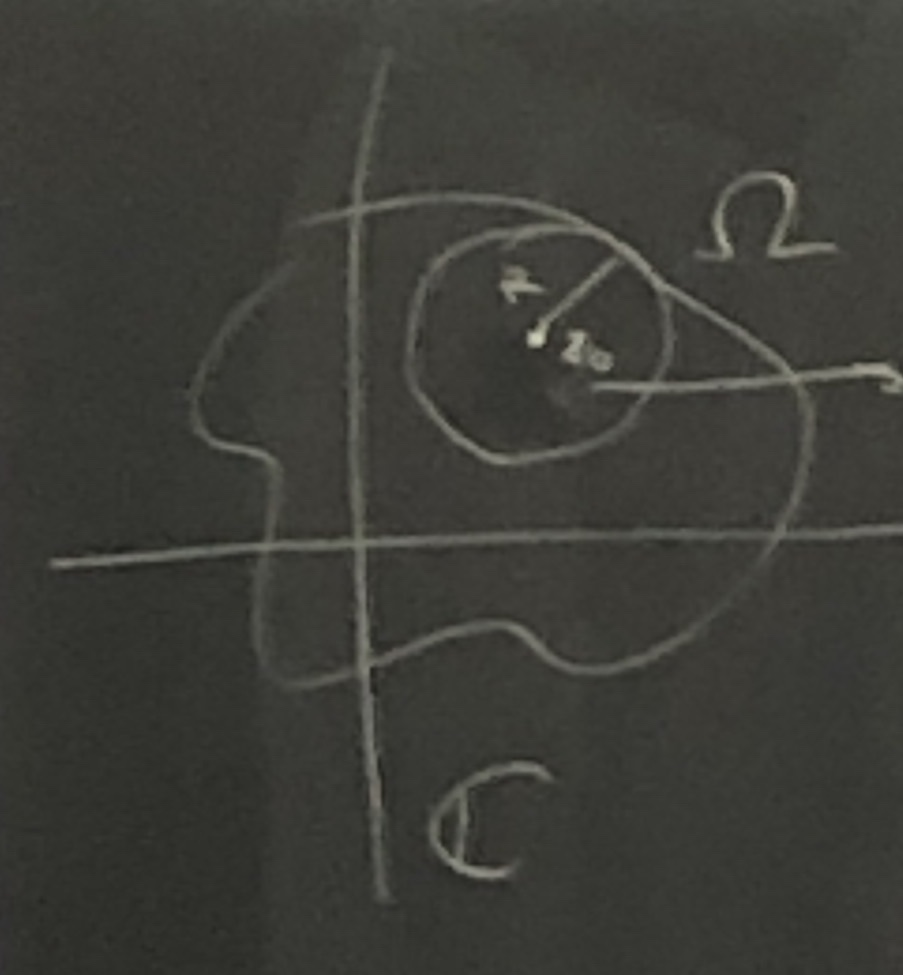
\includegraphics[scale=0.25]{ra_conv_ball}
\caption{If \(B_R(z_0)\) fits in \(\Omega\) then the Taylor series converges to \(f\) at least on \(B_R(z_0)\). See Theorem \ref{ra.thm.taylor.series.520}.}
\label{ra_conv_ball_fig}
\end{center}
\end{figure}


\end{theorem}



Pugh (end of section 4.2): compare \(1/(1+x^2)\) to \(e^x\). Think about \(1/(1+z^2)\) in complex numbers; it blows up at \(z = \pm i\). So the largest possible radius of convergence in the complex plane is \(1\). That's basically why the radius of convergence of the Taylor series of \(1/(1+x^2)\) centered at 0 is only 1. 

\subsection{Compactness and Equicontinuity in \(C^0\) (Section 4.3 of \citet{pugh2015real})}

Recall: \(X\) set, \(Y\) complete metric space, then \(C_b(X,Y)\) is complete (Corollary \ref{ra.pugh.thm.4.3}). If \(X\) is a metric space, then \(C^0(X,Y)\) is complete (Corollary \ref{ra.thm.complete.c0}). How about if \(Y\) is compact? Is \(C^0(X,Y)\) compact?

\begin{example}

\(X = [n]\) with discrete metric. \(C^0([n], \mathbb{R}) \approx  \mathbb{R}^n\) with \(\ell^1\) metric, \(d(x,y) = \max|x_i - y_i|\). Then \(C^0([n], [-1,1]) \approx [-1, 1]^n\) with \(\ell^1\) metric.

In this case, \([-1,1]^n\) is compact in the usual metric, so compact here.

But: now let \(X := \mathbb{N}\). Consider \((C^0(\mathbb{N}, [-1,1]), d_\infty)\). Is this compact? No. Counterexample: \(f_n(x) = \begin{cases}1, & x =n \\ 0, & x \neq n\end{cases}\). Exercise; there does not exist a uniformly convergent subsequence for this sequence. So \(C^0(\mathbb{N}, [-1,1])\) is not compact. 

\end{example}

One way to think about this: \(C^0(\mathbb{N}, [-1,1])\) is the closed unit ball in \(C^0(\mathbb{N}, \mathbb{R})\). This is a Banach space under \(\lVert \cdot \rVert_\infty\). This is an infinite dimensional vector space. In a finite-dimensional normed vector space, can show that the closed unit ball is compact. But in infinite dimensional vector spaces that usually goes wrong. 

\begin{definition}[\textbf{Equicontinuity; definition 7.22 in \citet{rudin1976principles}, p.165 of pdf, p.156 of book}]

Let \((X, d), (Y, d')\) be metric spaces. Let \(\mathcal{E}\) be a set of functions from \(X\) to \(Y\). \(\mathcal{E}\) is called \textbf{equicontinuous} if for every \(\epsilon > 0\) there exists \(\delta > 0\) depending only on \(\epsilon\) such that for all \(x, x' \in X\) with \(d(x, x') < \delta\) and for all \(f \in \mathcal{E}\) we have \(d'(f(x), f(x')) < \epsilon\). 

\end{definition}

Note: if \(\mathcal{E}\) is equicontinuous and \( f \in \mathcal{E}\) then \(f\) is uniformly continuous. So being equicontinuous is like being uniformly continuous together. 

Can also formulate ``pointwise equicontinuity:" \(\delta\) can depend on a fixed point \(x_0\) (but cannot depend on \(f \in \mathcal{E}\)).

Sequence of functions \((f_n)_{n=1}^\infty\): can take \(\mathcal{E} = \{f_n: n \geq 1 \}\) and ask if \(\mathcal{E}\) is equicontinuous. Write explicitly what this means:

\begin{definition}

 \(f_n: X \to Y\), with \(X, Y\) metric spaces. \((f_n)_{n=1}^\infty\) is an equicontinuous sequence if for every \(\epsilon > 0\) there exists \(\delta > 0\) such that if \(x, x' \in X\), \(d(x, x') < \delta\) then for every \(n \in \mathbb{N}\), \(d'(f_n(x), f_n(x')) < \epsilon\). 

\end{definition}

Last time: finished Section 4.2 of \citet{pugh2015real}. Learned a trick for determining the radius of convergence of an infinite series geometrically if you go to \(\mathbb{C}\). 

Next we discussed that in infinite dimensional normed vector spaces, the closed unit ball might not be compact. (In fact, the closed unit ball is compact if and only if it is finite-dimensional. Recall: definition of dimension is the number of elements in a basis for the space.) Next we discussed how to ensure compactness of subsets of \(C^0(X, \mathbb{R})\) where \(X\) is a compact metric space. One way is if the space is totally bounded and complete, but this is harder than applying Heine-Borel (Theorem 2.33 in \citet{pugh2015real}, Theorem \ref{ra.heine-borel.thm} in these notes) to the equivalent question for subsets of \(\mathbb{R}^m\), where you just need to show the set is closed and bounded. Can we get an analogous result to Heine-Borel for subsets of \(C^0(X, \mathbb{R})\) (where \(X\) is a compact metric space)? Yes: it turns out \(\mathcal{E} \subset C^0(X, \mathbb{R})\) is compact if and only if it is closed, bounded, and equicontinuous. (We will show this in Theorem \ref{ra.thm.gen.heine.borel.fnc}.)

\begin{example}[\textbf{Non-example: sequence of functions that is not equicontinuous}]

Let \(X = [0,1]\) and \(Y = \mathbb{R}\). Let \(f_n(x) = x^n\). We will show that the set \(\{f_n\}_{n=1}^\infty\) is not equicontinuous. Assume there exists \(\delta \in( 0, 1)\) such that if \(s, t \in [0,1]\) and \(|s -t | < \delta\) and \(n \geq 1\), then \(|f_n(s) -f_n(t)| <1/2\) (that is, let \(\epsilon = 1/2\)).  We know \(\lim_{n \to \infty} (1 - \delta/2)^n = 0\), so there exists \(n^*\) with \((1 -\delta/2)^{n^*} < 1/2\). Then

\[
\left| f_{n^*}(1 - \delta/2) -  f_{n^*}(1) \right| = \left| \underbrace{(1 - \delta/2)^{n^*}}_{< 1/2} -  \underbrace{1^{n^*}}_{=1} \right| > \frac{1}{2},
\]

contradiction. Therefore \(\{f_n\}_{n=1}^\infty\) is not equicontinuous. 

Note: these functions are a sequence of functions in the closed unit ball of \((C^0([0,1], \mathbb{R}), \lVert \cdot \rVert_\infty)\) with no convergent subsequence. (This is true because if the limit existed it would be a uniform limit since we are using the \( \lVert \cdot \rVert_\infty\) norm, and then the uniform limit would equal the pointwise limit since each of the individual functions are continuous. But the pointwise limit is not continuous.)

\end{example}

From this example we get an intuition that equicontinuity is related to the slopes of functions in the subset being bounded in some sense. How do we ensure equicontinuity? We can do it if we can bound the slopes of the functions, in the sense of the following definition.

\begin{definition}\label{ra.def.lipschitz}

Let \((X, d)\) and \((Y, d')\) be metric spaces. Let \(f: X \to Y\). Then 

\begin{enumerate}

\item \(M \in \mathbb{R}\) is a \textbf{Lipschitz constant} for \(f\) if 

\[
\forall x, x' \in X, \text{ we have } d'(f(x), f(x')) \leq M  \cdot d(x, x').
\]

\item \(M \in \mathbb{R}\) is a \textbf{uniform Lipschitz constant} for a set of functions \(\mathcal{E} \subseteq C^0(X, Y)\) if 

\[
\forall f \in \mathcal{E} \text{ and } \forall x, x' \in X \text{ we have } d'(f(x), f(x')) \leq M \cdot d(x, x').
\]

\end{enumerate}

\end{definition}

Think of \(M\) as a ``global steepness bound" for \(f\). Note that \(f\) having a Lipschitz constant \(M\) (that is, \(f\) is \textbf{Lipschitz continuous}) implies that \(f\) is uniformly continuous. (Proof: exercise. Hint: given \(\epsilon\), take \(\delta = \epsilon/M\).)



\begin{proposition}\label{ra.prop.lipschitz.equi}

If a uniform Lipschitz constant \(M\) exists for a \(\mathcal{E} \subset C^0(X, Y)\), then \(\mathcal{E}\) is equicontinuous.

\end{proposition}

\begin{proof}

Let \(\epsilon >0\). Take \(\delta := \epsilon/M\). If \(x, x' \in X\), \(d(x, x') < \delta\), and \(f \in \mathcal{E}\), then 

\[
d'(f(x), f(x')) \leq M d(x, x') < M\cdot  \frac{\epsilon}{M} = \epsilon.
\]

\end{proof}

This makes sense when \(X, Y\) are metric spaces. Lipschitz constants are global bounds on steepness. What about local bounds?

\begin{corollary}

If \(\mathcal{E}\) is a set of differentiable functions from \([a,b]\) to \(\mathbb{R}\) (or \(\mathbb{C}\)) and there exists \(M \in \mathbb{R}\) such that \(|f'(\theta)| \leq M\) for all \(f \in \mathcal{E}\) and for all \(\theta \in [a,b]\), then \(\mathcal{E}\) is equicontinuous.

\end{corollary}

\begin{proof}

By the Mean Value Theorem, \(M\) is a uniform Lipschitz constant for \(\mathcal{E}\). This implies that \(\mathcal{E}\) is equicontinuous. (Details: exercise.)

\end{proof}

\begin{example}[\textbf{Sanity check}] Let \(X = [0,1]\). Let \(Y = \mathbb{R}\). Let \(f_n(x) = x^n\). Based on what we've just done, there shouldn't be a uniform bound on \(|f_n'(\theta)|\) for all \(n, \theta\), because if there were, this would imply equicontinuity. 

Let's check: we have \(f_n'(x) = nx^{n-1}\). Note that \(\lVert f_n' \rVert_\infty = n\). Question: does there exist any \(M\) such that \(\lVert f_n' \rVert_\infty \leq M\) for all \(n\)? Of course not: there is no \(M\) such that for all \(n \in \mathbb{N}\), \(n \leq M\). So everything is consistent.

\end{example}




A couple more remarks: Generalized Heine-Borel: we will show in Theorem \ref{ra.thm.gen.heine.borel.fnc} (Theorem 4.18 in \citet{pugh2015real}) that \(\mathcal{E} \subset C^0(X, \mathbb{R})\) with \(X\) is compact if and only if \(\mathcal{E}\) is closed, bounded, and equicontinuous. Is this really a generalization---does it recover the usual Heine-Borel theorem (Theorem 2.33 in \citet{pugh2015real}, Theorem \ref{ra.heine-borel.thm} in these notes)? Yes. Consider \(X = \{1, \ldots,n \}\). Any subset of \(C^0(\{1, \ldots, n\}, \mathbb{R})\) is equicontinuous. (We can think of the set \(C^0(\{1, \ldots, n\}, \mathbb{R})\) as being an alternative way of expressing \(\mathbb{R}^n\) itself.) Thus, \(\mathcal{E} \subset \mathbb{R}^n\) is compact if and only if \(\mathcal{E}\) is closed and bounded. That is, Heine-Borel can be thought of as an application of Theorem \ref{ra.thm.gen.heine.borel.fnc} in the special case of the set \(C^0(\{1, \ldots, n\}, \mathbb{R})\).


%
%
%
%
%
%
%

\begin{proposition}[\textbf{Math 425b Homework 5}]\label{ra.425b.hw5.finite.set}

Let \(\{f_1, \ldots, f_k\}\) be a finite set of uniformly continuous functions from \(X\) to \(Y\), where \((X,d)\) and \((Y,d')\) are metric spaces. Then \(\{f_1, \ldots, f_k\}\) is equicontinuous.

\end{proposition}


\begin{proof}

Let \(\epsilon > 0\). Because all the \(f_i\) are continuous, for every \(i \in \{1, \ldots, k\}\) there exists \(\delta_i\) such that for all \(x \in X\), \(d(x, x') < \delta_i \implies d'(f_i(x), f_i(x')) < \epsilon\). Let \(\delta := \min_{i \in \{1, \ldots, k\}} \delta_i\). Then for all \(i \in \{1, \ldots, k\}\), \((d(x, x') < \delta_i \implies d'(f_i(x), f_i(x')) < \epsilon\). 

\end{proof}


\begin{proposition}[\textbf{Math 425b Homework 5}]\label{ra.425b.hw5.3}

Let \(\{f_\alpha\}_{\alpha \in A}\) be an equicontinuous set of functions from \(X\) to \(Y\), and let \(g\) be a uniformly continuous function from \(Y\) to \(Z\), where \((X, d_X), (Y, d_Y)\), and \((Z, d_Z)\) are metric spaces. Then the set of functions \(\{g \circ f_\alpha\}_{\alpha \in A}\) is equicontinuous.

\end{proposition}


\begin{proof}

Let \(\epsilon > 0\). Because \(g\) is uniformly continuous, there exists \(\delta > 0\) such that for any \(y, y' \in Y\), \(d_Y(y, y') < \delta \implies d_Z(g(y), g(y')) < \epsilon\). Because \(\{f_\alpha\}_{\alpha \in A}\) is equicontinuous, there exists an \(\eta > 0\) such that for all \(\alpha \in A\), \(d_X(x, x') < \eta \implies d_Y( f_\alpha(x), f_\alpha(x')) < \delta\). Therefore for all \(\alpha \in A\), \(d_X(x, x') < \eta \implies d_Z(g(f_\alpha(x)), g(f_\alpha(x'))) < \epsilon\), so \(\{g \circ f_\alpha\}_{\alpha \in A}\) is equicontinuous.

\end{proof}

\begin{proposition}[\textbf{Math 425b Homework 5; Exercise 4.8 in \citet{pugh2015real}}]\label{ra.425b.hw5.5}

The sequence of functions \(f_n: \mathbb{R} \to \mathbb{R}\) defined by

\[
f_n(x) = \cos(n +x) + \log \left( 1 + \frac{1}{\sqrt{n+2}} \sin^2(n^nx) \right)
\]

is equicontinuous.

\end{proposition}

\begin{proof}

First we will show that the sequence \(g_n(x) =  \frac{1}{\sqrt{n+2}} \sin^2(n^nx) \) is equicontinuous. Let \(\epsilon > 0\), and let \(N  := \left\lceil 4\epsilon^{-2} - 2 \right\rceil + 1\) so that \((n+2)^{-1/2} < \epsilon/2\) for all \(n \geq N\). By Proposition \ref{ra.425b.hw5.finite.set}, the functions \(\{f_1, \ldots, f_{N-1}\}\) are equicontinuous; that is, there exists \(\delta > 0\) such that for all \(x \in \mathbb{R}\) \(|x - x'| < \delta \implies |g_n(x) - g_n(x')| < \epsilon\) for all \(n \in \{1, \ldots, N-1\}\). Observe that for all \(n \geq N\)

\[
g_n(x) = \frac{\sin^2(n^n x)}{\sqrt{n+2}} < \frac{\epsilon}{2} \cdot \sin^2(n^n x) \leq \frac{\epsilon}{2}
\]

for all \(x \in \mathbb{R}\) since \(\sin^2( x) \in [0,1]\) for all \(x \in \mathbb{R}\). Therefore for all \(n \geq N\) and all \(x, x' \in \mathbb{R}\) it holds that

\[
 |g_n(x) - g_n(x')| <  \left|\frac{\epsilon}{2} + \frac{\epsilon}{2} \right| = \epsilon.
 \]
 
 In particular, this holds if \(|x - x'| < \delta\), so \((g_n)_{n=1}^\infty\) is equicontinuous. Next we will show that \((\cos(n+x))_{n=1}^\infty\) is an equicontinuous sequence on \([0, 2\pi]\). By Proposition \ref{ra.prop.lipschitz.equi}, a sufficient condition to show this is that there exists \(M \in \mathbb{R}\) such that 

\[
\left| \deriv{}{\theta} \cos(n+x) \right| \leq M  \qquad \forall n \in \{1, 2, \ldots\}, \forall x \in [0, 2\pi].
\]

This follows since

\[
\left| \deriv{}{\theta} \cos(n+x) \right| = | \sin(n + x)| \leq 1 \qquad \forall n \in \mathbb{N}, \forall x \in \mathbb{R}.
\]

Then by the periodicity of \(\cos(\cdot)\), \((\cos(n+x))_{n=1}^\infty\) is an equicontinuous sequence everywhere. 

By the fact that the sum of two equicontinuous sequences is equicontinuous, the result follows if we can show that \(\left( \log \left[ 1 +  \frac{\sin^2(n^n x)}{\sqrt{n+2}} \right] \right)_{n=1}^\infty\) is equicontinuous. We showed above that \(g_n\) is equicontinuous, so since the sum of two equicontinuous sequences is equicontinuous, \(\left( 1 +  \frac{\sin^2(n^n x)}{\sqrt{n+2}} \right)_{n=1}^\infty\) is equicontinuous. By Proposition \ref{ra.425b.hw5.3}, we would be done if \(\log(\cdot)\) were uniformly continuous, but that is not true. However, it holds that 

\[
1 \leq 1 +  \frac{\sin^2(n^n x)}{\sqrt{n+2}} \leq 2 \qquad \forall n \in \mathbb{N},
\]

so by Proposition \ref{ra.425b.hw5.3} it is enough to show that \(\log(\cdot)\) is uniformly continuous on \([1,2]\). 

We claim this is true. As in the proof of Proposition  \ref{ra.prop.lipschitz.equi}, if there exists \(M \in \mathbb{R}\) such that \( \left| \deriv{}{\theta} \log(\theta)  \right| \leq M \) for all \(\theta \in [1,2]\), then by the Mean Value Theorem \(M\) is a uniform Lipschitz constant for \(\log(\cdot)\) on \([1,2]\) and then \(\log(\cdot)\) is uniformly continuous on \([1,2]\). Note that for \(\theta \in [1,2]\),

\[
 \left| \deriv{}{\theta} \log(\theta)  \right| = \frac{1}{\theta} \in \left[ \frac{1}{2}, 1 \right]
\]

so \( \left| \deriv{}{\theta} \log(\theta)  \right| \leq 1 \) for all \(\theta \in [1,2]\) and the result follows.


\end{proof}

\begin{proposition}[\textbf{Math 425b Homework 5; \citet{pugh2015real} Exercise. 4.22}]

A sequence of smooth equicontinuous functions \(f_n: [a,b] \to \mathbb{R}\) does not necessarily have uniformly bounded derivatives.

\end{proposition}

\begin{proof}

Consider \(f_n: [0, 2\pi] \to \mathbb{R}\) defined by 

\[
f_n(x) := \frac{\sin^2(n^n x)}{\sqrt{n+2}} \qquad \forall n \in \mathbb{N}.
\]

Clearly \(f_n \in C^\infty([0,2\pi], \mathbb{R})\) so \(f_n\) is smooth for all \(n \in \mathbb{N}\). We showed in the proof of Proposition \ref{ra.425b.hw5.5} that \((f_n)_{n=1}^\infty\) is equicontinuous. However,

\[
\deriv{}{x} f_n(x) = \frac{2 \sin(n^nx) \cdot n^n }{\sqrt{n+2}} - \frac{1}{2 (n+2)^{3/2}} \cdot \sin^2(n^n x),
\]

which is a sequence that is not uniformly bounded over \(n\) since if \(x = \frac{\pi}{2n^n}\) (so \( \sin(n^nx) = 1\))

\begin{align*}
\lim_{n \to \infty} \deriv{}{x} f_n(x)  & = \lim_{n \to \infty} \left[ \frac{2 \sin(n^n x ) \cdot n^n }{\sqrt{n+2}}  - \frac{1}{2 (n+2)^{3/2}} \cdot \sin^2(n^n x) \right]
\\ & = \lim_{n \to \infty} \left[ \frac{2  \cdot n^n }{\sqrt{n+2}}  - \frac{1}{2 (n+2)^{3/2}}  \right]
\\ & = \infty.
\end{align*}

\end{proof}











%
%
%
%
%
%
%
%

%Next week we will prove the . Unlike \citet{pugh2015real}, we will explicitly split the proof into two parts: the Arzela-Ascoli Propagation Theorem (equivalent to Theorem 4.16 in \citet{pugh2015real}), and the Arzela-Ascoli Theorem. 

Before proving the Arzela-Ascoli Theorem (Theorem 4.14 in \citet{pugh2015real}) we will recall a concept from Math 425a and prove some lemmas.

\begin{definition}[\textbf{Dense metric spaces (see also Definition \ref{ra.defn.dense.2} for a special case)}]\label{ra.defn.dense.1}

Let \((X, d)\) be a metric space. \(A \subset X\) is \textbf{dense} if any of the following equivalent statements hold:

\begin{enumerate}

\item For all \(x \in X\) and all \(\epsilon > 0\), there exists \(a \in A\) with \(d(x,a) < \epsilon\).

\item Each point in \(X\) is the limit of a sequence in \(A\).

\item \(\overline{A} = X\) (where \(\overline{A}\) denotes the closure of \(X\)). 

\end{enumerate}

\end{definition}

\begin{example}

Some examples: \(\mathbb{Q} \subset \mathbb{R}\) is countable and dense. \(\mathbb{Q} \cap [a,b] \subset [a,b]\) is countable and dense.

\end{example}

\begin{lemma}\label{ra.cmpct.count.dens.sset}

If \(X\) is a compact metric space then \(X\) has a countable dense subset \(A\). (That is, \(X\) is \textbf{seperable}.) 

\end{lemma}

\begin{proof}

\(X\) is totally bounded, so there exists a finite subset \(A_n\)  of \(X\) such that

\[
\bigcup_{a \in A_n}  B_{1/n}(a)  = X.
\]

Let \(A := \bigcup_{n \geq 1} A_n\), a countable subset of \(X\). Want to show: \(\overline{A} = X\). Use condition 1 from Definition \ref{ra.defn.dense.1}: if \(x \in X\) and \(\epsilon > 0\), then choose \(n \) sufficiently large such that \(1/n < \epsilon\). Thus there exists \(a \in A_n \subset A\) with \(x \in B_{1/n}(a) \subset B_\epsilon(a)\), so \(d(x, a) < \epsilon\). Thus \(\overline{A} = X\).

\end{proof}

\begin{lemma}[\textbf{Math 425b Homework 5}]\label{ra.lemma.arzela.ascoli}

Let \(X\) be a compact metric space and let \(A = \{a_n\}_{n \geq 1}\) be a countable dense subset of \(X\). Then for any \(\delta > 0\) there exists \(M\) such that for any \(x \in X\) we have \(d(x, a_i) < \delta\) for some \(i\) with \(1 \leq i \leq M\).

\end{lemma}

\begin{proof}

Let \(\delta > 0\). Because \(A = \{a_1, \ldots\}\) is dense in \(X\), \(\bigcup_{i=1}^\infty B_\delta(a_i)\) covers \(X\). Because \(X\) is a compact metric space, by Theorem 2.63 in \citet{pugh2015real}, \(\bigcup_{i=1}^\infty B_\delta(a_i)\) has a finite subcover. That is, there are finitely many points \(x_1, \ldots, x_{M} \in A\) such that 

\[
X \subset \bigcup_{i=1}^M B_\delta(a_i).
\] 

Therefore for some \(i \in \{1, \ldots, M\}\) it holds that \(d(x, a_i) < \delta\).



\end{proof}






\begin{theorem}[\textbf{Arzela-Ascoli Propagation Theorem (Theorem 4.16 in \citet{pugh2015real})}]

Let \(X\) be a compact metric space. Let \(A \subseteq X\) be a countable dense subset of \(X\) (such a set \(A\) is guaranteed to exist by Lemma \ref{ra.cmpct.count.dens.sset}). Let \(Y\) be a complete metric space. Let \((f_n)_{n=1}^\infty\) be an equicontinuous sequence of functions \(X \to Y\). If \((f_n(a))_{n=1}^\infty\) converges as a sequence in \(Y\) for all points \(a \in A\), then \(f_n\) converge uniformly to some \(f\) on \(X\). 

\end{theorem}

\begin{proof}

Let \(\epsilon > 0\). Then equicontinuity implies that for all \(n \in \mathbb{N}\) there exists \(\delta = \delta_\epsilon\) such that \(d(x, x') < \delta \implies d(f_n(x), f_n(x')) < \epsilon/3\) for all \(n \in \mathbb{N}\). Since \(A\) is countable, call its elements \(\{a_1, \ldots, a_n, \ldots\}\). Because \(X\) is compact, Lemma \ref{ra.lemma.arzela.ascoli} guarantees that for some \(J \in \mathbb{N}\), for all \(x \in X\) there exists \(j \in \{n_1, \ldots, n_J\} \subset \{1, 2, \ldots\}\) such that \(d(x, a_j) < \delta\). By the pointwise convergence assumption, for any \(j \in \{n_1, \ldots, n_J\}\), \((f_n(a_j))_{n=1}^\infty\) is convergent in \(Y\). So it is Cauchy, so there exists \(N_j\) such that for all \(n, m \geq N_j\) and for all \(j \in \{n_1, \ldots, n_J\}\) it holds that 

\begin{equation}\label{4.16.cauchy}
d(f_n(a_j), f_m(a_j)) < \epsilon/3.
\end{equation}

Let \(N := \max_{j \in \{n_1, \ldots, n_J\}} \{N_j\}\); this quantity is well-defined since it is the maximum over a finite countable set. Then for any \(n, m \geq N\), for all \(x \in X\) there exists \(a_j\) such that \(d(x, a_j) < \delta\); for this \(a_j\) it holds that

\begin{align*}
d(f_n(x), f_m(x)) \leq  & d(f_n(x), f_n(a_j)) + d(f_n(a_j), f_m(a_j)) + d(f_m(a_j), f_m(x))
\\ < &  \underbrace{\frac{\epsilon}{3}}_{\text{by equicontinuity}} +  \underbrace{\frac{\epsilon}{3}}_{\text{by } (\ref{4.16.cauchy})} +  \underbrace{\frac{\epsilon}{3}}_{\text{by equicontinuity}} 
\\ = & \epsilon.
\end{align*}

Since \(Y\) is complete and \((f_n) \) are uniformly Cauchy, \(f_n\) is uniformly convergent.

\end{proof}

\begin{theorem}[\textbf{Bolzano-Weierstrass Theorem; Theorem 2.31 in \citet{pugh2015real}}]\label{ra.bolzano.weierstrass}

Every bounded sequence in \(\mathbb{R}^m\) has a convergent subsequence.

\end{theorem}

\begin{theorem}[\textbf{Theorem 7.23 in \citet{rudin1976principles}, p.156, p.165 of pdf}]\label{ra.rudin.thm.7.23}

If \((f_n)\) is a pointwise bounded sequence of complex functions on a countable set \(E\), then \((f_n)\) has a subsequence \(f_{n_k}\) such that \((f_{n_k}(x))\) converges for every \(x \in E\).

\end{theorem}

\begin{proof}

Let \((x_i), i \in \{1, 2, \ldots\}\) be the points of \(E\), arranged in a sequence. Since \((f_n(x_1))\) is bounded, by the Bolzano-Weierstrass Theorem (Theorem \ref{ra.bolzano.weierstrass}) there exists a subsequence (which we will denote by \(S_1 = (f_{1,k}) = \{f_{1,1}, f_{1,2}, f_{1,3}, \ldots\}\)) of \((f_n)\) such that \((f_{1,k}(x_1))\) converges as \(k \to \infty\). 

Now consider the sequence \((f_{1,k}(x_2))\). This sequence is also bounded (it is a subsequence of a bounded sequence), so it has its own subsequence \(S_2 = (f_{2,k}) = \{f_{2,1}, f_{2,2}, f_{2,3}, \ldots\}\)) such that \((f_{2,k}(x_2))\) converges as \(k \to \infty\).

We can continue in this way, creating sequences \(S_n\) such that (a) \(S_n\) is a subsequence of \(S_{n-1}\) for \(n \in \{2, 3, 4, \ldots\}\), (b) \((f_{n,k}(x_n))\) converges as \(k \to \infty\), and (c) the order in which the functions appear is the same in each sequence (we only remove functions, so as \(n\) increases functions may move to the left in the sequence but never to the right).

Now go down the diagonal of the array, considering the sequence \(S = \{f_{1,1}, f_{2,2}, f_{3,3}, \ldots\}\). This sequence (except possibly its first \(n-1\) terms) is a subsequence of \(S_n\) for all \(n = 1, 2, 3, \ldots\). Therefore \((f_{n,n}(x_i)\) converges as \(n \to \infty\) for all \(x_i \in E\).

\end{proof}

\begin{theorem}[\textbf{Arzela-Ascoli Theorem (Theorem 7.25 in \citet{rudin1976principles}, p. 158; simliar to Theorem 4.14 in \citet{pugh2015real})}]\label{ra.arzela.ascoli}

Let \(X\) be a compact metric space. Let \((f_n)_{n=1}^\infty\) be a sequence of functions \(f_n: X \to \mathbb{R}\) (or \(\mathbb{C}\)). Assume

\begin{enumerate}

\item \(\{f_n\}\) is equicontinuous, and

\item  \(\{f_n\}\) is pointwise bounded (for all \(x \in X\), there exists \(M_x\) such that for all \(n \in \mathbb{N}\), \(|f_n(x)| \leq M_x\)).

\end{enumerate}

Then

\begin{enumerate}

\item  \(\{f_n\}\) are uniformly bounded (there exists \(M\) such that for all \(n\) and for all \(x\), \(|f_n(x) | \leq M\)), and

\item  \(\{f_n\}\) have a uniform convergent subsequence. 

\end{enumerate}

\end{theorem}

\begin{remark}

This version is a little stronger than the version stated in \citet{pugh2015real}. It's also a traditional version that is not maximally general.

Exercise: \(\{f_n\}\) having a uniform convergent subsequence is equivalent to the sequence \((f_n)_{n=1}^\infty\) being \textbf{relatively compact} (its closure is compact) in \(C^0(X, \mathbb{R})\).
 
 \end{remark}

\begin{proof}

\begin{enumerate}

\item

By equicontinuity there exists \(\delta\) such that for any \(x, x' \in X\) if \(d(x, x') < \delta\) then \(|f_n(x) - f_n(x')| < 1\) for all \(n\). Because \(X\) is a compact metric space, by Theorem 2.63 in \citet{pugh2015real} \(X\) has a finite subcover. That is, we can pick a finite \(J \in \mathbb{N}\) such that \(X \subset \bigcup_{j=1}^J B_\delta(a_j)\). Because \(f_n\) is pointwise bounded by assumption, there exists \(M_j\) such that \(|f_n(a_j)| < M_j\) for all \(n \in \mathbb{N}\). Let \(M := \max_{j \in \{n_1, \ldots, n_J\}} M_j\). Then for all \(x \in X\), 

\[
|f_n(x)| \leq   |f_n(x) - f_n(a_j)| + |f_n(a_j)| <  M + 1 
\]

which is independent of \(x\). Therefore the \(\{f_n\}\) are uniformly bounded.

\item

Let \(A = \{a_1, \ldots, a_n, \ldots\} \subseteq X\) be a dense, countable subset of \(X\) (such a set \(A\) is guaranteed to exist by Lemma \ref{ra.cmpct.count.dens.sset}). By Theorem \ref{ra.rudin.thm.7.23}, \((f_n)\) has a subsequence \((f_{n_i}) = (g_i)\) (for simplicity of notation) such that \((g_i(x))\) converges for every \(x \in A\). We will show that \((g_i)\) converges uniformly on \(X\). Let \(\epsilon >0\). By equicontinuity there exists \(\delta>0\) such that if \(d(x,x') < \delta\) then 

\begin{equation}\label{4.16.conv.again}
|f_n(x) - f_n(x')| < \epsilon/3 \qquad \forall n.
\end{equation}

Because \(A = \{a_1, \ldots\}\) is dense in \(X\), \(\bigcup_{j=1}^\infty B_\delta(a_j)\) covers \(X\). Because \(X\) is compact, by Theorem 2.63 in \citet{pugh2015real} \(\bigcup_{i=1}^\infty B_\delta(a_i)\) has a finite subcover. That is, there are finitely many points \(a_1, \ldots, a_{J} \in A\) such that 

\[
X \subset \bigcup_{j=1}^J B_\delta(a_j).
\] 

Since \((g_i(x))\) converges for every \(x \in A\), there exists \(N \in \mathbb{N}\) such that 

\begin{equation}\label{4.16.cauchy.again}
|g_m(x_j) - g_n(x_j)| < \frac{\epsilon}{3} \qquad  \forall m, n \geq N, \text{ and any } j \in [J].
\end{equation}

 If \(x \in X\), \(x \in B_\delta(x_j)\) for some \(j\), so for every \(i\) there exists some \(j \in [J]\) such that \(|x - x_j| < \delta\) and therefore \(|g_i(x) - g_i(x_j)| < \epsilon/3\). If \(i \geq N\) and \(k \geq N\), it follows that for some \(j \in [J]\)

\[
|g_i(x) - g_k(x)| \leq \underbrace{| g_i(x) - g_i(x_j)|}_{\text{by } (\ref{4.16.conv.again})} + \underbrace{|g_i(x_j) - g_k(x_j)|}_{\text{by } (\ref{4.16.cauchy.again})}  + \underbrace{|g_k(x_j) - g_k(x)|}_{\text{by } (\ref{4.16.conv.again})} < \epsilon.
\]



%
%\item Consider \((f_n(a_i))_{n-1}^\infty\) is a bounded sequence of real numbers. Then by Bolzano-Weierstraus, \((f_n(a_9)) \) has a convergent subsequence. Pick one: there exists \(n_1 < n_2 < n_3 < \ldots\) such that \((f_{n_j}(a_i))_{j=1}^\infty\) converges in \(\mathbb{R}\). Let \(f_{1,j}(x) = f_{n,j}(x)\).  Now \((f_{1,j}(x))_{j=1}^\infty\) is a subsequence of \((f_n)\) with all the same properties as the original sequence plus pointwise convergence on \(a_1\).
%
%Similarly, look at \((f_{1,j}(a_2))_j\); this is also a convergent subsequence. Let 
%
%\[
%\vdots
%\]

\end{enumerate}

\end{proof}

\begin{theorem}[\textbf{Arzela-Ascoli Theorem for functions into compact metric spaces}]\label{ra.arzela.ascolia.cmpct}

Let \(X\) and \(Y\) be compact metric spaces. Then any equicontinuous sequence of functions \(f_n: X \to Y\) has a uniformly convergent subsequence.

\end{theorem}

\begin{proof}

This follows immediately from Theorem \ref{ra.arzela.ascoli}. (Note that the functions must be pointwise bounded since \(X\) and \(Y\) are compact.)

\end{proof}

Now we will discuss some applications of Arzela-Ascoli (Theorem \ref{ra.arzela.ascoli}).

\begin{theorem}[\textbf{Generalized Heine-Borel in a Function Space, Theorem 4.18 in  \citet{pugh2015real}}]\label{ra.thm.gen.heine.borel.fnc}

Let \(X\) be a compact metric space. Let \(\mathcal{E} \subset (C^0(X, \mathbb{R}), \lVert \cdot \rVert_\infty)\). Then \(\mathcal{E}\) is compact if and only if \(\mathcal{E}\) is closed, bounded, and equitcontinuous.

\end{theorem}

\begin{proof}

\(\implies\): Let \(\epsilon > 0\). Suppose \(\mathcal{E}\) is compact. Then by Theorem 2.65 in \citet{pugh2015real} it is closed and totally bounded, so there is a finite covering of \(\mathcal{E}\) by neighborhoods in \(C^0\) having radius \(\epsilon/3\), say \(B_{\epsilon/3}(f_k)\), with \(k \in [n]\). So if \(f \in \mathcal{E}\) then for some \(k\) we have \(f \in B_{\epsilon/3}(f_k)\). Also, by equicontinuity each \(f_k\) is uniformly continuous, so there exists a \(\delta > 0\) such that \(|s-t| < \delta \implies \lVert f_k(s) - f_k(t) \rVert_\infty < \epsilon/3\). Then \(|s-t | < \delta\) implies

\[
|f(s) - f(t)| \leq | f(s) - f_k(s)| + |f_k(s) - f_k(t) | + |f_k(t) - f(t)| < \epsilon/3 + \epsilon/3 + \epsilon/3 = \epsilon.
\]

Therefore \(\mathcal{E}\) is equicontinuous.

\(\impliedby\): Assume that \(\mathcal{E}\) is closed, bounded, and equicontinuous. If \((f_n)\) is a sequence in \(\mathcal{E}\), by the fact that \(\mathcal{E}\) is bounded then \((f_n)\) are uniformly bounded pointwise. Then by Arzela-Ascoli (Theorem \ref{ra.arzela.ascoli}) there exists a subsequence \((f_{n_k})\) that converges uniformly to a limit. Because \(\mathcal{E}\) is closed, the limit lies in \(\mathcal{E}\). Therefore \(\mathcal{E}\) is compact (see Definition \ref{ra.def.compactness}).

% \((f_n)_1^\infty  \subset \mathcal{E}\) then by the fact that \(\mathcal{E}\) is bounded then \((f_n)\) are uniformly bounded pointwise. Moreover, \((f_n)_n\) are also equal. Since \(\mathcal{E}\) is 

\end{proof}


\begin{proposition}[\textbf{Corollary 4.17 in \citet{pugh2015real}}]\label{ra.pugh.cor.4.17}

Suppose \(f_n: [a,b] \to \mathbb{R}\) is a sequence of differentiable \(C^1\) functions whose derivatives are uniformly bounded. If there exists one point \(x_0 \in [a,b]\) such that the sequence \((f_n(x_0))\) is bounded as \(n \to \infty\), then \((f_n)\) has a convergent subsequence such that \(f_n\) converges uniformly to \(f\) on the whole interval \([a,b]\) and \(f' = g\)  \textbf{not sure about this convergence of derivative part}. 


%, where \(f_n \in C^1\). Suppose \(f_n'\) converge uniformly to \(g\). a
\end{proposition}

\begin{proof}

Let \(M\) be a bound for the derivatives \(|f_n'(x)|\), valid for all \(n \in \mathbb{N}\) and all \(x \in [a,b]\). Equicontinuity of \((f_n)\) follows from the Mean Value Theorem:

\[
|s-t| < \delta \implies |f_n(s) - f_n(t)| = |f_n'(\theta)| |s-t| \leq M \delta
\]

for some \(\theta\) between \(s\) and \(t\). Thus given \(\epsilon > 0\) the choice \(\delta = \epsilon/(M+1)\) shows that \((f_n)\) is equicontinuous: in particular, for all \(n \in \mathbb{N}\) it holds that

\[
|s-t| < \frac{\epsilon}{M+1} \implies |f_n(s) - f_n(t)| = |f_n'(\theta)| |s-t| \leq M \cdot  \frac{\epsilon}{M+1} < \epsilon.
\]

Let \(C\) be a bound for \(|f_n(x_0)|\), valid for all \(n \in \mathbb{N}\) (by assumption). Then

\[
|f_n(x)| \leq | f_n(x) - f_n(x_0)| + |f_n(x_0)| \leq M |x - x_0| + C \leq M|b-a| + C
\]

shows that the sequence \((f_n)\) is bounded in \(C^0\). Then by Arzela-Ascoli (Theorem \ref{ra.arzela.ascoli}) there exists a subsequence \((f_{n_k})\) that converges uniformly to a limit on the whole interval. \textbf{not sure about convergence of derivative}

\end{proof}



\begin{proposition}[\textbf{Math 425b Homework 5; \citet{pugh2015real} Exercise. 4.23 (a) and (b)}]

Let \((M,d)\) be a compact metric space, and let \((i_n)\) be a sequence of isometries \(i_n: M \to M\). Then there exists a subsequence \(i_{n_k}\) that converges to an isometry \(i\) as \(k \to \infty\), and the space of self-isometries of \(M\) is compact.

\end{proposition}

\begin{proof}

Let \(\epsilon > 0\). Then for all \(n \in \mathbb{N}\) and for all \(m, m' \in M\)

\[
d(m, m') < \epsilon \implies d(i_n(m), i_n(m')) = d(m, m') < \epsilon,
\]

so \((i_n)_{n=1}^\infty\) is equicontinuous. Then by Theorem \ref{ra.arzela.ascolia.cmpct}, \((i_n)_{n=1}^\infty\) has a subsequence  \((i_{n_1}, i_{n_2}, \ldots)\) converging uniformly to a limit \(i: M \to M\).

It remains to show that this limit is an isometry. By the definition of continuity in Section 2.2 of \citet{pugh2015real}, the limit of a continuous function of convergent sequences is the function of the limits of the sequences. Metrics are continuous by Theorem 2.20 in \citet{pugh2015real}. So a subsequence \\ \((d(i_{n_1}(m), i_{n_1}(m')), d(i_{n_2}(m), i_{n_2}(m')), \ldots)\) converges to \(d(i(m), i(m'))\). The sequence itself can be written

\[
(d(i_{n_1}(m), i_{n_1}(m')), d(i_{n_2}(m), i_{n_2}(m'), \ldots) = (d(m, m'), d(m, m'), \ldots)
\]

since each \(i_n\) is an isometry. This constant sequence converges to \(d(m, m')\), so \(d(i(m), i(m')) = d(m, m')\) and \(i\) is an isometry.

Because we have shown that every sequence of isometries \((i_n)\) from \(M\) to \(M\) has a subsequence that converges to an isometry from \(M\) to \(M\), we have shown that the space of self-isometries of \(M\) is compact.


\end{proof}


\subsection{Uniform Approximation in \(C^0\) (Section 4.4 of \citet{pugh2015real})}

\begin{definition}[\textbf{Dense sets of functions; special case of Definition \ref{ra.defn.dense.1}}]\label{ra.defn.dense.2}

Let \(X\) be a set of functions. \(X\) is \textbf{dense} in \(C^0([a,b], \mathbb{R})\) if for each \(f \in  C^0\) and each \(\epsilon >0\) there exists a function \(p \in X\) such that for all \(x \in [a,b]\), \(|f(x) - p(x)| < \epsilon\). 

\end{definition}




\begin{theorem}[\textbf{Weierstrass Approximation Theorem; Thereom 4.19 in \citet{pugh2015real}}]\label{ra.thm.weierstrass.approx}

The set of polynomials is dense in \(C^0([a,b], \mathbb{R})\).

(Alternatively: Let \(f \in C^0([0,1], \mathbb{R})\) (or \(C^0([0,1], \mathbb{C})\)). Then the polynomials \(p_n(x) = \sum_{k=0}^n f(k/n) f_k(x)\) converge uniformly to \(f\) on \([0,1]\).)

\end{theorem}

\begin{remark}

See p. 229 of \citet{pugh2015real} (p. 239 of pdf), Proof \(\# 1\).

We will sketch the proof that the result generalizes from \([0,1]\) to \([a,b]\). We have isomorphisms (mappings between two structures of the same type that can be reversed by inverse mappings; see Definition \ref{ra.def.isomorphism}) of \(\mathbb{R}\)-vector spaces \(C^0([0,1],\mathbb{R}) \) to and from \(C^0([a,b],\mathbb{R})\). Suppose we have \(f \in C^0([0,1],\mathbb{R})\); we can send it to \(x \mapsto f([x-a]/[b-a])\) in  \(C^0([a,b],\mathbb{R})\). Conversely, we can send a function \(g \in C^0([a,b],\mathbb{R})\) to \(C^0([0,1],\mathbb{R}) \) via the map \(x \mapsto g(a + x[b-a])\). It can be checked that these isomorphisms are linear, compose to the identity in either order, and preserve \(\lVert \cdot \rVert_\infty\). They also send polynomials to polynomials.
%
%Let \(X = [a,b]\). Consider \(C^0([0,1], \mathbb{R})\). Let \(f:[0,1] \to \mathbb{R}\) be continuous. The values of \(f\) are given with probability \(x\), \(f(x)\), like an unfair coin model. 

\end{remark}

First we will show a lemma.

\begin{lemma}\label{ra.weierstrass.approx.lemma.max}

\(x(1-x) \leq 1/4\) for all \(x \in \mathbb{R}\).

\end{lemma}

\begin{proof}

\(f(x) = x(1-x) = -x^2 + x\) is differentiable; \(f'(x) = -2x + 1 =0 \iff x = 1/2\). We see that \(f'\) is continuous on \(\mathbb{R}\) and \(f'(x) > 0 \) for \(x \in (-\infty, 1/2)\) and \(f'(x) < 0 \) for \(x \in (1/2, \infty)\), so \(f(x)\) has a global maximum at \(x=1/2\); that is, \(x(1-x) \leq f(1/2) = 1/2(1-1/2) = 1/4\) for all \(x \in \mathbb{R}\).

\end{proof}

\begin{proof}[Proof of Weierstrass Approximation Theorem (Theorem \ref{ra.thm.weierstrass.approx})]

For a given \(n \geq 1\) and for \(k \in \{0, \ldots, n\}\), let \(r_k\) be the Bernstein basis polynomial

\[
r_k(x) = \binom{n}{k}x^k (1-x)^{n-k}.
\]

Define

\[
p_n(x) := \sum_{k=0}^n f(k/n) r_k(x).
\]

We want to show that the polynomial functions \(p_n\) converge uniformly to \(f\) on \([0,1]\). Let \(\epsilon > 0\). Note that \(f\) is uniformly continuous and bounded because it is a continuous function on a compact set. So, there exists \(\delta > 0\) such that for any \(x, y \in [0,1]\),

\begin{equation}\label{ra.weierstrass.approx.unif.cont}
|x - y| < \delta \implies | f(x) - f(y)| < \epsilon/2,
\end{equation}

 and there exists \(M \in (0, \infty)\) such that 
 
\begin{equation}\label{ra.weierstrass.approx.bound}
 |f(x)| \leq M
 \end{equation}
 
  for all \(x \in [0,1]\). Let \(N \geq M/(\epsilon \delta^2)\). We want to show that for any \(n \geq N\), \(|p_n(x) - f(x)| < \epsilon\) for all \(x \in [0,1]\).

Fix \(x \in [0,1]\). Since \(\sum_{k=0}^n r_k(x) = 1\), we have \(f(x) = f(x) \sum_{k=0}^n r_k(x)  = \sum_{k=0}^n  f(x)r_k(x) \). Then

\begin{equation}\label{ra.weierstrass.sum.bound}
\left|  p_n(x) - f(x) \right| = \left|   \sum_{k=0}^n f(k/n) r_k(x) - \sum_{k=0}^n  f(x)r_k(x) \right| = \left|   \sum_{k=0}^n \left[ f(k/n) - f(x) \right] r_k(x) \right|.
\end{equation}

Let \(K_1 := \left\{k \in \{0, \ldots,n \} : \left| k/n - x \right| < \delta \right\}\), and let \(K_2 := \{0, \ldots, n\} \setminus K_1\). Observe that for all \(k \in K_1\), \(|f(k/n) - f(x)| < \epsilon/2\) by (\ref{ra.weierstrass.approx.unif.cont}), so

\begin{equation}\label{ra.weierstrass.approx.k1.bound}
 \left|   \sum_{k \in K_1} \left[ f(k/n) - f(x) \right] r_k(x) \right| \leq   \sum_{k =0}^n  \left|   \left[ f(k/n) - f(x) \right] r_k(x) \right| < \sum_{k=0}^n \frac{\epsilon}{2} | r_k(x)| = \frac{\epsilon}{2}  \sum_{k=0}^n r_k(x ) = \frac{\epsilon}{2}
\end{equation}

where we used \(r_k(x ) \geq 0\) for all \(k\). Next, by (\ref{ra.weierstrass.approx.bound}) \(| f(k/n) - f(x) | \leq | f(k/n) | + |f(x)| \leq 2M \leq  2\epsilon \delta^2n \) (using the definition of \(N\) and \(n \geq N\)), so

\[
 \left|   \sum_{k \in K_2} \left[ f(k/n) - f(x) \right] r_k(x) \right|  \leq   \sum_{k \in K_2}   2\epsilon \delta^2nr_k(x).
 \]


Since \(k \in K_2 \iff \left| k/n - x \right| \geq \delta \iff \left| k -n x \right| \geq \delta n \implies (k-nx)^2 \geq (n \delta)^2\), we have (using \(\sum_{k =1}^n (k -nx)^2 r_k(x) = nx(1-x)\))

\[
\sum_{k \in K_2}   2\epsilon \delta^2nr_k(x) = \frac{2 \epsilon}{n} \sum_{k \in K_2} (n \delta)^2 r_k(x) \leq \frac{2 \epsilon}{n} \sum_{k =1}^n (k -nx)^2 r_k(x) = \frac{2 \epsilon}{n} nx(1-x) \leq 2 \epsilon  \cdot \frac{1}{4} = \frac{\epsilon}{2}
\]

where we applied Lemma \ref{ra.weierstrass.approx.lemma.max} in the last step, yielding

\begin{equation}\label{ra.weierstrass.approx.k2.bound}
 \left|   \sum_{k \in K_2} \left[ f(k/n) - f(x) \right] r_k(x) \right|  \leq \frac{\epsilon}{2}.
\end{equation}

Therefore using (\ref{ra.weierstrass.approx.k1.bound}) and (\ref{ra.weierstrass.approx.k2.bound}) we can write (\ref{ra.weierstrass.sum.bound}) as 

\begin{align*}
\left|  p_n(x) - f(x) \right| & = \left| \sum_{k \in K_1} \left[ f(k/n) - f(x) \right] r_k(x) +  \sum_{k \in K_2} \left[ f(k/n) - f(x) \right] r_k(x)\right|
\\ & \leq \left| \sum_{k \in K_1} \left[ f(k/n) - f(x) \right] r_k(x)\right| +  \left| \sum_{k \in K_2} \left[ f(k/n) - f(x) \right] r_k(x)\right|
\\ & < \frac{\epsilon}{2} + \frac{\epsilon}{2}
\\ & = \epsilon.
\end{align*}

\end{proof}

\begin{definition}[\textbf{Definition 7.28 in \citet{rudin1976principles}, p. 170 of pdf, p.161}]

A family \(A\) of complex functions defined on a set \(X\) is a \textbf{function algebra} if \(A\) is closed under addition, multiplication, and scalar multiplication (and does not necessarily include a multiplicative identity). That is, if \(f, g \in A\) and \(c \in \mathbb{C}\), then \(f + g \in A\), \(fg \in A\), and \(cf \in A\). (We also consider algebras of real functions; in this case, the conditions only must hold for all \(c \in \mathbb{R}\).)

If \(A\) has the property that \(f \in A\) whenever \(f_n \in A\) for \(n \in \mathbb{N}\) and \(f_n\) converges uniformly to \(f\) on \(X\), then \(A\) is said to be \textbf{uniformly closed.}

Let \(B\) be the set of all functions that are limits of uniformly convergent sequences of members of \(A\). Then \(B\) is called the \textbf{uniform closure} of \(A\).

In-class definition: a ``non-unital subalgebra of \(C^0(X, \mathbb{R}\)". Also an \(\mathbb{R}\)-algebra: a ring (see Definition \ref{abs.alg.def.ring}) that's also an \(\mathbb{R}\) vector space; structures are compatible. e.g. \(C^0(X, \mathbb{R})\) is an \(\mathbb{R}\)-algebra. A sub-algebra is closed under addition, scalar multiplication, and ring multiplication, and contains a scalar multiplicative identity. A non-unital sub-algebra is the same but it might not contain a multiplicative identity. (Note that the multplicative identity for \(C^0(X, \mathbb{R})\) is the constant function \(f(x) = 1\).)

\end{definition}

\begin{example}

The set of all polynomials is an algebra. The Weierstrass Approximation Theorem may be stated by saying that the set of continuous functions on \([a,b]\) is the uniform closure of the set of polynomials on \([a,b]\).

\end{example}

\begin{definition}[\textbf{Definition 7.30 in \citet{rudin1976principles}, p. 171 of pdf, p.162}]

Let \(A\) be a family of functions on a set \(X\). \(A\) \textbf{vanishes nowhere} if \(\forall x \in X\) there exists \( f \in A\) with \(f(x) \neq 0.\) (That is, there is no \(x \in X\) with \(f(x) = 0\) for all \(f \in A\).)

\end{definition}

\begin{definition}[\textbf{Definition 7.30 in \citet{rudin1976principles}, p. 171 of pdf, p.162}]

Let \(A\) be a family of functions on a set \(X\). \(A\) \textbf{separates points} on \(X\) if \(\forall x \neq x' \in X\) there exists \( f \in A\) with \(f(x) \neq f(x').\)

\end{definition}

\begin{example}

The algebra of all polynomials in one variable clearly vanishes nowhere and separates points on \(\mathbb{R}\). An example of an algebra that does not separate points is the set of all even polynomials, say on \([-1,1]\) since \(f(-x) = f(x)\) for every even function \(f\).


\end{example}

\begin{theorem}[\textbf{Stone-Weierstrass Theorem (Theorem 4.20 in \citet{pugh2015real}, Theorem 7.32 in \citet{rudin1976principles}, p. 171 of pdf, p.162}]\label{ra.stone.weierstrass}

Let \(X\) be a compact metric space. Let \(A \subset C^0(X, \mathbb{R})\) or \(C^0(X, \mathbb{C})\). Then if \(A\) is a function algebra that vanishes nowhere in \(X\) and \(A\) separates points on \(X\), then \(A\) is dense in \((C^0(X, \mathbb{R}), \lVert \cdot \rVert_\infty)\).

Equivalent conclusion: \(\overline{A} = C^0(X, \mathbb{R})\) in uniform metric. That is, the uniform closure \(B\) of \(A\) consists of all real continuous functions on \(X\).

\end{theorem}

\begin{remark}

The Weierstrass Approximation Theorem (Theorem \ref{ra.thm.weierstrass.approx}) is a special case of the Stone-Weierstrass Theorem.

\end{remark}

\begin{theorem}[\textbf{Complex Stone-Weierstrass Theorem; similar to Theorem 7.33 in \citet{rudin1976principles}, p. 174 of pdf, p.165}]\label{ra.stone.weierstrass.cmpx}

If \(A \subset C^0(X, \mathbb{C})\) is a function algebra that is closed under complex conjugation, \(A\) vanishes nowhere, and \(A\) separates points, then \(A\) is dense in \((C^0(X, \mathbb{C}), \lVert \cdot \rVert_\infty)\) (that is, \(\overline{A} = C^0(X, \mathbb{C})\).

\end{theorem}

\begin{remark}
Why is the complex conjugate assumption needed? Let \(X := \{ |z| \leq 1 | z \in \mathbb{C}\}\). Note that \(X\) is compact. Let \(A\) be the space of complex polynomials; that is, \(A = \operatorname{span}_{\mathbb{C}}(1, z, z^2, \ldots)\). It can be shown that \(A\) is a function algebra, separates points, and vanishes nowhere. Let \(f(z) = \overline{z}\); this is not holomorphic. If \(p_n \in A\) and \(p_n\) converges uniformly to \(f\) on \(X\), then \(p_n\) converges uniformly to \(f\) on \(\{|z | < 1. | z \in \mathbb{C}\}\). Thus \(p_n\) (which are holomorphic) converges uniformly to \(f\) on any compact \(K \subset \{|z| = 1 \mid z \in \mathbb{C}\}\). This implies (by Theorem \ref{ra.complex.analysis.thm.diff.power.series}) that \(f\) is holomorphic, contradiction. So we need \(A\) to be closed under complex conjugation.

\end{remark}

Now we will prove Theorem \ref{ra.stone.weierstrass}. We will need to use the Weierstrass Approximation Theorem (Theorem \ref{ra.thm.weierstrass.approx}) for \(f(x) = |x|\) on \([-1,1]\) (could prove what we need direcdtly for this function, but we might as well use the result since we have it). We will show some lemmas first

\begin{lemma}[\textbf{Lemma 4.22 in \citet{pugh2015real}; Similar to Theorem 7.29 in \citet{rudin1976principles}, p. 170 of pdf, p.161}]\label{ra.rudin.7.29.lem}

If \(X\) is compact and \(A \subset C^0(X, \mathbb{R})\) is a function algebra, then so is its closure \(\overline{A}\).

\end{lemma}

\begin{proof}

We will show \(\overline{A}\) is closed under addition, scalar multiplication, and function multiplication. (We will prove that it is true for addition; the other two cases are similar.) Let \(f, g \in \overline{A}\). We have \(f_n \in A\) with \(f_n \) converging uniformly to \(f\) and \(g_n \in A\) with \(g_n\) converging uniformly to \(g\). \(A\) is closed under addition by assumption, so \(f_n + g_n \in A\). The limits of nets are linear (exercise), so we have that \(f_n + g_n\) converges uniformly to \(f + g\). Thus \(f+ g\) is a uniform limit of elements of \(A\), so \(f+g \in \overline{A}\). 

The proof of closure under scalar multiplication and function multiplication are similar.

\end{proof}

\begin{lemma}\label{ra.stone.lem.class}

Let \(f \in C^0([a,b], \mathbb{R})\) and let \(x_0 \in [a,b]\) with \(f(x_0) = 0\). Given \(\epsilon > 0\), there exists a polynomial \(p\) on \([a,b]\) with \(p(x_0) = 0\) and \(|f(x) - p(x) | < \epsilon\) for all \(x \in [a,b]\).

\end{lemma}

\begin{proof}

Given \(\epsilon > 0\), choose a polynomial \(	q\) such that \(|f(x) - q(x)| < \epsilon/2\) for all \(x \in [a,b]\). \(q\) might not vanish at \(x_0\), but \(p := q - q(x_0)\) is a polynomial that vanishes at \(x_0\) by construction. Since \(|q(x) - f(x)| < \epsilon/2\) for all \(x\), plug in \(x_0\) and get \(|q(x_0)| M \epsilon/2\). Now, for \(x \in [a,b]\), we have

\[
|p(x) - f(x)| = |q(x) - q(x_0) - f(x)| \leq |q(x) - f(x) | + |q(x_0)| < \epsilon/2 + \epsilon/2 = \epsilon.
\]

\end{proof}

\begin{lemma}[\textbf{step 1 of proof of Theorem 7.32 in \citet{rudin1976principles}, p. 171 of pdf, p.162}]\label{ra.stone.strass.step.1.lem}

If \(A \subset C^0(X, \mathbb{R})\) is a function algebra and \(f \in \overline{A}\) (the closure of \(A\)) then \(|f| \in \overline{A}\).

\end{lemma}

\begin{proof}

Consider the absolute value function \(|\cdot|: [- \lVert f \rVert_\infty, \lVert f \rVert_\infty] \). (Note that \([- \lVert f \rVert_\infty, \lVert f \rVert_\infty\) is a compact subset of \(\mathbb{R}\).) The function \(|\cdot|: [- \lVert f \rVert_\infty, \lVert f \rVert_\infty]  \to \mathbb{R}\) is continuous since \(| \cdot | : \mathbb{R} \to \mathbb{R}\) is continuous. We can factor \(|f| : X \to \mathbb{R}\) as \(X \xrightarrow{f}  [- \lVert f \rVert_\infty, \lVert f \rVert_\infty]. \xrightarrow{| \cdot|} \mathbb{R}\). The function \(|\cdot|: [- \lVert f \rVert_\infty, \lVert f \rVert_\infty]  \to \mathbb{R}\) vanishes at \(x=0\). So, given \(\epsilon > 0\), we can choose a polynomial \(p\) such that \(p(0) = 0\) and \(|p(x) - |x|| < \epsilon\) for \(x \in  [- \lVert f \rVert_\infty, \lVert f \rVert_\infty] \). We can write \(p(x) = c_1 x + \ldots + c_k x^k\) (no constant term since \(p(0) = 0\)). The function \(g: X \xrightarrow{f}  [- \lVert f \rVert_\infty, \lVert f \rVert_\infty]  \xrightarrow{p} \mathbb{R}\) is given by \(g(x) = p(f(x)) = \sum_{i=1}^k c_i f^i(x)\). So \(g = \sum_{i=1}^k c_i f^i\). Since \(f \in \overline{A}\) and \(\overline{A}\) is a function algebra, we have \(g \in \overline{A}\). We want to show that \(\big| |f(x)| - g(x) \big| < \epsilon\) for all \(x \in X\). Indeed, for \(x \in X\) we have 

\[
\big| |f(x)| - g(x) \big| =  \big| |f(x)| - p(f(x)) \big| =   \big| |y | - p(y) \big| 
\]

where \(y = f(x) \in  [- \lVert f \rVert_\infty, \lVert f \rVert_\infty] \). But we chose \(p\) such that \( \big| |y | - p(y) \big| < \epsilon\) for all \(y \in   [- \lVert f \rVert_\infty, \lVert f \rVert_\infty]  \). So \(   \big| |f(x) | - g(x)  \big| < \epsilon\) as desired.

We've shown that if \(f \in \overline{A}\), then there exists \(g \in \overline{A}\) with \(d_\infty(|f|, g) < \epsilon\). This eimplies there exists a sequqence of functions in \(\overline{A}\) converging uniformly to \(|f|\), so \(|f| = \overline{\overline{A}} = \overline{A}\). So we've proven that if \(f \in \overline{A}\) then \(|f| \in \overline{A}\).

\end{proof}

\begin{corollary}[\textbf{step 2 of proof of Theorem 7.32 in \citet{rudin1976principles}, p. 171 of pdf, p.162}]\label{ra.stone.strass.step.2.lem}

If \(A \in C^0(X, \mathbb{R})\) is a function algebra and \(f, g \in \overline{A}\) then \(\max\{f, g\} \in \overline{A}\) (the pointwise max). (Similarly, \(\min\{f,g\} \in \overline{A}\).) (closed under maxes and mins---it's a \textbf{lattice}.)

\end{corollary}

\begin{proof}

Observe that 

\[
\max\{f,g\} = \frac{f +g}{2} + \frac{ |f - g|}{2}.
\] 

Each of these functions is in \(\overline{A}\) (since the absolute value function is by Lemma \ref{ra.stone.strass.step.1.lem}) since \(\overline{A}\) is a function algebra, and their sum is as well. Similarly,

\[
\min\{f,g\} = \frac{f +g}{2} - \frac{ |f - g|}{2} \in \overline{A}.
\] 

\end{proof}


\begin{lemma}[\textbf{Theorem 7.31 in \citet{rudin1976principles}, p. 171 of pdf, p.162; Lemma 4.21 in \citet{pugh2015real}}]\label{ra.stone.strass.thm.7.31}

Suppose \(A \in C^0(X, \mathbb{R})\) satisfies all the hypotheses of the Stone-Weierstrass Theorem. Let \(x_1 \neq x_2 \in X\) and let \(c_1, c_2 \in \mathbb{R}\). Then there exists \(f \in A\) such that \(f(x_1) = c_1\) and \(f(x_2) = c_2\). (Can specify values at any two points of \(X\); stronger condition than separating points. Some map from \(A\) to \(\mathbb{R}^2\) is surjective.)

\end{lemma}

\begin{proof}

Consider the linear transformations \(\Phi: A \to \mathbb{R}^2\) defined by \(\Phi(f) = (f(x_1), f(x_2))\), where \(A\) is a function algebra, so a vector subspace of \(C^0(X, \mathbb{R})\). Check that \(\Phi\) is linear:

\[
\Phi(f + g) = ( (f+g)(x_1), (f + g)(x_2)) = (f (x_1) + g(x_1), f(x_2) + g(x_2)) = (f(x_1), f(x_2)) + (g(x_1), g(x_2)) = \Phi(f) + \Phi(g).
\]

Similarly, \(\Phi(cf) = c \phi(f)\) for \(c \in \mathbb{R}\). The image of \(\Phi\) must be a vector subapce of \(\mathbb{R}^2\), so it must have dimension0, 1, or 2. We will show that the dimension is 2, which is true if and only if \(\Phi\) is surjective, which is equivalent to the lemma holding. We want to show that the \(\operatorname{rank}(\Phi) = 2\) (the dimension of the image), not 0 or 1. 

First we will show \(\operatorname{rank}(\Phi) \neq 0\). If \(\operatorname{rank}(\Phi) =  0\), then \(\Phi\) is the 0 map; that is, for any \(f \in A\), \(\Phi(f) = (f(x_1), f(x_2)) = ( 0, 0)\). But this contradicts that \(f\) vanishes nowhere. 

Next suppose \(\operatorname{rank}(\Phi) = 1\). Then the image of \(\Phi\) is a line through the origin in \(\mathbb{R}^2\). There are three possible cases:

\begin{itemize}

\item \textbf{Case 1:} This line is the \(x-axis\). Then for all \(f \in A\), \(\Phi(f) = (f(x_1), f(x_2)) = (k, 0)\) for some \(k \in \mathbb{R}\). But this contradicts that \(A\) vanishes nowhere.

\item \textbf{Case 2:} This line is the \(y-axis\). This leads to a similar contradiction.

\item \textbf{Case 2:} The line is some other line. Then for \(f \in A\), we have \(f(x_1) = 0 \iff f(x_2) = 0\). \(A\) separates points means there exists \(f \in A\) with \(f(x_1) \neq f(x_2)\) (so neither \(f(x_1)\) nor \(f(x_2)\) is zero). Idea: consider \(f - f(x_1)\). If this function is in \(A\), then it vanishes at \(x_1\) (by construction) but not at \(x_2\) (because \(f(x_1) \neq f(x_2)\)). But why is \(f- f(x_1) \in A\)? (\(f(x_1)\) is a constant function---it might not be in \(A\).) Consider \(f \cdot (f - f(x_1)) = f^2 - f \cdot f(x_1) \in A\) because \(A\) is closed under multiplication, subtraction, and scalar multiplication. Let \(g := f\cdot (f - f(x_1)) \in A\). We have \(g(x_1) = 0\) by construction; however, 

\[
g(x_2) = \underbrace{f(x_2)}_{\neq 0} \cdot \underbrace{(f(x_2) - f(x_1))}_{\neq 0} .
\]

This contradicts what we showed earlier: for \(f \in A\) it holds that \(f(x_1) = 0 \iff f(x_2) = 0\). Thus we have ruled out all possibilities except \(\operatorname{rank}(\Phi) = 2\); that is, for all \((c_1, c_2) \in \mathbb{R}^2\) there exists \(f \in A\) with \((f(x_1), f(x_2)) = (c_1, c_2)\). 

\end{itemize}

\end{proof}

Now we are ready to prove the Stone-Weierstrass Theorem.

\begin{proof}[Proof of Theorem \ref{ra.stone.weierstrass}]

Let \(F \in C^0(X, \mathbb{R})\). Let \(\epsilon > 0\). It is sufficient to find \(G \in \overline{A}\) such that \(\lVert F - G \rVert_\infty < \epsilon\); that is, \(|F(x) - G(x)| < \epsilon\) for all \(x \in X\). If this is true for all \(\epsilon\), then \(F \in \overline{\overline{A}} = \overline{A}\) (because it's the uniform limit of elements of \(\overline{A}\)).

For any two points \(p \neq q \in X\), by Lemma \ref{ra.stone.strass.thm.7.31} there exist \(H_{p,q} \in A\) such that \(H_{p,q}(p) = F(p)\) and \(H_{p,q}(q) = F(q)\). 

Also pick \(H_{p,p}\) for each \(p \in X\) such that \(H_{p,p}(p) = F(p)\). 

Claim: Given a fixed \(p\), consider \(H_{p,q}\) for various \(q\). In an open neighborhood of \(q\), we have \(H_{p,q}(x) > F(x) - \epsilon\). To see why, consider the continuous function \(x \mapsto H_{p,q}(x) - F(x) + \epsilon\). This function takes value \(\epsilon > 0\) at \(x = q\). Thus, there exists an open neighborhood \(U_{p,q}\) of \(q\) such that \(H_{p,q} - F + \epsilon > 0\) on \(U_{p,q}\); i.e., \(H_{p,q}(x) > F(x) - \epsilon\) on \(U_{p,q}\). For our fixed \(p\), the set \(\{U_{p,q}: q \in X\}\) is an open cover of \(X\). (Important for this to work: we picked \(H_{p,p}\).) Since \(X\) is compact, there exists a finite subcover; that is, for some \(x \in \mathbb{N}\) there exist \(q_1, \ldots, q_k \in X\) with \(X = \bigcup_{i=1}^k U_{p,q_i}\). Define \(G_p: X \to \mathbb{R} := \max_{i \in [k]} \{H_{p, q_i}\}\). Note that \(G_p \in \overline{A}\) by Corollary \ref{ra.stone.strass.step.2.lem}. 

So for any \(x \in X\), \(x \in U_{p,q_i}\) for some \(i \in [k]\), which means \(G_p(x) \geq H_{p, q_i}(x) > F(x) - \epsilon\). So \(G_p > F - \epsilon\) everywhere. Now run the same argument for \(\{G_p\}\). We claim that on an open neighborhood \(V_p\) of \(p\), we have \(G_p < F + \epsilon\); i.e., \(G_p(x) < F(x) + \epsilon\) for all \(x \in V_p\). To see why, observe that the function \(x \mapsto F(x) + \epsilon - G_p(x)\) is continuous and takes the value \(\epsilon > 0\) at \(x = p\), so there exists \(V_p\) as desired.

The family of sets \(\{V_p\}_{p \in X}\) is an open cover of \(X\). \(X\) is compact, so there exists a finite subcover \(X = \bigcup_{i=1}^\ell V_{p_i}\). Let \(G := \min_{i \in [\ell]} \{G_{p_i}\}\). (Again, \(G \in \overline{A}\) by Corollary \ref{ra.stone.strass.step.2.lem}.) Any point \(x \in X\) is in some \(V_p\), so \(G(x) \leq G_{p_i}(x) < F(x) + \epsilon\). Also, \(G(x) = G_{p_i}(x)\) for some \(i\), and \(G_{p_i}(x) > F(x) - \epsilon\) by construction of \(G_p\). Thus for all \(x \in X\), we have \(F(x) - \epsilon < G(x) < F(x) + \epsilon\).


%How to find \(G\)? Given a fixed \(p \in X\), we'll find a function \(G_p \in \overline{A}\) with \(G_p > F - \epsilon\) everywhere and \(G_p < F+ \epsilon\) in an open neighborhood of \(p\) (similar to Step 3 of proof of Theorem 7.32 in \citet{rudin1976principles}, p. 171 of pdf, p.162). Using a compactness argument, we'll take \(G\) as the finite min of functions \(G_p\) and this \(G\) will work. 
%
%How to define \(G_p\) for fixed \(p\)? Similar to second part. For fixed \(p, q \in X\), we'll find \(H_{pq} \in A\) with \(H_{pq} > F - \epsilon\) in an open neighborhood of \(q\) and \(H_{pq} < F + \epsilon\) in an open neighborhood of \(p\). Build \(G_p\) as a finite max of functions \(H_pq\) for various \(q\).

\end{proof}




\begin{proof}[Proof of Theorem \ref{ra.stone.weierstrass.cmpx}]

Let \(A_R := \{ \text{real and imaginary parts of functions } G \in A\} \subset C^0(X, \mathbb{R})\). (Note: if \(G \in A\) then \(\operatorname{Re}(G) = \frac{G + \overline{G}}{2} \in A\), \(\operatorname{Im}(G) = \frac{G - \overline{G}}{2i} \in A\).) 

So \(A_R \subset A \cap C^0(X, \mathbb{R})\). It's clear that if \(G \in A \cap C^0(X, \mathbb{R})\) then \(G = \operatorname{Re}(G)\) so \(G \in A_R\). Therefore \(A \cap C^0(X, \mathbb{R})\), so we have \(A_R = A \cap C^0(X, \mathbb{R})\). We want to show that Theorem \ref{ra.stone.weierstrass} applies to \(A_R\).

First, observe that \(A_R\) is a function algebra since \(A \subset C^0(X, \mathbb{C}) \) and \(\subset C^0(X, \mathbb{R}) \subset C^0(X, \mathbb{C})\) are closed under addition, scalar multiplication, and function multiplication.

Next, \(A_R\) vanishes nowhere because if there exists \(x \in X\) with \((\operatorname{Re} G)(x) = 0\), \((\operatorname{Im}G)(x) = 0\) for all \(G \in A\). therefore \(G(x) = 0 \) for all \(G \in A\), so \(A\) vanishes nowhere.

Next, \(A_R\) separates points: we know that if \(x_1 \neq x_2 \in X\),. then there exists \(G \in A\) with \(G(x_1) \neq G(x_2)\). This implies that either \((\operatorname{Re}G)(x_1) \neq (\operatorname{Re}G)(x_2) \) (and note that \((\operatorname{Re}G) \in A_R\)) or \((\operatorname{Im}G)(x_1) \neq (\operatorname{Im}G)(x_2) \) (and note that \((\operatorname{Im}G) \in A_R\)). Thus, \(A_R\) separates points. 

Now let \(F \in C^0(X, \mathbb{C})\); write \(F = u + iv\) for \(u, v \in C^0(X, \mathbb{R})\). Given \(\epsilon > 0\), there exists \(G_1 \in A_R\) with \(|U(x) - G_1(x)| < \epsilon/2\) for all \(x \in X\). Also, there exists \(G_2 \in A_R\) with \(|V(x) - G_2(x)| < \epsilon/2\) for all \(x \in X\).

Now: \(G_1 \in A_R \subset A\), \(G_2 \in A_R \subset A\), so \(G_1 + i G_2 \in A\), and for all \(x \in X\),

\[
| \underbrace{F(x)}_{U(x) + i V(x)} - (G_1 + i G_2)(x)| \leq U(x) - G_1(x)| + |V(x) - G_2(x)| < \frac{\epsilon}{2} + \frac{\epsilon}{2} = \epsilon.
\]

\end{proof}

Now we will discuss some applications of Theorem \ref{ra.stone.weierstrass}. 

\begin{example}[\textbf{Example on p. 239 of \citet{pugh2015real} (p. 249 of pdf)}]

Let \(D^2\) be the closed unit disk in \(\mathbb{R}^2\). Let \(F: D^2 \to \mathbb{R}^2\) be continuous. We want \(G: D^2 \to \mathbb{R}^2\) approximating \(F\) uniformly, such that \(G(x) = 0\) for only finitely many \(x\). 

\begin{proof}

Let \(A \subset C^0(D^2, \mathbb{R})\) be the set of two-variable polynomials; known as \(\mathbb{R}[x,y]\). We can also write this as \(\operatorname{span}_\mathbb{R}\{x^i y^j \mid i, j \in \mathbb{Z}_+\}\). Since \(A\) is a span, it is closed under addition and scalar multiplication. Also, \((x^i y^j)(x^k y^\ell) = x^{i+k} y^{j+\ell}\). Apply this to linear combinations, then \(A\) is closed under function multiplication. So \(A\) is a function algebra.

Now check the assumptions of Theorem \ref{ra.stone.weierstrass}. \(A\) vanishes nowhere since it contains constant functions. We will check if \(A\) vanishes nowhere. If \( (x_1, y_1) \neq (x_2, y_2) \in D^2\), then \((x - x_1) \in A\) vanishes at \((x_1, y_1)\) but not \((x_2, y_2)\). Otherwise if \(y_1 \neq y_2\) then \((y - y_1) \in A\) vanishes at \((x_1, y_1)\) but not \((x_2, y_2)\). Therefore we can apply Theorem \ref{ra.stone.weierstrass} on \(A\).

Write \(F(x) = (F_1(x), F_2(x))\), with \(F_i \in C^0(D^2, \mathbb{R})\). Then there exists \(p_1 \in A\) with \(\lVert p_1 - F_1 \rVert_\infty < \epsilon/\sqrt{2}\), and there exists \(p_2 \in A\) with \(\lVert p_2 - F_2 \rVert_\infty < \epsilon/\sqrt{2}\). This implies that \((p_1, p_2): D^2 \to \mathbb{R}^2\) satisfies \(\lVert (p_1, p_2) - F \rVert_\infty < \sqrt{\epsilon^2/2 + \epsilon^2/2 } = \epsilon\). 

We can assume without loss of generality that the coordinate functions \(F_1(x), F_2(x)\) are polynomials. So if \(F_1, F_2\) jointly vanish at a finite number of points, we're done. Given the same \(\epsilon\) as before, \((f_1 + \delta, F_2)\) is \(\epsilon\)-close to \(F_1, F_2\) in \(\lVert \cdot \rVert_\infty\) as long as \(\delta < \epsilon\). This is true for infinitely many \(\delta\). Let \(F_\delta = F_1 + \delta\).

\(\mathbb{R}[x,y]\) is a UFD (\textbf{unique factorization domain}); thus, \(F_\delta\) has a unique factorization into irreducible polynomials over \(\mathbb{R}\). Similarly, \(F_2\) has a unique factorization into irreducible polynomials over \(\mathbb{R}\). And crucially, if \(\delta \neq \delta'\) then \(F_\delta\) and \(F_{\delta'}\) have no common factors of positive degree in \(\mathbb{R}[x,y]\) (because if they did then the constant function \(\delta - \delta'\) would have polynomial factors of degree greater than 0 which is a contradiction of the basic algebraic properties of this ring (see Definition \ref{abs.alg.def.ring}). \(F_2\) has finitely many factors, so they are factors of finitely many \(F_\delta\)s, so there exists \(\delta < \epsilon\) with \(F_1 + \delta\) and \(F_2\) having no common factors.

A fact from algebra is that given \(P, Q \in \mathbb{R}[x,y]\), can compute the resultant \(\operatorname{Res}(P,Q) \in \mathbb{R}[x]\), which is nonzero if \(P\) and \(Q\) have no common factors. If \(\operatorname{Res}(P,Q)(x) \neq 0\) then \(P(x, \cdot)\) and \(Q(x, \cdot)\) have no common roots \(y\). It is true that \(\operatorname{Res}(P,Q)(x) \neq 0\) for all but finitely many \(x\) since \(\operatorname{Res}(P,Q)(x) \) is a polynomial. For given \(x\) with \(\operatorname{Res}(P,Q)(x) =0\), consider \(P(X, \cdot)\) and \(Q(X, \cdot)\) as polynomials in \(\mathbb{R}[y]\). They each have finitely many roots, so there exist finitely many \((x,y)\) with \(P(x.y) = Q(x,y) = 0\). This finishes the application.

\end{proof}



\end{example}

\subsection{Contractions and ODEs (Section 4.5 of \citet{pugh2015real})}\label{ra.contractions.odes}

\begin{definition}

Let \(X\) be a set, let \(f: X \to X\) be a function. \(x \in X\) is called a \textbf{fixed point} of \(f\) if \(f(x) = x\).

\end{definition}

\begin{definition}[\textbf{Contractions; p. 240 of \citet{pugh2015real}; Definition 9.22 in \citet{rudin1976principles}, p. 229 of pdf, p. 220}]\label{ra.def.contraction}

Let \(M\) be a metric space. A \textbf{contraction} of \(M\) is a mapping \(f: M \to M\) such that for some constant \(k < 1\) and for all \(x, y \in M\) we have

\[
d(f(x), f(y)) \leq k d(x, y);
\]

i.e., \(f\) has a Lipschitz constant less than 1. (See also Definition \ref{statlearning.def.contraction}. For more on contraction mappings, see Section \ref{statlearning.inf.horizon}.)

Note: \(f\) is a ``weak contraction" if \(d(f(x), f(y)) < d(x, y)\) for all \(x, y \in X\). (Doesn't necessarily imply that \(f\) is a contraction mapping; we will se an example later.)

example: let \(X = [1, \infty)\). Since \(X \subset \mathbb{R}\), \(X\) is complete. Define \(f: X \to X\) by \(f(x) = x + 1/x\). \(f\) has no fixed point (\(x + 1/x > x \) for \(x \in X\)). \(f\) i a weak contraction, i.e., for \(x_1 \neq x_2 \in X\), we have \(|f(x_1) - f(x_2)| < |x_1 - x_2|\). See why: if \(x_1 > x_2 \geq 1\) then

\[
|(x_1 + 1/x_1) - (x_2 + 1/x_2)| = |x_1 - x_2 + (1/x_1 - 1/x_2)| 
\]

Note that \(1/x_2 - 1/x_1 \leq x_1 - x_2\) (equivalently, \(x_1 - x_2 \leq x_1 x_2(x_1 - x_2)\); equivalently, \(1 \leq x_2 x_2\) since \(x_1, x_2 \geq 1\). So \(f\) is a weak contraction but has no fixed point.

\end{definition}

\begin{theorem}[\textbf{Banach contraction principle, Banach 1922; Theorem 4.24 in \citet{pugh2015real}, p. 240; Theorem 9.23 in \citet{rudin1976principles}, p. 229 of pdf, p. 220}]\label{ra.banach.contract.prin.proof}

Let \((X, d)\) be a complete metric space. Let \(F: X \to X\) be a contraction. Then there exists a unique fixed point \(x_0 \in X\) of \(f\), and for any \(x \in X\), the sequence of iterates \((f^n(x))_{n=1}^\infty\) (where \(f^n(x) = f \circ f \circ \ldots \circ f(x)\)) converges to \(x_0\).

\end{theorem}

Before proving Theorem \ref{ra.banach.contract.prin.proof}, we will discuss one other result and lay out a sketch of a proof (the full proof requires graduate-level algebraic topology). 

\begin{theorem}[\textbf{Brouwer Fixed-Point Theorem; Theorem 4.24 in \citet{pugh2015real}, p. 240}]

Any continuous map \(f: D^m \to D^n\) has at least one fixed point (where \(D^m\) is the closed unit ball in \(\mathbb{R}^m\)).

\end{theorem}

\begin{proof}

First begin with \(n=1\). Then \(f: [-1,1] \to [-1,1]\) is continuous. Let \(g(x) := f(x) - x\). Note that \(g(-1) \geq 0\), \(g(1) \leq 0\). So by the intermediate value theorem, there exists \(x \in [-1,1]\) with \(g(x) = 0\); i.e., \(f(x) = x\). 

For a general \(n\), if \(f: D^n \to D^n\) has no fixed point, then define \(g: D^n \mapsto \partial (D^n) = S^{n-1}\) by \(g(x) = \frac{f(x)- x}{\lVert f(x) - x \rVert}\). Then \(g \big|_{S^n}: S^{n-1} \to S^{n-1}\) induces a map on \((n-1)\)th homology group. \(\ldots\) (requires graduate level algebraic topology).

\end{proof}

Now we will prove Theorem \ref{ra.banach.contract.prin.proof}.


\begin{proof}[Proof of Theorem \ref{ra.banach.contract.prin.proof}]

Let \((X,d)\) be a complete metric space and let \(f: X \to X\) be a contraction with \(k < 1\). First we will show that any fixed point must be unique.

If \(x_1 \neq x_2 \in X\) and \(f(x_1) = x_1\) and \(f(x_2) = x_2\), then because \(f\) is a contraction mapping, \(d(f(x_1), f(x_2)) \leq k d(x_1, x_2) < d(x_1, x_2)\). However, because \(f(x_1) = f(x_2)\), it must hold that \(d(f(x_1), f(x_2)) = d(x_1, x_2)\), contradiction.

To prove the rest of the theorem, start with some \(x \in X\) and show that (1) the sequence \((f^n(x))_{n=1}^\infty\) converges to something and (2) the limit is a fixed point of \(f\). Since \(X\) is complete, to show (1) it's enough to show that \((f^n(x))_{n=1}^\infty\) is Cauchy. Write \(x_n := f^n(x)\) for notational convenience. We want to show that \((x_n)_{n=1}^\infty\) is Cauchy. We claim that \(d(x_n, x_{n+1}) \leq k^{n} d(x_0, x_1)\) for all \(n\). To see this, observe that \(d(x_n, x_{n+1}) = d(f(x_{n-1}), f(x_n)) \leq k d(x_{n-1}, x_n) \leq k \cdot k^{n-2}d(x_1, x_2)\), where the last step follows by induction.

Now: \(\sum_{k=1}^\infty k^n\) converges because \(k < 1\), so this is a geometric series. Therefore the sequence of partial sums converges, so it is Cauchy. Given \(\epsilon > 0\), choose \(N\) such that if \(m, \ell \geq N\) then \(\sum_{n=m}^{\ell - 1} k^n < \epsilon/d(x_0, x_1)\). Then if \(\ell > m \geq N\), we have

\begin{align*}
d(x_m, x_\ell) \leq &  d(x_m, x_{m+1}) + d(x_{m+1},  x_{m+2}) + \ldots + d(x_{\ell-1}, x_\ell)
\\ \leq & k^m d(x_0, x_{1}) + k^{m+1} d(x_{0}, x_{1}) + \ldots + k^{\ell - 1} d(x_0, x_1)
\\ = & \left( \sum_{n=m}^{\ell-1} k^n \right) d(x_0, x_1)
\\ < & \frac{\epsilon}{d(x_0, x_1)} \cdot d(x_0, x_1) = \epsilon.
\end{align*}

So \((x_n)_{n=0}^\infty\) is a Cauchy sequence in \(X\), so it converges to some point \(x' \in X\). Now we will show that \(x'\) is a fixed point of \(f\). We have \((x_n) \to x'\). \(f\) is continuous, so it sends convergent sequences to convergent sequences. That is, \((f(x_n))\) converges to \(f(x')\), which can be written as \((x_{n+1})\) converges to \(f(x')\). This is the same sequence, so \(x_n\) converges to \(x'\) and also \(f(x')\). By uniqueness of limits, \(f(x') = x'\), so \(x'\) is a (the) fixed point of \(f\).

\end{proof}


Next we will discuss some basic results on ordinary differential equations (ODEs). (For more on differential equations, see Section \ref{diffeq.sec} of these notes.) Picard's Theorem gives us the existence and uniqueness of solutions to initial value problems for systems of first order ODEs given a Lipschitz continuity assumption.

Also consider systems of first order ODEs. In particular, we can phrase a second order ODE as a system of first order ODEs. For example, suppose we have \(x'' - 4x' + 3x = 0\). Let \(u(t) = x(t), v(t) = x'(t)\). Then we have

\[
u'(t) = v(t), \qquad v'(t) - 4 v(t) + 3u(t) = 0.
\]

Thus given a solution \(x(t)\) to \(x'' -4 x' + 3x = 0\), we get \(u(t), v(t)\) satisfying

\begin{equation}
\begin{bmatrix}
u \\
v \end{bmatrix}' = \begin{bmatrix}0 & 1 \\
4 & -3
\end{bmatrix} \begin{bmatrix}
u \\
v \end{bmatrix}.
\end{equation}

Conversely, given \((u, v)\) solving this system, then \(x(t) := u(t)\) solves the original system. So, existence/uniqueness of solutions for first order systems implies existence/uniqueness for higher order systems too.

What is a first order system in general? (maybe nonlinear, etc.)

\begin{example}

\[
\begin{bmatrix}
u \\
v \end{bmatrix}' = \begin{bmatrix}0 & 1 \\
4 & -3
\end{bmatrix} \begin{bmatrix}
u \\
v \end{bmatrix}.
\]

Call

\[
\gamma(t) := \begin{bmatrix}
u \\
v \end{bmatrix}' = \begin{bmatrix}0 & 1 \\
4 & -3
\end{bmatrix} ,
\]

a path in \(\mathbb{R}^2\). We can write

\[
\gamma'(t)= \begin{bmatrix}0 & 1 \\
4 & -3
\end{bmatrix} \gamma(t).
\]

For \(w \in \mathbb{R}^2\), let 

\[
F(w) = \begin{bmatrix}0 & 1 \\
4 & -3
\end{bmatrix} w.
\]

Our first order system is \(\gamma' = F(\gamma)\). Geometrically, \(F\) is a vector field (see Definition \ref{ra.def.vector.field}) on \(\mathbb{R}^2\). Then \(\gamma(t)\) solves the system if and only if the velocity vector \(\gamma'(t) \) agrees with the vector \(F(\gamma(t))\) for all \(t\).

(This is an example of a linear \(F\); in general \(F\) need not be linear. In the nonlinear case, of course we won't be able to use matrices to express \(F\).)


\end{example}

\begin{definition}

Let \(U \subset \mathbb{R}^m\) and let \(F: U \to \mathbb{R}^m\) be a function. A path \(\gamma:(a,b) \to U\) \textbf{solves the system corresponding to \(F\)} if 

\begin{enumerate}

\item \(\gamma\) is differentiable, and

\item \(\gamma'(t) = F(\gamma(t))\) for all \(t \in (a,b)\).

\end{enumerate}

Furthermore, if \(t_0 \in (a,b)\) and \(\gamma(t_0) = p \in U\), then \(\gamma\) is said to solve the \textbf{initial value problem} (IVP)

\[
\gamma' = F(\gamma), \qquad \gamma(t_0) = p.
\]

(This type of system is ``autonomous.")

More generally: suppose \(\Omega \subset \mathbb{R} \times \mathbb{R}^m\) is open. Let \(F: \Omega \to \mathbb{R}^m\) be a function (think \(F(t, \gamma(t))\) instead of \(F(\gamma(t))\)). A solution to the first order system of ODEs corresponds to \(F\) with initial value \(p\) at time \(t_0\) is defined to be a differentiable function \(\gamma: (a,b) \to \mathbb{R}^m\) (with \(t_0 \in (a,b)\)) such that 

\begin{enumerate}

\item \((t, \gamma(t)) \in \Omega\) for all \(t \in (a,b)\),

\item \(\gamma'(t) = F(t, \gamma(t))\) for all \(t \in (a,b)\), and

\item \(\gamma(t_0) = p\).

\end{enumerate}

For example, a non-autonomous ODE is \(x'' - t^2x' + e^t x = e^{3t}\). (Picard's Theorem in this general setting is just messier, not fundamentally harder. However, we will not address it in class since it is messy.)

\end{definition}



\begin{theorem}[\textbf{Picard's Theorem}]

Let \(\Omega\) be an open subset of \(\mathbb{R} \times \mathbb{R}^m\) and let \(F: \Omega \to \mathbb{R}^m\) be a function (\(F(t, y)\) for \(t \in \mathbb{R}\) and \(y \in \mathbb{R}^m\)) such that \(F\) is continuous and \(F\) is ``locally uniformly Lipschitz in \(y\)" (for all \((t_0, y_0) \in \Omega\), there exists an open neighborhood \(V \subset \Omega\) of \((t_0, y_0)\) and there exists \(L \geq 0\) such that for \((t, y)\) \((t, y')\) in \(V\) (same \(t\)), we have \(\lVert F(t,y) - F(t, y') \rVert \leq L \lVert y - y' \rVert\)) (the ``uniformly" means ``uniformly in \(t\)"). Then for all \((t_0, y_0) \in \Omega\), there exists an open interval \((a,b)\) of \(\mathbb{R}\) containing \(t_0\) and a solution \(\gamma\) to the initial value problem \(\gamma'(t) = F(t, \gamma(t)), \gamma(t_0) = y_0\) defined on \((a,b)\).

Further, if \(\gamma\) and \(\tilde{\gamma}\) are two local solutions to the initial value problem, then \(\gamma = \tilde{\gamma}\) on some (possibly smaller) open neighborhood of \(t_0\) in \(\mathbb{R}\).

(In particular: say \(m = 1\). So we have \(F(t, y)\) where \(y \in \mathbb{R}\). \(\Omega \subset \mathbb{R} \times \mathbb{R}\) is open, \(F: \Omega \to \mathbb{R}\) such that \(F\) is continuous and \(\pderiv{F}{y}\) is continuous on \(\Omega\). This implies that on a compact subset \([t_0 - \epsilon_1, t_0 + \epsilon_1] \times [y_0 - \epsilon_2, y_0 + \epsilon_2] \subset \Omega\), \(\pderiv{F}{y}\) is bounded (say by \(L\)); \(L\) works in general then as a local uniform Lipschitz constant near \((t_0, y_0)\). Then the assumptions of Picard's Theorem hold, so initial value problems of the form \(\gamma'(t) = F(t, \gamma(t)), \gamma(t_0) = y_0\) have unique solutions locally.)

\end{theorem}

\begin{theorem}[\textbf{Picard-Lindelof Theorem for autonomous systems (Special version we'll prove: Theorem 4.25 in \citet{pugh2015real})}]\label{ra.thm.picard}

Let \(U \subset \mathbb{R}^m\) be open and let \(F: U \to \mathbb{R}^m\) be a function such that \(F\) is \textbf{locally Lipschitz continuous} (which implies continuity; see Definition \ref{ra.def.loc.lip}): for all \(y_0 \in U\) there exists an open neighborhood \(V\) of \(y_0\) in \(U\) and there exists \(L \geq 0\) such that \(\lVert F(y) - F(y') \rVert \leq L \lVert y - y' \rVert\) for all \(y, y' \in V\) (don't need to say ``uniformly Lipschitz" because there's no separate \(t\) variable that \(F\) has to be uniformly Lipschitz over). Let \(t_0 \in \mathbb{R}\) and let \(y_0 \in U\). Then initial value problems of the form \(\gamma'(t) = F(\gamma(t)), \gamma(t_0) = y_0\) have unique solutions locally (existence + uniqueness).

\end{theorem}

We will need some lemmas and definitions. For starters, we'll need integrals of functions \(\gamma: \mathbb{R} \to \mathbb{R}^m\) (vector-valued functions). 

\begin{definition}

Let \(F: [a,b] \to \mathbb{R}^m\) (\(F = \begin{bmatrix} F_1 & F_2 & \cdots & F_m \end{bmatrix}^T\), so \(F_i : [a,b] \to \mathbb{R}\)). \(F\) is called \textbf{Riemann integrable} if each \(F_i\) is Riemann integrable. If so, then

\[
\int_a^b F(t) dt := \begin{bmatrix} \int_a^bF_1(t) dt \\  \int_a^bF_2(t) dt \\ \vdots \\  \int_a^bF_m (t) dt \end{bmatrix}.
\]

\end{definition}

\begin{proposition}\label{ra.lemma.picard.1}

Let \(A\) be a set of tagged partitions \((P,T)\) of \([a,b]\). For \((P,T) \in A\), let 

\[
R(F, P, T) := \begin{bmatrix} R(F_1, P, T) \\ R(F_2 , P, T) \\ \vdots \\ R(F_m, P, T) \end{bmatrix} =  \sum_{i=1}^n F(t_i) (x_i -x_{i-1}) \qquad \text{if } (P,T) = (x_0 < \ldots < x_n, t_1 < \ldots < t_n).
\]

Assignment \((P,T) \mapsto R(F, P, T)\) is a net in \(\mathbb{R}^m\), mapping \(A\) to \(\mathbb{R}^m\) (recall Definition \ref{ra.defn.directed.set.net}). Then

\begin{enumerate}

\item \(F\) is Riemann integrable if and only if this net converges; if so, \(\int_a^b F(t) dt\) is the limit of the net in \(\mathbb{R}^m\). (also equivalent to using a mesh-based condition, as Riemann did, or a Darboux-style condition.)

\item Continuous (vector-valued) functions \(F: [a,b] \to \mathbb{R}^m\) are Riemann integrable.

\item If \(F'\) exists and is continuous (\(F\) is \(C^1\)), then \(\int_a^b F'(t) dt = F(b) - F(a)\). 

\item 

\[
\left\lVert \int_a^b F(t) dt \right\rVert_2 \leq M(b-a)
\]

where \(M := \sup_{t \in [a,b]} \lVert F(t) \rVert_2\).

\end{enumerate}

\end{proposition}

\begin{proof}

\begin{enumerate}

\item \(F\) is Riemann integrable with integral \(\boldsymbol{I} = (I_1, \ldots, I_m)^T\) if and only if each \(F_i\) is Riemann integrable with integral \(I_i\). This is true if and only if \(\lim_{(P,T)} R(F_i, P, T) \) exists and equals \(I_i\) for \(i \in [m]\), which is true if and only if \(\lim_{(P,T)} R(F, P, T) \) exists and equals \(\boldsymbol{I}\). (We know from Corollary 2.19 in \citet{pugh2015real} that a sequence in \(\mathbb{R}^m\) converges to \(\boldsymbol{I}\) if and only if each component converges to \(I_i\) in \(\mathbb{R}\). True for nets too with the same proof.)

\item If \(F\) is continuous then each \(F_i\) is continuous, which implies each \(F_i\) is Riemann integrable, which by definition means that \(F\) is Riemann integrable.

\item 

\[
\int_a^b F'(t) dt = \int_a^b \begin{bmatrix} F_1'(t) \\ \vdots \\ F_m'(t) \end{bmatrix} dt = \begin{bmatrix} \int_a^bF_1(t) dt \\  \int_a^bF_2(t) dt \\ \vdots \\  \int_a^bF_m (t) dt \end{bmatrix} = \begin{bmatrix} F_1(b) - F_1(a) \\ \vdots \\  F_m(b) - F_m(a) \end{bmatrix} = F(b) - F(a).
\]

\item 

\[
\left\lVert \int_a^b F(t) dt \right\rVert_2 = \left\lVert \lim_{(P,T)} R(F, P, T) \right\rVert_2   =  \lim_{(P,T)} \left\lVert R(F, P, T) \right\rVert_2 
\]

where the limit may come out from the norm because norms are continuous: \(\lVert \cdot \rVert\) sends convergent sequences to convergent sequences, so preserves limits of sequences; same applies here for nets, with the same proof. We have 

\[
\left\lVert R(F, P, T) \right\rVert_2  \leq \sum_{i=1}^n \left\lVert R(t_i) \right\rVert_2 (x_i - x_{i-1}) \leq M \sum_{i=1}^n(x_i - x_{i-1})  = M(b-a).
\]

\end{enumerate}

\end{proof}

%\begin{lemma}\label{ra.lemma.picard.2}
%
%If \(\Omega \subset \mathbb{R}^m\) is open and \(F: \Omega \to \mathbb{R}^m\) is continuous, then a continuous function \(\gamma: (a,b) \to \Omega\) with \(\gamma(t_0) = y_0\) is differentiable and is a solution to the differential equation \(\gamma'(t) = F(\gamma(t))\) for all \(t \in (a,b)\), which is equivalent to the following thing (the ``integral equation"): \(\gamma\) satisfies \(\gamma(t) = \gamma(t_0) + \int_{t_0}^t F(\gamma(s)) ds\). 
%
%\end{lemma}
%
%\begin{proof}
%
%\end{proof}

\begin{lemma}\label{ra.lemma.picard.2}

Let \(\Omega \subset \mathbb{R} \times \mathbb{R}^m\) be open. Let \(F: \Omega \to \mathbb{R}^m\) be continuous. Let \(\gamma: (a,b) \to \mathbb{R}^m\) be a continuous function such that \((t,\gamma(t)) \in \Omega\) for all \(t \in (a,b)\). Let \(t_0 \in (a,b)\). Then \(\gamma\) is differentiable on \((a,b)\) with \(\gamma'(t) = F(t, \gamma(t)) \) for all \(t\) if and only if \(\gamma(t) = \gamma(t_0) + \int_{t_0}^t F(s, \gamma(s)) ds\).



\end{lemma}

\begin{proof}

Assuming the first statement holds, by the Fundamental Theorem of Calculus, 

\[
\gamma(t) - \gamma(t_0) = \int_{t_0}^t \gamma'(s) ds = \int_{t_0}^t F(s, \gamma(s)) ds,
\]

proving (2). (We can apply the FTC because \(\gamma'\) is continuous since \(\gamma'(s) = F(s, \gamma(s))\), and both \(\gamma\) and \(F\) are continuous.)

Assuming (2) holds, \(\gamma\) is differentiable since \(\gamma(t_0) + \int_{t_0}^t F(s, \gamma(s)) ds\) is differentiable (recall \(F(s, \gamma(s))\) is continuous). Then by the Fundamental Theorem of Calculus, \(\gamma'(t) = F(t, \gamma(t))\). 

\end{proof}

Now we are ready to prove Picard's Theorem.

\begin{proof}[Proof of Theorem \ref{ra.thm.picard}]

Without loss of generality, \(F\) is Lipschitz on \(U\) (otherwise, replace \(U\) with an open neighborhood \(V\) of \(y_0\) in \(U\) on which \(F\) is Lipschitz). Let \(L\) be a Lipschitz constant for \(F\) on \(U\); i.e., \(\lVert F(y_1) - F(y_2) \rVert \leq L \lVert y_1 - y_2 \rVert\) for all \(y_1, y_2 \in U\). For convenience, assume without loss of generality \(t_0 = 0\).

Choose \(r > 0\) such that \( \overline{B_r(y_0)} \in U\)\footnote{We can fit a closed ball inside \(U\) because clearly we can fit an open ball inside \(U\); if this open ball is of radius \(2r\), then we can fit a closed ball of radius \(r\).}. Let \(N:=  \overline{B_r(y_0)} \). \(N\) is compact and \(F\) is continuous, so \(F\) attains a finite maximum on \(N\); that is, there exists \(M\) such that \(\lVert F(x) \rVert_2 \leq M\) for all \(x \in N\). Choose \(\tau > 0\) such that \(\tau < \min \left\{ \frac{r}{M}, \frac{1}{L} \right\}\). (It is possible to remove the condition that \(\tau < 1/L\), but it makes the proof harder.)

We'll show (1) that there exists a solution \(\gamma\) on \([-\tau, \tau]\) with \(\gamma(0) = y_0\) and (2) any two solutions to this IVP on \([-\tau, \tau]\) are equal (which implies local uniqueness). Let \(\mathcal{C} = C^0([-\tau, \tau], N)\). Since \(N\) is compact, \(\mathcal{C}\) is a complete metric space with the uniform metric \(d_\infty\). Therefore if we can find a contraction mapping then a unique fixed point will exist. We'll define \(\Phi: \mathcal{C} \to \mathcal{C}\) to be a contraction such that \(\gamma \in \mathcal{C}\) is a fixed point of \(\Phi\) if and only if \(\gamma\) solves the integral equation \(\gamma(t) = y_0 + \int_0^t F(\gamma(s)) ds\). 

How to find \(\Phi\): Picard iteration. For \(\gamma \in \mathcal{C}\), let \(\Phi(y) := y_0 + \int_0^t F(\gamma(s)) ds\). (Note: \(\Phi(\gamma)(0) = y_0\), so it has the right initial value.) 

We claim that \(\Phi(\gamma) \in \mathcal{C}\); that is, \(\Phi: \mathcal{C} \to \mathcal{C}\). Observe that \(\Phi(\gamma)\) is some function \([-\tau, \tau] \to \mathbb{R}^m\); we want to show that \(\Phi(\gamma)(t) \in N\) for all \(t \in [-\tau, \tau]\). Indeed,

\[
\lVert \Phi(\gamma)(t) - y_0 \rVert_2 = \text{ (by definition) } \left\lVert \int_0^t F(\gamma(s)) ds \right\rVert_2 \leq M(t - 0) = Mt \leq M \tau < r
\] 

since \(\lVert F(x) \rVert_2 \leq M\) for all \(x \in N\) and \(\gamma(s) \in N\) for all \(s\) because \(\gamma \in \mathcal{C}\) by assumption. This implies \(\Phi(\gamma)(t) \in N\) for all \(t \in [-\tau, \tau]\); i.e., \(\Phi(\gamma) \in \mathcal{C}\). (Also note: \(\Phi(\gamma)\) is continuous by the Fundamental Theorem of Calculus.)

It remains to show that \(\Phi\) is a contraction; then it has a unique fixed point. We claim \(\Phi\) is a contraction with constant \(k := \tau L\) (which is less than 1 by assumption that \(\tau < 1/L\)). Let \(\gamma, \sigma \in \mathcal{C}\). We want to show that \(d_{\text{sup}} (\Phi(\gamma), \Phi(\sigma)) \leq k d_{\text{sup}}(\gamma, \sigma)\) (note that norms don't exist since this is only a metric space, not a vector space). We have

\begin{align*}
d_{\text{sup}} (\Phi(\gamma), \Phi(\sigma)) & = \sup_{t \in [-\tau, \tau]} \left\lVert y_0 + \int_0^t F(\gamma(s)) ds - y_0 - \int_0^t F(\sigma(s)) ds \right\rVert_2 
\\ & = \sup_{t \in [-\tau, \tau]} \left\lVert   \int_0^t \left[ F(\gamma(s)) - F(\sigma(s)) \right] ds \right\rVert_2 
\\ & \leq \underbrace{(t - 0)}_{\leq \tau}  \sup_{t \in [-\tau, \tau]} \left\lVert  F(\gamma(s)) - F(\sigma(s))  \right\rVert_2 
\\ & \leq \tau \sup_{t \in [-\tau, \tau]} L \left\lVert \gamma(t) - \sigma(t) \right\rVert_2 
\\ & = \tau L d_{\text{sup}}(\gamma, \sigma),
\end{align*}

so \(d_{\text{sup}} (\Phi(\gamma), \Phi(\sigma)) \leq k d_{\text{sup}}(\gamma, \sigma)\), so \(\Phi\) is a contraction. Therefore \(\Phi\) has a unique fixed point \(\gamma\), and \(\Phi(\gamma) = \gamma\) implies \(\phi(t)\) is differentiable and the unique solution to the IVP locally.

Any other solution \(\sigma(t)\) defined on \([-\tau, \tau]\) is also a fixed point of \(\Phi\). Since a contraction mapping has a unique fixed point, \(\gamma = \sigma\).

\end{proof}

\begin{definition}[\textbf{p. 246 of \citet{pugh2015real}, p. 256 of pdf}]

The \textbf{flow} associated with a first order system is defined as follows. Assume \(U = \mathbb{R}^m\) and \(F: \mathbb{R}^m \to \mathbb{R}^m\) is globally Lipschitz. We can show that solutions to \(\gamma'(t) = F(\gamma(t))\) exist for all time and are unique (problem from Homework 9). Given \(t\), can consider \(y_0 \mapsto \gamma(t) \) if \(\gamma\) is a solution with \(\gamma(0) = y_0\). In particular, define \(\phi: \mathbb{R} \times \mathbb{R}^m \to \mathbb{R}^m\) by \(\phi(t, y) := \gamma(t)\) where \(\gamma: \mathbb{R} \to \mathbb{R}^m\) is the unique solution to \(\gamma' = F(\gamma), \gamma(0) = y\). \(\phi(t,y)\) is called the \textbf{flow} associated with the vector field \(F\) (see Definition \ref{ra.def.vector.field}).


\end{definition}

Think of \(\phi(t,y)\) as the flow of \(y\) along the vector field \(F\) for \(t\) seconds. It turns out we can show \(\phi\) is continuous jointly in \(t\) and \(y\); that is, it has continuous dependence on its initial conditions (see Proposition \ref{ra.ode.flow.cont} below). It also turns out that if \(F\) is \(C^k\) (all partial derivatives up to the \(k\)th order exist and are continuous), then \(\phi\) is \(C^k\), for \(1 \leq k \leq \infty\). (Note that this implies \(F\) is locally Lipschitz; see Definition \ref{ra.def.loc.lip}.)

Local version works too: say \(F: U \to \mathbb{R}^m\) is locally Lipschitz, and let \(y_0 \in U\). It turns out this implies that there exists an open neighborhood \(V\) of \(y_0\) and there exists \(t_0 \in \mathbb{R}_{++}\) such that (1) \(F\) is Lipschitz on \(V\) and (2) for every \(y \in V\), the solution to the IVP \(\gamma' = F(\gamma), \gamma(0) = y\) is defined at least on \((-t_0, t_0)\). Thus we can define \(\phi: (-t_0, t_0) \times V \to \mathbb{R}^m\) where \(\phi(t,y) := \gamma(t)\) for the unique solution \(\gamma\) to the IVP \(\gamma' = F(\gamma), \gamma(0) = y\). In this case, \(\phi\) is continuous and if \(F\) is \(C^k\) for some \(1 \leq k \leq \infty\), then \(\phi\) is \(C^k\).

Here's a basic fact about flows: intuitively, after flowing for time \(t_1\) and then flowing from that position for \(t_2\), you should be in the same place as if you just initially flowed for time \(t_1 + t_2\). More precisely, assume we're in the global case (\(F: \mathbb{R}^m \to \mathbb{R}^m\) is Lipschitz), although the local version is true too. Let \(\phi: \mathbb{R} \times \mathbb{R}^m\) be the flow associated with \(F\).

\begin{proposition}\label{ra.flow.time.delay}

For all \(t_1, t_2 \in \mathbb{R}\) and any \(y \in \mathbb{R}^m\), we have \(\phi(t_1 + t_2, y) = \phi(t_2, \phi(t_1, y))\). 

\end{proposition}

\begin{proof}

Fix \(t_1, y\) and let \(\gamma(t) := \phi(t + t_1, y)\). (Note that this is a solution: \(\gamma' = F(\gamma)\), since \(\pderiv{}{t} (t + t_1) = 1\).) Let \(\zeta (t) := \phi(t, \phi(t_1, y))\). Observe that \(\zeta' = F(\zeta)\) and \(\zeta(0) = \phi(t_1, y)\) by construction. Therefore \(\zeta(0 ) = \phi(t_1, y)\). By global uniqueness (proven on Homework 9), we have \(\phi(t_2) = \zeta(t_2)\) for all \(t_2\). Therefore \(\phi(t_1 + t_2, y) = \phi(t_2, \phi(t_1, y)) \) for all \(t_1, t_2, y\).

\end{proof}

Note that applying Proposition \ref{ra.flow.time.delay} yields \(\phi(-t, \phi(t,y)) = \phi(0, y) = y\). So \(\phi(t, \cdot)\) is invertible with inverse \(\phi(-t, \cdot)\). By continuous dependence on initial conditions, \(\phi(t, \cdot) \) and its inverse are continuous. That is, \(\phi(t, \cdot)\) is a homeomorphism (see Definition \ref{ra.def.homeomorphism}) from \(\mathbb{R}^m\) to \(\mathbb{R}^m\).

We can view the flow construction as giving a map \(\Phi: \mathbb{R} \mapsto \operatorname{Homeo}(\mathbb{R}^m)\), \(t \mapsto \phi(t, \cdot)\). By Proposition \ref{ra.flow.time.delay}, we have \(\Phi(t_1 + t_2) = \Phi(t_2) \circ \Phi(t_1)\) because \(\Phi(t_1 + t_2)(y) = \phi(t_1 + t_2, y) = \phi(t_2, \phi(t_1, y)) = \phi(t_2, \Phi(t_1)(y)) = \Phi(t_2) \left( \Phi(t_1)(y) \right)\). So we have group stuctures on \(\mathbb{R}\) and \(\operatorname{Homeo}(\mathbb{R}^m)\). (on \(\mathbb{R}\), the group structure is addition of numbers; on \(\operatorname{Homeo}(\mathbb{R}^m)\), the group structure is composition of homeomorphisms.) Then the Proposition says \(\Phi: \mathbb{R} \to  \operatorname{Homeo}(\mathbb{R}^m)\) is a group homomorphism. 

If \(F\) were smooth, then \(\Phi : \mathbb{R} \mapsto \operatorname{Diffeo}(\mathbb{R}^m) \), where \(\operatorname{Diffeo}(\mathbb{R}^m)\) is a set of smooth functions with smooth inverses. In some situations, we have even more structure in the self-maps of \(\mathbb{R}^m\). For instance, below we have \(\Phi: \mathbb{R} \to \operatorname{Symplectomorphisms}(\mathbb{R}^{2n})\). 

Next we will apply flows using an example from physics.

\begin{example}

Let \(H: \mathbb{R}^{2n} \to \mathbb{R}\) be a \(C^\infty\) function; call it the \textbf{Hamiltonian} function. We will think of \(\mathbb{R}^m\) as consisting of coordinates \(\underbrace{q_1, \ldots, q_n}_{\text{position coordinates}}, \underbrace{p_1, \ldots, p_n}_{\text{momentum}}\). We can refer to as \(\mathbb{R}^{2n}\) as the \textbf{phase space} of a classical physical system, so a point in \(\mathbb{R}^{2n}\) is the state of the system. Our observable quantities are \(\mathbb{R}\)-valued functions on \(\mathbb{R}^{2n}\). We want to learn how the states and observable quantities evolve over time. (More generally, a phase space is a kind of symplectic manifold---see Definition \ref{ra.def.manifold}.) 

Let the \textbf{Hamiltonian vector field} \(X_H\) be the vector field on \(\mathbb{R}^{2n}\) defined by 

\[
X_H(q_1, \ldots, q_n, p_1, \ldots, p_n) := \begin{bmatrix}
\pderiv{H}{p_1}(q_1, \ldots, q_n, p_1, \ldots, p_n) \\
\vdots \\
\pderiv{H}{p_n} (q_1, \ldots, q_n, p_1, \ldots, p_n) \\
-\pderiv{H}{q_1}(q_1, \ldots, q_n, p_1, \ldots, p_n) \\
\vdots \\
-\pderiv{H}{q_n} (q_1, \ldots, q_n, p_1, \ldots, p_n) \\
\end{bmatrix},
\]

the symplectic analogue of the gradient \(\nabla H\). (\(X_H\) corresponds to \(F\) in our general setup of ODEs, where \(F\) is a vector field on \(U \subset \mathbb{R}^m\) with \(m= 2n\).) Locally, \(X_H\) defines a flow \(\phi_H: (-t_0, t_0) \times V \mapsto \mathbb{R}^{2n}\). (We'll assume it's global for now.) So \(\phi_H: \mathbb{R} \times \mathbb{R}^{2n} \to \mathbb{R}^{2n}\). 

\begin{theorem}[\textbf{Result from classical physics}]

\(\phi_H\) determines how the state of the system evolves over time. \(\phi_H: \mathbb{R} \times \mathbb{R}^{2n} \to \mathbb{R}^{2n}\) is equivalent to (via ``currying") \(\Phi_H : \mathbb{R} \to \operatorname{Homeo}(\mathbb{R}^{2n})\) (actually, maps to \textbf{symplectomorphisms} of \(\mathbb{R}^{2n}\), which are even more structured: they are diffeomorphisms that preserve symplectic structure.)

\end{theorem}


\end{example}



\begin{definition}[\textbf{Diffeomorphism}]\label{ra.def.diffeo}

A \textbf{diffeomorphism} is an isomorphism (mapping between two structures of the same type that can be reversed by an inverse mapping; see Definition \ref{ra.def.isomorphism}) of spaces equipped with a differential structure, typically differentiable manifolds (see Definition \ref{ra.def.manifold}).

A \(C^r\) diffeomorphism is a \(C^r\) bijection whose inverse is \(C^r\) for \(1 \leq r \leq \infty\) (differentiable function with a differentiable inverse). 

(Note that a diffeomorphism is a homeomorphism---see Definition \ref{ra.def.homeomorphism}.)

\end{definition}



Note that since differentiability implies continuity, every diffeomorphism is a homeomorphism.

\begin{example}

Just because a function is \(C^r\) does not mean its inverse is \(C^r\). For example, consider \(f(x) = x^3\). It is a smooth homeomorphism from \(\mathbb{R}\) to \(\mathbb{R}\) but it is not a diffeomorphism because its inverse fails to be differentiable at the origin.


\end{example}

\begin{proposition}\label{ra.ode.flow.cont}

The function \(y_0 \mapsto \gamma(t) \) depends continuously on \(y_0\). (continuous dependence on initial conditions).

\end{proposition}

\section{Multivariable Calculus (Chapter 5 of \citet{pugh2015real})}

\subsection{Linear Algebra (Section 5.1 of \citet{pugh2015real})}\label{ra.lin.alg.5.1.pugh}

(For more notes on linear algebra, see Section \ref{sec.lin.alg}.)

\begin{theorem}

Linear transformations are unbounded in sup norm (except \(T = 0\)).

\end{theorem}

\begin{proof}

Suppose \(T\) is a linear transformation with \(T(v_0) \neq 0\) and \(\lVert T(v) \rVert \leq M \in \mathbb{R}_{+}\) for all \(v\). Then

\[
\left\lVert T\left(  \frac{(M+1) v_0}{\lVert T(v_0) \rVert} \right) \right\rVert =   \frac{(M+1) }{\lVert T(v_0) \rVert} \left\lVert T\left(  v_0\right) \right\rVert = M+1,
\]

contradiction.

\end{proof}

For this reason, it's not so useful to look at \(\lVert \cdot \rVert_\infty\) for linear transformations. Is there a more useful norm on linear transformations? Yes: the operator norm (basic ingredient of functional analysis).

\begin{definition}[\textbf{p. 279 of \citet{pugh2015real}, p. 289 of pdf}]

Let \(V, W\) be normed vector spaces (possibly infinite-dimensional). Let \(V: V \to W\) be a linear transformation. Define

\[
\lVert T \rVert_{\text{op}} := \sup_{v \neq 0 \in V} \frac{\lVert T(v) \rVert}{\lVert v \rVert} \in \mathbb{R}_{+} \cup \{\infty\}.
\]

(It turns out the following expressions are equivalent:)

\begin{align*}
\lVert T \rVert_{\text{op}} & = \sup_{v \in V, \lVert v \rVert = 1} \lVert T(v) \rVert
\\ & = \inf \left\{c \in \mathbb{R} | \lVert T(v) \rVert \leq c \lVert v \rVert \forall v \in V \right\}.
\end{align*}

Also, an immediate consequence of the definition is that \(\lVert T(v) \rVert \leq \lVert T \rVert_{\text{op}} \lVert v \rVert\) for all \(v \in V\).

\end{definition}

A question we would like to know the answer to: which \(T\) have finite operator norm?

\begin{theorem}[\textbf{Theorem 5.2 in  \citet{pugh2015real}}]\label{thm.op.norm}

Let \(V, W\) be normed vector spaces (especially infinite dimensional spaces; we'll talk about finite dimensional spaces soon; easier) and let \(T: V \to W\) be a linear transformation. The following are equivalent:

\begin{enumerate}

\item \(\lVert T \rVert_{\text{op}} < \infty\).

\item \(T\) is Lipschitz continuous.

\item \(T\) is uniformly continuous.

\item \(T\) is continuous.

\item \(T\) is continuous at the origin.

\end{enumerate}

(Note that this shows that continuity at one point comes if and only if \(T\) is continuous everywhere. So \(T\) being linear is a strong restriction.

\end{theorem}

\begin{proof}

\textbf{1 implies 2:} Given (1), we claim that \(\lVert T \rVert_{\text{op}}\) is a Lipschitz constant for \(T\) (given norms on \(V, W\)). Indeed: if \(v_1 \neq v_2 \in V\), then 

\[
\lVert T \rVert_\text{op} \geq  \frac{ \lVert T(v_2 -v_1) \rVert}{\lVert v_2 - v_1 \rVert} = \frac{ \lVert T(v_2) - T(v_1) \rVert}{\lVert v_2 - v_1 \rVert},
\]

so \( \lVert T(v_2) - T(v_1) \rVert \leq \lVert T \rVert_{\text{op}} \lVert v_2 - v_1 \rVert\) if \(v_1 \neq v_2\) (also true if \(v_1 = v_2\)). Therefore \(\lVert T \rVert_{\text{op}}\) is a Lipschitz constant for \(T\) (recall Definition \ref{ra.def.lipschitz}).

\textbf{2 implies 3 implies 4 implies 5:} already shown by definitions of these terms.

\textbf{5 implies 1:} Assume \(T\) is continuous at the origin. Then for \(\epsilon = 1\) there exists \(\delta > 0\) such that if \(v \in V\) with \(\lVert v - 0 \rVert < \delta\) then \(\lVert T(v) - 0 \rVert < 1\). We claim that \(\lVert T \rVert_{\text{op}} \leq 2/\delta\). To see this, note that for any \(v  \in V\) and \(v \neq 0\), we have

\[
\left\lVert  \frac{\delta}{2} \frac{v}{\lVert v \rVert} \right\rVert = \frac{\delta}{2} .,
\]

Thus, by continuity for any \(v \in V\)

\[
\left\lVert T \left( \frac{\delta}{2} \frac{v}{\lVert v \rVert}  \right) \right\rVert < 1 \qquad \iff \qquad \frac{\delta}{2\lVert v \rVert} \left\lVert T \left(  v \right) \right\rVert < 1 \qquad \iff \qquad  \frac{\left\lVert T \left(  v \right) \right\rVert }{ \lVert v \rVert} < \frac{2}{\delta}.
\]

so \(\sup_{v \in V} \frac{ \lVert T(v) \rVert}{\lVert v \rVert} = \lVert T \rVert_\text{op} \leq \frac{2}{\delta}\).

\end{proof}

\begin{definition}

If \(T: V \to W\) satisfies any of the equivalent properties in Theorem \ref{thm.op.norm}, \(T\) is called a \textbf{bounded linear transformation/map/operator} (usually for the \(V = W\) case) or a \textbf{continuous linear transformation/map/operator}.

\end{definition}

\begin{definition}

Let \(\mathcal{L}(V, W)\) be the set of bounded linear transformations from \(V\) to \(W\). (It's a vector space itself, and it has a norm \(\lVert \cdot \rVert_{\text{op}}\). Exercise: the norm axioms are satisfied. Check that \(\lVert T + S \rVert_{\text{op}} \leq \lVert T \rVert_\text{op} + \lVert S \rVert_\text{op}\), NOT \(\frac{\lVert T(v_1 + v_2) \rVert}{\lVert v_1 + v_2\rVert\}}\).

\end{definition}

Fact we won't prove: if \(V, W\) are Banach spaces than \(\mathcal{L}(V, W)\) is a Banach space. \(\mathcal{L}(V, W)\): can add, do scalar multiplication (vector space structure), and also can compose linear transformations. A natural question: how does that interact with operator norm?

\begin{proposition}\label{ra.prob.lin.alg.op.norm.ineq}

If \(S: V \to W\) and \(T: W \to Z\) are linear transformations with \(V, W, Z\) normed vector spaces, then 

\[
\lVert T \circ S \rVert_{\text{op}} \leq \lVert T \rVert_{\text{op}} \lVert S \rVert_{\text{op}}.
\]

\end{proposition}

\begin{proof} 

\[
\lVert T \circ S \rVert_{\text{op}} = \sup_{v \neq 0 \in V} \left\{ \frac{ \lVert T(S(v)) \rVert }{ \lVert v \rVert} \right\}  = \max \left\{ \sup_{\{v  \in V: \neq 0, S(v) \neq 0\}} \left\{ \frac{ \lVert T(S(v)) \rVert }{ \lVert v \rVert} \right\} , \sup_{\{v  \in V: \neq 0, S(v) = 0\}} \left\{ \frac{ \lVert T(S(v)) \rVert }{ \lVert v \rVert} \right\}  \right\}
\]

Observe that if \(S(v) = 0\) then \(T(S(v)) = 0\) so \(\sup_{\{v  \in V: \neq 0, S(v) = 0\}} \left\{ \frac{ \lVert T(S(v)) \rVert }{ \lVert v \rVert} \right\} =0\). Therefore since the operator norm is nonnegative, \(\sup_{\{v  \in V: \neq 0, S(v) \neq 0\}} \left\{ \frac{ \lVert T(S(v)) \rVert }{ \lVert v \rVert} \right\} \geq \sup_{\{v  \in V: \neq 0, S(v) = 0\}} \left\{ \frac{ \lVert T(S(v)) \rVert }{ \lVert v \rVert} \right\}\) and we have

\begin{align*}
\lVert T \circ S \rVert_{\text{op}} & = \sup_{\{v  \in V: \neq 0, S(v) \neq 0\}}  \left\{ \frac{ \lVert T(S(v)) \rVert }{ \lVert v \rVert} \right\} 
\\ & = \sup_{\{v  \in V: \neq 0, S(v) \neq 0\}}  \left\{\frac{ \lVert T ( S(v)) \rVert}{ \lVert S(v) \rVert} \cdot \frac{ \lVert S(v) \rVert}{ \lVert v\rVert} \right\} 
\\ & \leq \sup_{w \neq 0 \in W}  \left\{\frac{ \lVert T ( w) \rVert}{ \lVert w \rVert} \right\} \cdot  \sup_{v \neq 0 \in V} \left\{ \frac{ \lVert S(v) \rVert}{ \lVert v\rVert} \right\}
\\ & =  \lVert T \rVert_{\text{op}} \lVert S \rVert_{\text{op}}.
\end{align*}

\end{proof}

Restrict to case \(V = W = Z\), so \(S, T\) are operators on \(V\). \(\mathcal{L}(V, V) \) is not just a vector space; it's an algebra (ring (see Definition \ref{abs.alg.def.ring} and vector space at the same time) over \(\mathbb{R}\) or \(\mathbb{C}\). 

\begin{definition}

An algebra A over \(\mathbb{R}\) or \(\mathbb{C}\) is called a \textbf{Banach algebra} if as a vector space it has a complete norm \(\lVert \cdot \rVert\) such that \(\lVert a_1 a_2\rVert \leq \lVert a_1 \rVert \lVert a_2 \rVert\) for all \(a_1, a_2 \in A\).

\end{definition}

\begin{corollary}[Corollary to Proposition \ref{ra.prob.lin.alg.op.norm.ineq}]

If \((V, \lVert \cdot \rVert)\) is a Banach space, then \((\mathcal{L}(V, V), \lVert \cdot \rVert_{\text{op}} )\) is a Banach algebra.

\end{corollary}

\begin{definition}\label{ra.def.functional}

If \(V\) is a vector space, a \textbf{linear functional} on \(V\) is a linear transformation \(\alpha: V \to \mathbb{R}\) (similar definition for \(\mathbb{C}\)).

\end{definition}

\begin{definition}[\textbf{Dual Space}]\label{ra.def.dual.space}

If \(V\) is a vector space, the \textbf{dual space} \(V^*\) to \(V\) is the vector space of linear functionals on \(V\).

\end{definition}


\begin{definition}[\textbf{Covectors and dual spaces; definition from Chapter 11 of \citet{lee2012introduction}, p. 287 of pdf, p.272 of book}]

Let \(V\) be a finite-dimensional real vector space. We define a \textbf{covector on \(V\)} to be a real-valued linear functional on \(V\), that is, a linear map \(\omega: V \to \mathbb{R}\). The space of all covectors on \(V\) is itself a real vector space under the obvious operations of pointwise addition and scalar multiplication. It is denoted by \(V^*\) and called the \textbf{dual space of \(V\)}.

\end{definition}

\begin{example}

If \(V = \mathbb{R}^n\) is the set of column vectors of size \(n\), then the set of linear maps \(V^*\) from \(V\) to \(\mathbb{R}\) is a set of row vectors of size \(n\) (then elements of \(V^*\) can be matrix multiplied by elements of \(V\) yielding real numbers).



\end{example}

What about if \(V\) is a normed vector space with \(\dim(V) = \infty\)? If \(V^*\) is the set of all linear functionals on \(V\) (disregarding norm), then \(V^*\) is ``too big." Instead, define the continuous dual of \(V\).

\begin{definition}

\(V^* := \mathcal{L}(V, \mathbb{R})\) is a vector space of continuous linear functionals on \(V\). \(V^*\) has the operator norm as its norm: for all \(\alpha \in V^*\), \(\lVert \alpha \rVert_{\text{op}} = \sup_{v \in V, v \neq 0} \frac{ |a(v)|}{\lVert v \rVert}\). 

\end{definition}

We will focus for now on the finite-dimensional case (much easier).

\begin{definition}

Let \(V\) be a vector space, and let \(\lVert \cdot \rVert_1\) and \(\lVert \cdot \rVert_2\) be norms on \(V\). Then \(\lVert \cdot \rVert_1\) and \(\lVert \cdot \rVert_2\) are \textbf{comparable} if there exist \(c_1, c_2 > 0\) such that for all \(v \in V\) we have \(\lVert v \rVert_1 \leq c_1 \lVert v \rVert_2\) and \(\lVert v \rVert_2 \leq c_2 \lVert v \rVert_1\).

\end{definition}

\begin{theorem}[\textbf{Comparability of norms; from Homework 10}]\label{ra.linalg.comp.norms}

Let \(V\) be a finite-dimensional vector space over \(\mathbb{R}\). Any two norms on \(V\) are comparable.

\end{theorem}

\begin{proof}

%Let \(\dim(V) = n\) and let \(\beta := \{e_1, \ldots, e_n\}\) be a basis for \(V\). Define a norm \(\lVert \cdot \rVert_\beta\) on \(V\) by 
%
%\[
%\left \lVert \sum_{i=1}^n  v^i e_i\right \rVert_\beta = \sqrt{ \sum_{i=1}^n (v^i)^2}
%\]

First we will prove two lemmas.

\begin{lemma}\label{ra.hw10.lem.1} Let \(V\) be a finite-dimensional vector space over \(\mathbb{R}\). Let \(\dim(V) = n\) be a basis for \(V\), let \(\beta = \{e_1, \ldots, e_n\}\), and define a norm \(\lVert \cdot \rVert_\beta\) on \(V\) by 

\begin{equation}\label{ra.hw10.1.def.beta}
\left\lVert \sum_{i=1}^n v^i e_i \right\rVert_\beta := \sqrt{ \sum_{i=1}^n (v^i)^2}.
\end{equation}

Any norm \(\lVert \cdot \rVert_1: V \to \mathbb{R}\) is continuous when \(V\) is given the metric induced by \(\lVert \cdot \rVert_\beta\).

\end{lemma}

\begin{proof}

 By the Triangle Inequality (satisfied by any norm by definition)

\[
\lVert v \rVert_1 = \lVert v - w +w \rVert_1 \leq \lVert v - w \rVert_1 +  \lVert w \rVert_1 \implies  \lVert v \rVert_1 -  \lVert w \rVert_1 \leq  \lVert v - w \rVert_1
\]

Also,

\[
\lVert w \rVert_1 =  \lVert w - v + v \rVert_1 \leq \lVert w - v \rVert_1 + \lVert v \rVert_1 \implies - \lVert w - v \rVert_1 \leq  \lVert v \rVert_1 -  \lVert w \rVert_1 \iff - \lVert v - w \rVert_1 \leq  \lVert v \rVert_1 -  \lVert w \rVert_1
\]

Therefore \(- \lVert v - w \rVert_1 \leq \lVert v \rVert_1 - \lVert w \rVert_1 \leq \lVert v - w \rVert_1\), so

\begin{equation}\label{ra.hw10.1.a}
|\  \lVert v \rVert_1 -  \lVert w \rVert_1 \ | \leq \lVert v - w \rVert_1.
\end{equation}

Let \(\epsilon > 0\). We will find \(\delta > 0\) such that \(\lVert v - w \rVert_\beta < \delta \implies  |\  \lVert v \rVert_1 -  \lVert w \rVert_1 \ |  < \epsilon\), showing that \(\lVert \cdot \rVert_1: V \to \mathbb{R}\) is continuous when \(V\) is given the metric induced by \(\lVert \cdot \rVert_\beta\). Write \(v\) as \(v = \sum_{i=1}^n v^i e_i\) and likewise \(w = \sum_{i=1}^n w^i e_i\), so

\[
\lVert v - w \rVert_1 = \left \lVert  \sum_{i=1}^n (v^i - w^i) e_i \right\rVert_1 \leq  \sum_{i=1}^n \left \lVert   (v^i - w^i) e_i \right\rVert_1 =   \sum_{i=1}^n \left| v^i - w^i \right|  \left \lVert   e_i \right\rVert_1  =   \sum_{i=1}^n | v^i - w^i | ,
\]

so 

\begin{equation}\label{ra.hw10.1.b}
\sum_{i=1}^n |  v^i - w^i |  < \epsilon \implies \lVert v - w \rVert_1 < \epsilon.
\end{equation}

 Suppose \(| v_i - w_i| < 1\) for all \(i\); then \( (v_i - w_i)^2 < \delta \implies |v_i - w_i| < \delta\). Therefore if \(| v_i - w_i| < 1\) for all \(i\) and letting \(\delta = \sqrt{\epsilon}\),

\begin{align*}
\lVert v - w \rVert_\beta < \delta \qquad & \iff  \qquad  \left \lVert  \sum_{i=1}^n (v^i - w^i) e_i \right\rVert_\beta < \sqrt{\epsilon}
\\ & \iff  \qquad  \sqrt{ \sum_{i=1}^n (v^i - w^i)^2} < \sqrt{\epsilon}
\\ & \iff  \qquad   \sum_{i=1}^n (v^i - w^i)^2 < \epsilon
\\ \text{(by assumption \(| v_i - w_i| < 1\) for all \(i\))} \qquad & \implies \qquad \sum_{i=1}^n \left| v^i - w^i \right|  < \epsilon
\\ \text{(by (\ref{ra.hw10.1.b}))} \qquad  & \implies  \qquad  \lVert v - w \rVert_1 < \epsilon
\\ \text{(by (\ref{ra.hw10.1.a}))} \qquad & \implies  \qquad  |\  \lVert v \rVert_1 -  \lVert w \rVert_1 \ |  < \epsilon.
\end{align*} 

\end{proof}

\begin{lemma}[\textbf{Transitivity of norm comparability}]\label{ra.hw10.lem.2} Let \(V\) be a finite-dimensional vector space over \(\mathbb{R}\) and let \(\lVert \cdot \rVert_1\), \(\lVert \cdot \rVert_2\), and \(\lVert \cdot \rVert_3\) be norms on \(V\). If \(\lVert \cdot \rVert_1\) is comparable to \(\lVert \cdot \rVert_2\) and \(\lVert \cdot \rVert_2\) is comparable to \(\lVert \cdot \rVert_3\), then \(\lVert \cdot \rVert_1\) is comparable to \(\lVert \cdot \rVert_3\).

\end{lemma}

\begin{proof}

If \(\lVert \cdot \rVert_1\) is comparable to \(\lVert \cdot \rVert_2\) then there exists constants \(c_{12}\) and \(c_{21}\) such that for all \(v \in V\)

\[
\lVert v \rVert_1 \leq c_{12} \lVert v \rVert_2, \qquad \lVert v \rVert_2 \leq c_{21} \lVert v \rVert_1.
\]

Similarly, if \(\lVert \cdot \rVert_2\) and \(\lVert \cdot \rVert_3\) are comparable then 

\[
\lVert v \rVert_2 \leq c_{23} \lVert v \rVert_3, \qquad \lVert v \rVert_3 \leq c_{32} \lVert v \rVert_2
\]

for every \( v \in V\) for some constants \(c_{23}\) and \(c_{32}\). It follows that for every \(v \in V\)

\[
\lVert v \rVert_1 \leq c_{12} \lVert v \rVert_2 \leq c_{12} c_{23} \lVert v \rVert_3
\]

and

\[
 \lVert v \rVert_3 \leq c_{32} \lVert v \rVert_2 \leq c_{32} c_{21} \lVert v \rVert_1.
\]

\end{proof}

Now we can prove the main result. Again, let \(\dim(V) = n\) be a basis for \(V\), let \(\beta = \{e_1, \ldots, e_n\}\), and consider the norm \(\lVert \cdot \rVert_\beta\) on \(V\) defined by (\ref{ra.hw10.1.def.beta}). Consider the restriction of \(\lVert \cdot \rVert_1\) to the \(\lVert \cdot \rVert_\beta\)-unit sphere \(S := \{v \in V| \lVert v \rVert_\beta = 1\}\). \(S\) is closed and totally bounded by construction, and every finite-dimensional normed vector space is complete, so by the Generalized Heine-Borel Theorem (Theorem 2.65 in \citet{pugh2015real}) \(S\) is compact. Since \(S\) is bounded, it follows that for some \(M \in (0, \infty)\)

\begin{equation}\label{ra.hw10.1.c}
\lVert \tilde{v} \rVert_1 \leq M \qquad \forall \tilde{v} \in S.
\end{equation}

Further, since \(S\) does not contain the zero vector, it holds that there exists \(m \in (0, M]\) such that 

\begin{equation}\label{ra.hw10.1.d}
m \leq \lVert \tilde{v} \rVert_1 \qquad \forall \tilde{v} \in S.
\end{equation}

Now consider a general \(v \in V\). We can express any \(v \in V\) as \(v = c \tilde{v}\) for some \(c \in \mathbb{R}\) and some \(\tilde{v} \in S\). By norm axioms, it holds that for any \(c \in \mathbb{R}\) \(\lVert c v \rVert_\beta = |c| \lVert  v \rVert_\beta\), so in particular \(\lVert v \rVert_\beta = \lVert c \tilde{v} \rVert_\beta = |c| \lVert  \tilde{v} \rVert_\beta = |c|\). Then it follows from (\ref{ra.hw10.1.c}) that for any \(v \in V\) there exists some \(c \in \mathbb{R}\) such that

\[
\lVert v \rVert_1 = \lVert c\tilde{v} \rVert_1 =  |c| \lVert  \tilde{v} \rVert_1 =  \lVert v \rVert_\beta \lVert  \tilde{v} \rVert_1 \leq M \lVert v \rVert_\beta
\]

and from (\ref{ra.hw10.1.d}) we have

\[
\lVert v \rVert_1 = \lVert c\tilde{v} \rVert_1 =  |c| \lVert  \tilde{v} \rVert_1 =  \lVert v \rVert_\beta \lVert  \tilde{v} \rVert_1 \geq m \lVert v \rVert_\beta \qquad \iff \qquad \lVert v \rVert_\beta \leq \frac{1}{m} \lVert  \tilde{v} \rVert_1 .
\]

Therefore \(\lVert \cdot \rVert_\beta\) and \(\lVert \cdot \rVert_1\) are comparable. By the same argument, \(\lVert \cdot \rVert_\beta\) and \(\lVert \cdot \rVert_2\) are comparable. Therefore by transitivity of norm comparability (Lemma \ref{ra.hw10.lem.2}), \(\lVert \cdot \rVert_1\) and \(\lVert \cdot \rVert_2\) are comparable.

\end{proof}

\begin{corollary}[Corollary to Theorem \ref{ra.linalg.comp.norms}]

\(F :\mathbb{R}^n \to \mathbb{R}^n\) is continuous in the Euclidean norms if and only if \(f\) is continuous given any norms on \(\mathbb{R}^n, \mathbb{R}^m\). 

\end{corollary}

\begin{corollary}[Corollary to Theorem \ref{ra.linalg.comp.norms}]

Let \(V, W\) be finite-dimensional vector spaces over \(\mathbb{R}\) or \(\mathbb{C}\). Then any linear transformation \(T: V \to W\) is continuous given any choice of norms for \(V, W\).

\end{corollary}

\begin{proof}

Pick isomorphisms \(V \cong \mathbb{R}^n\) and \(W \cong \mathbb{R}^m\) (mappings between two structures of the same type that can be reversed by inverse mappings; see Definition \ref{ra.def.isomorphism}); get norms on \(V, W\) by transforming Euclidean norms on \(\mathbb{R}^n\), \(\mathbb{R}^m\) to \(V, W\). Under these isomorphisms, \(T\) acts by a matrix (\(T(v) = Av \) for \(v \in \mathbb{R}^n\)). 

Each entry of \(A v\) \((a_{i1} v_1 + \ldots + a_{in} v_n)\) is a continuous function of \(v \in \mathbb{R}^n\), so \(T\) is continuous in these norms, and therefore in any norms on \(V, W\).



\end{proof}

So if \(V, W\) are finite-dimensional (say \(\dim(V) = n\) and \(\dim(W) = m\)), then \(\mathcal{L}(v, w) \) is the set of all linear transformations from \(V\) to \(W\). We can choose bases for \(V\) and \(W\) and make a basis \(\text{mat}_{m \times n} (\mathbb{R}) = \mathbb{R}^{m \times n}\) (or \(\mathbb{C}\)) which is the set of \(m \times n\) matrices with entries in \(\mathbb{R}\) (or \(\mathbb{C}\)). We can also order the entries in some way and express these matrices as vectors in \(\mathbb{R}^{m  \cdot n}\).

Thus, we have many norms on \(\mathcal{L}(V, W)\). 

\begin{itemize}

\item We can pick the operator norm on \(\mathcal{L}(V, W)\) for any choice of norms on \(V, W\).

\item We have many norms on \(\mathbb{R}^{mn}\) (e.g. Euclidean norm, \(\ell_1\) norm, \(\ell_\infty\) norm)

\end{itemize}

All of these norms are comparable.

\begin{corollary}[Corollary to Theorem \ref{ra.linalg.comp.norms}]\label{ra.cor.cont.op}

If \(U \subset \mathbb{R}^k\) is open and \(A: U \to \text{mat}_{m \times n} (\mathbb{R})\) is a function (\(A(x)\) is a matrix-valued function of \(x \in U\)), then 

\begin{enumerate}

\item each entry of \(A\) is a continuous function from \(U\) to \(\mathbb{R}\) (``\(A\) is continuous given \(\ell_\infty\) norm on \(\text{mat}_{m \times n} (\mathbb{R})\)") if and only if

\item for \(x_0 \in U\), given \(\epsilon > 0\), there exists \(\delta > 0\) such that if \(\lVert x - x_0 \rVert < \delta\) then \(\lVert A(x) - A(x_0) \rVert_{\text{op}} < \epsilon\) (``\(A\) is continuous given its operator norm on \(\text{mat}_{m \times n} (\mathbb{R})\)").

\end{enumerate}

\end{corollary}

Now we will discuss some intuition for the \(\lVert \cdot \rVert_\text{op}\) on \(\text{mat}_{m \times n} (\mathbb{R})\).

\begin{theorem}[\textbf{Spectral Theorem}]

Let \(A \in \text{mat}_{m \times n} (\mathbb{R})\) where \(m=n\) and \(A = A^T\). Then \(A\) has an orthonormal eigenbasis \(v_1, \ldots, v_n\) with eigenvalues \(\lambda_1, \ldots, \lambda_n\). 

\end{theorem}

\begin{proposition}

Let \(A \in \text{mat}_{m \times n} (\mathbb{R})\) where \(m=n\) and \(A = A^T\). Then \(\lVert A \rVert_\text{op} = | \lambda_1|\) (the absolute value of the largest eigenvalue).

\end{proposition}

\begin{proof}

For \(v \in V\), write \(v= c_1 v_1 + \ldots + c_n v_n\) (uniquely). Then

\[
Av = \sum_{i=1}^n c_i A v_i =  \sum_{i=1}^n c_i \lambda_i v_i .
\]

By orthonormality, we then have 

\[
\lVert A v \rVert_2^2 = \sum_{i=1}^n |c_i|^2 |\lambda_i|^2  \leq  |\lambda_1|^2 \sum_{i=1}^n   |c_i|^2  =  |\lambda_1|^2  \lVert v \rVert_2^2.
\]

If \(v \neq 0\), this means \( \frac{\lVert A v \rVert_2}{ \lVert v \rVert_2} \leq | \lambda_1|\), so \(\lVert A \rVert_{\text{op}} \leq | \lambda_1|\). On the other hand, \( \frac{\lVert A v_1 \rVert_2}{ \lVert v_1 \rVert_2} = |\lambda_1| \frac{ \lVert v_1 \rVert_2}{\lVert v_1 \rVert_2} = |\lambda_1|\). So \(\lVert A \rVert_{\text{op}} \geq | \lambda_1|\).

\end{proof}

Now consider the general case: \(A \in \text{mat}_{m \times n} (\mathbb{R})\). Write \(A\) in its singular value decomposition \(A = U \Sigma V^T\) where \(U\) is an \(m \times m\) orthogonal matrix, \(V\) is an \(n \times n\) orthogonal matrix, and \(\Sigma\) is the \(m \times n\) matrix containing the singular values on the diagonal (see Section \ref{linalg.sec.svd} for details on the singular value decomposition).

\begin{proposition}

Let \(A \in \text{mat}_{m \times n} (\mathbb{R})\). Then \(\lVert A \rVert_\text{op} =  \sigma_1\) (the largest singular value).

\end{proposition}

\begin{proof}

For \(v \in \mathbb{R}^n\), write \(v= c_1 v_1 + \ldots + c_n v_n\) (uniquely), where \(v_i\) are the orthonormal basis vectors of \(\mathbb{R}^n\) forming the columns of \(V\). Let \(\operatorname{rank}(A) = k \leq \min \{m,n\}\). Then

\[
Av = U \Sigma V^Tv = \sum_{i=1}^k c_i \underbrace{U}_{m \times k} \underbrace{\Sigma}_{k \times k} \underbrace{V^T}_{k \times n} v_i  = \sum_{i=1}^k c_i U \Sigma e_i =  \sum_{i=1}^k c_i \sigma_i u_i .
\]

(where \(e_i\) is the standard basis vector for \(\mathbb{R}^n\)). By orthonormality, we then have 

\[
\lVert A v \rVert_2^2 = \sum_{i=1}^k |c_i|^2 \sigma_i^2  \leq  \sigma_1^2 \sum_{i=1}^n   |c_i|^2  =  \sigma_1^2  \lVert v \rVert_2^2.
\]

If \(v \neq 0\), this means \( \frac{\lVert A v \rVert_2}{ \lVert v \rVert_2} \leq \sigma_1\), so \(\lVert A \rVert_{\text{op}} \leq \sigma_1\). On the other hand, \( \frac{\lVert A v_1 \rVert_2}{ \lVert v_1 \rVert_2} = \sigma_1 \frac{ \lVert v_1 \rVert_2}{\lVert v_1 \rVert_2} = \sigma_1\). So \(\lVert A \rVert_{\text{op}} \geq  \sigma_1\).

\end{proof}



\subsection{Manifolds (Chapter 5 of \citet{spivak1971calculus})}

\begin{definition}[\textbf{Manifold; definition from section 5.1 of \citet{spivak1971calculus}, p. 122 of pdf, p. 109 of book}]\label{ra.def.manifold}

A subset \(M\) of \(\mathbb{R}^n\) is called a \textbf{\(k\)-dimensional manifold} (in \(\mathbb{R}^n\)) if for every point \(x \in M\) the following condition is satisfied: there is an open set \(U\) containing \(x\), an open set \(V \subset \mathbb{R}^n\), and a diffeomorphism \(h: U \to V\) (recall Definition \ref{ra.def.diffeo}) such that 

\[
h(U \cap M) = V \cap( \mathbb{R}^k \times \{0\}) = \{y \in V: y^{k+1} = \ldots =y^n = 0\}.
\]

(In other words, \(U \cap M\) is, ``up to diffeomorphism," simply \(\mathbb{R}^k \times \{0\}\).)

\end{definition}

\begin{figure}[htbp]
\begin{center}
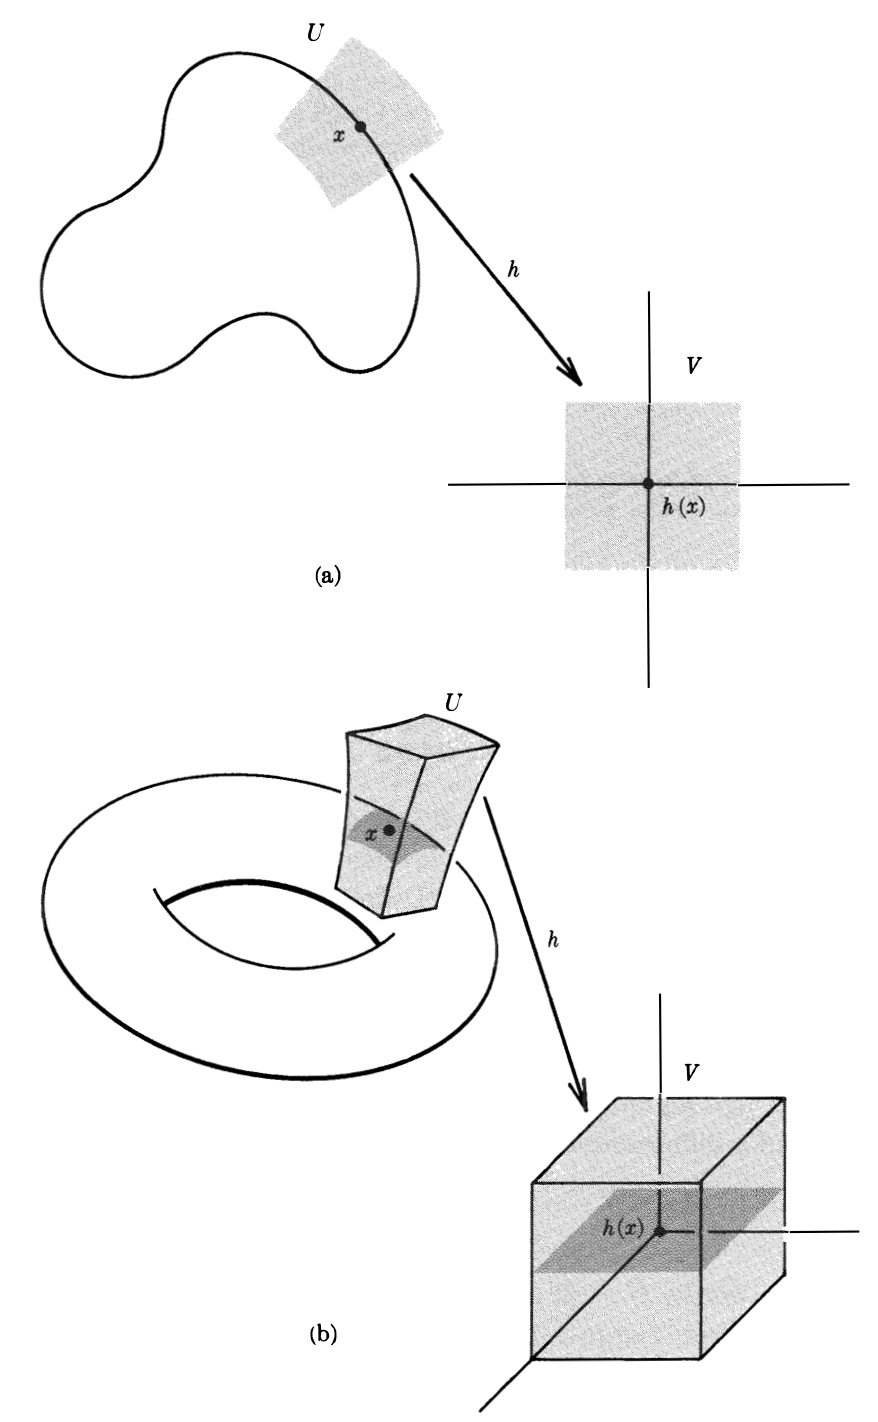
\includegraphics[scale=0.7]{ra_manifold_ex}
\caption{Figure 5.1 in \citet{spivak1971calculus}. (a) A one-dimensional manifold in \(\mathbb{R}^2\). (b) A two-dimensional manifold in \(\mathbb{R}^3\).}
\label{ra_manifold_ex_fig}
\end{center}
\end{figure}

\begin{definition}[\textbf{Topological manifold; definition from \citet{lee2012introduction}, p. 17 of pdf, p. 2 of book}]\label{ra.lee.def.topological manifold}

Suppose \(M\) is a topological space (see Definition \ref{ra.def.topological.space}). We say that \(M\) is a \textbf{topological manifold of dimension \(n\)} or a \textbf{topological \(n\)-manifold} if it has the following properties:

\begin{enumerate}

\item \(M\) is a \textbf{Hausdorff space}: for every pair of distinct points \(p, q \in M\), there are disjoint open subsets \(U, V \subseteq M\) such that \(p \in U\) and \(q \in V\). (This is automatically satisfied for any metric space.)

\item \(M\) is \textbf{second-countable}: there exists a countable basis for the topology of \(M\).

\item \(M\) is \textbf{locally Euclidean of dimension \(n\)}: each point of \(M\) has a neighborhood that is homeomorphic to an open subset of \(\mathbb{R}^n\).

\end{enumerate}

The third property means, more specifically, that for each \(p \in M\) we can find

\begin{itemize}

\item an open subset \(U \subseteq M\) containing \(p\),

\item an open subset \(\hat{U} \subseteq \mathbb{R}^n\), and

\item a homeomorphism \(\phi: U \to \hat{U}\).

\end{itemize}


\end{definition}

\begin{example}


See Figure \ref{ra_manifold_ex_fig} for some examples of manifolds. There are two extreme cases of this definition. \(\mathbb{R}^n\) itself is a topological \(n\)-manifold: it is Hausdorff because it is a metric space, and it is second-countable because the set of open balls with rational centers and rational radii is a countable basis for its topology.


 and an open subset of \(\mathbb{R}^n\) is an \(n\)-dimensional manifold.

Also,  a point in \(\mathbb{R}^n\) is a 0-dimensional manifold,

\end{example}

One common example of an \(n\)-dimensional manifold is the \(n\)-sphere \(S^n\), defined as \(\{x \in \mathbb{R}^{n+1}: |x| = 1\}\). The fact that \(S^n\) is an \(n\)-dimensional manifold can be verified by definition, or more easily by the following result.

\begin{theorem}[\textbf{Theorem 5-1 in \citet{spivak1971calculus}, p. 124 of pdf, p. 111 of book}]\label{ra.spivak.thm.5-1}

Let \(A \subset \mathbb{R}^n\) be open and let \(g: A \to \mathbb{R}^p\) be a differentiable function such that \(g'(x) = (Dg)_{x} \in \mathbb{R}^{p \times n}\) has rank \(p\) whenever \(g(x) = 0\). Then \(g^{-1}(0)\) is an \((n-p)\)-dimensional manifold in \(\mathbb{R}^n\).

\end{theorem}

\begin{proof}

Immediate from Theorem \ref{ra.spivak.thm.2-13}.

\end{proof}


Note that \(S^n = g^{-1}(0)\), where \(g: \mathbb{R}^{n+1} \to \mathbb{R}\) is defined by \(g(x) = |x|^2 -1\).




\begin{definition}[\textbf{Coordinate system or coordinate chart; definition from  \citet{spivak1971calculus}, p. 124 of pdf, p. 111 of book}]\label{ra.spivak.def.coordinate.chart}

Let \(M \subset \mathbb{R}^n\), let \(x \in M\), and let \(U\) be an open set containing \(x\). Let \(W \subset \mathbb{R}^k\). A \textbf{coordinate system} around \(x\) is a one-to-one differentiable function \(f: W \to \mathbb{R}^n\) such that 

\begin{enumerate}

\item \(f(W) = M \cap U\),

\item \(f'(y)\) has rank \(k\) for each \(y \in W\), and

\item \(f^{-1}: f(W) \to W\) is continuous.

\end{enumerate}

See Figure \ref{ra_spivak_5-2_fig}.

\end{definition}

\begin{definition}[\textbf{Coordinate system or coordinate chart; definition from  \citet{lee2012introduction}, p. 19 of pdf, p. 4 of book}]\label{ra.lee.def.coordinate.chart}

Let \(M\) be a topological \(n\)-manifold (see Definition \ref{ra.lee.def.topological manifold}). A \textbf{coordinate chart} (or just a \textbf{chart}) on \(M\) is a pair \((U, \phi)\), where \(U\) is an open subset of \(M\) and \(\phi: U \to \hat{U}\) is a homeomorphism from \(U\) to an open subset \(\hat{U} = \phi(U) \subseteq \mathbb{R}^n\) (see Figure \ref{ra_lee_chart_fig}). By the definition of a topological manifold, each point \(p \in M\) is contained in the domain of some chart \((U, \phi)\). 

If \(\phi(p)= 0\), we say the chart is \textbf{centered at \(p\)}. If \((U, \phi)\) is any chart whose domain contains \(p\), it is easy to obtain a new chart centered at \(p\) by subtracting the constant vector \(\phi(p)\).
%
\begin{figure}[htbp]
\begin{center}
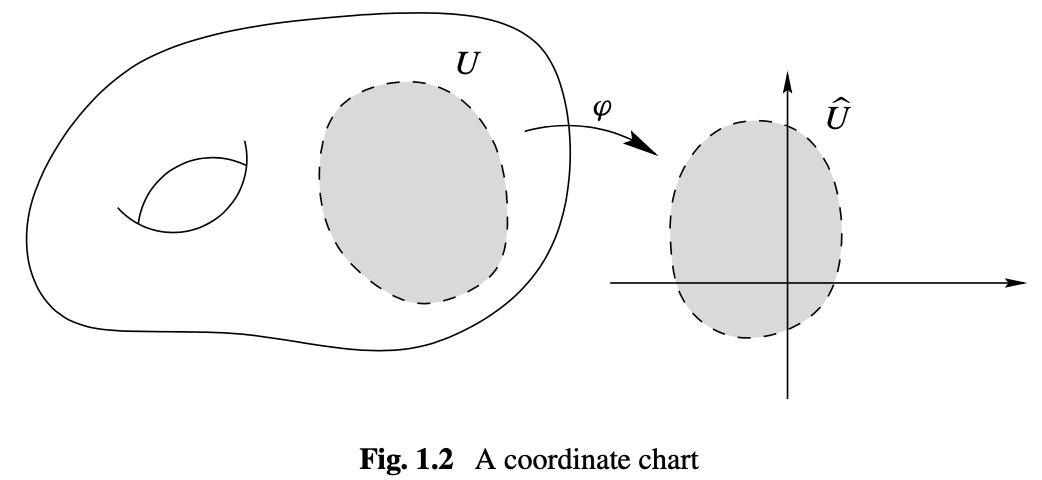
\includegraphics[scale=0.7]{ra_lee_chart}
\caption{Figure 1.2 in \citet{lee2012introduction}; a coordinate chart.}
\label{ra_lee_chart_fig}
\end{center}
\end{figure}

Given a chart \((U, \phi)\), we call the set \(U\) a \textbf{coordinate domain}, or a \textbf{coordinate neighborhood} of each of its points.

% If, in addition, \(\phi(U)\) is an open ball in \(\mathbb{R}^n\).


\end{definition}

The following alternative characterization of manifolds is important.

\begin{theorem}[\textbf{Theorem 5-2 in \citet{spivak1971calculus}, p. 124 of pdf, p. 111 of book}]\label{ra.spivak.thm.5-2}

Let \(M \subset \mathbb{R}^n\), let \(x \in M\), and let \(U\) be an open set containing \(x\). Let \(W \subset \mathbb{R}^k\).  \(M\) is a \(k\)-dimensional manifold if and only if for each \(x \in M\) there is an open set \(U\) containing \(x\) and an open set \(W \subset \mathbb{R}^k\) with a coordinate chart \(f: W \to \mathbb{R}^n\).

\end{theorem}



\begin{figure}[htbp]
\begin{center}
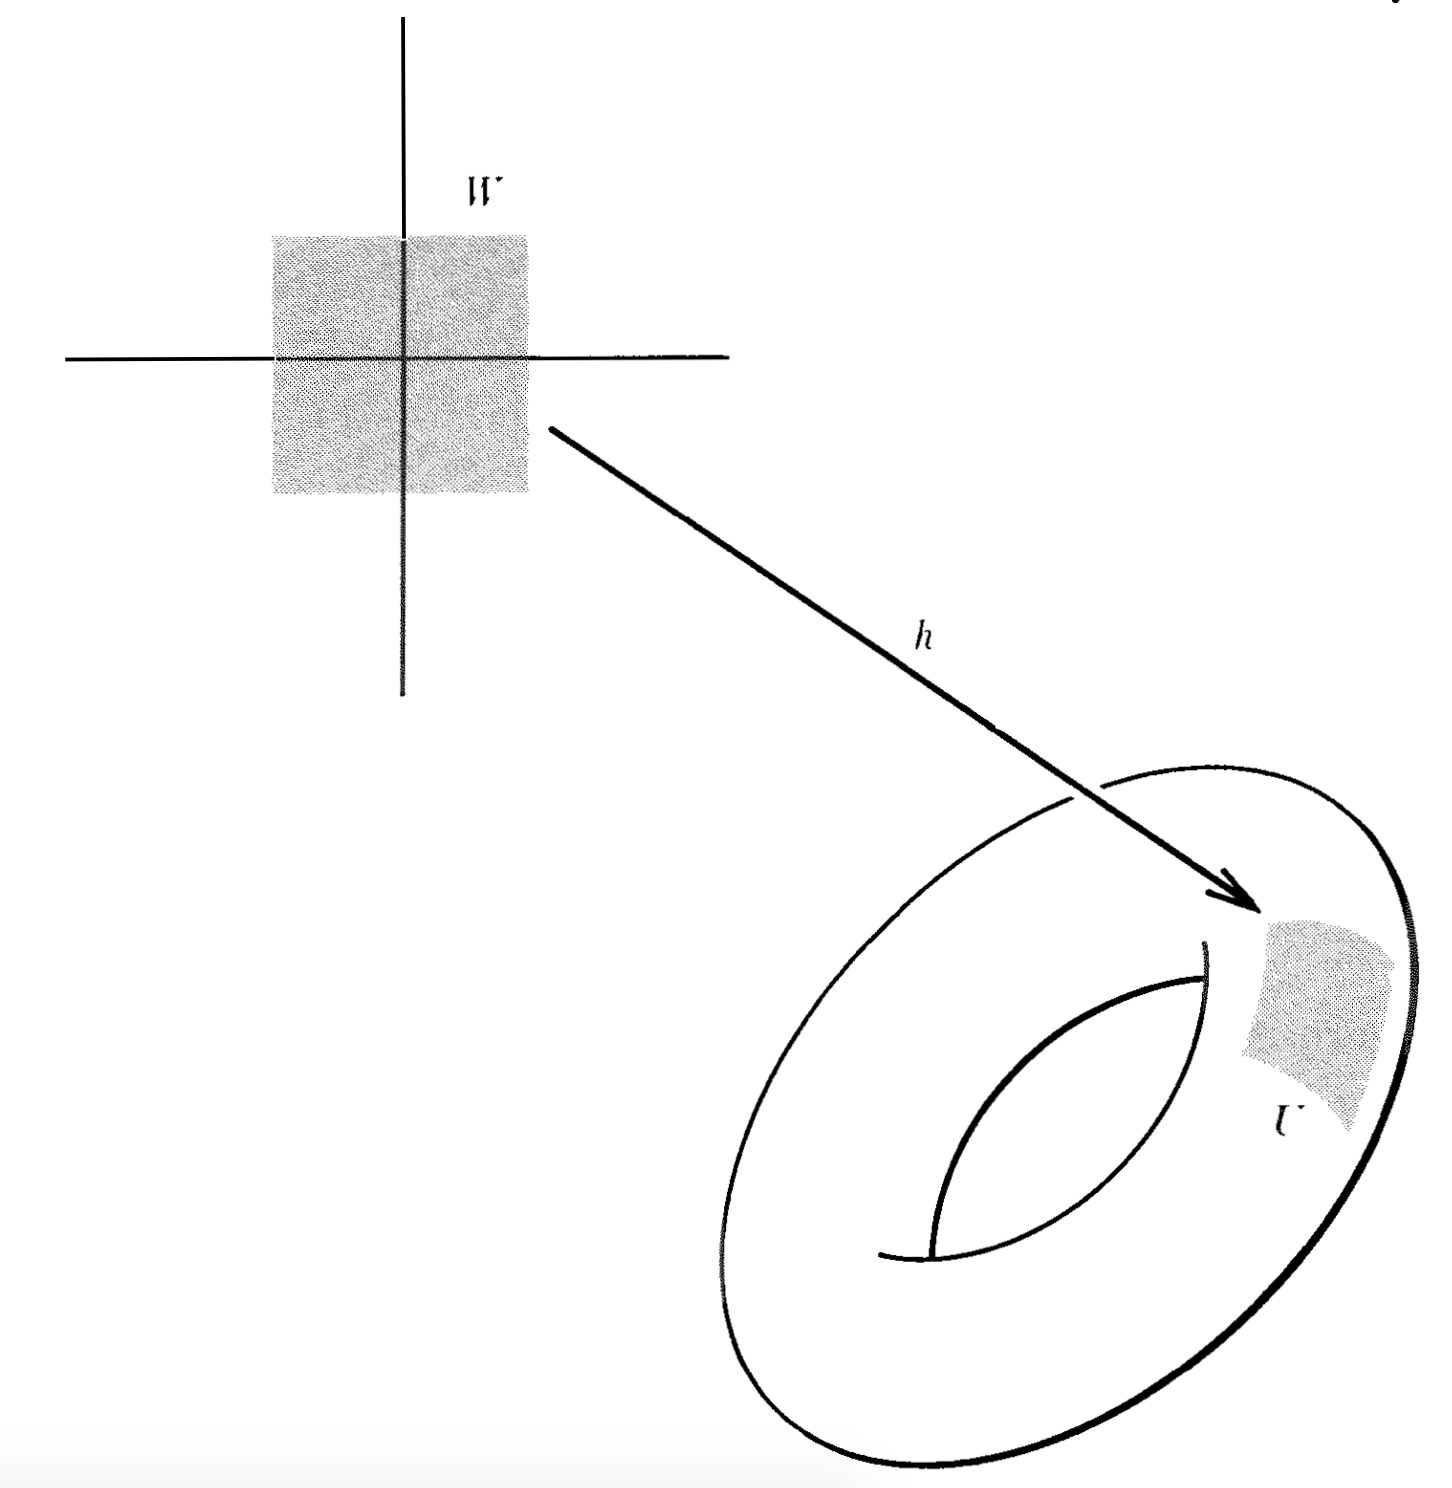
\includegraphics[scale=0.5]{ra_spivak_5-2}
\caption{Figure 5-2 in \citet{spivak1971calculus}, for Theorem \ref{ra.spivak.thm.5-2}.}
\label{ra_spivak_5-2_fig}
\end{center}
\end{figure}


\subsection{Differentiability of functions from \(\mathbb{R}^n \to \mathbb{R}^m\) (Section 5.2 of \citet{pugh2015real})}\label{ra.lin.alg.5.2.pugh}

(See also Section \ref{calc.mat.diff} for more on this material.) 

\begin{definition}[\textbf{Tangent space; from Section 4.2 of \citet{spivak1971calculus}, p. 86 of book, p. 99 of pdf}]\label{ra.def.tangent.space.spivak}

Let \(p \in \mathbb{R}^n\). The set of all pairs \((p,v)\) for \(v \in \mathbb{R}^n\) is denoted \(\mathbb{R}^n_p\) and called the \textbf{tangent space} of \(\mathbb{R}^n\) at \(p\). This set is made into a vector space by defining 

\[
(p,v) + (p,w) = (p, v+ w), \qquad a \cdot (p , v) = (p, av)
\]

for \(v, w \in \mathbb{R}^n\) and \(a \in \mathbb{R}\). In 425b, we use the notation \((T\mathbb{R}^n)_p\).

\end{definition}


\begin{definition}[\textbf{Tangent space; from Section 3.1 of \citet{lee2012introduction}, p. 66 of pdf, p. 51 of book}]\label{ra.def.tangent.space.lee}

Given a point \(a \in \mathbb{R}^n\), define the \textbf{geometric tangent space to \(\mathbb{R}^n\) at \(a\)}, denoted by \(\mathbb{R}^n_a\), to be the set \(\{a\} \times \mathbb{R}^n = \{(a,v): v \in \mathbb{R}^n\}\). A \textbf{geometric tangent vector} in \(\mathbb{R}^n\) is an element of \(\mathbb{R}^n_a\) for some \(a \in \mathbb{R}^n\). 

As a matter of notation, we abbreviate \((a,v)\) as \(v_a\) or sometimes \(v|_a\). n 425b, we use the notation \((T\mathbb{R}^n)_a\).

We think of the vector \(v_a\) as the vector \(v\) with its initial point at \(a\). The set \(\mathbb{R}^n_a\) is a real vector space under the natural operations \(v_a + w_a = (v+w)_a\) and \(c(v_a) = (cv)_a\). The vectors \(e_i |_a, i \in [n]\), are a basis for \(\mathbb{R}_a^n\). 

\end{definition}

Any operations which is possible in a vector space may be performed in each \(\mathbb{R}^n_p\). If a selection of a vector is made in each \(\mathbb{R}^n_p\), we obtain a \textbf{vector field}.

\begin{definition}[\textbf{Vector field; Section 4.2 of \citet{spivak1971calculus}, p. 100 of pdf, p. 87 of book}]\label{ra.def.vector.field}

A \textbf{vector field} is a function \(F\) such that \(F(p) \in \mathbb{R}^n_p\) for each \(p \in \mathbb{R}^n\). For each \(p\) there are numbers \(F^1(p), \ldots, F^n(p)\) such that 

\[
F(p) = F^1(p)\cdot (e_1)_p + \ldots + F^n(p) \cdot (e_n)_p.
\]

We thus obtain \(n\) \textbf{component functions} \(F^i: \mathbb{R}^n \to \mathbb{R}\). The vector field is called continuous, differentiable, etc. if the functions \(F^i\) are. Similar definitions can be made for a vector field defined only on an open subset of \(\mathbb{R}^n\). Operations on vectors yield operations on vector fields when applied at each point separately. For example, if \(F\) and \(G\) are vector fields and \(f\) is a function, we define 

\begin{align*}
(F+G)(p) & = F(p) + G(p), 
\\ \langle F, G \rangle (p) & = \langle F(p), G(p) \rangle,
\\ (f \cdot F)(p) & = f(p) F(p).
\end{align*}

If \(F_1, \ldots, F_{n-1}\) are vector fields on \(\mathbb{R}^n\), then we can similarly define 

\[
(F_1 \times \ldots \times F_{n-1})(p) = F_1(p) \times \ldots \times F_{n-1}(p).
\]

\end{definition}

Matrix for \((DF)_p\) in standard bases for \(\mathbb{R}^n\), \(\mathbb{R}^m\) (\textbf{Jacobian}):

\[
\begin{bmatrix}
\pderiv{F_1}{x_1}(p) & \cdots & \pderiv{F_1}{x_n}(p) \\
\vdots & \ddots & \vdots \\
\pderiv{F_m}{x_1}(p) & \cdots & \pderiv{F_m}{x_n}(p) \end{bmatrix}
\]

We can use this as the definition and we'd be fine for \(C^1\) functions (note: haven't yet defined \(C\) classes for multivariate functions). Important to know about another approach based on an idea of linear approximations.

\begin{definition}[\textbf{Total derivative; Section 5.2 of \citet{pugh2015real}, p. 282 (p. 292 of pdf)}]

Let \(f: U \to \mathbb{R}^m\) be given where \(U\) is an open subset of \(\mathbb{R}^n\). The function \(F\) is \textbf{differentiable} at \(p \in U\) with \textbf{(total) derivative} (or \textbf{Frechet derivative}] \((DF)_p = T\) if \(T \mathbb{R}^n \to \mathbb{R}^m\) is a linear transformation and

\[
\lim_{\lVert v \rVert \to 0} \frac{F(p+ v) - F(p) - T(v)}{ \lVert v \rVert} =0;
\]

that is, (book definition)

\[
R(v) := f(p + v) - f(p) - T(v)   \qquad \implies \qquad \lim_{\lVert v \rVert \to 0} \frac{R(v)}{ \lVert v \rVert} = 0.
\]

\end{definition}

\begin{proposition}[\textbf{Similar to Theorem 5.5 in \citet{pugh2015real}}]

Let \(U \subset \mathbb{R}^n\) be open. Let \(F: U \to \mathbb{R}^m\) be a function and let \(p \in U\). Let \(F = \begin{bmatrix} F_1 \\ \vdots \\ F_m \end{bmatrix}\) , \(F_i : U \to \mathbb{R}\). Then

\begin{enumerate}

\item \(F\) is differentiable at \(p\) with derivative \(T(v) = Av\) (\(A \in \operatorname{Mat}_{m \times n} (\mathbb{R})\)), if and only if 

\item Each \(f_i\) is differentiable at \(p\) with derivative \(T_i(v) = \begin{bmatrix} a_{i1} & \cdots & a_{in} \end{bmatrix} \begin{bmatrix} v_1 \\ \vdots \\ v_n \end{bmatrix}\).

\end{enumerate}



\end{proposition}

\begin{proof}

(1) is true if and only if \(\lim_{\lVert v \rVert \to 0} \frac{F(p+ v) - F(p) - T(v)}{ \lVert v \rVert} =0\), which is true if and only if each coordinate of \( \frac{F(p+ v) - F(p) - T(v)}{ \lVert v \rVert} \to 0\) as \(v \to 0\), which is true if and only if (2) is true.

\end{proof}

Next we will talk about uniqueness. We want to show that \(T = (DF)_p\) is unique if it exists. This is easy if we use the chain rule (the book is quicker and more direct but a bit redundant).

\begin{proposition}[\textbf{Differentiability implies continuity; Theorem 5.6 in \citet{pugh2015real}}]\label{ra.diff.imp.cont.mult}

Let \(U \subset \mathbb{R}^n\) be open. Let \(p \in U\), \(F: U \to \mathbb{R}^m\). If \(F\) is differentiable at \(p\) with derivative \(T\), then \(F\) is continuous at \(p\).

\end{proposition}

\begin{proof}

We have \(F(p+v) = F(p) + T(v) + R_F(v)\), where \(\lim_{v \to 0} \frac{ \lVert R_F(v) \rVert}{\lVert v \rVert} = 0\). This implies \(\lim_{v \to 0} \lVert R_F(v) \rVert = 0\) (note: \(\lVert R_F(v) \rVert \leq \frac{ \lVert R_f(v) \rVert}{\lVert v \rVert}\) for \(\lVert v \rVert \leq 1\)). Therefore \(\lim_{ v\to 0} F(p+v) = F(p) + 0 + 0\); that is, for every \(\epsilon >0\) there exists \(\delta > 0\) such that \(\lVert v \rVert_2 < \delta \implies \lVert F(p + v) - F(p) \rVert_2 < \epsilon\), so \(F\) is continuous at \(p\).

\end{proof}

\begin{theorem}[\textbf{Chain rule; Theorem 5.9(c) in \citet{pugh2015real}}]\label{ra.thm.multi.chain.rule}

Let \(U \subset \mathbb{R}^n\) be open. Let \(V \subset \mathbb{R}^m\) be open. Let \(F: U \to V\) and let \(G: V \to \mathbb{R}^k\) be functions such that (1) \(F\) is differentiable at \(p\) (with derivative \(A\)) and (2) \(G\) is differentiable at \(F(p) = q \in V\) (with derivative \(B\)). Then \(G \circ F\) is differentiable at \(p\) with derivative \(B \circ A\). 

\end{theorem}

Note that if the derivative is unique, then \((D(G \circ F))_p = (DG)_{f(p)} \circ (DF)_p\) (composing then linearly approximating is the same as linearly approximating then composing). 

\begin{proof}

Let \(R_F = R_{F, p,A}\), a function of \(v  \in \mathbb{R}^n\). \(R_F(v) = F(p + v) - F(p) - Av\), so 

\begin{equation}\label{ra.chain.rule.mult.1}
F(p + v) = F(p) + Av + R_F(v).
\end{equation}

 Let \(R_G = R_{G, q, B}\), a function of \(w \in \mathbb{R}^m\). \(R_G(w) = G(q + w) - G(q) - Bw\), so 
 
 \begin{equation}\label{ra.chain.rule.mult.2}
 G(q + w) = G(q) + Bw + R_G(w).
 \end{equation}
 
Let \(R_{G \circ F} = R_{G \circ F, p, BA}\). We want to show that \(\lim_{v \to 0} \frac{R_{G \circ F}}{\lVert v \rVert} = 0\).

We have

\begin{align*}
R_{G \circ F} (v) & = (G \circ F)(p + v) - (G \circ F)(p) - BAv
\\ & = G(F(p+v)) - G(\underbrace{F(p)}_{=q}) - BAv
\\ \text{(by (\ref{ra.chain.rule.mult.1}))} \qquad & = G(F(p) + Av + R_F(v)) - G(q) - BAv
\\  \text{(by (\ref{ra.chain.rule.mult.2}) and \(F(p) = q\))} \qquad  & = G(q) + B(Av + R_F(v)) + R_G(Av + R_F(v)) - G(q) - BAv
\\ & = BR_F(v) + R_G(Av + R_F(v)).
\end{align*}

%(Note that \(F(p+v)\) is close to \(q = F(p)\). In the next step we used an approximation for \(G\), including the error term. We also used \(G(q+w) = G(q) + Bw + R_G(w)\).) 

Thus,

\begin{equation}\label{ra.chain.rule.mult.proof}
\frac{ \lVert R_{G \circ F}(v) \rVert}{\lVert v \rVert}  \leq \frac{\lVert B R_F(v) \rVert}{\lVert v \rVert} + \frac{ \lVert R_G(Av + R_F(v)) \rVert}{\lVert v \rVert}.
\end{equation}

We want to show both terms on the right in (\ref{ra.chain.rule.mult.proof}) go to 0 as \(v \to 0\). First,

\[
\frac{\lVert B R_F(v) \rVert}{\lVert v \rVert}  \leq \lVert B \rVert_{\text{op}} \frac{ \lVert R_F(v) \rVert}{\lVert v \rVert} \to 0
\]

as \(v \to 0\) by differentiability of \(F\) (since \(\lVert B \rVert_{\text{op}} < \infty\)). Next, for \(v\) with \(Av+ R_F(v) = 0\), we have

\[
R_G(Av + R_F(v)) = R_G(0) = 0
\]

since \(R_G(w) = G(q + w) - G(q) - Bw \implies R_G(0) = G(q) - G(q) - 0 = 0\). Thus the second term in (\ref{ra.chain.rule.mult.proof}) is 0 if \(v \neq 0\) and \(Av + R_V(v) = 0\). For \(x\) with \(Av + R_F(v) \neq 0\), we have

\[
 \frac{ \lVert R_G(Av + R_F(v)) \rVert}{\lVert v \rVert} =  \frac{ \lVert R_G(Av + R_F(v)) \rVert}{ \lVert Av + R_F(v) \rVert}  \frac{ \lVert Av + R_F(v) \rVert}{\lVert v \rVert}
\]

As \(v \to 0\) we have \(Av + R_F(v) \ \to 0\), since matrix multiplication by \(A\) is continuous and \(R_F(v) = F(p+v) - F(p) - Av\) is continuous at \(v=0\) (since differentiability of \(F\) at \(p\) implies continuity of \(F\) at \(p\) by Proposition \ref{ra.diff.imp.cont.mult}). Since \(\lim_{v \to 0} (Av + R_F(v) ) = 0\) and \(\lim_{w \to 0} \frac{ \lVert R_G(w) \rVert}{\lVert w \rVert} = 0\), we have 

\[
\lim_{v \to 0}  \frac{ \lVert R_G(Av + R_F(v)) \rVert}{ \lVert Av + R_F(v) \rVert} = 0.
\]

From here it is enough to show that \(\lim_{v \to 0}  \frac{ \lVert Av + R_F(v) \rVert}{\lVert v \rVert} \) is bounded. Observe that

\[
 \frac{ \lVert Av + R_F(v) \rVert}{\lVert v \rVert} \leq \frac{ \lVert Av \rVert}{\lVert v \rVert} + \frac{ \lVert R_F(v) \rVert}{\lVert v \rVert} \leq \lVert A \rVert_{\text{op}} + 0.
\]

\end{proof}

An important geometric interpretation that gives us the uniqueness of derivatives: \((DF)p\) is determined by how it acts on velocity vectors of curves (see notes).

\begin{corollary}

Let \(U \subset \mathbb{R}^n\) be open. Let \(p \in U\), \(F: U \to \mathbb{R}^m\). Let \(0 \in (a,b)\) and let \(\gamma: (a,b) \to U\) be a differentiable function (curve) with \(\gamma(t_0) = p\). Then \((DF)_p(\gamma'(t_0)) = (F \circ \gamma)'(t_0)\).

\end{corollary}

\begin{proof}

By the chain rule (Theorem \ref{ra.thm.multi.chain.rule}), \(F \circ \gamma\) is differentiable at \(t_0\) with \((D(F \circ \gamma))_{t_0} = (DF)_{\gamma(t_0)} (D \gamma)_{t_0} =  (DF)_{p} (D \gamma)_{t_0}\). Viewed as a \(m \times 1\) matrix, we showed last time that \((D(F \circ \gamma))_{t_0} = (F \circ \gamma)'(t_0)\). Viewed as an \(n \times 1\) matrix, we showed that \((D \gamma)_{t_0} = \gamma'(t_0)\).

\end{proof}
 
 \begin{corollary}
 
 If \(F\) is differentiable at \(\gamma(t_0)) =p\) with derivative \(T = (DF)_p\), then 
 
 \[
 T(v) = \lim_{t \to 0} \frac{F(p+tv) - F(p)}{t}.
 \]
 
  (since the right side is independent of \(T\), this shows \(T\) is unique.)
 
 \end{corollary}
 
 \begin{proof}
 
 Let \(\gamma(t) = p + tv\); then the right hand side is \((F \circ \gamma)'(t_0)\) (using \(\gamma(t_0) = p\)).
 
 \end{proof}
 
 If \(\lim_{t \to 0} \frac{f(p+tv) - F(p)}{t}\) exists for all \(v\) (this is \((DF)_p(v)\)) and this quantity is linear in \(v\), is \(F\) (Frechet) differentiable at \(p\)? No. For example, \(F: \mathbb{R}^2 \to \mathbb{R}\), 
 
 \[
 F(x,y) = \begin{cases} 
 \frac{x^3 y}{x^4 + y^2}, & (c, y) \neq (0,0), \\
 (0, 0), & (x,y) = (0,0).
 \end{cases}
 \]
 
 Exercise (\citet{pugh2015real} ex. 18 and 19, ch 5; more discussion on why to prefer Frechet): directional derivative exists and equals 0 for all \(v\) but \(F\) is not differentiable at \((0,0)\). 
 
 \begin{proposition}[\textbf{Theorem 5.9(a) and 5.9(b) in \citet{pugh2015real}}]\label{ra.sum.scal.diff.mult.diff}
 
 Let \(U \subset \mathbb{R}^n\) be open. Let \(p \in U\), \(F, G : U \to \mathbb{R}^m\).
 
 \begin{enumerate}[(a)]
 
 \item If \(F\) and \(G\) are differentiable at \(p\) then \(F+G\) is differentiable at \(p\) with \(D(F+G)p = (DF)p + (DG)p\).
 
 \item If \(c \in \mathbb{R}\) then \(cF\) is differentiable at \(p\) with \(D(cF)_p = c (DF)_p\).
 
 \item Any constant function \(F: U \to \mathbb{R}^m\) is differentiable with derivative 0 everywhere.
 
 \item If \(F:U \to \mathbb{R}^m\) is affine linear (\(F(x) = Ax + y_0\) for some \(A \in \mathbb{R}^{m \times n}\), \(y_0 \in \mathbb{R}^m\)) then \(F\) is differentiable at all points of \(U\) with derivative \(A\).
 
 \end{enumerate}
 
 \end{proposition}
 
 \begin{proof}
 
  \begin{enumerate}[(a)]
 
 \item 
 
 \begin{align*}
&  \frac{ \lVert (F+G)(p+v) - (F+G)(p) - ( (DF)_p + (DG)_p)(v) \rVert}{\lVert v \rVert}
\\ \leq &  \frac{ \lVert F(p+v) - F(p) - (DF)_p (v) \rVert}{\lVert v \rVert} +  \frac{ \lVert G (p+v) - G(p) - (DG)_p(v) \rVert}{\lVert v \rVert}.
 \end{align*}
 
 Each of these terms goes to 0 as \(v \to 0\) by differentiability of \(F\) and \(G\).
 
 \item

 
 \[
  \frac{ \lVert (cF)(p+v) - (cF)(p) -  D[cF])_p (v) \rVert}{\lVert v \rVert}  \leq c  \frac{ \lVert F(p+v) - F(p) - (DF)_p (v) \rVert}{\lVert v \rVert} 
\]

which goes to 0 as \(v \to 0\) by differentiability of \(F\).

 \item 
 
 \item If \(F(x) = Ax + y_0\) then 
 
 \begin{align*}
 \frac{F(p+v) - F(p) - Av}{\lVert v \rVert} = \frac{ A(p+v) - A(p) - A(v) }{\lVert v \rVert} = \frac{0}{\lVert v \rVert} \to 0 
 \end{align*}
 
 as \(v \to 0\).
 
 \end{enumerate}
 
 \end{proof}
 
 \begin{definition}
 
 Let \(U \subset \mathbb{R}^n\) be open. Let \(p \in U\) and let \(F: U \to \mathbb{R}^m\). Let \(1 \leq i \leq n\). The \textbf{\(i^{\text{th}}\) partial derivative} of \(F\) at \(p\), \(\pderiv{F}{x_i}(p)\), is defined to be
 
 \[
 \pderiv{F}{x_i}(p) := \lim_{t \to 0} \frac{F(p +  t e_i) - F(p)}{t}
 \]
 
 (if it exists) where \(e_i\) is the \(i^{\text{th}}\) standard basis vector for \(\mathbb{R}^n\) (the directional derivative of \(F\) in the direction \(e_i\)). If \(F\) is differentiable, it also equals \((DF)_p(e_i) = (F \circ \gamma)'(0)\) where \(\gamma(t) = p + t e_i\). 
 
 \end{definition}
 
 \begin{remark}
 
 If \(F: U \to \mathbb{R}^m\) and \(\pderiv{F}{x_i}(p)\) exists for all \(p \in U\), then \(\pderiv{F}{x_i}: U \to \mathbb{R}^m\) (just the \(F\)). This implies we can (try to) take successive derivatives, e.g., we can do
 
 \[
 \pderiv{^2 F}{x_j \partial x_i} := \pderiv{}{x_j} \left( \pderiv{F}{x_i} \right) ,
 \]
 
 etc., and keep getting functions from \(U\) to \(\mathbb{R}^m\) as long as the partial derivatives keep existing.
 
 \end{remark}
 
 \begin{definition}
 
 Let \(F: U \to \mathbb{R}^m\) is of \textbf{class \(C^k\)} (we can also say \(F\) is a \textbf{\(C^k\) function}) if all partial derivatives of \(F\) of orders \(\leq k\) exist and are continuous in \(U\). (We use this notation with \(k = \infty\) if this is true for all orders, not ``infinite orders.") We call \(C^\infty\) functions \textbf{smooth}.
 
 \end{definition}
 
 \begin{theorem}\label{ra.thm.jacobian}
 
 If \(F: U \to \mathbb{R}^m\) is of class \(C^1\), then \(F\) is differentiable at all \(p \in U\) and \( (DF)_p : \mathbb{R}^n \to \mathbb{R}^m\) has standard basis matrix
 
 \begin{equation}\label{ra.thm.jacobian.mat}
 \begin{bmatrix}
 \pderiv{F_1}{x_1}(p) & \cdots & \pderiv{F_1}{x_n}(p) \\
 \vdots & \ddots & \vdots \\
 \pderiv{F_m}{x_1}(p) & \cdots & \pderiv{F_m}{x_n}(p)
 \end{bmatrix}
 \end{equation}
 

 
 \end{theorem}
 
 \begin{remark}
 
  Note that the columns are \(\pderiv{F}{x_i}(p)\) for \(i \in [n]\). This makes sense: if \(\lim_{t \to 0} \frac{F(p+v) - F(p)}{t}\) is linear in \(v\), then the \(i\)th column of its standard basis matrix should be obtained by plugging \(v=e_i\) into \(\lim_{t \to 0} \frac{F(p+v) - F(p)}{t}\).
  
  \end{remark}
  
  \begin{proof}
  
Let \(J\) be the matrix (\ref{ra.thm.jacobian.mat}). Let \(T(v) = Jv\) (\(T: \mathbb{R}^n \to \mathbb{R}^m\) linear). Let \(R(v) = F(p+v) - F(p) - Jv\). For \(i \in [m]\), let \(R_i(v) \) be the \(i^\text{th}\) coordinate of \(R(v)\). Then

\[
R_i(v) = F_i(p+v) - F_i(p) - \begin{bmatrix} \pderiv{F_i}{x_1}(p) & \cdots &  \pderiv{F_i}{x_n}(p) \end{bmatrix} v.
\]

It suffices to show \(\frac{R_i(v)}{\lVert v \rVert} \to 0\) as \(v \to 0\) for \(i \in [m]\). (Then each point of \(\frac{R(v)}{\lVert v \rVert} \to 0\), so \(\frac{R(v)}{\lVert v \rVert} \to 0\) as \(v \to 0\).) Given \(\epsilon > 0\), choose \(\delta > 0\) such that if \(\lVert v \rVert < \delta\) then (a) \(p + v \in U\) and \(b\) \( \left| \pderiv{F_i}{x_j} (p + d) - \pderiv{F_i}{x_j}(p) \right| < \epsilon/n\) for \(j \in [n]\) (\(i\) is fixed). (Recall that using the \(C^1\) assumption, \(\pderiv{F_i}{x_j}\) is continuous at \(p\) for \(j \in [n]\).) 

We claim that if \(\lVert v \rVert < \delta\) then \(\frac{ | R_i(v)|}{\lVert v \rVert} < \epsilon\), proving the theorem. To see this, let \(v\) be fixed with \(\lVert v \rVert < \delta\) (\(v = \begin{bmatrix} v_1 \\ \vdots \\ v_n \end{bmatrix}\)). We have

\[
R_i(v) = F_i(p+v) - F_i(p) - V_1 \pderiv{F_i}{x_1}(p) - \ldots - v_n \pderiv{F_i}{x_n}(p).
\]
  
We can write 

\begin{align*}
F_i(p+v) - F_i(p)  = & F_i(p + V_1 e_1 + \ldots + v_n e_n) - F_i(p)
\\  = &  F_i(p + v_1 e_1 + \ldots + v_n e_n) - F_i(p + V_1 e_1 + \ldots + v_{n-1} e_{n-1}) 
\\ & + F_i(p + v_1 e_1 + \ldots + v_{n-1} e_{n-1}) - F_i(p + v_1e_1 + \ldots + v_{n-2} e_{n-2}) 
\\ & + F_i(p + v_1 e_1+ \ldots + v_{n-2} e_{n-2}) - \ldots + F_i(p + v_1 e_1) - F_i(p)
\end{align*}  

It suffices to show 

\[
\frac{ \left| F_i(p + v_1 e_1 + \ldots + v_j e_j) - F_i(p + V_1 e_1 + \ldots + v_{j-1} e_{j-1}) \right|}{\lVert v \rVert} < \epsilon/n
\]

for \(2 \leq j \leq n\). We will use the one-variable MVT. First: if \(v_j = 0\), then \(p_j = p_{j-1}\) and the whole thing is 0. Assume note. Use a path \(\sigma_j\) starting at \(p_{j-1}\) and ending at \(p_j\) (these paths \(\sigma\) form the ``staircase path" from \(p\) to \(p+v\) shown in Figure 108, p. 285 (p. 295 of pdf) in \citet{pugh2015real}). Indeed: let \(\sigma_j(t) := p_{j-1} + t v_j e_j\) for \(t \in[0,1]\). \(F_i \circ \sigma_j(t) = F_i(p_{j-1} + t v_j e_j)\); derivative quotient is 

\begin{align*}
\lim_{t' \to t} \frac{F_i(p_{j-1} + t' v_j e_j) - F_i(p_{j-1} + t v_j e_j) }{t' - t} & = v_j \lim_{t' \to t} \frac{F_i(p_{j-1} + t' v_j e_j) - F_i(p_{j-1} + t v_j e_j) }{v_j t' - v_j t} 
\\ & =  \lim_{t' \to t} \frac{F_i(p_{j-1} + t' v_j e_j) - F_i(p_{j-1} + t v_j e_j) }{ t' - t} 
\\ & = \pderiv{F_i}{x_j}(p_{j-1} + t e_j)
\end{align*} 

since \(t' \to t \iff v_j t' \to v_jt\). \(\pderiv{F_i}{x_j}(p_{j-1} + t e_j)\) exists for all \(t \in [0,1]\), so we get \(F_i \circ \sigma_j\) is a differentiable function from \([0,1] \to \mathbb{R}\) with derivative \(v_j \pderiv{F_i}{x_j} (p_{j-1} + t e_j)\) at the point \(t \in [0,1]\). Let \(p_{ij} := p_{j-1} + t e_j\). By the Mean Value Theorem, there exists \(t \in [0,1]\) with \(F_i(\sigma_j(1)) - F_i(\sigma_j(0)) = v_j \pderiv{F_i}{x_j} (p_{ij}) \) (\(\sigma_j(1) = p_j\), \(\sigma_j(0) = p_{j-1}\)). Thus,

\begin{align*}
\frac{ \left| F_i(p_j) - F_i(p_{j-1}) - \pderiv{F_i}{x_j}(p) v_j \right|}{\lVert v \rVert} & = \frac{1}{\lVert v \rVert} \left| v_j \left( \pderiv{F_i}{x_j}(p_{ij}) - \pderiv{F_i}{x_j}(p) \right) \right|
\\ & \leq \left| \pderiv{F_i}{x_j}(p_{ij}) - \pderiv{F_i}{x_j}(p) \right|
\\   & < \frac{\epsilon}{n}
\end{align*}

where we used \(| v_i|/\lVert v \rVert \leq 1\), and the last step follows since \(\lVert p_{ij} - p \rVert < \delta\) (indeed: \(p_{ij} - p = v_1 e_1 + \ldots + v_{j-1} e_{j-1} + t v_j e_j\) for \(t \in [0,1]\), and \(v = v_1 e_1 + \ldots + v_n e_n\), so \( \lVert p_{ij} - p_j \rVert \leq \lVert v \rVert < \delta\), finishing the proof.
  
  \end{proof}
  
\begin{example}

Define \(F: \mathbb{R}^3 \to \mathbb{R}^3\) by 

\[
F(x,y,z) := \begin{bmatrix} e^z \cos (y) \\ e^{-z} \sin(y) \\ x^2 + y^2 + z^3 \end{bmatrix}. 
\]

Is \(F\) differentiable? Yes, \(F\) is \(C^1\) (even \(C^\infty\)) by inspection of each component. In particular,

\[
(DF)_{(x,y,z)} = \begin{bmatrix}
0 & -e^z \sin(y) & e^z \cos(y) \\
0 & e^{-z} \cos(y) & -e^{-z} \sin(y) \\
2x & 2y & 2z
\end{bmatrix}.
\]

\end{example}

\begin{theorem}[\textbf{Mean Value Theorem for functions from \(\mathbb{R}^n\) to \(\mathbb{R}\)}]

Let \(U \subset \mathbb{R}^n\) be open. Let \(F: U \to \mathbb{R}\) be differentiable. Let \(p, q \in U\) such that \(p + t(q-p) \in U\) for \(t \in [0,1]\). Then there exists \(\theta \in [0,1]\) with \(F(q) -F(p) = (DF)_{p + \theta (q-p)} (q-p)\).

\end{theorem}

\begin{proof}

Apply the one-variable Mean Value Theorem to \(F(p + t(q-p))\), a differentiable function from \([0,1] \to \mathbb{R}\). The derivative at \(\theta\) is \((DF)_{p+\theta(q-p)}(q-p)\). Then

\[
F(\underbrace{p+1 (q-p)}_{q}) - F(\underbrace{p + 0(q-p)}_{p}) = \left((DF)_{p+\theta(q-p)}(q-p \right)(1-0).
\]

\end{proof}

On the other hand, the case of vector-valued functions isn't so simple.

\begin{example}

Consider \(F: \mathbb{R} \to \mathbb{R}^2\) defined by \(F(t) = (\cos t, \sin t)\). Then observe that 

\[
\underbrace{F(2\pi) - F(0)}_0 =? (DF)_t(2\pi -0) \qquad \text{for any } t?
\]

But

\[
\begin{bmatrix} 
- \sin t \\
\cos (t)
\end{bmatrix} \neq 0
\]

for any \(t\).

\end{example}

What do we do in this case?

\begin{theorem}[\textbf{Mean value inequality; Theorem 5.11 in \citet{pugh2015real}, p. 298 of pdf, p. 288 of book}]

Let \(U \subset \mathbb{R}^n\) be open. Let \(F: U \to \mathbb{R}^m\) be differentiable. Let \(p, q \in U\) such that the line segment \(\{p + t(q-p) \mid t \in [0,1]\} \subset U\). Then

\[
\lVert F(q) - F(p) \rVert \leq \left( \sup_{t \in [0,1]} \lVert (DF)_{p + t(q-p)} \rVert_{\text{op}} \right) \lVert q -p \rVert
\]

(Note that this is upper-bounded by 

\[
\left(\sup_{x \in U} \lVert (DF)_x \rVert_{\text{op}} \right) \lVert q - p \rVert,
\]

which is the version shown in \citet{pugh2015real}.)

\end{theorem}

\begin{proof}

If we can show that for some \(M \in \mathbb{R}\) \(\langle F(q) - F(p), u \rangle \leq M \lVert q - p \rVert\) for all unit vectors \(u \in \mathbb{R}^m\), then we're done because we can take \(u  = (F(q) - F(p))/\lVert F(q) - F(p) \rVert\) and get the statement of the theorem. Let \(v := q-p\) and let 

\[
g(t) := \langle F(p+tv), u \rangle = \sum_{i=1}^m u_i F_i(p+tv) 
\]

(if \(u = (u_1, \ldots, u_m)^\top\) and \(F = (F_1, \ldots, F_m)^\top\)). Each \(F_i\) is differentiable, and \(t \mapsto p + tv\) is differentiable, so \(F_i(p + tv)\) is a differentiable function of \(t\). Sums and scalar multiples of differentiable functions are differentiable by Proposition \ref{ra.sum.scal.diff.mult.diff}, so \(g(t)\) is differentiable. In particular,

\[
g'(t) = \sum_{i=1}^m u_m (DF_m)_{p + tv}(v) = \langle (DF)_{p + tv}(v), u \rangle.
\] 

(Note that this equation also results from the Leibniz rule, although we didn't prove the Leibniz rule.) By the one-dimensional Mean Value Theorem for \(g\), there exists \(\theta \in [0,1]\) with 

\[
 g'(\theta)(1-0) = g(1) - g(0) = \langle F(q), u \rangle - \langle F(p), u \rangle = \langle F(q) - F(p), u \rangle
\]

Observe that 

\[
 g'(\theta)(1-0) = \langle (DF)_{p+ \theta v}(v), u \rangle  \leq \text{(by Cauchy-Schwarz) } \lVert (DF)_{p + \theta v}(v) \rVert \underbrace{\lVert u \rVert}_q \leq  \underbrace{\lVert (DF)_{p + \theta v} \rVert_{\text{op}}}_{\leq M} \underbrace{\lVert v \rVert }_{= \lVert q - p \rVert} .
 \]
 
 So we've shown \(\langle F(q) - F(p), u \rangle \leq M \lVert q - p \rVert\) for all unit vectors \(u \in \mathbb{R}^m\), proving the theorem.

\end{proof}

\begin{theorem}[\textbf{\(C^1\) Mean Value Theorem: may do later}]

\end{theorem}

\begin{corollary}

If \(U \subset \mathbb{R}^n\) is open and connected and \(F: U \to \mathbb{R}^m\) is differentiable with \((DF)_x = 0\) for all \(x \in U\), then \(F\) is constant.

\end{corollary}

\begin{proof}

Exercise, use topological fact: any two points in \(U\) can be connected by a differentiable path \(\gamma\) since \(U\) is connected.

\end{proof}

\begin{theorem}[\textbf{Differentiation under the integral sign}]

Let \(f: [a,b] \times (c,d) \to \mathbb{R}\) (or \(\mathbb{R}^m\)) be a continuous function. Assume \(\pderiv{f}{y}(x,y)\) is also continuous. Let \(F(y) = \int_a^b f(x,y) dx\). Then \(F\) is differentaible on \((c,d)\) with \(F'(y) = \int_a^b \pderiv{f}{y} (x,y) dx\); i.e., \(\pderiv{}{y} \int_a^b f(x,y) dx = \int_a^b \pderiv{}{y} f(x,y) dx\). 

\end{theorem}

\begin{remark}

Better theorems exist under Lebesgue theory.

\end{remark}

\begin{proof}

In the book, uses \(C^1\) Mean Value Theorem. We'll skip for now.

\end{proof}

\subsection{Implicit and Inverse Functions Theorems (Section 5.4 of \citet{pugh2015real})}\label{ra.5.4.pugh}

We will start with the Implicit Function Theorem and use it to deduce the Inverse Function Theorem. Here is the basic idea: say we have \(n + m\) variables \(x_1, \ldots, x_n, y_1, \ldots, y_m\), and we impose \(m\) nonlinear constraints: we look at points \((x,y) := (x_1, \ldots, x_n, y_1, \ldots, y_m)\) such that \(F(x,y) = z\) where \(F : \mathbb{R}^{n + m} \to \mathbb{R}^m\) is some function and \(z \in \mathbb{R}^m\). (\(F\) has coordinates \(F_1, \ldots, F_m\); \(F(x,y) = z\) amounts to \(m\) scalar equations. So we have \(m\) constraints \(F_i(x,y) = z_i\), \(i \in [m]\).)

\begin{example}

Let \(n=1, m=1, F(x,y) = x^2 + y^2, z = 1\). Then \((x,y) \in \mathbb{R}^2\) must lie on the unit circle.

Let \((x_0, y_0) \in F^{-1}(z)\) (the level set of \(F\) at level \(z\)). The main question for the Implicit Function Theorem is: locally near \((x_0, y_0)\), can we write \(F^{-1}(z)\) as a graph of \(y\) as a function of \(x\) (or \(x\) as a function of \(y\))?

In this case, if \((x_0, y_0) \neq (\pm 1, 0)\), then we can write the local part of the circle as a graph of \(y\) as a function of \(x\), namely \(y = \pm \sqrt{1-x^2}\) (pick which one depending on sign of \(y_0\)). However if \((x_0, y_0) \in \{(1,0), (-1,0)\}\), we can't express \(y\) locally as a function of \(x\), although we can express \(x\) as a function of \(y\) (although not near \((0, \pm1)\)). So we have four open subsets of the circle where \(F^{-1}(z)\) can be written locally as a graph.

\end{example}

\begin{definition}\label{ra.def.graph}

Let \(f: A \to B\) be a function. The \textbf{graph} of \(f\) is the set \(S\) of all pairs \((a,b) \in A \times B\) such that \(b = f(a)\).

\end{definition}

\begin{theorem}[\textbf{Implicit Function Theorem (Dini 1876; Theorem 5.22 in \citet{pugh2015real})}]\label{ra.imp.fxn.thm}

Let \(U \subset \mathbb{R}^{m+n}\) be open. Let \(F: U \to \mathbb{R}^m\) be a class of \(C^r\) functions for \(r \geq 1\). Let \((x_0, y_0) \in U\) (\(x_0 \in \mathbb{R}^n, y_0 \in \mathbb{R}^m\)), let \(z_0 \in \mathbb{R}^m\) with \(F(x_0, y_0) = z_0\), and \((DF)_{(x_0, y_0)} \in \mathbb{R}^{m \times (n +m)}\) have the form \(\begin{bmatrix} A & B \end{bmatrix}\) with \(A \in \mathbb{R}^{m \times n}\) and \(B \in \mathbb{R}^{m \times m}\) with \(B\) invertible\footnote{Note that any full rank matrix of size \(m \times (m + n)\) can have this form, possibly after permuting columns.}. Then there exists \(r, \tau > 0\) such that \(B_\tau(x_0) \times B_r(y_0) \subset U\) such that there exists a unique function \(g: B_\tau(x_0) \to B_r(y_0)\) with \(F^{-1}(z_0) \cap ( B_\tau(x_0) \times B_r(y_0)) = \operatorname{graph}(g) = \{(x, g(x)): x \in B_\tau(x_0)\}\) (see Definition \ref{ra.def.graph}). This function \(g\) is of class \(C^r\). 

(For notational ease, assume without loss of generality that \((x_0, y_0)\) is the origin in \(\mathbb{R}^{n + m}\) and \(z_0 = 0 \in \mathbb{R}^m\).)

\end{theorem}

We will prove some lemmas before proving this result.


\begin{definition}\label{ra.def.loc.lip}

A function \(g\) is \textbf{locally Lipschitz} at 0 if there exists \(L\) such that for \(x \in B_\tau(0)\) small enough, we have \(\lVert g(x) - g(0) \rVert \leq L \lVert x - 0 \rVert\). (See also Theorem \ref{ra.thm.picard}.)

\end{definition}

\begin{lemma}\label{ra.imp.fxn.thm.lm.1}

%Everything in the statement of Theorem \ref{ra.imp.fxn.thm} except ``\(g\) is \(C^r\)" holds; \(g\) is \textbf{locally Lipschitz} at 0.

Let \(U \subset \mathbb{R}^{m+n}\) be open. Let \(F: U \to \mathbb{R}^m\) be a class of \(C^r\) functions for \(r \geq 1\). Let \((\underbrace{0}_{\in \mathbb{R}^n}, \underbrace{0}_{\in \mathbb{R}^m}) \in U\), let \(F^{-1}(\underbrace{0}_{\in \mathbb{R}^m}) = (\underbrace{0}_{\in \mathbb{R}^n}, \underbrace{0}_{\in \mathbb{R}^m})\), and \((DF)_{(0, 0)} \in \mathbb{R}^{m \times (n +m)}\) have the form \(\begin{bmatrix} A & B \end{bmatrix}\) with \(A \in \mathbb{R}^{m \times n}\) and \(B \in \mathbb{R}^{m \times m}\) with \(B = \begin{bmatrix} \pderiv{F_i(0,0)}{y_j} \end{bmatrix}\) invertible (equivalently, the linear transformation represented by \(B\) is an isomorphism from \(\mathbb{R}^m\) to \(\mathbb{R}^m\)). Then there exists \(r, \tau > 0\) such that \(B_\tau(0) \times B_r(0) \subset U\) such that there exists a unique function \(g: \underbrace{B_\tau(0)}_{\subset \mathbb{R}^n} \to \underbrace{B_r(0)}_{\subset \mathbb{R}^m}\) with \(F^{-1}(0) \cap ( B_\tau(0) \times B_r(0)) = \operatorname{graph}(g) = \{(x, g(x)): x \in B_\tau(x_0)\}\). This function \(g\) is locally Lipschitz at 0. 

\end{lemma}

\begin{proof}

For any \((x,y) \in U\), let 

\begin{align*}
R(x,y) & := F(x,y) - F(0,0) - \begin{bmatrix} A & B \end{bmatrix} \begin{bmatrix} x \\ y \end{bmatrix}
\\ & = F(x,y) - F(0,0) - Ax - By
\\ \implies \qquad F(x,y) & = Ax + By + R(x,y),
\end{align*}

where \(A := \begin{bmatrix} \pderiv{F_i(x_0, y_0)}{x_j} \end{bmatrix}\) and the last expression is the Taylor expression for \(F\) so \(R\) is sublinear. Then for \((x,y) \in U\), we have 

\begin{align}
F(x,y) = 0 \qquad & \iff \qquad Ax + By + R(x,y) = 0 \nonumber
\\ & \iff \qquad By = -Ax - R(x,y) \nonumber
\\ & \iff \qquad y = -B^{-1}(Ax + R(x,y)). \label{ra.imp.fxn.thm.eq.8}
\end{align}

If \(R\) does not depend on \(y\), then (\ref{ra.imp.fxn.thm.eq.8}) is an explicit formula for \(g(x)\). In general, we hope to show that \(R\) depends very weakly on \(y\), so that we can switch it to the left side of (\ref{ra.imp.fxn.thm.eq.8}), absorbing it in the \(y\)-term. 

Choose \(r > 0\) such that \(\underbrace{\overline{B_r(0)}}_{\subset \mathbb{R}^n} \times  \underbrace{\overline{B_r(0)}}_{\subset \mathbb{R}^m} \subset U\). Let \(K_x: \underbrace{\overline{B_r(0)}}_{\subset \mathbb{R}^m} \to \mathbb{R}^m\) be defined by \(K_x(y) := -B^{-1}(Ax + R(x,y))\) (the right side of (\ref{ra.imp.fxn.thm.eq.8})) for a fixed \(x \in B_r(0) \subset \mathbb{R}^n\).


In particular, we would like to find a fixed point of \(K_x(y) := -B^{-1}(Ax + R(x,y))\), so we hope to show \(K_x\) contracts and that \(K_x\) maps a complete metric space onto itself (namely \(\overline{B_r(0)}\)) (so that we can apply the Banach Contraction Principle, Theorem \ref{ra.banach.contract.prin.proof}). Note that \(R(x,y)\) is a \(C^r\) function of \((x,y)\) since \(F\) is. Also, \((DR)_{(0,0)} = 0\).

Let \(\pderiv{R}{y} (x,y)\) be the ``partial Jacobian" of \(R\), using only the partial derivatives from \(y\) (so it has \(M\) columns---a function from \(U\) to \(\mathbb{R}^{m \times m}\)). Because \(R\) is at least \(C^1\), every entry of \(\pderiv{R}{y} (x,y)\) is continuous. Then by Corollary \ref{ra.cor.cont.op}, we have that \(\pderiv{R}{y} (x,y)\) is continuous if we use the operator norm to as the metric in \(\mathbb{R}^{m \times m}\) (see the second part of Corollary \ref{ra.cor.cont.op} for the formal statement; written in shorthand notation as \(\pderiv{R}{y} (x,y): U \mapsto (\mathbb{R}^{m \times m}, \lVert \cdot \rVert_{\text{op}})\) is continuous). Therefore there exists \(r > 0\) such that

\begin{equation}\label{ra.lemma.ift.1}
(x,y) \in U, \lVert x \rVert \leq r, \lVert y \rVert \leq r \qquad \implies \qquad  \left \lVert \pderiv{R}{y} (x,y)\ \right\rVert < \frac{1}{2 \lVert B^{-1} \rVert_{\text{op}}}.
 \end{equation}

For notational ease, let \(B_{(x,y)} := \begin{bmatrix} \pderiv{F_i(x,y)}{y_j} \end{bmatrix} = \pderiv{F}{y}(x,y)\) (i.e., \((DF)_{(x,y)} = \begin{bmatrix} A_{(x,y)} & B_{(x,y)} \end{bmatrix}\)). Note that \(\operatorname{det}(B_{(0,0)}) \neq 0\) since \(B\) is invertible at \((0,0)\), and \(\operatorname{det}: \mathbb{R}^{m \times m} \mapsto \mathbb{R}\) is a continuous function, so for sufficiently small \(r\) we have that \(\operatorname{det}(B_{(x,y)}) \neq 0\) if \(\lVert x \rVert, \lVert y \rVert \leq r\).


Note that for \(\lVert x \rVert, \lVert y_1 \rVert, \lVert y_2 \rVert \leq r \) we have

\begin{align}
\lVert K_x(y_1) - K_x(y_2) \rVert & = \lVert -B^{-1}(Ax + R(x,y_1)) - [-B^{-1}(Ax + R(x,y_2))] \rVert \nonumber
\\ & = \lVert - B^{-1} \left[R(x,y_1)  - R(x,y_2) \right] \rVert \nonumber
\\ & \leq \lVert B^{-1} \rVert_{\text{op}} \lVert R(x,y_1)  - R(x,y_2) \rVert \nonumber
\\ \text{(for some \(t \in [0,1]\) by the MVT)} \qquad & \leq \lVert B^{-1} \rVert_{\text{op}} \bigg\lVert \pderiv{R}{x}(x, y_1 + t(y_2 - y_1))  \cdot (x - x) \nonumber
\\ & +  \pderiv{R}{y}(x, y_1 + t(y_2 - y_1)) \cdot (y_1 - y_2) \bigg\rVert \nonumber
\\  & \leq \lVert B^{-1} \rVert_{\text{op}} \left\lVert  \pderiv{R}{y}(x, y_1 + t(y_2 - y_1)) \right\rVert_{\text{op}}  \left\lVert y_1 - y_2 \right\rVert \nonumber
\\ \text{(by (\ref{ra.lemma.ift.1}))} \qquad & <  \frac{1}{2}  \left\lVert y_1 - y_2 \right\rVert. \label{ra.lemma.ift.2}
\end{align}

Therefore \(K_x(y)\) brings points closer together. We will also show that it maps \(\overline{B_r(0)}\) into itself. We would like to show that for sufficiently small \(x\), the function \(x \mapsto K_x(0) = -B^{-1}(Ax + R(x,0))\) makes \(y\) smaller. Since \(x \mapsto K_x(0) = -B^{-1}(Ax + R(x,0))\) is continuous in \(x\), there exists \(\tau > 0\) such that if \(\lVert x \rVert \leq \tau\) then \(\lVert K_x(0) \rVert \leq r/2\). Then if \(\lVert x \rVert \leq \tau\) and \(\lVert y \rVert \leq r\), we have

\begin{align}
\lVert K_x(y) \rVert & = \lVert K_x(y) - K_x(0) + K_x(0) \rVert \nonumber 
\\ & \leq \lVert K_x(y) - K_x(0) \rVert + \lVert K_x(0) \rVert \nonumber
\\ \text{(by (\ref{ra.lemma.ift.2}))} \qquad & \leq \frac{1}{2} \underbrace{ \lVert y - 0 \rVert}_{\leq r} +  \underbrace{\lVert K_x(0) \rVert}_{\leq r/2} \nonumber
\\ & \leq r. \label{ra.lemma.ift.3}
\end{align}

We have established that if \(\lVert x \rVert \leq \tau\) then \(K_x\) maps \(\overline{B_r(0)} \subset \mathbb{R}^m\) into \(\overline{B_r(0)} \subset \mathbb{R}^m\) and is a contraction. Since \(\overline{B_r(0)} \subset \mathbb{R}^m\) is compact and therefore complete, we can now apply the Banach Contraction Principle, Theorem \ref{ra.banach.contract.prin.proof}, to conclude that \(K_x\) has a unique fixed point in \(\overline{B_r(0)}\). Call this point \(g(x)\). By construction, \(F^{-1}(0) \cap ( \overline{B_\tau(0)} \times \overline{B_r(0)})\) is \(\operatorname{graph}(g)\) (see Definiton \ref{ra.def.graph}).

Next, we will find a local Lipschitz constant for \(g\). Note that \(g(0)\), the unique fixed point of \(K_0(y)\), is 0, since \((0,0)\) is the unique point in \((\overline{B_\tau(0)} \times \overline{B_r(0)}) \cap F^{-1}(0)\) with \(x\) coordinate 0. Also note that since \(R\) is sublinear, for small enough \(x\) we have \(\lVert R(x,0) \rVert \leq \lVert A \rVert_{\text{op}} \lVert x \rVert\). Since \(g(x) = K_x(g(x))\), for small enough \(x\) we have

\begin{align*}
\lVert g(x) \rVert & = \lVert K_x(g(x)) - K_x(g(0)) + K_x(g(0)) \rVert
\\ & \leq \lVert K_x(g(x)) - K_x(g(0)) \rVert + \lVert K_x(0) \rVert
\\ \text{(by (\ref{ra.lemma.ift.2}) and def of \(K_x(0)\))} \qquad   & \leq \frac{1}{2}  \lVert g(x) - g(0) \rVert + \lVert B^{-1}(Ax + R(x,0)) \rVert
\\  & \leq \frac{1}{2}  \lVert g(x) \rVert + \lVert B^{-1} \rVert_{\text{op}} \lVert Ax + R(x,0) \rVert
\\ \text{(using the fact about small \(x\))} \qquad & \leq \frac{1}{2}  \lVert g(x) \rVert + \lVert B^{-1} \rVert_{\text{op}} \cdot 2 \lVert A\rVert_{\text{op}} \lVert x \rVert
\\ \iff \qquad \lVert g(x) \rVert - \frac{1}{2} \lVert g(x) \rVert & \leq 2 \lVert B^{-1} \rVert_{\text{op}} \lVert A\rVert_{\text{op}} \lVert x \rVert
\\ \iff \qquad \lVert g(x) \rVert & \leq 4 \lVert B^{-1} \rVert_{\text{op}} \lVert A\rVert_{\text{op}} \lVert x \rVert,
\end{align*}

so for small enough \(x\), \( 4 \lVert B^{-1} \rVert_{\text{op}} \lVert A\rVert_{\text{op}} \) is a local Lipschitz constant for \(g\). Let \(L := \lVert B^{-1} \rVert_{\text{op}} \lVert A\rVert_{\text{op}}\) so we can write the constant as \(4L\). This implies continuity of \(g\) at 0, so there exists \(\tau > 0\) (smaller than before) such that \(g(B_{\tau}(0)) \subset B_r(0)\) (open balls). By construction, we have \(F^{-1}(0) \cap (B_\tau(0) \times B_r(0)) = \operatorname{graph}(g)\), because for \((x,y) \in B_{\tau}(0) \times B_r(0)\) we have \(F(x,y)= 0 \iff y = g(x)\). Since two functions with the same graph are equal, \(g\) is the unique function with this property.

\end{proof}

\begin{lemma}

In Lemma \ref{ra.imp.fxn.thm.lm.1}, the unique function \(g\) is differentiable at zero, with derivative \(-B^{-1}A\) where \((DF)_{(0,0)} = \begin{bmatrix} A & B \end{bmatrix} \in \mathbb{R}^{m \times (n+m)}\) (\(A \in \mathbb{R}^{m \times n}\), \(B \in \mathbb{R}^{m \times m}\)).

\end{lemma}

\begin{proof}

Recall: for \(x \in B_\tau(0)\), \(g(x) \) is the unique fixed point of \(y \mapsto -B^{-1}(Ax + R(x,y)) = k_x(y)\) in \(\overline{B_r(0)}\) (the closure of \(B_r(0)\)). We know \(g(x) \in B_r(0)\). We then have \(g(x) = K_x(g(x)) = -B^{-1}(Axx + R(x, g(x)))\). Thus, 

\begin{align*} 
\lVert g(x) - \underbrace{g(0)}_{=0} - (-B^{-1}A)x \rVert & = \lVert -B^{-1}\left[Ax + R(x, g(x)) \right] + B^{-1}Ax \rVert
\\ & = \lVert B^{-1} \left[ R(x, g(x)) \right] \rVert
\\ & \leq \lVert B^{-1} \rVert_{\text{op}} \lVert R (x, g(x)) \rVert.
\end{align*}

Thus, for \(x \neq 0\)

\[
\frac{  \lVert g(x) - g(0) - (-B^{-1}A)x \rVert}{ \lVert x \rVert} \leq \lVert B^{-1} \rVert_{\text{op}} \frac{ \lVert R(x, g(x)) \rVert}{ \lVert (x, g(x)) \rVert } \cdot \frac{ \lVert (x, g(x)) \rVert}{ \lVert x \rVert}.
\]

Observe that \(\frac{ \lVert R(x, g(x)) \rVert}{ \lVert (x, g(x)) \rVert } \to 0\) as \(x \to 0\) because \((x, g(x)) \to 0\) as \(x \to 0\) since \(g\) is continuous at 0; also using the fact that \(F\) is \(C^r\), and therefore \(C^1\), and therefore differentiable. Further, \(\frac{ \lVert (x, g(x)) \rVert}{ \lVert x \rVert}\) is bounded, because we have

\[
\lVert (x, g(x)) \rVert \leq C ( \lVert x \rVert + \lVert g(x) \rVert) \leq  C(\lVert x \rVert + 4 L \lVert x \rVert)
\]

for small enough \(x\), where \(C\) is some constant that is independent of \(x\) and \(L\) is the constant from the previous lemma (the first inequality follows from comparability of norms). Therefore

\[
\frac{ \lVert (x, g(x)) \rVert}{ \lVert x \rVert} \leq C(1 + 4L)
\]

for small enough \(x\). So, 

\[
\frac{  \lVert g(x) - g(0) - (-B^{-1}A)x \rVert}{ \lVert x \rVert} \to \lVert B^{-1} \rVert_{\text{op}} \cdot 0 \cdot C(1 + 4L) = 0
\]

as \(x \to 0\).

\end{proof}

\begin{lemma}[appears in book, but weakly justified (``origin is as good as any other point")]

In Lemma \ref{ra.imp.fxn.thm.lm.1}, the unique function \(g\) is differentiable on \(B_\tau(0)\) with derivative \(-B_{(x, g(x)}^{-1} A_{(x, g(x))}\), where \((DF)_{(x,y)} = \begin{bmatrix} A_{x,y} & B_{x,y} \end{bmatrix} \in \mathbb{R}^{m \times (n+m)}\), where \(A_{x,y} \in \mathbb{R}^{m \times n}\) and \(B_{x,y} \in \mathbb{R}^{m \times m}\).

\end{lemma}

\begin{proof}

Let \(x_0 \in B_\tau(0)\) and let \(y_0 = g(x_0)\). Let \(\tilde{F}(x,y) := F(x + x_0, y + y_0)\). Note that \(\tilde{F}(x,y)\) is \(C^r\) since \(F\) is \(C^r\), and it is defined in \(B_{\tau'}(0) \times B_{r'}(0)\) as long as \(\tau' < \tau - \lVert x_0 \rVert\), \(r' < r - \lVert y_0 \rVert\). We can apply the previous results to \(\tilde{F}\): \(B_{\tau'(0)} \times B_{r'}(0) \to \mathbb{R}^m\): there exists \(\tau'' \leq \tau'\) and a function \(\tilde{g} = B_{\tau''}(0) \mapsto B_{r'}(0)\) (really \(B_{r''}(0)\) for some \(r'' \leq r'\), but still maps onto the larger set \(B_{r'}(0)\)) such that \(\tilde{F}(x, \tilde{g}(x)) = 0\) for all \(x \in B_{\tau''}(0)\), and \(\tilde{g}\) is differentiable at 0, with derivative

\[
- \left( \deriv{\tilde{F}}{y} (0, 0) ( \right)^{-1} \left( \deriv{\tilde{F}}{x} (0, 0) \right).
\]

We claim that \(g(x) = \tilde{g}(x-x_0) + y_0\). To see why, note that \(g(x)\) is the unique fixed point on \(B_r(0)\) with \(F(x,g(x)) = 0\). But we also have \(F(x, \tilde{g}(x-x_0) + y_0) = \tilde{F}(x - x_0, )\). \(\ldots\) Thus, \(g(x) = \tilde{g}(x -x_0) + y_0\).

So, by the Chain Rule (Theorem \ref{ra.thm.multi.chain.rule}), \(g\) is differentiable at \(x_0\) with 

\begin{align*}
(Dg)_{x_0} + (Dy)_0 & = - \left( \pderiv{\tilde{F}}{} \right)
\end{align*}

\end{proof}

\begin{lemma}

The unique function \(g\) from Lemma \ref{ra.imp.fxn.thm.lm.1} is of class \(C^1\).

\end{lemma}

\begin{proof}

We need to show each entry of \((Dg)_x\) is a continuous function of \(x \in B_\tau(0)\). We have \((Dg)_x = -B_{x, g(x)}^{-1} A_{x, g(x)}\). The entries of \(A_{x,y}\) and \(B_{x,y}\) are partial derivatives of components of \(F\), which is \(C^r\) and therefore \(C^1\), so they're continuous functions of \((x,y) \in U\). \(g\) is differentiable on \(B_\tau(0)\), so it is continuous on \(B_\tau(0)\). Thus, the entries of \(A_{x, g(x)}\) and \(B_{x, g(x)}\) are continuous functions of \(x \in B_\tau(0)\).

We can deal with \(B_{x,g(x)}^{-1}\) using Cramer's rule:

\[
B_{x,g(x)}^{-1} = \frac{1}{\operatorname{det}(B_{x,g(x)})} \cdot \left( \operatorname{cofactor}(B_{x, g(x)}) \right)^\top
\]

where the cofactor matrix \( \operatorname{cofactor}(B_{x, g(x)})\) has each entry in row \(i\) and column \(j\) corresponding to the cofactor as when computing row/column expansions. Since \(\operatorname{det}(B_{x,g(x)})\) is a polynomial function in the entries of \(B_{x,g(x)}\), it is continuous in \(x\). \( \operatorname{cofactor}(B_{x, g(x)})\) is also built out of determinants, which are polynomial functions of the entries, so it is continuous in \(x\). So the entries of \(B_{x,g(x)}^{-1} \) are continuous in \(x\), which means the entries of \(-B_{x, g(x)}^{-1} A_{x, g(x)}\) are continuous in \(x\), so \(g\) is \(C^1\).

\end{proof}

\begin{lemma}\label{ra.imp.fxn.thm.lm.2}

The function \(g\) from Lemma \ref{ra.imp.fxn.thm.lm.1} is \(C^r\) (assuming \(F\) is \(C^r\)).

\end{lemma}

\begin{proof}

We will induct on \(r \geq 1\). We have the base case from the previous lemma. For a general \(r\), suppose that \(g\) is class \(C^{r-1}\). Note that it's enough to show that the entries of \((Dg)_x\) are \(C^{r-1}\) function of \(x\), because the \(r\)th order partial derivatives are the \((r-1)\)th order partials of the first order partials. We have \((Dg)_x = - B^{-1}_{x, g(x)} A_{x, g(x)}\). The entries of \(A_{x,y}\) and \(B_{x,y}\) are \(C^{r-1}\) since \(F\) is \(
C^r\). Also, \(g\) is \(C^{r-1}\) by above. Therefore the entries of \(A_{x,g(x)}\) and \(B_{x,g(x)}\) are \(C^{r-1}\) functions of \(x\). By the same Cramer's rule reasoning as above, the result follows.

\end{proof}

\begin{proof}[Proof of Implicit Function Theorem (Theorem \ref{ra.imp.fxn.thm})]

Follows from Lemmas \ref{ra.imp.fxn.thm.lm.1} and \ref{ra.imp.fxn.thm.lm.2}.

\end{proof}

for all \((x_0, y_0) \in F^{-1}(z_0)\), 

i.e. \(F^{-1}(z_0)\) is a ``nonsingular level set." For any point \((x_0, y_0) \in F^{-1}(z_0)\), we have a homeomorphism \((x, g(x)) : B_\tau(x_0) \mapsto F^{-1}(z_0) \cap V\)

an open subset of \(F^{-1}(z_0)\) containing \((x_0, y_0)\). 

\(x \mapsto (x, g(x)) \in F^{-1}(z_0) \cap V \). The map \( ( \text{id}, g)\) is a homeomorphism since the projection \((x, y) \mapsto x\) restricted to \(F^{-1}(z_0) \cap V\) is the inverse of \( ( \text{id}, g)\) and is continuous. 

The implicit function theorem tells us that \(F\) being \(C^\infty\) implies \(g \) is \(C^\infty\) implies \( ( \text{id}, g)\) 

Thus, these homemorphisms form a smooth atlas on \(F^{-1}(z_0)\), giving \(F^{-1}(z_0)\) the structure of a smooth manifold. (Note: the definition of a smooth manifold is only reasonable because the above is true---see Definition \ref{ra.def.manifold}.)

The following is a useful result for manifolds (see Theorem \ref{ra.spivak.thm.5-1}) that is closely related to the Implicit Function Theorem.

\begin{theorem}[\textbf{Theorem 2-13 in \citet{spivak1971calculus}, p. 56 of pdf, p.443 of book}]\label{ra.spivak.thm.2-13}

Let \(f: \mathbb{R}^n \to \mathbb{R}^p\) be \(C^r\) for \(r \geq 1\) in an open set containing \(x_0\), where \(p \leq n\). If \(f(x_0) = 0\) and \((Df)_{x_0} \in \mathbb{R}^{p \times n}\) has rank \(p\), then there is an open set \(A \subset \mathbb{R}^n\) containing \(x_0\) and a differentiable function \(h: A \to \mathbb{R}^n\) with differentiable inverse such that 

\[
f \circ h(x^1, \ldots, x^n) = (x^{n-p+1}, \ldots, x^n).
\]

\end{theorem}

Now we will discuss the Inverse Function Theorem.

\begin{definition}

If \(U \subset \mathbb{R}^n\) is open and \(V \subset \mathbb{R}^m\) is open, then \(F: U \to V\) is a \textbf{\(C^r\) diffeomorphism} (recall Definition \ref{ra.def.diffeo}) (for \(r \geq 1\)) if (1) \(F\) is \(C^r\), (2) \(F\) is invertible, and (3) \(F^{-1}\) is \(C^r\). 

\end{definition}
Note that this is only possible when \(n=m\), because \(\operatorname{Id}_a = F^{-1} \cdot F\). Take the total derivative of both sides and apply the chain rule (Theorem \ref{ra.thm.multi.chain.rule}):

\[
= \operatorname{Id}_{\mathbb{R}^n} = (DF)_{f(p)} \circ (DF)_p \qquad \forall p \in U.
\]

Similarly, \(\operatorname{Id}_{\mathbb{R}^m} = (DF)_p \circ (DF^{-1})_{F(p)} \) for all \(p \in U\). This implies \((DF)_p\) is invertible for all \(p\) (inverse \((DF^{-1})_{F(p)}\), so \((DF)_p\) is square \(n = m\).

So we see that \(F\) is ``nonlinearly invertible" then \((DF)_p\) is ``linearly invertible" for all \(p\). Like in the Implicit Function Theorem, we want to go backwards locally. 

\begin{theorem}[\textbf{Inverse Function Theorem}]

Let \(U_0 \subset \mathbb{R}^n\) be open, let \(f: U_0 \to \mathbb{R}^m\) be a \(C^r\) function for \(r \geq 1\), \(p \in U_0\). If \((DF)_p\) is invertible, then \(n = m\) and there exists  an open subset \(U \subset U_0\), \(V \subset \mathbb{R}^m\) containing \(p\) and \(f(p)\) respectively such that \(f\) is a \(C^r\) diffeomorphism from \(U\) to \(V\) (i.e. \(f\) is a locally \(C^r\) diffeomorphism at \(p\)).

\end{theorem}

\begin{proof}

We will apply the Implicit Function Theorem. Define \(F: U_0 \times \mathbb{R}^n \to \mathbb{R}^n\) by \(F(x,y) = f(x) - y\) for \(x \in U_0, y \in \mathbb{R}^n\). Let \(q = f(p) \in \mathbb{R}^m\). We have \(F(p,q) = q -q = 0\), so \((p,q) \in F^{-1}(0)\). The Jacobian matrix of \(F\) at \((p,q)\) is  

\begin{align*}
(DF)_{(p,q)} & = \begin{bmatrix} \pderiv{F}{x}(p,q) & \pderiv{F}{y}(p,q) \end{bmatrix}
\\  & = \begin{bmatrix}  (Df)_p & - \boldsymbol{I}_n \end{bmatrix},
\end{align*}

where \(\boldsymbol{I}_n \) is the \(n \times n\) identity matrix. Recall that \((Df)_p \in \mathbb{R}^{n \times n}\) is invertible by assumption, and of course \(-\boldsymbol{I}_n \) is invertible. Then by the Implicit Function Theorem, there exist open neighborhoods \(U_p \subset U_0\) and \(V_q \subset \mathbb{R}^n\) of \(p\) and \(q\) and a unique function \(h: V_q \to U_p\) such that 

\[
F^{-1}(0) \cap (U_p, V_q) = \operatorname{graph}(h) = \{(y, h(y)): y \in V_q\} 
\]

and \(h\) is \(C^r\). By construction, we have \(F(h(y), y) = 0\) for all \(y \in V_q\). Therefore \(0 = f(h(y)) - y \iff f(h(y)) = y\), for all \(y \in V_q\), so \(f \circ h = \operatorname{id}_{V_q}\).

Now we run the same argument in reverse. Define \(:G: U_q \times V_p \to \mathbb{R}^n\) by \(G(x,y) = x - h(y)\). Of course, \(h(q) = p\) because \((p,q) = F^{-1}(0) \cap (U_p \times V_q) = \operatorname{graph}(h)\), so we have \(G(p,q) = p - h(q) = 0\). Then the Jacobian matrix of \(G\) at \((p,q)\) is

\[
(DG)_{(p,q)} = \begin{bmatrix} \boldsymbol{I}_m & -(Dh)_q \end{bmatrix}.
\]

Note that since \(p = h(q)\),

\[
f \circ h = \operatorname{id}_{V_q} \quad \implies \quad (Df)_{h(q)} \circ (Dh)_q = \operatorname{Id}_{\mathbb{R}^n} \quad \iff \quad (Df)_{p} \circ (Dh)_q = \operatorname{Id}_{\mathbb{R}^n},
\]

 

%We also have by the Chain Rule
%
%\[
% (D(h \circ f))_p =(Dh)_{f(p)}  \circ (Df)_p  = (Dh)_{q}  \circ (Df)_p = \operatorname{Id}_{\mathbb{R}^n}.
% \]
 
where we applied the Chain Rule. So \((Dh)_q\) is invertible. Therefore by the Implicit Function Theorem, there exists an open neighborhood \(U_p' \times V_q' \subset U_p \times V_q\) of \((p,q)\) and a unique function \(g: U_p' \to V_q'\) such that

\[
G^{-1}(0) \cap (U_p' \times V_q') = \operatorname{graph}(g) = \{(x,g(x)) : x \in U_p' \}.
\]

Again, we have \(G(x, g(x)) = 0\) for all \(x \in U_p'\), so \(h(g(x)) = x\). Therefore \(0 = x - h(g(x))  \iff h \circ g = \operatorname{id}_{U_p'}\). 

Note that for points \(x \in U_p'\), \(g(x) = f(x)\) (i.e., \(g\) is the restriction of \(f\) to \(U_p'\)). To see why, note that for \(x \in U_p'\), we have \(g(x) \in V_q' \subset V_q\). Since \(f \circ h = id_{V_q}\), we have \(g(x) = f(h(g(x))) = f(x)\) (where we used that \(h \circ g = id_{U_p'}\)).

Finally, let \(U := U_p' \subset \mathbb{R}^n\) and let \(V:= h^{-1}(U) \subset V_q' \subset \mathbb{R}^n\). Observe that \(f\) maps \(U\) into \(V\) since for any \(x \in U_p'\), \(f(x) = g(x) = h^{-1}(x)\). Also, \(h\) maps \(V\) into \(U\) because for any \(v \in h^{-1}(U)\) we have \(h(v) = x\) for some \(x \in U\). Therefore \(f\) is a \(C^r\) diffeomorphism from \(U\) to \(V\).

%So, \((h \circ f)|_{U_p'} = \operatorname{id}_{U_p}\). Let \(V_q '' := h^{-1}(U_p) \subset V_q'\). We claim taht \(f(U_p') \subset V_q''\). (We know \(f(U_p') \subset V_q'\), and so on.) To see why the claim is true, note that \(x \in U_p' \), so \(x = h(f(x))\), so \(f(x) = h^{-1}(U_p') = V_q''\).
%
%We know by definition that \(h(V_q'') \subset U_p'\). Thus, the composition each way is the identity.



\end{proof}

%\begin{proof}
%
%\(n =m \) \(V\). Set things up to apply the Implicit Function Theorem. (Note: \(U_0 \times \mathbb{R}^n \subset \mathbb{R}^{2n}\) is open. Define \(F: U_0 \times \mathbb{R}^n \to \mathbb{R}^n\) by \(F(x,y) = f(x) - y\) for \(x \in U_0, y \in \mathbb{R}^n\). Let \(q = f(p) \in \mathbb{R}^n\). We have \(F(p,q) = 0\), so \((p,q) \in F^{-1}(0)\). We also have 
%
%\begin{align*}
%(DF)_{(p,q)} & = \begin{bmatrix} \pderiv{F}{x}(p,q) & \pderiv{F}{y}(p,1) \end{bmatrix}
%\\  & = \begin{bmatrix} \underbrace{(DF)_p}_{\text{invertible}} & \underbrace{-\operatorname{Id}}_{\text{invertible, but this isn't useful}} \end{bmatrix}
%\end{align*}
%
%The Implicit Function Theorem applied to the first \(n\) coordinates can express a level set \(F^{-1}(0)\) locally as a graph of \(X\) as a function of \(y\), i.e. there exists an open neighborhood \(\underbrace{U_p}_{B_r(p)} \times \underbrace{V_q}_{B_\tau(q)} \subset U_0 \times \mathbb{R}^n\) of \((p,q)\) and a unique function \(h: V_q \mapsto U_p\) with \(F^{-1}(0) \cap (U_p, V_q) = \operatorname{graph}(h)\) (and \(h\) is \(C^r\); see Definition \ref{ra.def.graph}). (note that \(\operatorname{graph}(h) = \{h(y), y) :y \in V_q\}\) and \(F(h(y), y) = 0\) for all \(y \in V_q\), so \(f(h(y)) - y = 0\) for all \(y \in V_q\); i.e., \(f \circ h = \operatorname{id}_{V_q}\). (This gives ``half of local nonlinear invertibility.")
%
%Now do the same thing with \(h\) instead. We know \(h(q) = p\) because \((p,q) = F^{-1}(0) \cap (U_p \times V_q) = \operatorname{graph}(h)\). Since \((Df)_p\) and \((Dh)_q\) are both square and \((DF)_p \cdot (Dh)_q = \operatorname{Id}_{\mathbb{R}^n}\) (using chain rule (Theorem \ref{ra.thm.multi.chain.rule}): \(D\) of composition is composition of \(D\)s.), we also have  \((Dh)_q  \cdot (DF)_p  = \operatorname{Id}_{\mathbb{R}^n}\). So \((Dh)_q\) is invertible. We can define \(H: U_p \times V_q \mapsto \mathbb{R}^n\) by \(H(x,y) = h(y) - x\). \(H(p,q) = 0\), and 
%
%\[
%(DH)_{(p,q)} = \begin{bmatrix} - \operatorname{Id} & \underbrace{(DH)_q}_{\text{we know this is invertible}} \end{bmatrix}.
%\]
%
%Therefore by the Implicit Function Theorem, there exists an open neighborhood \(U_{p'} \times V_{q'} \subset U_q \times V_q\) of \((p,q)\) and a unique function \(g: U_{p'} \to V_{q'}\) with 
%
%\[
%H^{-1}(0) \cap (U_{p'} \times V_{q'}) = \operatorname{graph}(G) = \{(x,g(x)) : x \in U_{p'} \},
%\]
%
%so \(H(x, g(x)) = 0\); i.e. \(h(g(x)) = x\) for all \(x \in U_p\). Therefore \(h \circ g = \operatorname{id}_{U_p}\). 
%
%We claim that \(g = f|_{U_p'}\) (\(f\) restricted to \(U_{p'}\)). To see why, note that for \(x \in U_{p'}\), we have \(g(x) \in V_{q'} \subset V_q\), and \(g(x) = f(h(g(x))) = f(x)\).
%
%So, \((h \circ f)|_{U_{p'}} = \operatorname{id}_{U_p}\). Let \(V_q '' := h^{-1}(U_p) \subset V_{q'}\). We claim taht \(f(U_p') \subset V_q''\). (We know \(f(U_p') \subset V_q'\), and so on.) To see why the claim is true, note that \(x \in U_{p'} \), so \(x = h(f(x))\), so \(f(x) = h^{-1}(U_p') = V_q''\).
%
%We know by definition that \(h(V_q'') \subset U_p'\). Thus, the composition each way is the identity.
%
%
%
%\end{proof}

\subsection{Tensors (Homeworks 11 - 14 in Math 425b, Chapter 16 of \citet{lang2005algebra})}\label{ra.sec.tensors}

\begin{definition}[\textbf{Direct sums; definition from Homework 11, 425b}]

Let \(S\) be any set. Assume that for every \(s \in S\) we have a vector space \(V_s\) over \(\mathbb{R}\). Define 

\[
\bigoplus_{s \in S} V_s,
\]

the \textbf{direct sum} of the vector spaces \(V_s\) to be the set of functions \(f: S \to \bigcup_{s' \in S} V_{s'}\) such that \(f(s) \in V_s\) for all \(s \in S\), and such that \(f(s) = 0\) for all but finitely many \(s \in S\). (note that the union is a ``disjoint union;" the vector spaces \(V_{s'}\) are not given as subsets of a larger set \textit{a priori}.)

For \(f, g \in \oplus_{s \in S} V_s\), define \(f + g\) by \((f+g)(s) = f(s) + g(s)\). For \(c \in \mathbb{R}\), define \(cf\) by \((cf)(s) = c(f(s))\). 

\end{definition}

\begin{definition}[\textbf{Direct sums; definition from Section 1.7 of \citet{lang2005algebra}, p. 36 of textbook (p. 51 of pdf)}]

 Let \(\{V_s\}_{s \in S}\) be a family of abelian groups (recall Definition \ref{abs.alg.group.abelian}). Define
 
 \[
\bigoplus_{s \in S} V_s
\]

to be the subset of the direct product \(\prod V_s\) consisting of all families \((x_s)_{s \in S}\) with \(x_s \in V_s\) such that \(x_s = 0\) for all but a finite number of indices \(s\).

\end{definition}

For \(v_i \in V_{s_i}\), \(i \in [n]\), \(\bigoplus_{s \in S} V_s\) is the vector space of all linear combinations \(c_1 v_1 + \ldots + c_n v_n\) (where \(s_1 \neq \ldots \neq s_n\)). The linear combinations are finite sums since \(f(s) = 0\) for all but finitely many \(s \in S\). 

\begin{definition}\label{ra.def.free.vector.space}

Let \(S\) be any set. Assume that for every \(s \in S\) we have a vector space \(V_s\) over \(\mathbb{R}\). Define the \textbf{free vector space} on \(S\) to be

\[
F(S) := \bigoplus_{s \in S} \mathbb{R};
\]

the set of functions \(f: S \to \mathbb{R} \) such that \(f(s) \in \mathbb{R}\) for all \(s \in S\), and such that \(f(s) = 0\) for all but finitely many \(s \in S\). That is, it is a direct sum where we take each vector space \(V_s \) to be \(\mathbb{R}\). An \textbf{inclusion map} is defined to be the function \(i: S \to F(S)\) sending \(s \in S\) to the function \(i(s): S \to \mathbb{R}\) defined by 

\[
i(s)(s') = \begin{cases} 
1, & s' = s, \\
0, & \text{otherwise.}
\end{cases}
\] 

\end{definition}

\(F(S)\) is the vector space of all linear combinations of elements of \(S\). The elements of \(S\) form a basis for \(F(S)\) by definition. Equivalently, \(F(S)\) is a way to construct a vector space having a given set \(S\) as a basis.

\begin{proposition}[Homework 11 problem 4]\label{ra.hw11.prob.4}

\begin{enumerate}[(a)]

\item \(\bigoplus_{s \in S} V_s\) is closed under the above addition and scalar multiplication properties.

\item Suppose \(S\) has two elements; let \(S = \{s, t\}\). Then \(V_s \oplus V_t\) is isomorphic to the vector space of ordered pairs \((v,w)\) where \(v \in V_s\), \(w \in V_t\) (i.e., the Cartesian product \(V_s \times V_t\)), and addition and scalar multiplication are given by \((v,w) + (v', w') = (v + v', w+ w')\) and \(c(v,w) = (cv, cw)\).

\item Let \(V\) be any vector space and let \(g: S \to V\) be any function. Then there exists a unique linear transformation \(T: F(S) \to V\) such that \(g = T \circ i\). Equivalently, the following diagram commutes:

\begin{center}
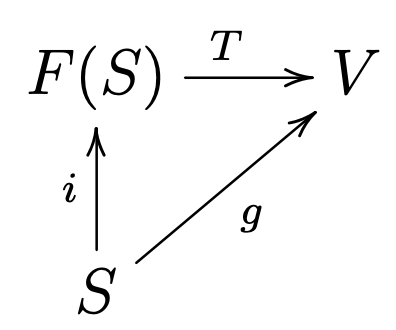
\includegraphics[scale=0.5]{ra_hw11_4}
\end{center}

\end{enumerate}

\end{proposition}

\begin{proof}

\begin{enumerate}[(a)]

\item We will check that sums and scalar multiples preserve the quality of vanishing at all but finitely many \(s\). 

For sums, observe that for \(f, g \in \bigoplus_{s \in S} V_s \) we have \((f+g)(s) = f(s) + g(s)\). By definition \(f(s)\) and \(g(s)\) both equal 0 for all but finitely many \(s \in S\); therefore the same is true for \(f(s) +g(s)\) and \((f+g)(s)\). 

For scalar multiplication, since for \(f \in \bigoplus_{s \in S} V_s \) we have \((cf)(s) = cf(s)\) and \(f(s)\) equals 0 for all but finitely many \(s \in S\), the same is true for \(cf(s)\) for any scalar \(c\) and therefore for \((cf)(s)\).

\item For \(f \in V_s \bigoplus V_t\), let \(f(s) = v\) and \(f(t) = w\) and define the linear map to \(V_s \times V_t \) by \(f \mapsto (f(s), f(t)) = (v,w)\). Observe that this map is linear because \(cf \mapsto ((cf)(s), (cf)(t)) = (c(f(s)), c(f(t))) = c(f(s), f(t)) = c(v,w)\) and for \(g\) satisfying \(g(s) = v'\) and \(g(t) = w'\) we have \(f + g \mapsto ((f(s) ,  f(t)) +( g(s),  g(t)) = (v, w) + (v', w') = (v + v', w + w')\). Note also that all of these mappings are bijective.

\item For \(f \in F(S)\), define \(T(f)\) to be the element of \(V\) given by \(\sum_{s \in S} f(s) g(s)\) (recall that \(f(s) \in \mathbb{R}\) and \(g(s) \in V\)). Observe that since \(f(s) =0\) for all but finitely many \(s\), \(\sum_{s \in S} f(s) g(s)\) is finite. We see that \(T\) is linear since

\[
T(cf) =  \sum_{s \in S} (cf)(s) g(s) =  \sum_{s \in S} cf(s) g(s) = c \sum_{s \in S} f(s) g(s) = cT(f)
\]

and for another \(f' \in F(S)\)

\[
T(f + f') = \sum_{s \in S} (f + f')(s) g(s) = \sum_{s \in S} [f(s)  + f'(s)] g(s) = \sum_{s \in S} f(s) g(s) + \sum_{s \in S} f'(s) g(s) = T(f) + T(f').
\]

Then the diagram commutes because for any \(s \in S\)

\[
( T \circ i)(s) = \sum_{s' \in S} i(s)(s') g(s) = \sum_{s' \in S, s' \neq s} 0 \cdot g(s) + 1 \cdot g(s) = g(s) .
\]

Now we will show uniqueness. Suppose \(T\) and \(T'\) are two linear maps such that the diagram commutes, so we have \(T(i(s)) = g(s) = T'(i(s))\). Let \(f \in F(S)\). Observe that

\[
f(s) = \sum_{s' \in S} i(s)(s') f(s) = \sum_{s' \in S, f(s') \neq 0} i(s)(s') f(s) ,
\]

which is a finite sum by the requirement that \(f(s) = 0\) for all but finitely many \(s \in S\). Now (using the linearity of \(T\) and \(T'\))

\begin{align*}
T(f(s)) & = T \left( \sum_{s' \in S, f(s') \neq 0} i(s)(s') f(s) \right) 
\\ & = \sum_{s' \in S, f(s') \neq 0} T \left(  i(s)(s') f(s) \right) 
\\ & = \sum_{s' \in S, f(s') \neq 0} f(s) T \left(  i(s)(s')  \right)
\\ & = \sum_{s' \in S, f(s') \neq 0} f(s) g(s) 
\\ & = \sum_{s' \in S, f(s') \neq 0} f(s) T' \left(  i(s)(s')  \right)
\\ & = \sum_{s' \in S, f(s') \neq 0} T' \left(  i(s)(s') f(s) \right) 
\\ & = T' \left( \sum_{s' \in S, f(s') \neq 0} i(s)(s') f(s) \right) 
\\ & = T'(f(s)).
\end{align*}


Therefore \(T(f) = T'(f)\), showing uniqueness.

\end{enumerate}

\end{proof}

Part (c) of Proposition \ref{ra.hw11.prob.4} shows that any function \(g\) from a set \(S\) to a vector space \(V\) can be extended linearly in a unique way to a linear transformation defined on \(F(S) := \oplus_{s \in S} \mathbb{R}\), the vector space of formal linear combinations of elements of \(S\).

\begin{definition}[Quotient Vector Space]\label{ra.def.quot.vect}

Let \(V\) be a vector space and let \(W\) be a subspace of \(V\). Define an equivalence relation on \(V\) by stating that \(v_1 \sim v_2\) if \(v_1 - v_2 \in W\). Let \(V/W\) denote the set of equivalence classes under this relation (see Definition \ref{ra.def.equiv}). The space \(V/W\) is called a \textbf{quotient vector space}.

If \(v \in V\), let \([v]\) denote its equivalence class. For two elements \(\alpha, \beta\) of \(V/W\), define \(\alpha + \beta\) to be \([v_1 + v_2]\) where \(\alpha = [v_1]\) and \(\beta = [v_2]\). Also, for \(c \in \mathbb{R}\), define \(c \alpha\) to be \([cv]\) where \(\alpha = [v]\).

\end{definition}

\begin{proposition}

The quotient vector space \(V/W\) satisfies the vector space axioms under the above definitions of addition and scalar multiplication. Also, if \(V\) has dimension \(n\) and \(W\) has dimension \(m\), then \(V/W\) has dimension \(n-m\).

\end{proposition}

\begin{proposition}[Math 425b Homework 12 problem]

\(\alpha + \beta\) and \(c \alpha\) as defined in Definition \ref{ra.def.quot.vect} are well-defined (i.e., independent of the choice of \(v_1\) and \(v_2\) representing \(\alpha\) and \(\beta\)).

\end{proposition}

\begin{proof}

Let \(v_1, v_1', v_2, v_2' \in V\) and let \(c \in \mathbb{R}\). Suppose that \(v_1 \sim v_1'\) and \(v_2 \sim v_2'\); that is, \(v_1 - v_1' \in W\) and \(v_2 - v_2' \in W\). Since \(W\) is a subspace of \(V\) (and therefore a vector space), it is closed under addition, so \(v_1 - v_1' + v_2 - v_2' \in W\). It also satisfies associativity of addition, so \((v_1 + v_2) - (v_1' + v_2') \in W\). Therefore \((v_1 + v_2) \sim (v_1' + v_2')\).

Next, observe that for any \(w \in W\), we have \(cw \in W\). Therefore \(c(v_1 - v_1') \in W\), which means \(c v_1 - c v_1' \in W\) (and \(c v_1 \sim c v_1'\)) by distributivity of scalar multiplication with respect to vector addition. Since these statements would be true for any \(\tilde{v}_1, \tilde{v}_1' \in \alpha\), \(\tilde{v}_2, \tilde{v}_2' \in \beta\), or \(c \in \mathbb{R}\), this shows that \(\alpha + \beta\) and \(c \alpha\) are well-defined.

\end{proof}

\begin{proposition}[Math 425b Homework 12 problem]

Let \(V\) be a vector space and let \(W\) be a subspace of \(V\). Let \(Z\) be another vector space and let \(f: V \to Z\) be a linear map such that \(f(w) = 0\) for all \(w \in W\). Let \(p: V \to V/W\) denote the linear map sending \(v \to [v]\). Then there exists a unique linear map \(g: V/W \to Z\) such that \(f = g \circ p\).

\end{proposition}

\begin{proof}

First we will show existence. Define \(g([v]) := f(v)\). To see that this is well-defined, consider another \(v' \in V\) such that \(v - v' \in W\); that is, \(v \sim v'\). Observe that \( f(v) - f(v') = f(v - v') = 0\) (by assumption that \(f(w) = 0\) for all \(w \in W\)), and since \([v] = [v']\), \(g([v]) - g([v']) = g([v]) - g([v]) =0\). Now consider an arbitrary \(v' \in V\) such that \(v - v' \notin W\). Note that \(f(v + v') = f(v) + f(v')\), and from Exercise 1, we have \([v] + [v'] = [v + v']\), so \(g([v + v']) = g([v]) + g([v'])\). Finally, for any \(c \in \mathbb{R}\) we have \(f(cv) = c f(v)\), and since from Exercise 1 we have \([cv]= c[v]\), we have \(g([cv]) = g(c[v]) = cg([v])\) by linearity of \(g\).

Now we will show uniqueness. Note that any \(\alpha \in V/W\) is equal to \([v] = p(v)\) for some \(v \in V\). Consider two maps \(g\) and \(\tilde{g}\) that make the diagram commute; that is, \(g([v']) = f(v')\) and \(\tilde{g}([v']) = f(v')\) for any \(v' \in V\).. Then for any \(\alpha \in V/W\), we have \(g(\alpha) = g([v]) = f(v) = \tilde{g}([v]) =\tilde{g}(\alpha)\). 

\end{proof}

Let \(V\) and \(W\) be vector spaces over \(\mathbb{R}\). Consider the free vector space \(F(V \times W)\) (see Definition \ref{ra.def.free.vector.space}). It is the set of functions \(f: V \times W \to \mathbb{R}^2 \). \(F(V \times W)\) is the vector space of all linear combinations of elements of \(V \times W\). The elements of \(V \times W\) form a basis for \(F(V \times W)\) by definition.

Given an element \((v,w) \in V \times W\), we view \((v,w)\) as an element of \(F(V \times W)\) via the inclusion map \(i: V \times W \to F(V \times W)\). Any element of \(F(V \times W)\) is a finite linear combination of such elements \((v,w)\).

Note that \(F(V \times W)\) disregards the vector space structures on \(V \) and \(W\), and just treats \(V \times W\) as the set of ordered pairs \((v,w)\) where \(v \in V\) and \(w \in W\). For example, if \(v \neq 0 \in V\), then \((v, 0)\) and \((2v, 0)\) are linearly independent in \(F(V \times W)\), even though \(v\) and \(2v\) are not linearly independent in \(V\).

\begin{definition}[\textbf{Tensor product}]\label{ra.def.tens.prod}

Let \(S\) be the subset of \(F(V \times W)\) consisting of the following elements:

\begin{itemize}

\item \((v,w) + (v', w) - (v+ v', w)\) for all \(v, v' \in V\) and \(w \in W\).

\item \((v,w) + (v', w) - (v, w + w')\) for all \(v  \in V\) and \(w, w' \in W\).

\item \(c(v,w) - (cv, w)\) for all \(v \in V\), \(w \in W\), and \(c \in \mathbb{R}\).

\item \(c(v,w) - (v, cw)\) for all \(v \in V\), \(w \in W\), and \(c \in \mathbb{R}\).

\end{itemize}

Define

\[
V \otimes W := \frac{F(V \times W)}{\operatorname{span}(S)}.
\]

That is, for \(f_1: V \times W \to \mathbb{R}^2 \in F( V \times W)\) and \(f_2: V \times W \to \mathbb{R}^2 \in F( V \times W)\), for an equivalence relation defined as \(f_1 \sim f_2 \) if \(f_1 - f_2 \in \operatorname{span}(S)\), \(V \otimes W\) is the quotient vector space consisting of the set of equivalence classes under this relation. In particular, if we view \((v,w)\) as an element of \(F(V \times W)\) via the inclusion map \(i: V \times W \to F(V \times W)\) (recall Definition \ref{ra.def.free.vector.space}), we can characterize the equivalence relation by \((v_1, w_1) \sim (v_2, w_2) \) if \((v_1, w_1) - (v_2, w_2) \in \operatorname{span}(S)\). Then \(V \otimes W\) is the quotient vector space consisting of the set of equivalence classes under this relation.

%\(V \bigotimes W := \frac{F(V \times W)}{\operatorname{span}(S)}\) is the set of equivalence classes on \(F(V \times W)\) where \((v_1 \times w_1) \sim (v_2 \sim w_2)\) if \((v_1 \times w_1)  -  (v_2 \times w_2) \in \operatorname{span}(S)\). 


Given an element \((v,w)\) of \(F(V \times W)\), its class \([(v,w)]\) in the quotient space \(V \otimes W\) will be denoted by \(v \otimes w\). Note that not every element of \(V \otimes W\) can be written as \(v \otimes w\) for some \(v \in V\) and \(w \in W\) (since not every function \(f: V \times W \to \mathbb{R}^2\) can be expressed as the inclusion map of a single \((v,w) \in V \times W\)). Elements like \(v \otimes w\) are called \textbf{pure tensors}. In general, an element of \(V \otimes W\) is a linear combination of pure tensors.

See also Section 4.1 of \citet{spivak1971calculus} (p. 88 of pdf, p. 75 of book).

\end{definition}

\begin{example}\label{ra.ex.tens.prod.zero}

The tensor product of zero copies of \(\mathbb{R}^n\) is defined to be \(\mathbb{R}\). (This  is relevant later in the dimensions of spaces of alternating multilinear functionals.)

\end{example}


\begin{definition}[\textbf{Bilinear maps; also in Section 5.2 of \citet{pugh2015real}, p. 297 of pdf, p. 287 of book}]\label{ra.def.bilinear}

Let \(V, W, Z\) be vector spaces over \(\mathbb{R}\). A map \(f: V \times W \to Z\) is said to be \textbf{bilinear} if 

\begin{itemize}

\item \(f(v + cv', w) = f(v, w) +  c f(v', w)\) for all \(v, v' \in V\), \(w \in W\), and \(c \in \mathbb{R}\).

\item \(f(v , w + cw') = f(v, w) +  c f(v, w')\) for all \(v \in V\), \(w, w' \in W\), and \(c \in \mathbb{R}\).

\end{itemize}

For a generalization of this concept, see multilinear maps (Definition \ref{ra.def.multilinear}).

\end{definition}

\begin{proposition}[Math 425b Homework 12 Problem 3] 

The map \(\pi: V \times W \to V \otimes W\) sending \((v,w)\) to \(v \otimes w\) is bilinear.

\end{proposition}

\begin{proof}

We will show that \(\pi(v + cv', w) = \pi(v, w) + c \pi(v', w)\). Let \(c \in \mathbb{R}\), \(v, v' \in V\), \(w \in W\). Note that since \(c v' \in V\), we have

\begin{align*}
(v+cv', w) - (v,w) - c(v',w)  & = (v+cv', w) - (v, w) -  c(v', w) - (cv', w)     + (cv', w) 
\\ & = - \underbrace{(v, w) + (cv', w) -(v+cv', w) }_{\in S} -  \underbrace{ c(v', w) - (cv', w) }_{\in S}.
\end{align*}

Therefore \((v+cv', w) - (v,w) - c(v',w)\) is in the span of \(S\). That means it is in the equivalence class \([0]\), so \(0 = \pi\left( (v+cv', w) - (v,w) - c(v',w) \right) = \pi(v + cv', w) -  \pi(v, w) - c \pi(v', w)  \iff \pi(v + cv', w) = \pi(v, w) + c \pi(v', w)\). The other equation is similar.
 
\end{proof}

Tensor products have a ``universal property:" roughly speaking, a bilinear map from \(V \times W\) to \(Z\) is the same as a linear map from \(V \otimes W\) to \(Z\).


\begin{proposition}[Math 425b Homework 12 Problem 4]

Let \(V, W, Z\) be vector spaces over \(\mathbb{R}\). Let \(f: V \times W \to Z\) be a bilinear map. Let \(\pi: V \times W \to V \otimes W\) be defined by \(\pi(v,w) := v \otimes w\). Then there exists a unique linear map \(g: V \otimes W \to Z\) such that \(f = g \circ \pi\).

\end{proposition}

Using this universal property, we have \(V \otimes W \cong W \otimes V\) for any vector spaces \(V\) and \(W\). Other standard properties also follow, like \((V \otimes W) \otimes Z \cong V \otimes (W \otimes Z)\). One can also deduce relations like \(V \otimes(W_1 \oplus W_2) \cong (V \otimes W_1) \oplus (V \otimes W_2)\); i.e., tensor products distributed over direct sums (up to isomorphism). The vector space \(\mathbb{R}\) acts as a ``unit" for the tensor product operations: for any \(V\), we have \(V \otimes \mathbb{R} \cong V\).

It follows that if \(V\) has dimension \(n\), so \(V \cong \mathbb{R}^n \cong \underbrace{\mathbb{R} \oplus \ldots \oplus \mathbb{R}}_{n \text{ terms}}\), and \(W\) has dimension \(m\), then

\[
V \otimes W \cong \underbrace{(\mathbb{R} \oplus \ldots \oplus \mathbb{R})}_{n \text{ terms}} \otimes \underbrace{(\mathbb{R} \oplus \ldots \oplus \mathbb{R})}_{m \text{ terms}},
\]

which expands out to \(nm\) copies of \(\mathbb{R}\). Thus, \(V \otimes W\) has dimension \(nm\). Concretely, if \(\{e_i\}\) forms a basis for \(V\) and \(\{f_j\}\) forms a basis for \(W\), then \(\{e_i \otimes f_j\}\) forms a basis for \(V \otimes W\) (see also Theorem 4-1 in \citet{spivak1971calculus}, p. 89 of pdf, p. 76 of book).

Mathematicians often define a vector to be an element of a vector space. Correspondingly, one can define a tensor as follows.

\begin{definition}[\textbf{Tensors}]\label{ra.def.tensor}

A \textbf{tensor of rank \(k\)} is an element of the vector space \(V_1 \otimes \cdots \otimes V_k\) for some \(k \geq 1\) (i.e., a tensor is a vector in the space \(V_1 \otimes \cdots \otimes V_k\)).

\end{definition}

Along with tensor products, another essential operation on vector spaces is the notion of the dual space (recall Definition \ref{ra.def.dual.space}). 

\begin{definition}[\textbf{Basis vectors for dual space; 425b Homework 13}]\label{ra.def.basis.dual}

If \(\{e_i\}\) is a basis for \(V\), define the linear functionals \(e_i^*: V \to \mathbb{R} \in V^*\) by 

\[
e_i^*(e_j) := \delta_{i,j} = \begin{cases}
1, & i = j, \\
0, & i \neq j,
\end{cases}
\] 

where \(V^*\) is the dual space of \(V\) (recall Definition \ref{ra.def.dual.space}).(Following the up/down notation mentioned below, one often write \(e^i\) instead of \(e_i^*\).) In Proposition \ref{ra.prop.basis.dual}, we show that these vectors are a basis for \(V^*\).

\end{definition}





\begin{remark}

In some contexts it is common to present tensors as being higher-dimensional analogues of vectors and matrices. If a vector is a one-dimensional array of numbers and a matrix is a two-dimensional array, a tensor of rank \(k\) should be a \(k\)-dimensional array. One can connect this view with tensors with Definition \ref{ra.def.tensor} as follows: given bases \(\{e_{i,j}\}_j\) for each \(V_i\), one gets a basis for \(V_1 \otimes \cdots \otimes V_k\) by taking tensor products of basis vectors as defined in Definition \ref{ra.def.tens.prod} (see Theorem 4-1 in \citet{spivak1971calculus}, p. 89 of pdf, p. 76 of book). An arbitrary element of \(V_1 \otimes \cdots \otimes V_k\) can be expanded as a linear combination of basis vectors; one has a unique coefficient \(c_{j_1, \ldots, j_k}\) on each basis vector \(e_{1, j_1} \otimes \cdots \otimes e_{k, j_k}\). One organizes these coefficients into an array of the appropriate dimensionality:

\begin{itemize}

\item For \(k=1\), the coefficients \(c_j\) form a one-dimensional array (vector),

\item For \(k=2\), the coefficients \(c_{j_1, j_2}\) form a two-dimensional array (matrix),

\item For \(k=3\), the coefficients \(c_{j_1, j_2, j_3}\) form a three-dimensional array (rank-3 tensor), etc.

\end{itemize}

Now that we have dual vector spaces, we often prefer to view a matrix as representing a linear transformation between vector spaces \(T: V \to W\) and then interpret this transformation as an element of \(W \otimes V^*\) (still a rank-2 tensor, but involving a dual on one of the factors).

\end{remark}

\begin{definition}[\textbf{Covariant tensors}]

Let \(V_1, \ldots, V_k\) be fixed vector spaces. An element \(x\) of \(V_1 \otimes \cdots \otimes V_k\) is called a \textbf{covariant tensor}. We write its coefficient on a basis vector \(e_{1, j_1} \otimes \cdots \otimes e_{k j_k}\) as \(x^{j_1 ,\ldots, j_k}\) (i.e., we use ``up indices").

\end{definition}

\begin{definition}[\textbf{Contravariant tensors}]

Let \(V_1, \ldots, V_k\) be fixed vector spaces. An element \(x\) of \(V_1^* \otimes \cdots \otimes V_k^*\) is called a \textbf{contravariant tensor}. We write its coefficient on the dual basis vector \(e^{1, j_1} \otimes \cdots \otimes e^{k j_k}\) as \(x_{j_1 ,\ldots, j_k}\) (i.e., we use ``down indices").

\end{definition}

In between these extreme cases, we have various types of \textbf{mixed tensors} whose coefficients have both up and down indices. 

\begin{remark}\label{ra.remark.up.index}

The up/down notation is part of ``Einstein notation," developed by Albert Einstein for use in relativity. Another part of the convention is to write only the coefficients and note the basis vectors they're multiplied by when specifying a tensor. For example,

\begin{itemize}

\item A vector \(x = \sum_i x^i e_i\) in \(V\) gets written as \(x^i\),

\item A dual vector \(x = \sum_i x_i e^i \in V^*\) gets written as \(x_i\),

\item A rank-2 covariant tensor \(\sum_{i,j} x^{i,j} e_i \otimes f_j\) in \(V \otimes W\) gets written as \(x^{i,j}\) where \(\{f_j\}\) is the given basis for \(W\),

\item A rank-2 mixed tensor \(\sum_{i,j} x_j^i e_i \otimes f^j\) in \(W \otimes V^*\) gets written as \(x_j^i\),

\item A rank-2 contravariant tensor \(\sum_{i,j} x_{i,j} e^i \otimes f^j\) in \(V^* \otimes W^*\) gets written as \(x_{i,j}\).

\end{itemize}

Often one will consider certain sums of these coefficients; the convention is that one sums over repeated indices (one must be up and the other down) and omits the sum symbol. For example, let \(a_j^i\) represent an element of \(W \otimes V^*\) (corresponding to a linear transformation \(T\) from \(V\) to \(W\); in fact, in the assumed bases, \(a_j^i\) is the usual matrix entry of \(T\) in row \(i\) and column \(j\)). Mathematically, we would write \(a_j^i\) as \(\sum_{i,j} a_j^i e_i \otimes f^j\). Let \(v^i\) represent a vector in \(V\); mathematically, we would write \(v^i\) as \(\sum_i v^i e_i\). Applying the transformation \(a-j^i\) to the vector \(v^i\) gives \(\sum_{i,j}a_j^i v^j f_i\) (a vector in \(W\)), and the convention is to write this vector as simply \(a_j^i v^j\) (the sum over \(j\) is implicit, as is the sum over \(i\) with the ``invisible" basis vectors \(f_i\)). You know this quantity represents a vector since it has one ``free' index \(i\) and this index is up.

\end{remark}

\begin{proposition}[\textbf{Math 425b Homework 13 Problem 1; similar to Theorem 4-1 in \citet{spivak1971calculus}, p. 89 of pdf, p. 76 of book, also Proposition 11.1 in \citet{lee2012introduction}}]\label{ra.prop.basis.dual}

Let \(V\) be a finite-dimensional vector space with basis \(\{e_i\}\). Define the linear functionals \(e_i^* \in V^*\)  by 

\[
e_i^*(e_j) := \delta_{i,j} = \begin{cases}
1, & i = j, \\
0, & i \neq j
\end{cases}
\]  

as in Definition \ref{ra.def.basis.dual}. The linear functionals \(\{e_i^*\}\) form a basis for \(V^*\). Further, \(V^*\) has the same dimension as \(V\).

Also, if \(V\) and \(W\) are finite-dimensional with bases \(\{e_i\}\) and \(\{f_j\}\), then the elements \(e_i \otimes f_j\) form a basis for \(V \otimes W\); in particular, the dimension of \(V \otimes W\) is the product of the dimensions of \(V\) and \(W\).

\end{proposition}

\begin{proof}

To show that \(\{e_i^*\}\) forms a basis for \(V^*\), we will show that the \(\{e_i^*\}\) are linearly independent and that they span \(V^*\). Let \(n := \left| \{e_i^*\} \right|=\operatorname{dim}(V)\). Since \(\{e_i\}\) is a basis for \(V\), for every \(v \in V\) there exists a unique \((c_1, \ldots, c_n) \in \mathbb{R}^n\) such that \(v = \sum_{i=1}^n c_i e_i\). Suppose for some \((c_1^*, \ldots, c_n^*) \in \mathbb{R}^n\) we have \(\sum_{j=1}^n c_j^* e_j^*(v) = 0\) for all \(v \in V\). Then for any \(v \in V\)

\[
0 = \sum_{j=1}^n c_j^* e_j^*(v) = \sum_{j=1}^n c_j^* e_j^* \left( \sum_{i=1}^n c_i e_i \right) = \sum_{j=1}^n c_j^*  \sum_{i=1}^n c_ie_j^* \left( e_i \right) =   \sum_{i=1}^n c_i^*c_ie_i^* \left( e_i \right) =   \sum_{i=1}^n c_i^*c_i
\]

(where the third equality follows from the fact that \(e_j^*\) is linear and the fourth equality follows from \(e_j^*(e_i) =0 \) for all \(j \neq i\)), which only holds for all \(v \in V\) if \((c_1^*, \ldots, c_n^*) = (0, \ldots, 0)\). Therefore the \(\{e_i^*\}\) are linearly independent. Next we will show that the \(\{e_i^*\}\) span \(V^*\). Let \(\phi: V \to \mathbb{R}\) be an arbitrary linear functional. We will show in particular that \(\phi(v) = \sum_{j=1}^n c_j^* e_j^*(v) \) for some \((c_1^*, \ldots, c_n^*) \in \mathbb{R}^n\) for any \(v =  \sum_{i=1}^n c_i e_i \in V\). We have

\begin{multline*}
\phi(v) = \phi \left(  \sum_{j=1}^n c_j e_j \right) = \sum_{j=1}^n c_j  \phi \left(  e_j \right) = \sum_{j=1}^n \phi(e_j) c_j   e_j^*\left(e_j  \right)  = \sum_{j=1}^n \phi(e_j)\sum_{i=1}^n c_i   e_j^*\left(e_i  \right) = \sum_{j=1}^n \phi(e_j) e_j^*\left(\sum_{i=1}^n c_i e_i  \right)
\\ = \sum_{j=1}^n \phi(e_j) \cdot e_j^*(v) = \sum_{j=1}^n c_j^* \cdot e_j^*(v)
\end{multline*}

where \((c_1^*, \ldots, c_n^*) = (\phi(e_1), \ldots, \phi(e_n))\).

Next we will show that if \(V\) and \(W\) are finite-dimensional with bases \(\{e_i\}\) and \(\{f_j\}\), then the elements \(e_i \otimes f_j\) form a basis for \(V \otimes W\); in particular, the dimension of \(V \otimes W\) is the product of dimensions of \(V\) and \(W\). We can write \(V\) as \(\mathbb{R} \oplus \cdots \oplus \mathbb{R}\), with \(n\) copies of \(\mathbb{R}\). Similarly, we can write \(W\) as \(\mathbb{R} \oplus \cdots \oplus \mathbb{R}\), with \(\operatorname{dim}(W)\) copies of \(\mathbb{R}\).

We will use the fact that if \(V_1, V_2, W\) are vector spaces and \(T_1: V_1 \to W, T_2, V_2 \to W\) are linear maps, there exists a unique linear map \(T: (V_1 \oplus V_2) \to W\) such that \(T((v_1,0)) = T_1(v_1)\) and \(T((0,v_2)) = T_2(v_2)\).

\end{proof}

\begin{proposition}[\textbf{Math 425b Homework 13 Problem 2}]\label{ra.tensors.prop.hw13.2}

Let \(V\) and \(W\) be vector spaces over \(\mathbb{R}\). Define a map \(T: V^* \times W^* \to (V \otimes W)^*\) that sends \((\phi, \psi) \in V^* \times W^*\) to \((v \otimes w) \mapsto \phi(v) \psi(w) \in (V \otimes W)^*\) (recall Definition \ref{ra.def.dual.space} for the definition of the dual spaces \(V^*\) and \(W^*\)). This map \(T\) is well-defined and bilinear (recall Definition \ref{ra.def.bilinear}), and thus induces a linear map \(V^* \otimes W^* \to (V \otimes W)^*\). Further, if \(V\) and \(W\) are finite-dimensional, this induced map is an isomorphism.

\end{proposition}

\begin{remark}\label{ra.rmk.multilinear.map}

The left side \( (V \otimes W)^*\) of the isomorphism in Proposition \ref{ra.tensors.prop.hw13.2} can be identified as the space of bilinear maps from \(V \times W\) to \(\mathbb{R}\). Proposition \ref{ra.tensors.prop.hw13.2} shows that this space of bilinear maps can also be described as \(V^* \otimes W^*\), when \(V\) and \(W\) are finite-dimensional. More generally, if all spaces \(V_i\) are finite-dimensional we can identify \(V_1^* \otimes \cdots \otimes V_n^*\) with the space of multlinear maps from \(V_1 \times \cdots \times V_n\) into \(\mathbb{R}\).

Even more generally, if all spaces \(V_i\) and \(W_j\) are finite-dimensional, we can identify \(V_1^* \otimes \cdots \otimes V_n^* \otimes W_1 \otimes \cdots \otimes W_m\) with the space of multlinear maps from \(V_1 \times \cdots \times V_n\) to \(W_1 \otimes \cdots \otimes W_n\). A special case is when \(n=m=1\); we can identify \(V^* \otimes W\) (or \(W \otimes V\)) with the space of linear maps from \(V\) to \(W\). 

\end{remark}

\subsection{Differential Forms (Section 5.8 of \citet{pugh2015real}; Chapter 10 of \citet{rudin1976principles})}\label{ra.5.8.pugh}

\begin{definition}[\textbf{Multilinear functionals; Section 5.9 of \citet{pugh2015real}}]\label{ra.def.multilinear}

A map \(\beta:  \underbrace{\mathbb{R}^n \times \ldots \times \mathbb{R}^n}_{k \text{ times}} \to \mathbb{R}\) which is linear in each vector variable separately is a \textbf{\(k\)-multilinear functional.} That is, for \(i \in [k]\) we have

\[
\beta(x_1, \ldots, x_i + cx_i', \ldots, x_k) = \beta(x_1, \ldots, x_i  \ldots, x_k)  + c \beta(x_1, \ldots, x_i', \ldots, x_k) .
\]

A bilinear map is a 2-multilinear map; see Definition \ref{ra.def.bilinear}.

\end{definition}

\begin{definition}[\textbf{Symmetric groups and permutations}]\label{ra.def.symm.perm}

We call the set of all permutations of \([k]\) (of size \(k!\)) the \textbf{symmetric group on \(k\)} and denote it by \(S_k\). We refer to its elements as \(\sigma \in S_k\). The number of transpositions modulo 2 in any factorization of \(\sigma\) into transpositions is well-defined and denoted by \(\operatorname{sgn}(\sigma)\).

See Section \ref{abs.alg.sec.sym}.

\end{definition}

\begin{definition}[\textbf{Alternating multilinear functionals; Section 5.9 of \citet{pugh2015real}, Section 4.1 of \citet{spivak1971calculus} (p. 91 of pdf, p. 78 of book)}]

A \(k\)-multilinear functional \(\beta: \mathbb{R}^n \times \ldots \times \mathbb{R}^n \to \mathbb{R}\) is \textbf{alternating} if for each permutation \(\sigma \in S_k\) we have

\[
\beta(v_1, \ldots, v_k) = \operatorname{sgn}(\sigma) \beta(v_{\sigma(1)}, \ldots, v_{\sigma(k)}).
\]

The set of alternating \(k\)-linear forms is a vector space. In particular, we denote by \(\operatorname{Alt}_k(\mathbb{R}^n, \mathbb{R})\) the vector space of multilinear maps \(\alpha: \underbrace{\mathbb{R}^n \times \cdots \times \mathbb{R}^n}_{k \text{ times}} \to \mathbb{R}\) with 

\[
\alpha (v_1 , \ldots, v_{i+1}, v_i, \ldots, v_k) = - \alpha(v_1, \ldots, v_i, v_{i+1}, \ldots, v_k)
\]

for \(1 \leq i \leq k\). (In \citet{spivak1971calculus}, this space is denoted by \(\Lambda^k(V)\).)

\end{definition}

\begin{example}\label{ra.ex.1.multi.ex}

The set of 1-multilinear functionals is the set of linear functionals from \(\mathbb{R}^n \to \mathbb{R}\).

\end{example}

\begin{example}\label{ra.ex.2.multi.ex}

The set of 2-multilinear functionals is the set of bilinear functionals from \(\mathbb{R}^n \times \mathbb{R}^n \to \mathbb{R}\) satisfying 

\[
\beta(v, w) = - \beta(w, v)
\]

for all \(v, w \in \mathbb{R}^n \).

\end{example}

\begin{example}\label{ra.ex.0.multi.ex}

The set of 0-multilinear functionals is \(\mathbb{R}\).

\end{example}

\begin{definition}[\textbf{Differential \(k\)-forms; from Math 425B Homeworks 13 and 14}]\label{ra.def.diff.k.forms}

 A \textbf{differential \(k\)-form} on \(U \subset \mathbb{R}^n\) is a function \(\alpha: U \to \operatorname{Alt}_k(\mathbb{R}^n, \mathbb{R})\).



From Remark \ref{ra.rmk.multilinear.map}, \(\operatorname{Alt}_k(\mathbb{R}^n, \mathbb{R})\) can be viewed as a subspace of \(\underbrace{(\mathbb{R}^n)^* \otimes \cdots \otimes (\mathbb{R}^n)^*}_{k \text{ times}}\) (recall Definition \ref{ra.def.tens.prod} for the definition of the tensor product \(\otimes\), and recall Definition \ref{ra.def.dual.space} for the definition of the dual space \((\mathbb{R}^n)^*\)). So a differential \(k\)-form is a particular type of rank-\(k\) contravariant tensor field on \(U\) (namely one that satisfies the ``alternating property" at each point). While this perspective is not strictly speaking necessary to define differential \(k\)-forms, it is very useful when defining wedge products (see Definition \ref{ra.def.wedge.prod} and \ref{ra.def.wedge.prod.gen}).

\(C^r\) regularity for differential \(k\)-forms can be defined by looking at their coordinates in any basis for the finite-dimensional vector space \(\operatorname{Alt}_k(\mathbb{R}^n, \mathbb{R})\) (independently of the choice of basis). That is, we say that \(\alpha\) is of class \(C^r\) if its coordinates in the standard basis of \((\mathbb{R}^n)^* \otimes \cdots \otimes (\mathbb{R}^n)^*\) (equivalently, any basis for this vector space) are \(C^r\) functions from \(U\) to \(\mathbb{R}\).

That is, a differential \(k\)-form on \(U\) is a function \(\alpha\) from \(U\) to \( \underbrace{(\mathbb{R}^n)^* \otimes \cdots \otimes (\mathbb{R}^n)^*}_{k \text{ times}}\) which is alternating in the following sense: viewing \(\alpha(p) \in (\mathbb{R}^n)^* \otimes \cdots \otimes (\mathbb{R}^n)^*\) as an element of \((\mathbb{R}^n \otimes \cdots \otimes \mathbb{R}^n)^*\) \textbf{by the below Propositions [which?]} (i.e., a multilinear map from \(\mathbb{R}^n \times \cdots \times \mathbb{R}^n \) to \(\mathbb{R}\)), the map \(\alpha(p)\) is alternating in the sense that for all \(k\)-tuples \((v_1, \ldots, v_k)\) of vectors in \(\mathbb{R}^n\), we have

\[
\alpha(p)(v_1 \otimes \cdots \otimes v_i \otimes v_{i+1} \otimes \cdots \otimes v_k) = -\alpha(p)(v_1 \otimes \cdots \otimes v_{i+1}  \otimes v_i  \otimes \cdots \otimes v_k) 
\]

for any \(i\) with \( 1 \leq i \leq k-1\). 



\end{definition}



\begin{example}\label{ra.ex.0.multi.form.ex})

Let \(U \subset \mathbb{R}^n\) be open. Since \(\operatorname{Alt}_0(\mathbb{R}^n, \mathbb{R}) = \mathbb{R}\) (see Example \ref{ra.ex.0.multi.ex}), a \textbf{differential 0-form} on \(U\) is a function \(f: U \to \mathbb{R}\).
\end{example}

\begin{example}\label{ra.ex.1.multi.form.ex}

Let \(U \subset \mathbb{R}^n\) be open. A \textbf{differential 1-form} on \(U\) is a function \(\alpha: U \to (\mathbb{R}^n)^*\). Given any basis \(\{\phi_1, \ldots, \phi_n\}\) for \((\mathbb{R}^n)^*\), we can write \(\alpha(p) = a_1(p) \phi_1 + \ldots + a_n(p) \phi_n\), where \(a_1, \ldots, a_n\) are functions from \(U\) to \(\mathbb{R}\). We say that \(\alpha\) is of class \(C^r\) (\(1 \leq r \leq \infty\)) if all the functions \(a_i\) are of class \(C^r\). Since changes of basis on \(\mathbb{R}^n\) are \(C^\infty\) (even linear) functions, this notion is independent of the choice of basis \(\{\phi_1, \ldots, \phi_n\}\).


Since \(\operatorname{Alt}_1(\mathbb{R}^n, \mathbb{R})\) is the set of linear functionals from \(\mathbb{R}^n \to \mathbb{R}\) (see Example \ref{ra.ex.1.multi.ex}), we can also say that a differential 1-form \(\alpha\), evaluated at a point \(p \in U\), gives a linear functional \(\alpha(p)\) from \(\mathbb{R}^n \) to \(\mathbb{R}\).

Also, any 1-form \(\alpha\) on \([a,b]\) is \(f(t) dt\) for some function \(f\).

Given a basis for \(\mathbb{R}^n\) (in particular, the standard basis), one can identify differential 1-forms on \(U\) with \textbf{vector fields} on \(U\) (see Definition \ref{ra.def.vector.field}); i.e., functions from \(U\) to \(\mathbb{R}^n\) (rather than \((\mathbb{R}^n)^*\)) (see Remark \ref{ra.remark.riemannian.metric}).

\end{example}

\begin{definition}[\textbf{Differential 1-forms; from \citet{pugh2015real} Section 5.8, p. 337 of pdf, p. 327 of book}]

A \textbf{differential 1-form} is a function that sends paths to real numbers and which can be expressed as a path integral (for example, \(f \ dx + g \ dy\) is a 1-form).

\end{definition}

\begin{example}[\textbf{Example from \citet{pugh2015real} Section 5.8, p. 337 of pdf, p. 327 of book}]\label{ra.ex.1.form.int.pugh}

Consider a path integral as its defined in calculus:

\begin{equation}\label{ra.pugh.path.int.examp.diff.form}
\int_C (f \ dx + g\ dy) = \int_0^1 f(x(t), y(t)) \deriv{x(t)}{t} dt + \int_0^1  g(x(t), y(t)) \deriv{y(t)}{t} dt,
\end{equation}

where \(f\) and \(g\) are smooth real-valued functions of \((x,y)\) and \(C\) is a smooth path parameterized by \((x(t), y(t))\) as \(t\) varies on \([0,1]\). Taking the dual approach of differential forms, we will think of the integral as a number that depends on the path \(C\). What property of \(C\) does the differential 1-form \(f \ dx + g\ dy\) measure?

Consider the case \(f(x,y)= 1\) and \(g(x,y)= 0\). Then the path integral \eqref{ra.pugh.path.int.examp.diff.form} is

\[
\int_C dx = \int_0^1 \deriv{x(t)}{t} dt = x(1) - x(0),
\]

the ``net x-variation" of the path \(C\). In functional notation, we can write \(dx: C \mapsto x(1) - x(0)\), so \(dx\) assigns to  each path \(C\) its net \(x\)-variation. Similarly, \(dy\) assigns  to each path its net \(y\)-variation.

For a general  \(f \ dx\), the function \(f\) ``weights" \(x\)-variation. If the path \(C\) passes through a region in which \(f\) is large, its \(x\)-variation is magnified accordingly, and the integral \(\int_C f \ dx\) reflects the net \(f\)-weighted \(x\)-variation of \(C\). Similarly, \(g \ dy\) assigns a path to its net  \(g\)-weighted variation, and the 1-form \(f \  dx + g\ dy\) assigns to \(C\) the sum of the two variations. See Figure \ref{ra_fig_1form_fig}.

\begin{figure}[htbp]
\begin{center}
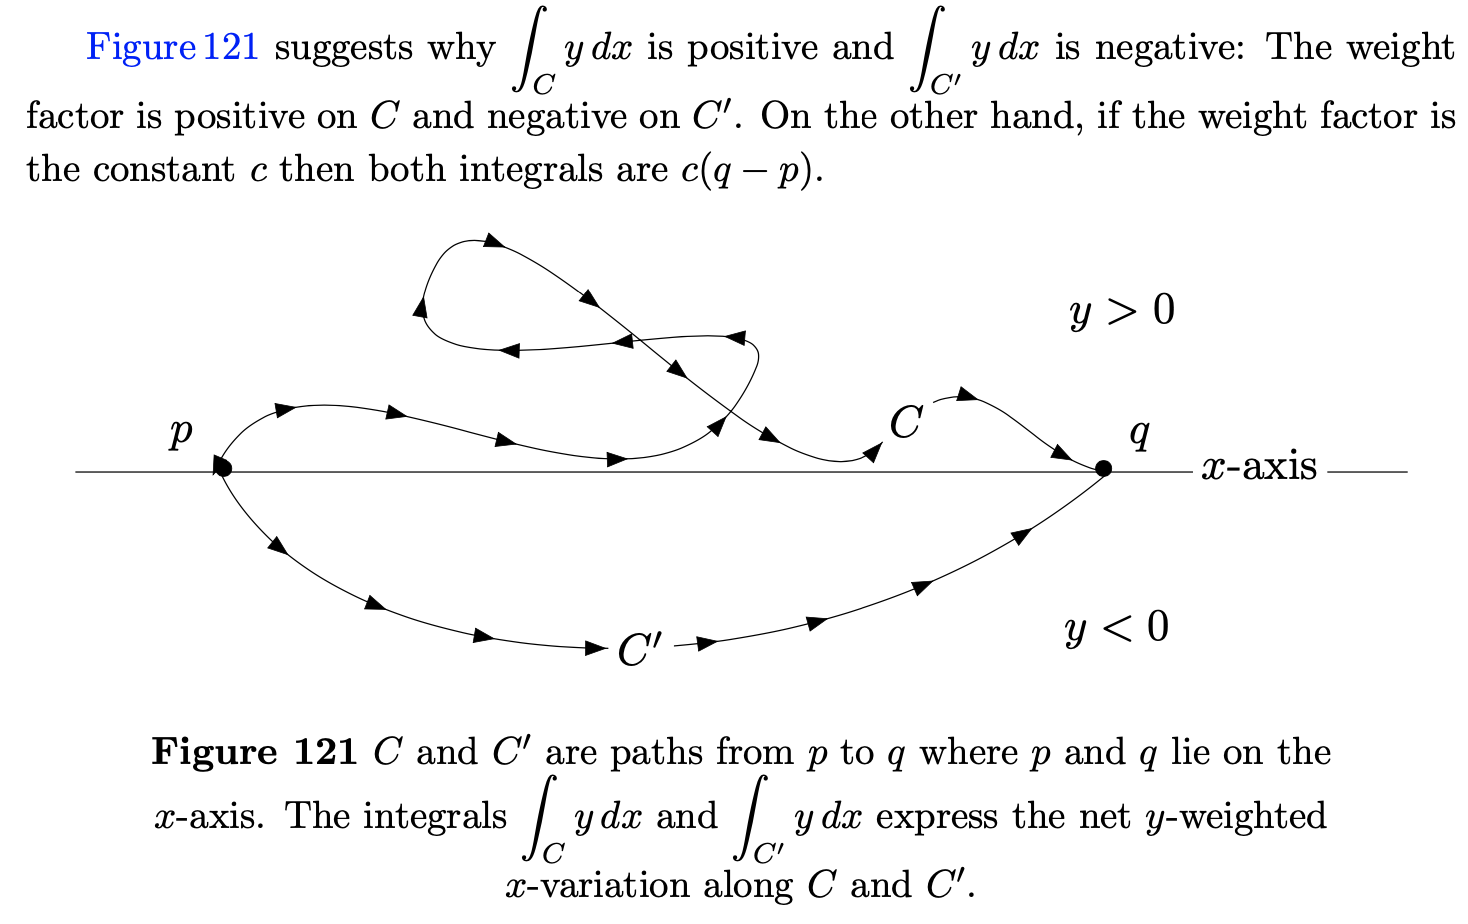
\includegraphics[scale=0.5]{ra_fig_1form}
\caption{Figure 121 from \citet{pugh2015real}, illustrating 1-forms.}
\label{ra_fig_1form_fig}
\end{center}
\end{figure}


\end{example}

\begin{example}\label{ra.ex.2.multi.form.ex}

Note that \(\operatorname{Alt}_2(\mathbb{R}^n, \mathbb{R})\) is the set of bilinear functionals from \(\beta: \mathbb{R}^2 \to \mathbb{R}\) satisfying \(\beta(v, w) = - \beta(w, v)\) for all \((v,w) \in \mathbb{R}^2\) (see Example \ref{ra.ex.2.multi.ex}). Therefore a differential 2-form \(\alpha\), evaluated at a point \(p \in U\), gives a bilinear map \(\alpha(p)\) from \(\mathbb{R}^n \times \mathbb{R}^n\) to \(\mathbb{R}\) such that \(\alpha(p)(v, w) = - \alpha(p)(w,v)\) for all \(v, w \in \mathbb{R}^n\).

\end{example}

There are four fundamental operations on differential forms that we need to understand.

\begin{enumerate}

\item \textbf{Exterior derivative:} if \(\alpha\) is a \(k\)-form (say \(C^\infty\)), then we have a \((k+1)\)-form \(d \alpha\). This operation will generalize the gradient (Remark \ref{ra.remark.riemannian.metric}), curl, and divergence operations (Proposition \ref{ra.42b.hw14.prob.5}). See Definition \ref{ra.def.ext.deriv.0} for the exterior derivative of a 0-form (also called a differential) and Definition \ref{ra.def.ext.deriv.k} for the exterior derivative of a \(k\)-form.

\item \textbf{Wedge product:} if \(\alpha\) is a \(k\)-form and \(\beta\) is an \(\ell\)-form, then we have a \((k+\ell)\)-form \(\alpha \wedge \beta\) (this operation will generalize the cross product of vectors in \(\mathbb{R}^3\)). See Definition \ref{ra.def.wedge.prod} and Definition \ref{ra.def.wedge.prod.gen}.



\item \textbf{Pullback:} if \(\alpha\) is a \(k\)-form on \(U\) and \(F: V \to U\) is smooth where \(V \subset \mathbb{R}^m\) is open (for some \(m\)), then we have a \(k\)-form \(F^*(\alpha)\) on \(V\). (See also Definition \ref{ra.def.pullback.1.form} below for the definition of pullbacks of 1-forms and Definition \ref{ra.def.pullbacks.gen} for the general definition.)



\item \textbf{Integration:} if \(\alpha\) is a \(k\)-form on a \(k\)-dimensional cube \([0,1]^k \subset \mathbb{R}^k\) (it's okay that this isn't an open set although \(\alpha\) should at least be right-continuous), we have a real number \(\int_{[0,1]^k} \alpha\). (We can also integrate on more general rectangular sets than just \([0,1]^k\).) Combined with pullbacks, this operation will let us generalize line integrals and surface integrals. (See also Example \ref{ra.ex.1.form.int.pugh}.)

\begin{example}

Integration of zero-forms on \(\mathbb{R}^0\) is just evaluation at the unique point \(0 \in \mathbb{R}^0\).

Also, any 1-form \(\alpha\) on \([a,b]\) is \(f(t) dt\) for some function \(f\), and if \(f\) is smooth or just Riemann integrable, we can just define \(\int_{[a,b]} \alpha := \int_a^b f(t) dt\) as usual.

\end{example}

\end{enumerate}

Now we will consider less trivial operations than just 0-forms and 1-forms. We will start by studying the exterior derivative \(df\) of a zero-form \(f\) (also known as the differential of \(f\)), closely related to the gradient of \(f\).

\begin{definition}[\textbf{Exterior derivative of a 0-form (differential)}]\label{ra.def.ext.deriv.0}

Let \(U \subset \mathbb{R}^n\) be open and let \(f: U \to \mathbb{R}\) be a smooth function (0-form). Define a differential 1-form \(df\) by the equation

\[
df(p) = (Df)_p.
\]

(In other words, \(df\) is just the Jacobian \(Df\) (see Theorem \ref{ra.thm.jacobian}), which at a point \(p\) gives a linear map from \(\mathbb{R}^n\) to \(\mathbb{R}\).) Basically the transpose of the gradient. See also Definition \ref{ra.def.ext.deriv.k} for the exterior derivative of a \(k\)-form.

\end{definition}

\begin{proposition}[\textbf{Math 425b Homework 13 Problem 3}]\label{ra.425b.hw13.3}

Let \(\{e_1, \ldots, e_n\}\) be the standard basis vectors of \(\mathbb{R}^n\) and let \(\{e_1^*, \ldots , e_n^*\}\) be their dual basis vectors (see Definition \ref{ra.def.basis.dual}). Let \(f\) be as above; prove that

\[
df = \pderiv{f}{x^1}e_1^* + \ldots + \pderiv{f}{x^n}e_n^*.
\]

(we use ``up indices" \(x^i\) rather than ``down indices" \(x_i\) to match the physics conventions; a physicist may write \(df\) as \(\pderiv{f}{x^i}\) or even as \(\partial_i f\), which is a 1-form since the \(i\) index is down, because up indices in a denominator are down. See Remark \ref{ra.remark.up.index}.)

\end{proposition}

\begin{proof}

It is enough to show that \(df(p)(e_i) = \pderiv{f}{x^i}(p) \) for each \(i\) and each \(p \in U\). Since for each \(p \in U\) we have

\[
(DF)_p =\begin{bmatrix} \pderiv{F_1}{x_1}(p) & \cdots & \pderiv{F_1}{x_n}(p) \\
\vdots & \ddots & \vdots \\
\pderiv{F_m}{x_1}(p) & \cdots & \pderiv{F_m}{x_n}(p) \end{bmatrix},
\]

it holds that

\[
(DF)_pe_i  = \begin{bmatrix} \pderiv{F_1}{x_1}(p) & \cdots & \pderiv{F_1}{x_n}(p) \\
\vdots & \ddots & \vdots \\
\pderiv{F_m}{x_1}(p) & \cdots & \pderiv{F_m}{x_n}(p) \end{bmatrix} \begin{bmatrix} 0 \\ \vdots \\ 1 \\ \vdots \\ 0 \end{bmatrix}= \sum_{j=1}^n \pderiv{F_i}{x_j}(p)=  \pderiv{f}{x^i}(p) 
\]

for each \(i\). Therefore \(df(p)(e_i) = \pderiv{f}{x^i}(p) \) for each \(i\) and each \(p \in U\).
\end{proof}

\begin{remark}[\textbf{From 425b Homework 13 Problem 4; Theorem 4-7 in \citet{spivak1971calculus} (p. 102 of pdf, p. 89 of book)}]\label{ra.remark.riemannian.metric}

Given a basis for \(\mathbb{R}^n\) (in particular, the standard basis), one can identify differential 1-forms on \(U\) with \textbf{vector fields} on \(U\) (see Definition \ref{ra.def.vector.field}); i.e., functions from \(U\) to \(\mathbb{R}^n\) (rather than \((\mathbb{R}^n)^*\)). The vector field associated to the 1-form \(df\) is the \textbf{gradient} of \(f\), denoted \(\nabla f\) :

\[
\nabla f = \pderiv{f}{x^1} e_1 + \ldots + \pderiv{f}{x^n} e_n.
\]

In general, \(df\) is a bit more natural of an object than \(\nabla f\), since it doesn't require any choice of basis to define. 

One can also identify 1-forms and vector fields by picking an inner product for \(\mathbb{R}^n\), rather than a basis. On a general smooth manifold \(M\) (see Definition \ref{ra.def.manifold}), the 1-form \(df\) for a function \(f: M \to \mathbb{R}\) is always defined, but the gradient \(\nabla f\) requires a choice of ``Riemannian metric" on \(M\) (inner product on each tangent space; see Definition \ref{ra.def.tangent.space.spivak}). In Einstein notation (see Remark \ref{ra.remark.up.index}), one sometimes writes \(\partial^i f\) for the gradient of \(f\), as opposed to the 1-form \(\partial_i f\). The Riemannian metric itself can be viewed as a function on \(M\) with values in \((\mathbb{R}^n)^* \otimes (\mathbb{R}^n)^*\) (recall Definition \ref{ra.def.tens.prod} for the definition of the tensor product \(\otimes\)), since an inner product on \(\mathbb{R}^n\) is a bilinear map from \(\mathbb{R}^n \times \mathbb{R}^n\) to \(\mathbb{R}\). Thus, \textbf{as mentioned in a remark towards the end of Homework 12 (not in these notes yet)}, the metric is determined locally by functions \(g_{ij}\) on \(M\) for \(1 \leq i, j \leq \operatorname{dim}(M)\). The gradient of \(f\) is determined uniquely by the formula \(\partial_i f = g_{ij} \partial^j f\) (note the implicit sum over \(j\)); for the usual metric on \(\mathbb{R}^n\), \(g_{ij} = \delta_{ij} \).

\end{remark}

\begin{proposition}[\textbf{Homework 13 Problem 4}]\label{ra.425b.hw13.prob.basis}

Recall that for \(1 \leq i \leq n\), we have a coordinate projection function \(x^i: U \to \mathbb{R}\) (sending a point in \(U\) to its \(i\)th coordinate), and thus a 1-form \(dx^i\). For all \(p \in U\), we have \(dx^i(p) = e_i^*\), where \(\{e_i\}\) is the standard basis of \(\mathbb{R}^n\).

\end{proposition}

It follows that if \(f: U \to \mathbb{R}\) is a smooth function as above, then we can write 

\[
df = \pderiv{f}{x^1} dx^1 + \ldots + \pderiv{f}{x^n} dx^n,
\]

a natural-looking formula.

\begin{proof}

By Proposition \ref{ra.425b.hw13.3} we have that for all \(p \in U\),

\[
dx^i(p) = \sum_{j=1}^n \pderiv{x^i}{x^j} e_j^* =  \pderiv{x^i}{x^i} e_i^* = e_i^*
\]

where \(\{e_i\}\) is the standard basis of \(\mathbb{R}^n\).

\end{proof}

\begin{definition}[\textbf{Pullbacks of 1-forms}]\label{ra.def.pullback.1.form}

Let \(V \subset \mathbb{R}^m\) be open and let \(\alpha\) be a differential 1-form on \(V\) (a function from \(V\) to \((\mathbb{R}^m)^*\)). Let \(U \subset \mathbb{R}^n\) be open and let \(F:U \to V\) be a smooth function. The \textbf{pullback} \(F^*(\alpha)\) is the differential 1-form on \(U\) (that is, a function from \(U\) to \((\mathbb{R}^n)^*\), so a function from \(U\) to the space of functionals with domain \(\mathbb{R}^n\)) defined at a point \(p \in U\) by

\[
(F^*(\alpha))_p(v) := \alpha_{F(p)} ((DF)_p(v))
\]

for \(v \in \mathbb{R}^n\). (Note that \((DF)_p(v) \in \mathbb{R}^m\), so it makes sense to evaluate \(\alpha_{F(p)}\) on the vector \((DF)_p(v)\).) See also Definition \ref{ra.def.pullbacks.gen} for the general definition of pullbacks.

\end{definition}

\begin{example}\label{ra.ex.pullback.zero}

The pullback of a zero-form \(f\) by a function \(F\) is just defined to be \(f \circ F\). 

\end{example}

The idea is that to pull back a differential 1-form by \(F\), you push forward the corresponding ``input vector" \(v\) by \(DF\); the same idea is used to define pullbacks of \(k\)-forms (see Definition \ref{ra.def.pullbacks.gen}).

\begin{proposition}[\textbf{Math 425b Homework 13 Problem 5}]\label{ra.hw.13.p.5}

\begin{enumerate}[(a)]

\item If \(f: V \to \mathbb{R}\) is a smooth function and \(F: U \to V\) is smooth, then

\[
F * (df) = d(f \circ F) = d (F^*(f)).
\]

(That is, pullbacks commute with exterior derivatives acting on zero-forms.)

\item If \(\alpha = f_1 \alpha_1 + \ldots + f_N \alpha_N\), then

\[
F^*(\alpha) = (f_1 \circ F)F^*(\alpha_1) + \ldots + (f_n \circ F)F^*(\alpha_N).
\]

\item If \(\alpha = f_1 dx^1 + \ldots + f_m dx^m\) and \(\boldsymbol{r} : [a,b] \to V\) is a smooth pair with components \(r_1, \ldots, r_m\), then

\[
\boldsymbol{r}^*(\alpha) = f_1 (\boldsymbol{r}(t)) r_1'(t)dt + \ldots + f_m(\boldsymbol{r}(t))r_m'(t) dt.
\]

\end{enumerate}

\end{proposition}


\textbf{Start of Homework 14:} Now we will begin working with \(k\)-forms with \(k >1\). An important goal will be understanding the standard identifications

\begin{itemize}

\item 0-forms on \(\mathbb{R}^3\) correspond to functions on \(\mathbb{R}^3\) (see Example \ref{ra.ex.0.multi.form.ex});

\item 1-forms on \(\mathbb{R}^3\) correspond to vector fields (see Definition \ref{ra.def.vector.field}) on \(\mathbb{R}^3\) (see Example \ref{ra.ex.1.multi.form.ex});

\item 2-forms on \(\mathbb{R}^3\) correspond to vector fields on \(\mathbb{R}^3\); and

\item 3-forms on \(\mathbb{R}^3\) correspond to functions on \(\mathbb{R}^3\).

\end{itemize}

All \(k\)-forms on \(\mathbb{R}^3\) are zero if \(k > 3\).

\begin{remark}

Implicitly, these identifications use the standard inner product/Riemannian metric on \(\mathbb{R}^3\), as with the identification between \(df\) and \(\nabla f\) discussed in Remark \ref{ra.remark.riemannian.metric}.

Note that when working only with functions and vector fields, it may not be immediately clear whether a vector field \(\boldsymbol{F}\) came from a 1-form or a 2-form (or a legitimate vector field); similarly, a given function \(f\) might represent a 3-form instead of a 0-form.

\end{remark}

Given these identifications, we will see that 

\begin{itemize}

\item The gradient operator \(\nabla\) taking functions to vector fields (see Definition \ref{ra.def.vector.field}) becomes identified with the exterior derivative \(d\) taking 0-forms to 1-forms (see Remark \ref{ra.remark.riemannian.metric}).

\item The curl operation \(\operatorname{curl}\) (or \(\nabla \times\)), taking vector fields to vector fields, becomes identified with the exterior derivative \(d\) taking 1-forms to 2-forms (Proposition \ref{ra.42b.hw14.prob.5}).

\item The divergence operator \(\operatorname{div}\) (or \(\nabla \cdot\)), taking vector fields to functions, becomes identified with the exterior derivative \(d\) taking 2-forms to 3-forms (Proposition \ref{ra.42b.hw14.prob.5}).

\end{itemize}

The relations \(\operatorname{curl} \circ \nabla = 0\) and \(\operatorname{div} \circ \operatorname{curl} = 0\) are special cases of the fundamental property \(d^2 = 0\) for the exterior derivative.



Recall Definition \ref{ra.def.diff.k.forms}. The identifications we want will become more plausible once we know that 

\begin{itemize}

\item \(\operatorname{dim} \operatorname{Alt}_0(\mathbb{R}^3, \mathbb{R}) = 1\), (recall Example \ref{ra.ex.tens.prod.zero})

\item \(\operatorname{dim} \operatorname{Alt}_1(\mathbb{R}^3, \mathbb{R}) = 3\) (recall Proposition \ref{ra.425b.hw13.3}),

\item \(\operatorname{dim} \operatorname{Alt}_2(\mathbb{R}^3, \mathbb{R}) = 3\) (Proposition \ref{ra.42b.hw14.prob.1}), and

\item \(\operatorname{dim} \operatorname{Alt}_3(\mathbb{R}^3, \mathbb{R}) = 1\) (Proposition \ref{ra.42b.hw14.prob.3}).

\end{itemize}

In general, \(\operatorname{dim} \operatorname{Alt}_k(\mathbb{R}^n, \mathbb{R}) = \binom{n}{k}\) (and equals 0 unless \(0 \leq k \leq n\)). The case of \( \operatorname{Alt}_0\) is tautological since the tensor product of 0 copies of \(\mathbb{R}^n\) is defined to be \(\mathbb{R}\) (see Example \ref{ra.ex.0.multi.form.ex}). The case of \(\operatorname{Alt}_1\) just says that \((\mathbb{R}^n)^*\) has dimension \(n\), which follows from \textbf{a proposition from Homework 13 [which?]} and Example \ref{ra.ex.1.multi.form.ex}.

These dimension counts will follow from the fact that the wedge products \(\{dx^{i_1} \wedge \cdots \wedge dx^{i_k} : 1 \leq i_1 \leq \cdots \leq i_k \leq n\}\) form a basis for \(\operatorname{Alt}_k(\mathbb{R}^n, \mathbb{R})\), but for this to make sense, we first need to define wedge products.

\begin{definition}[\textbf{Abstract definition of wedge products}]\label{ra.def.wedge.prod}

If \(\phi, \psi \in (\mathbb{R}^n)^*\), define an alternating bilinear map (an element of \(\operatorname{Alt}_2(\mathbb{R}^n, \mathbb{R})\)) \(\phi \wedge \psi\) from \(\mathbb{R}^n \times \mathbb{R}^n\) to \(\mathbb{R}\) by

\[
(\phi \wedge \psi)(v,w) := \frac{1}{2}(\phi(v) \psi(w) - \phi(w) \psi(v)).
\]

If \(\alpha\) and \(\beta\) are 1-forms on \(U\) (that is, \(\alpha\) and \(\beta\) are functions from \(U\) to \((\mathbb{R}^n)^*\), see Example \ref{ra.ex.1.multi.form.ex}), then \(\alpha \wedge \beta\) is a 2-form on \(U\) defined by \((\alpha \wedge \beta)(p) := \alpha(p) \wedge \beta(p)\) (wedge products of differential forms are defined ``pointwise;" see also Example \ref{ra.ex.2.multi.form.ex}).

Note that we have \(\psi \wedge \phi = - \phi \wedge \psi\) (so \(\phi \wedge \phi =0\)), and that wedge products are bilinear:

\[
(c_1 \phi_1 + c_2 \phi_2) \wedge \psi = c_1 \phi_1 \wedge \psi + c_2 \phi_2 \wedge \psi,
\]

and similarly in the second slot.

More generally, if \(\alpha\) is a \(k\)-form and \(\beta\) is an \(\ell\)-form, then \(\alpha \wedge \beta\) is a \((k+\ell)\)-form.

See also the differently formulated definition in Section 4.1 of \citet{spivak1971calculus} (p. 92 of pdf, p. 79 of book).

\end{definition}



\begin{example}\label{ra.ex.wedge.product.0}

The wedge product of a zero-form \(f\) with any \(k\)-form is always defined as ordinary scalar multiplication by the value of \(f\) at each point.

\end{example}

%Recall Example \ref{ra.ex.wedge.product.0} for the wedge product of a 0-form with any \(k\)-form.

\begin{proposition}[\textbf{425b Homework 14 Problem 1}]\label{ra.42b.hw14.prob.1}

\(\{dx \wedge dy, dx \wedge dz, dy \wedge dz\}\) is a basis for the vector space of alternating bilinear maps from \(\mathbb{R}^3 \times \mathbb{R}^3\) to \(\mathbb{R}\).

(Strictly speaking, \(dx\), \(dy\), and \(dz\) are differential 1-forms defined on \(\mathbb{R}^3\), so we should evaluate them at a point \(p \in \mathbb{R}^3\), but their values are independent of \(p\) and it is standard to just write \(dx, dy\), and \(dz\).)

\end{proposition}

\begin{proof}

From Proposition \ref{ra.425b.hw13.prob.basis}, we have \(dx(p) = e_1^*, dy(p) = d_2^*\), and \(dz(p) = e_3^*\) for any \(p \in \mathbb{R}^3\), so we want to show that \(\{e_1^* \wedge e_2^*, e_1^* \wedge e_3^*, e_2^* \wedge e_3^*\}\) is a basis for \(\operatorname{Alt}_2(\mathbb{R}^n, \mathbb{R})\). By definition, since each \(e_i^* \wedge e_j^* \in  \operatorname{Alt}_2(\mathbb{R}^n, \mathbb{R})\), they are all bilinear and alternating. We want to show that this set of three maps is linearly independent and spans the space of alternating bilinear maps.

Recall Definition \ref{ra.def.basis.dual}. Let \(v, w \in \mathbb{R}^n\) with \(v = \sum_{i=1}^n c_{vi} e_i\) and \(w = \sum_{i=1}^n c_{wi} e_i\), where \(e_i\) are the standard basis vectors for \(\mathbb{R}^n\). Then

\[
e_j^*(v)  = \sum_{i=1}^n c_{vi} e_j^*(e_i) = \sum_{i=1}^n c_{vi} \delta_{ij} = c_{vj} \qquad \forall j \in [n]
\]

and similarly \(e_j^*(w) = c_{wj}\). So for \(i \neq j \in [n]\) we have

\begin{equation}\label{ra.425b.hw14.1.a}
(e_i^* \wedge e_j^*)(v,w) = \frac{1}{2}( e_i^*(v) e_j^*(w) - e_i^*(w) e_j^*(v)) = \frac{1}{2}( c_{vi} c_{wj} - c_{wi} c_{vj}).
\end{equation}

%and we also have for any \(i \in [n]\)
%
%\[
%(e_i^* \wedge e_i^*)(v,w) = \frac{1}{2}( e_i^*(v) e_i^*(w) - e_i^*(w) e_i^*(v)) = \frac{1}{2}( c_{vi} c_{wi} - c_{wi} c_{vi}) = 0.
%\]

First we will show linear independence. \(\{e_1^* \wedge e_2^*, e_1^* \wedge e_3^*, e_2^* \wedge e_3^*\}\) are independent if 

\[
c_1 (e_1^* \wedge e_2^*) + c_2 (e_1^* \wedge e_3^*) + c_3 (e_2^* \wedge e_3^*) = 0 \quad \iff \quad c_1 = c_2 = c_3 = 0.
\]

By (\ref{ra.425b.hw14.1.a}), we have

\begin{align*}
& c_1 (e_1^* \wedge e_2^*)(v,w) + c_2 (e_1^* \wedge e_3^*)(v,w) + c_3 (e_2^* \wedge e_3^*)(v,w) = 0 
\\ \iff \qquad  & c_1  \cdot \frac{1}{2}( c_{v1} c_{w2} - c_{w1} c_{v2}) + c_2 \cdot \frac{1}{2}( c_{v1} c_{w3} - c_{w1} c_{v3}) + c_3 \cdot \frac{1}{2}( c_{v2} c_{w3} - c_{w2} c_{v3})= 0 
\\  \iff \quad & c_1 = c_2 = c_3 = 0,
\end{align*}

since none of the terms cancel. Next we will show that \(\{e_1^* \wedge e_2^*, e_1^* \wedge e_3^*, e_2^* \wedge e_3^*\}\) spans the space of alternating bilinear maps \(\operatorname{Alt}_2(\mathbb{R}^n, \mathbb{R})\). Consider an arbitrary map \(\Phi \in \operatorname{Alt}_2(\mathbb{R}^n, \mathbb{R})\). For \((e_i, e_j) \in \mathbb{R}^n \times \mathbb{R}^n\) with \(i < j\), we have \(\Phi(e_1, e_2) = \), 

\end{proof}

In multivariable calculus, one often studies the cross product of vectors in \(\mathbb{R}^3\). Viewed in terms of the dual space \((\mathbb{R}^3)^*\) instead of \(\mathbb{R}^3\), the below proposition shows that the cross product becomes a special case of the wedge product, taking in two elements of \((\mathbb{R}^3)^* = \operatorname{Alt}_1(\mathbb{R}^3, \mathbb{R})\) and producing an element of the three-dimensional space \(\operatorname{Alt}_2(\mathbb{R}^3, \mathbb{R})\).

\begin{proposition}[\textbf{425b Homework 14 Problem 2}]\label{ra.42b.hw14.prob.2}

For an element \(a = a_1 e_1^* + a_2 e_2^* + a_3 e_3^*\) of \((\mathbb{R}^3)* = \operatorname{Alt}_1(\mathbb{R}^3, \mathbb{R})\), define \(\Phi(\alpha) \in \mathbb{R}^3\) to be the vector \((a_1, a_2, a_3)\). Similarly, for an element \(\alpha = a_{12} e_1^* \wedge e_2^* + a_{13} e_1^* \wedge e_3^* + a_{23} e_2^* \wedge e_3^*\) of \(\operatorname{Alt}_2(\mathbb{R}^3, \mathbb{R})\), define \(\Phi(\alpha) \in \mathbb{R}^3\) to be \((a_{23}, -a_{13}, a_{12})\).

Then for \(\alpha, \beta \in (\mathbb{R}^3)^*\), we have 

\[
\Phi(\alpha \wedge \beta) = \Phi(\alpha) \times \Phi(\beta),
\]

where \(\times\) denotes the usual cross product of vectors in \(\mathbb{R}^3\).

\end{proposition}



\begin{remark}

Seeing that \((a_{23}, -a_{13}, a_{12})\) is the natural vector in \(\mathbb{R}^3\) to define a given element of \(\operatorname{Alt}_2(\mathbb{R}^3, \mathbb{R})\) involves looking at the Hodge star operator (covered later in these notes). Note that the minus sign disappears if you use the basis vector \(e_3^* \wedge e_1^*\) rather than \(e_1^* \wedge e_3^*\) in the basis for \(\operatorname{Alt}_2(\mathbb{R}^3, \mathbb{R})\).

\end{remark}

\begin{proof}

Expressing \(\alpha\) as \(a_1 e_1^* + a_2 e_2^* + a_3 e_3^*\) and \(\beta = b_1 e_1^* + b_2 e_2^* + b_3 e_3^*\), we have

\begin{align*}
\alpha \wedge \beta  =& (a_1 e_1^* + a_2 e_2^* + a_3 e_3^*) \wedge ( b_1 e_1^* + b_2 e_2^* + b_3 e_3^*)
\\  =& a_1 e_1^*   \wedge ( b_1 e_1^* + b_2 e_2^* + b_3 e_3^*)
+ a_2 e_2^* \wedge ( b_1 e_1^* + b_2 e_2^* + b_3 e_3^*)
+ a_3 e_3^*  \wedge ( b_1 e_1^* + b_2 e_2^* + b_3 e_3^*)
\\  = &  a_1 b_1e_1^*   \wedge  e_1^* + a_1 b_2 e_1^*   \wedge  e_2^* + a_1 b_3 e_1^*   \wedge e_3^*
+   a_2 b_1e_2^* \wedge  e_1^* +  a_2 b_2 e_2^* \wedge  e_2^* +  a_2b_3 e_2^* \wedge  e_3^*
\\ & +   a_3 b_1 e_3^*  \wedge  e_1^* +   a_3 b_2 e_3^*  \wedge  e_2^* +  a_3 b_3 e_3^*  \wedge   e_3^*
\\  = &    a_1 b_2 e_1^*   \wedge  e_2^* + a_1 b_3 e_1^*   \wedge e_3^*
-    a_2 b_1e_1^* \wedge  e_2^* +  a_2b_3 e_2^* \wedge  e_3^*
 -   a_3 b_1 e_1^*  \wedge  e_3^* -   a_3 b_2 e_2^*  \wedge  e_3^* 
 \\  = &    (a_1 b_2 -    a_2 b_1) e_1^*   \wedge  e_2^* + (a_1 b_3  -   a_3 b_1) e_1^*   \wedge e_3^*
 + ( a_2b_3  -   a_3 b_2 ) e_2^* \wedge  e_3^*.
\end{align*}

Now we have \(\alpha \wedge \beta\) in terms of the basis \(\{ e_1^*   \wedge  e_2^*, e_1^*   \wedge e_3^*, e_2^* \wedge  e_3^*.\}\) for \(\operatorname{Alt}_2(\mathbb{R}^3, \mathbb{R})\). Then

\begin{align*}
\Phi(\alpha \wedge \beta)  & = \Phi\left(  (a_1 b_2 -    a_2 b_1) e_1^*   \wedge  e_2^* + (a_1 b_3  -   a_3 b_1) e_1^*   \wedge e_3^*
 + ( a_2b_3  -   a_3 b_2 ) e_2^* \wedge  e_3^* \right) 
 \\ & = \left(a_2b_3  -   a_3 b_2  , a_3 b_1 - a_1 b_3, a_1 b_2 -    a_2 b_1 \right) 
 \\ & = (a_2b_3  -   a_3 b_2 )e_1 + (a_3 b_1 - a_1 b_3)e_2 + (a_1 b_2 -    a_2 b_1) e_3.
\end{align*}

On the other hand,

\[
\Phi(\alpha) = (a_1, a_2, a_3) = a_1 e_1  + a_2 e_2 + a_3 e_3, \qquad \Phi(\beta) = (b_1, b_2, b_3) = b_1 e_1  + b_2 e_2 + b_3 e_3.
\]

By computing the cross product as in multivariable calculus, we have

\[
\Phi(\alpha) \times \Phi(\beta) = \begin{vmatrix}
e_1 & e_2 & e_3 \\
a_1  & a_2  & a_3  \\
b_1   & b_2  & b_3 
\end{vmatrix} = (a_2 b_3 - a_3 b_2) e_1 - (a_1 b_3 - a_3 b_1) e_2 + (a_1 b_2 - a_2 b_1) e_3 = \Phi(\alpha \wedge \beta).
\]

\end{proof}





More generally, the abstract definition of wedge products (Definitions \ref{ra.def.wedge.prod} and \ref{ra.def.wedge.prod.gen}) will imply that if \(\phi_1, \ldots, \phi_k\) are in \((\mathbb{R}^n)^*\), then

\begin{equation}\label{ra.formula.wedge}
\phi_1 \wedge \cdots \wedge \phi_k = \frac{1}{k!} \left( \sum_{\sigma \in S_k} (-1)^{\operatorname{sgn}(\sigma)} \phi_{\sigma(1)} \otimes \cdots \otimes \phi_{\sigma(k)} \right),
\end{equation}

where \(S_k\) and \(\operatorname{sgn}(\sigma)\) are as defined in Definition \ref{ra.def.symm.perm} (and recall Definition \ref{ra.def.tens.prod} for the definition of the tensor product \(\otimes\)). Definition \ref{ra.def.wedge.prod} (see also Definition \ref{ra.def.wedge.prod.gen}) also implies basic properties like associativity of wedge products, and makes it clear that wedge products of elements of \((\mathbb{R}^n)^* = \operatorname{Alt}_1(\mathbb{R}^n, \mathbb{R})\) form a spanning set for \( \operatorname{Alt}_k(\mathbb{R}^n, \mathbb{R})\). 

Thus, (\ref{ra.formula.wedge}) suffices for computing all wedge products. In particular, for \(\phi_1, \phi_2, \phi_3 \in (\mathbb{R}^3)^*\), we have

\begin{equation}\label{ra.formula.wedge.3}
\phi_1 \wedge \phi_2 \wedge \phi_3 = \frac{1}{6} \left( 
 \phi_1 \otimes \phi_2 \otimes \phi_3
- \phi_1 \otimes \phi_3 \otimes \phi_2 
+ \phi_2 \otimes \phi_3 \otimes \phi_1 
- \phi_2 \otimes \phi_1 \otimes \phi_3 
+ \phi_3 \otimes \phi_1 \otimes \phi_2 
- \phi_3 \otimes \phi_2 \otimes \phi_1 
\right).
\end{equation}

\begin{proposition}[\textbf{425b Homework 14 Problem 3}]\label{ra.42b.hw14.prob.3}

\(\{dx \wedge dy \wedge dz\}\) is a basis for \( \operatorname{Alt}_3(\mathbb{R}^n, \mathbb{R})\).

\end{proposition}

To recap, we now have the following facts:

\begin{itemize}

\item A 0-form on \(\mathbb{R}^3\) is a function \(f\) on \(\mathbb{R}^3\) (Example \ref{ra.ex.0.multi.form.ex}).

\item A 1-form on \(\mathbb{R}^3\) can be written uniquely as \(fdx  + gdy + h dz\) where \(f, g, h\) are functions on \(\mathbb{R}^3\).

\item A 2-form on \(\mathbb{R}^3\) can be written uniquely as \(f \ dx \wedge dy + g \ ds \wedge dz + h \ dy \wedge dz\) where \(f, g, h\) are functions on \(\mathbb{R}^3\) (Proposition \ref{ra.42b.hw14.prob.1}).

\item A 3-form of \(\mathbb{R}^3\) can be written uniquely as \(f \ dx \wedge dy \wedge dz\) where \(f\) is a function on \(\mathbb{R}^3\) (Proposition \ref{ra.42b.hw14.prob.3}).

\end{itemize}

It turns out that in general, a differential \(k\)-form \(\alpha\) on \(\mathbb{R}^n\) can be written uniquely as

\[
\alpha = \sum_{1 \leq i_1 \leq \ldots \leq i_k \leq n} f_{i_1, \ldots, i_k} dx^{i_1} \wedge \ldots \wedge dx^{i_k}.
\]

(This is Theorem 4-5 in \citet{spivak1971calculus}, p. 94 of pdf, p. 81 of book.) This expression is especially convenient when defining the exterior derivative.

\begin{definition}[\textbf{Exterior derivative of a \(k\)-form}]\label{ra.def.ext.deriv.k}

Let

\[
\alpha = \sum_{1 \leq i_1 \leq \ldots \leq i_k \leq n} f_{i_1, \ldots, i_k} dx^{i_1} \wedge \ldots \wedge dx^{i_k}
\]

be a differential \(k\)-form on an open subset \(U\) of \(\mathbb{R}^n\). Its \textbf{exterior derivative} \(d \alpha\) is the \((k+1)\)-form on \(U\) defined by 

\[
d \alpha = \sum_{1 \leq i_1 \leq \ldots \leq i_k \leq n} (df_{i_1, \ldots, i_k} \wedge dx^{i_1} \wedge \ldots \wedge dx^{i_k}.
\]

Thus, if \(\alpha = f\) is a 0-form, then \(d \alpha = df\) as defined in Definition \ref{ra.def.ext.deriv.0} for the exterior derivative of a 0-form (also called a differential).

\end{definition}

A crucial fact about \(d\) is that \(d \circ d= 0\), i.e., \(d(d(\alpha)) = 0\) for any \(k\)-form \(\alpha\). One can prove this in general; here we'll just prove it for forms on \(\mathbb{R}^3\).

\begin{proposition}[\textbf{425b Homework 14 Problem 4}]\label{ra.42b.hw14.prob.4}

\(d \circ d = 0\) for \(d\) acting on

\begin{enumerate}[(a)]

\item 0-forms on \(\mathbb{R}^3\) and

\item 1-forms on \(\mathbb{R}^3\).

\end{enumerate}

(The equation is automatic for 2-forms and 3-forms on \(\mathbb{R}^3\).)

\end{proposition}

\begin{proof}

We will use the following result:

\begin{corollary}[\textbf{Corollary 5.17 of \citet{pugh2015real}}]

Corresponding mixed second partial derivatives of a second-differentiable function are equal:

\[
\pderiv{^2 f_k(p)}{x_i \partial x_j} = \pderiv{^2 f_k(p)}{x_j \partial x_i} .
\]

\end{corollary}

\begin{enumerate}[(a)]

\item From the previous problem set, we have 

\[
df = \pderiv{f}{x} dx + \pderiv{f}{y} dy + \pderiv{f}{z} dz.
\]

Then 

\begin{align*}
d(df) = & d \left(  \pderiv{f}{x} dx + \pderiv{f}{y} dy + \pderiv{f}{z} dz \right) 
\\ = &  d \left(  \pderiv{f}{x}  \right) \wedge dx + d \left( \pderiv{f}{y}  \right) \wedge dy + d \left(  \pderiv{f}{z}  \right) \wedge dz 
\\ \text{(by Proposition \ref{ra.425b.hw13.prob.basis})} \quad = &   \left(  \pderiv{^2 f}{x \partial x} dx + \pderiv{^2 f}{y \partial x}dy  + \pderiv{^2 f}{z \partial x}  dz \right) \wedge dx +  \left(  \pderiv{^2 f}{x \partial y} dx+ \pderiv{^2 f}{y \partial y}  dy+ \pderiv{^2 f}{z \partial y} dz  \right) \wedge dy 
\\ & +  \left(   \pderiv{^2 f}{x \partial z}dx + \pderiv{^2 f}{y \partial z}dy + \pderiv{^2 f}{z \partial z}dz   \right) \wedge dz 
\\ = &   \pderiv{^2 f}{y \partial x}dy  \wedge dx  + \pderiv{^2 f}{z \partial x}  dz \wedge dx +  \pderiv{^2 f}{x \partial y} dx\wedge dy  + \pderiv{^2 f}{z \partial y} dz   \wedge dy 
\\ & +    \pderiv{^2 f}{x \partial z}dx \wedge dz+ \pderiv{^2 f}{y \partial z}dy \wedge dz   
\\ = &   -\pderiv{^2 f}{x \partial y}dx  \wedge dy  - \pderiv{^2 f}{x \partial z}  dx \wedge dz +  \pderiv{^2 f}{x \partial y} dx\wedge dy  - \pderiv{^2 f}{y \partial z} dy   \wedge dz
\\ & +    \pderiv{^2 f}{x \partial z}dx \wedge dz+ \pderiv{^2 f}{y \partial z}dy \wedge dz   
\\ & = 0.
\end{align*}

where we applied Corollary 5.17 of \citet{pugh2015real}



\item 

For a 1-form \(\alpha = f dx + gdy + hdz\), we have \(d(\alpha )= d(f dx + gdy + hdz) = df dx + dgdy + dhdz\), so

\begin{align*}
d(df(\alpha)) = & d \left(  df dx + dgdy + dhdz\right) 
\\ = & d \bigg(  \left[\pderiv{f}{x} dx + \pderiv{f}{y} dy + \pderiv{f}{z} dz \right] dx + \left[ \pderiv{g}{x} dx + \pderiv{g}{y} dy + \pderiv{g}{z} dz \right] dy 
\\ & + \left[ \pderiv{h}{x} dx + \pderiv{h}{y} dy + \pderiv{h}{z} dz \right] dz\bigg) 
\\ = & d \left(  \left[\pderiv{f}{x} dx + \pderiv{f}{y} dy + \pderiv{f}{z} dz \right] \right) dx \wedge dx + d \left( \left[ \pderiv{g}{x} dx + \pderiv{g}{y} dy + \pderiv{g}{z} dz \right] \right) dy \wedge dy 
\\ & + d \left( \left[ \pderiv{h}{x} dx + \pderiv{h}{y} dy + \pderiv{h}{z} dz \right]  \right) dz \wedge dz
\\ & = 0.
\end{align*}

\end{enumerate}

\end{proof}

Recapping again, we can interpret \(k\)-forms on \(\mathbb{R}^3\) in terms of familiar vector calculus quantities as follows, compatibly with Proposition \ref{ra.42b.hw14.prob.2}.

\begin{proposition}[\textbf{425b Homework 14 Problem 5}]\label{ra.42b.hw14.prob.5}

\begin{enumerate}[(a)]

\item

Let \(\alpha\) be a 1-form on \(\mathbb{R}^3\). Let \(\boldsymbol{V} = V_1 e_1 + v_2 e_2 + V_3 e_3\) be the corresponding vector field (see Definition \ref{ra.def.vector.field}). Then the 2-form \(d \alpha\) corresponds to the vector field \(\operatorname{curl}(V)\).


\item Let \(\beta\) be a 2-form on \(\mathbb{R}^3\). Let \(\boldsymbol{W} = W_1 e_1 + W_2 e_2 + W_3 e_3\) be the corresponding vector field. Then the 3-form \(d \beta\) corresponds to the function \(\operatorname{div}(W)\).

\end{enumerate}

\end{proposition}

\begin{proposition}[\textbf{Math 425b Final Exam problem}]

Let \(\boldsymbol{F}= (F_1, F_2, F_3)^\top\) be a vector field on \(\mathbb{R}^3\). Let \(\omega\) be the 2-form corresponding to the vector field \(\boldsymbol{F}\) in the usual way. Then \(d \omega = \left( \pderiv{F_1}{x}  + \pderiv{F_2}{y} +  \pderiv{F_3}{z}  \right) dx \wedge dy  \wedge dz\), which corresponds to the divergence of \(\boldsymbol{F}\).

\end{proposition}

\begin{proof}

This vector field corresponds with the 2-form \(\omega = F_1 dy \wedge dz + F_2 dz \wedge dx + F_3 dx \wedge dy = F_1 dy \wedge dz - F_2 dx \wedge dz + F_3 dx \wedge dy \). We have

\begin{align*}
d \omega  = &  d \left(F_1 dy \wedge dz + F_2 dz \wedge dx + F_3 dx \wedge dy\right)
\\ = & d F_1 \wedge dy \wedge dz + dF_2 \wedge dz \wedge dx + dF_3 \wedge dx \wedge dy
\\  = &  \left( \pderiv{F_1}{x} dx +\pderiv{F_1}{y} dy + \pderiv{F_1}{z} dz \right) \wedge dy \wedge dz + \left( \pderiv{F_2}{x} dx +\pderiv{F_2}{y} dy + \pderiv{F_2}{z} dz \right) \wedge dz \wedge dx 
\\ & + \left( \pderiv{F_3}{x} dx +\pderiv{F_3}{y} dy + \pderiv{F_3}{z} dz \right)\wedge dx \wedge dy
\\  = &  \pderiv{F_1}{x} dx  \wedge dy \wedge dz  + \pderiv{F_1}{y} dy \wedge dy \wedge dz  +   \pderiv{F_1}{z} dz  \wedge dy \wedge dz 
+ \pderiv{F_2}{x} dx \wedge dz \wedge dx + \pderiv{F_2}{y} dy \wedge dz \wedge dx 
\\ &  + \pderiv{F_2}{z} dz \wedge dz \wedge dx 
+  \pderiv{F_3}{x} dx  \wedge dx \wedge dy +  \pderiv{F_3}{y} dy \wedge dx \wedge dy +  \pderiv{F_3}{z} dz \wedge dx \wedge dy
\\  = &  \pderiv{F_1}{x} dx  \wedge dy \wedge dz  + 0 -   \pderiv{F_1}{z} dz  \wedge dz \wedge dy
-  \pderiv{F_2}{x} dx \wedge dx \wedge dz + \pderiv{F_2}{y} dx \wedge dy \wedge dz
\\ &  + 0
+ 0 -  \pderiv{F_3}{y} dy \wedge dy \wedge dx +  \pderiv{F_3}{z}  dx \wedge dy  \wedge dz
\\  = & \left( \pderiv{F_1}{x}  + \pderiv{F_2}{y} +  \pderiv{F_3}{z}  \right) dx \wedge dy  \wedge dz.
\end{align*}


By Proposition \ref{ra.42b.hw14.prob.5}, if \(\omega\) is a 2-form on \(\mathbb{R}^3\) and \(\boldsymbol{F}\) is the  corresponding vector field, then \(d \omega\) corresponds to \(\operatorname{div}(\boldsymbol{F})\). This makes sense because

\[
\operatorname{div}(\boldsymbol{F}) =  \nabla \cdot \boldsymbol{F} = \pderiv{F_1}{x} + \pderiv{F_2}{y} + \pderiv{F_3}{z},
\]

which corresponds to the 3-form \(\left( \pderiv{F_1}{x}  + \pderiv{F_2}{y} +  \pderiv{F_3}{z}  \right) dx \wedge dy  \wedge dz\).

\end{proof}

\textbf{Homework 15}

One abstract way to define the tangent space \((T\mathbb{R}^n)_p\) at a point \(p \in \mathbb{R}^n\) (see Definition \ref{ra.def.tangent.space.spivak}) is as a set of equivalence classes of differentiable or smooth curves \(\gamma\) with \(\gamma(0) = p\), where the equivalence relation is \(\gamma_1 \sim \gamma_2 \iff \gamma_1'(0) = \gamma_2'(0)\). (On a manifold you'd require that this holds in some, or equivalently any, coordinate chart; see Definition \ref{ra.lee.def.coordinate.chart}.) It's clear that for \(\mathbb{R}^n\) we can think of an equivalence class \([\gamma]\) as being uniquely determined by the velocity vector \(\gamma'(0)\), so that the set of equivalences classes can be identified with \(\mathbb{R}^n\), and we can pass the vector-space structure of \(\mathbb{R}^n\) to this set of equivalence classes (making it an \(n\)-dimensional vector space). 

We will consider the cotangent space \((T^* \mathbb{R}^n)_p\). It will consist of the sorts of things that give linear functionals on tangent vectors---a reasonable thing to think of for this is ``functions." If \(f\) is a smooth function, then the directional derivative of \(f\) with respect to tangent vectors \(v\) should give a linear functional on the tangent space (abstractly, this functional is \(v \mapsto (Df)_p(v)\). 

So we would like to define \((T^* \mathbb{R}^n)_p\) as a vector space of functions. The first issue that arises is that spaces of functions are typically infinite-dimensional. One reason why this is is that functions have values at points far away from \(p\), but these values should be irrelevant for directional derivatives, so to work toward a finite-dimensional cotangent space, we will use the following concept.

\begin{definition}

Let \(p \in \mathbb{R}^n\) and consider the set \(\mathcal{F}\) of pairs \((U,f)\) where \(U\) is an open neighborhood of \(p\) and \(f: U \to \mathbb{R}\) is a smooth function. Define an equivalence relation on \(\mathcal{F}\) by \((U_1 f_1) \sim (U_2, f_2) \) if there exists \(U \subset U_1 \cap U_2\) with \(p \in U\) such that \(f_1\) and \(f_2\) are equal on all points of \(U\) (i.e., they agree when restricted to \(U\)). The set of equivalence classes \(F/ \sim\) is denoted by \(C^\infty(\mathbb{R}^n)_p\), the ``stalk at \(p\) of the sheaf of smooth functions on \(\mathbb{R}^n\)." Elements of \(C^\infty(\mathbb{R}^n)_p\), i.e. equivalence classes \([U,f]\), are called \textbf{germs of smooth functions at \(p\)}.

\end{definition}

\begin{definition}[\textbf{Tangent covectors on manifolds; p. 275 of \citet{lee2012introduction}, p. 290 of pdf}]\label{ra.def.cotangent.space}

Let \(M\) be a smooth manifold with or without boundary. For each \(p \in M\), we define the \textbf{cotangent space at \(p\)}, denoted by \(T_p^*M\) or \((T^* M)_p\), to be the dual space to \(T_pM\): \(T_p^*M = (T_pM)^*\), or \((T^* M)_p = ((TM)_p)^*\). Elements of \(T_p^*M\) are called \textbf{tangent covectors at \(p\)}, or just \textbf{covectors at \(p\)}.

\end{definition}


\[
\vdots
\]


\begin{definition}

A \textbf{vector bundle\(/M\)} is a vector space \(V_p\) for each \(p \in M\), ``ranging smoothly." \(TM\) is the \textbf{tangent bundle} of \(M\).

\end{definition}


\begin{definition}

If \(V: \{V_p: p \in M\}\) is a vector bundle\(/M\), then a \textbf{section} of \(V\) is a map \(M \xrightarrow{\sigma} \bigcup_{p \in M} V_p\) such that for all \(p \in M\), \(\sigma(p) \in V_p\).

Thus, a vector field on \(M\) (see Definition \ref{ra.def.vector.field}) is a section of the tangent bundle.

Similarly, we have another vector bundle on \(M\): the value at the point \(p\) is the dual vector space \((TM)_p)^*\), the \textbf{cotangent space} of \(M\) at \(p\). This bundle is called the \textbf{cotangent bundle} of \(M\), written \(T^* M\). A differential 1-form on \(M\) is a \textbf{section of the cotangent bundle}. (A differential \(k\)-form on \(M\) is a section of the \(k\)th exterior power of the cotangent bundle, \(\wedge^k T^* M\).)
 

\end{definition}

Note: standard vector calculus textbooks (e.g. \citet{stewart2015calculus}) turns all 1-forms on \(\mathbb{R}^n\) into vector fields (implicitly using standard inner product/Riemanian metric on \(\mathbb{R}^n\); see Remark \ref{ra.remark.riemannian.metric}). This is why \(\nabla f\) is familiar while \(df\) is not.

We will also see: 2-forms, 3-forms on \(\mathbb{R}^3\) are turned into vector fields and functions, respectively.

Now we will consider line integrals and integrals of 1-forms on curves and 1-manifolds (see Definition \ref{ra.def.manifold}). \citet{stewart2015calculus} discusses 3 types of line integrals. We can understand all three in terms of integrals of 1-forms on curves \(C\). But, we need to consider \(C\) as its own manifold that we can integrate things on. If \(M\) is a manifold of dimension \(n\), what can I integrate on \(M\)? Answer: a \textbf{top-degree differential form} (similar to saying ``a function," but when \(M \neq \mathbb{R}^n\), this distinction is important). Case we care about now:

\begin{itemize}

\item \(M = [a,b] \subset \mathbb{R}\): ``1-manifold with boundary." Let \(t \in M\). Any 1-form on \(M\) is \(\alpha = f(t) dt\) for some smooth function \(f\). Can define \(\int_{[a,b]} \alpha := \int_a^b \alpha = \int_a^b f(t) dt\).

Note that differential forms language gives meaning to \(f(t)\) and \(dt\) individually. \(f(t)\) is a 0-form, \(dt\) is a 1-form, can multiply together. (However, you can't divide differential forms---\(\deriv{y}{x}\) can't be understood in terms of differential forms.)

\item \(C\): \textbf{curve} in \(\mathbb{R}^2\) (or \(\mathbb{R}^3\), \(\mathbb{R}^n\), etc.). e.g. \(C\) is a circle centered at the origin with radius 1. If we have a function \(f\) on \(C\), we don't know how to integrate it (\textit{a priori}). But if we have a 1-form \(\alpha\) on \(C\), we should be able to integrate it.  

How to define this? Pick a parameterization of \(C\), \(\boldsymbol{r} = [a,b] \mapsto C \subset \mathbb{R}^n\) (want \(\mathbb{R}\) to be nice enough: \(\boldsymbol{r}'(t) \neq 0 \) for all \(t\), \(\boldsymbol{r}\) is surjective, \(\boldsymbol{r}\) is injective except possibly at finitely many points). Then define 

\begin{equation}\label{ra.def.diff.form.int}
\int_C \alpha := \int_{[a,b]} \boldsymbol{r}^*(\alpha).
\end{equation}

 Can show it's independent of \(\boldsymbol{r}\), as long as the orientation (the direction we travel on the curve) matches the orientation of \(\boldsymbol{r}\) (``orientation compatible"). This allows us to compute \(\int_C \alpha \).

\end{itemize}

If \(\alpha\) is a 1-form on \(\mathbb{R}^n\), \(\alpha = \alpha_1 dx^1 + \ldots + \alpha_n dx^n\). Can view \(\alpha\) as giving a 1-form on \(C\) (pullback of \(\alpha\) via inclusion \(C \mapsto \mathbb{R}^n\); recall Definitions \ref{ra.def.pullback.1.form} and \ref{ra.def.pullbacks.gen}). Then we can compute \(\int_C \alpha\) be picking \(\boldsymbol{r}\) and using (\ref{ra.def.diff.form.int}); this will be concrete and will recover line integrals of vector fields (see Definition \ref{ra.def.vector.field}). 

\begin{definition}[From \citet{stewart2015calculus}]\label{ra.def.line.int.calc.stew}

\begin{enumerate}

\item \textbf{Line integral of a scalar field/function on \(C\) with respect to arc length:} Let \(f: \mathbb{R}^n \to \mathbb{R}\) (or \(C \to \mathbb{R}\)) be a smooth function. The line integral \(\int_C f \ ds = \int_C f(\boldsymbol{r}) \ ds\) is defined by 

\[
\int_C f \ ds := \int_a^b f(\boldsymbol{r}(t)) \lVert \boldsymbol{r}'(t) \rVert dt.
\]

(This definition is independent of the parameterization \(\boldsymbol{r}\), as long as orientations are respected.) If \(\gamma(a) = \gamma(b)\) (\(C\) is closed), we can write \(\oint_C f \ ds\).

\item  \textbf{Line integral of a scalar field/function on \(C\) with respect to \(dx\):} Let \(f: \mathbb{R}^n \to \mathbb{R}\) (or \(C\to \mathbb{R}\)) be a smooth function. The line integral \(\int_C f \ dx = \int_C f(\boldsymbol{r}) \ dx\) is defined by 

\[
\int_C f \ dx:= \int_a^b f(\boldsymbol{r}(t)) r_i'(t)\ dt,
\]

where \(\boldsymbol{r} = (r_1, \ldots, r_n)^\top\). For example, let \(P = P(x,y)\) be a function from \(\mathbb{R}^2\) to \(\mathbb{R}\). We can take 

\[
\int_C P(x,y) \ dx = \int_C P \ dx = \int_a^b P(r_1(t), r_2(t)) r_1'(t) dt
\]

and \(\int_C P(x,y) \ dy = \int_C P \ dy\), etc. (See Example \ref{ra.ex.1.form.int.pugh}.)

\item  \textbf{Line integral of a vector field (see Definition \ref{ra.def.vector.field}) on \(C\):} Let \(\boldsymbol{F}: \mathbb{R}^n \to \mathbb{R}^n\) (or \(C \to \mathbb{R}^n\)) be a vector field on \(C\). The line integral \(\int_C \boldsymbol{F}(\boldsymbol{r}) \cdot d\boldsymbol{r} = \int_C \boldsymbol{F} \cdot d\boldsymbol{r} \) is defined by 

\[
\int_C \boldsymbol{F}(\boldsymbol{r}) \cdot d\boldsymbol{r} := \int_a^b \boldsymbol{F}(\boldsymbol{r}(t)) \cdot \boldsymbol{r}'(t) \ dt,
\]

\end{enumerate}

\end{definition}

\begin{proposition}

Let \(P\) be a function on \(\mathbb{R}^n\), so that \(P \ dx\) is a 1-form on \(\mathbb{R}^n\). Let \(C, \boldsymbol{r}\) be as above. Then the definitions of \(\int_C P dx^i \) as in Definitions \ref{ra.def.line.int.calc.stew} and \textbf{[in the above differential 1-form sense]} agree.

\end{proposition}

\begin{proof}



Note \(Pdx^i\) is a 1-form on \(\mathbb{R}^n\), pulled back to \(C\). So starting from the 1-form formulation, we have


% really \(i^*(Pdx^i)\) (\(i: C \to \mathbb{R}^n\), where \(i\) is the inclusion into \(\mathbb{R}^n\)). 

%\[
%\int_C P dx^i = \int_{[a,b]} \boldsymbol{r}^* i^*(P dx^i) = \int_{[a,b]} (i \circ \boldsymbol{r})^* (P dx^i) 
%\]

\begin{align*}
\int_C P dx^i & = \int_{[a,b]} \boldsymbol{r}^* (P dx^i)  \qquad \text{(using \eqref{ra.def.diff.form.int})}
\\  \text{(by Proposition \ref{ra.hw.13.p.5}(b))} \quad & = \int_{[a,b]} (P \circ \boldsymbol{r}) \boldsymbol{r}^* ( dx^i)  
\\ \text{(by Proposition \ref{ra.hw.13.p.5}(a))} \quad  & = \int_{[a,b]} (P \circ \boldsymbol{r}) d(\boldsymbol{r}^*(x_i)) 
\\ & = \int_{[a,b]} (P \circ \boldsymbol{r}) d(r_i) 
\\ & = \int_{[a,b]} (P \circ \boldsymbol{r}) r_i'(t)dt \qquad \text{(at a point \(t \in [a,b]\), by HW 13)},
\end{align*}

which is the calculus definition of an integral in Definition \ref{ra.def.line.int.calc.stew} part (2). (See also Example \ref{ra.ex.1.form.int.pugh}.)



\end{proof}

Now we will address Definition \ref{ra.def.line.int.calc.stew} part (3). Write \(\boldsymbol{F} = (F_1, \ldots, F_n)^\top\) (a vector field (see Definition \ref{ra.def.vector.field}) on \(\mathbb{R}^n\) and let \(\alpha := F_1 dx^1 + \ldots + F_n dx^n\), a 1-form on \(\mathbb{R}^n\). These have the usual correspondence from the homework. 

\begin{proposition}

The definition \(\int_C \alpha\) in 1-forms matches the Definition \ref{ra.def.line.int.calc.stew} part (3) for \(\int_C \boldsymbol{F}(\boldsymbol{r})  \cdot d \boldsymbol{r}\). 

\end{proposition}

\begin{proof}

Starting from the 1-form definition, we have

\begin{align*}
\int_C \alpha & = \int_{[a,b]} \boldsymbol{r}^*(\alpha) \qquad \text{(using \eqref{ra.def.diff.form.int})}
\\ & =\int_{[a,b]} \boldsymbol{r}^*( F_1 dx^1 + \ldots + F_n dx^n)
\\  \text{(by Proposition \ref{ra.hw.13.p.5}(c))} \qquad & =\int_{[a,b]} F_1(\boldsymbol{r}(t)) r_1'(t) dt + \ldots + \int_{[a,b]} F_n(\boldsymbol{r}(t)) r_n'(t) dt
\\ & =\int_{[a,b]} \left( F_1(\boldsymbol{r}(t)) r_1'(t)  + \ldots + \int_{[a,b]} F_n(\boldsymbol{r}(t)) r_n'(t) \right)dt
\\ & = \int_C \boldsymbol{F}(\boldsymbol{r}(t))  \cdot \boldsymbol{r}'(t)  d t
\\ & = \int_C \boldsymbol{F}(\boldsymbol{r})  \cdot d \boldsymbol{r}.
\end{align*}

\end{proof}

For example, if \(\boldsymbol{F}(x,y) = (P(x,y), Q(x,y))^\top\), then \(\int_C \boldsymbol{F}(\boldsymbol{r}) \cdot d \boldsymbol{r} = \int_C ( P(x,y) dx + Q(x,y) dy) \), which is a 1-form integral of type 2 from Definition \ref{ra.def.line.int.calc.stew}. \citet{stewart2015calculus} gives a similar computation as the relationship between Type 2/3 integrals.

\textbf{4/24 notes}

Finally, we will address Type 1 integrals from Definition \ref{ra.def.line.int.calc.stew}. The general principle is that on a curve \(C \subset \mathbb{R}^n\), parameterized by a smooth function \(\boldsymbol{r}\) (so \(\boldsymbol{r}: [a,b] \to C \subset \mathbb{R}^n\)), there exists a unique 1-form \(\alpha\) on \(C\) (a function from \(C\) to \((\mathbb{R}^n)^*\)) with 

\[
\boldsymbol{r}^*(\alpha) = \lVert \boldsymbol{r}'(t) \rVert dt.
\]

\(\alpha\) is typically called \(ds\), the ``arc length 1-form on \(C\)." That is, \(ds\) is the unique 1-form on \(C\) such that 

\begin{equation}\label{ra.ds.def.pullback}
\boldsymbol{r}^* (ds) = \lVert \boldsymbol{r}'(t) \rVert dt.
\end{equation}

Recall from Definition \ref{ra.def.pullback.1.form} that at a point \(t \in [a,b]\) and for \(v \in \mathbb{R}\), we have that the pullback \(\boldsymbol{r}^*(ds)\) is the differential 1-form on \([a,b]\) (that is, a function from \([a,b]\) to \((\mathbb{R})^*\), so a function from \([a,b]\) to the space of functionals with domain \(\mathbb{R}\)) defined at a point \(t \in [a,b]\) by

\[
(\boldsymbol{r}^*(ds))_t(v) := ds_{\boldsymbol{r}(t)} ((D\boldsymbol{r})_t(v))
\]

for \(v \in \mathbb{R}\). (Note that \((D\boldsymbol{r})_t(v) \in \mathbb{R}^n\), so it makes sense to evaluate \(ds_{\boldsymbol{r}(t)}\) on the vector \((D\boldsymbol{r})_t(v)\).)



Warning: this is not \(d\) of something; \(ds\) is historical notation. In particular, if \(\boldsymbol{r}\) is injective, define \(\boldsymbol{r}: [a,b] \to C \subset \mathbb{R}^n\). Let \(s\) be the unique function on \(C\) such that \(s(\boldsymbol{r}(t)) = \int_a^t \lVert \boldsymbol{r}'(u) \rVert du\). Then \(ds\) is \(d\) applied to \(s\) (the exterior derivative of \(s\)). However, if \(\boldsymbol{r}\) is not injective (e.g. \(\boldsymbol{r}(a) = \boldsymbol{r}(b)\) for a closed curve), then \(s(\boldsymbol{r}(a)) = 0\) while \(s(\boldsymbol{r}(b)) \neq 0\) (this is the arc length of \(C\)). This is impossible if \(\boldsymbol{r}(a) = \boldsymbol{r}(b)\). So in this case, \(ds\) is not \(d\) of \(s\). (not important aside: \(ds\) is a generator for the deRham cohomology group \(H'(C)\) (see Remarks on homework).)

Given a type (1) integral \(\int_C f ds\), we have a 1-form \(f ds\) on \(C\). We expect the classical type (1) integral is the integral of this 1-form.

\begin{proposition}

The definition of \(\int_C f ds\) as defined from the above function from \(f\) on \(C\) agrees with the definition from Definition \ref{ra.def.line.int.calc.stew} part (1).

\end{proposition}

\begin{proof}

Starting from the 1-form definition,

\begin{align*}
\int_C f ds & := \int_{[a,b]} \boldsymbol{r}^*(f \ ds) \qquad \text{(using \eqref{ra.def.diff.form.int})} 
\\   \text{(by Proposition \ref{ra.hw.13.p.5}(b))} \quad & = \int_{[a,b]} (f \circ \boldsymbol{r})\boldsymbol{r}^*(ds) 
\\  & = \int_a^b f(\boldsymbol{r}(t))   \boldsymbol{r}^*(ds)
\\  \text{(using \eqref{ra.ds.def.pullback})} \quad  & = \int_a^b f(\boldsymbol{r}(t))   \lVert \boldsymbol{r}'(t) \rVert dt,
\end{align*}

which matches Definition \ref{ra.def.line.int.calc.stew} part (1).

\end{proof}

\begin{remark}

Interesting fact about 1-forms on \(C\): any 1-form on \(C\) is of the form \(\alpha = f \ ds\); i.e., \(\alpha\) is some function times arc-length 1-form \(ds\). i.e. integrals of type (1) are just as general as integrals of type (3). In particular, any 1-form \(\alpha\) on \(C\) (corresponding to a vector field \(\boldsymbol{F}\) on \(C\)) (see Definition \ref{ra.def.vector.field}) can be written as \(\alpha = (\boldsymbol{F} \cdot \boldsymbol{T}) ds\). Therefore classical line integrals are integrals of 1-forms on curves. (We will see later that the same is true for surface integrals and 2-forms.)

If we have a vector field \(\boldsymbol{F}\) on \(C\) and we want to interpret \(\int_C \boldsymbol{F}(\boldsymbol{r}) \cdot d \boldsymbol{r}\) as a type (1) integral, we can write 

\[
\int_C \boldsymbol{F}(\boldsymbol{r}) \cdot d \boldsymbol{r} = \int_a^b \boldsymbol{F}(\boldsymbol{r}(t)) \cdot \boldsymbol{r}'(t) dt = \int_a^b \boldsymbol{F}(\boldsymbol{r}(t)) \cdot  \underbrace{\frac{ \boldsymbol{r}'(t)}{\lVert  \boldsymbol{r}'(t) \rVert}}_{\text{unit tangent vector}}  \lVert \boldsymbol{r}'(t) \rVert dt
\]

Let \(\boldsymbol{T}(\boldsymbol{r}(t)) := \frac{ \boldsymbol{r}'(t)}{\lVert  \boldsymbol{r}'(t) \rVert}\) where \(\boldsymbol{T}\) is the unique vector field on \(C\) defined this way. (This really makes most sense if \(\boldsymbol{r}\) is injective.) Then we can write this as

\[
\int_C \boldsymbol{F}(\boldsymbol{r}) \cdot d \boldsymbol{r}  = \int_a^b \left( \boldsymbol{F}(\boldsymbol{r}(t)) \cdot \boldsymbol{T}(\boldsymbol{r}(t)) \right) \lVert \boldsymbol{r}'(t) \rVert dt = \int_C (\boldsymbol{F} \cdot \boldsymbol{T}) ds
\]

where \(\boldsymbol{F} \cdot \boldsymbol{T}\) is a scalar field on \(C\) obtained from the original \(\boldsymbol{F}\) (vector field on \(C\); see Definition \ref{ra.def.vector.field}) by the dot product with \(\boldsymbol{T}\) (a fixed vector field on \(C\)). (See Proposition \ref{ra.425b.final.5}.) Thus, \(\int_C (\boldsymbol{F} \cdot \boldsymbol{T}) ds\) is another standard notation for \(\int_C \boldsymbol{F}(\boldsymbol{r}) \cdot d \boldsymbol{r} = \int_C \alpha\). This shows that in terms of forms, any 1-form \(\alpha\) on \(C\) (corresponding to a vector field \(\boldsymbol{F}\) on \(C\)) can be written as \(\alpha = (\boldsymbol{F} \cdot \boldsymbol{T}) ds\).

\end{remark}

\begin{proposition}[\textbf{Math 425b Final Exam problem}]\label{ra.425b.final.5}

Let \(C\) be a curve in \(\mathbb{R}^n\) parameterized by \(\boldsymbol{r}: [a,b] \to C \subset \mathbb{R}^n\). Assume that \(\boldsymbol{r}\) is smooth when viewed as a map from \([a,b]\) to \(\mathbb{R}^n\) (i.e. \(i \circ \boldsymbol{r}\) is smooth where \(i: C \to \mathbb{R}^n\) is the inclusion map), that \(\boldsymbol{r}\) is bijective, and that \(\boldsymbol{r}'(t) \neq 0\) for all \(t \in [a,b]\). 

Let \(\alpha\) be a 1-form on \(\mathbb{R}^n\), corresponding to a vector field \(\boldsymbol{F}\) on \(\mathbb{R}^n\) under the usual correspondence. Then

\[
\int_C \alpha = \int_C (\boldsymbol{F} \cdot \boldsymbol{T}) ds.
\]

\end{proposition}

\begin{proof}

\(ds\) is the unique 1-form on \(C\) such that \(\boldsymbol{r}^* (ds) = \lVert \boldsymbol{r}' (t)\rVert dt\). The unit tangent vector function can be defined on \(C\) in terms of \(\boldsymbol{r}\) by \(\boldsymbol{T}(\boldsymbol{r}(t)) := \frac{ \boldsymbol{r}'(t)}{\lVert  \boldsymbol{r}'(t) \rVert}\) (note that this definition is okay since by assumption \(\boldsymbol{r}'(t) \neq 0\) for all \(t \in [a,b]\)). Let

%\(\boldsymbol{r}^*(ds)\) is a 1-form on \([a,b]\); that is, \(\boldsymbol{r}^*(ds): [a,b] \to (\mathbb{R}^n)^*\).


 

\[
\boldsymbol{F} = \begin{bmatrix} F_1 \\ \vdots \\ F_n \end{bmatrix}.
\]

The 1-form \(\alpha\) on \(\mathbb{R}^n\) corresponding to \(\boldsymbol{F}\) in the usual way can be written as 

\[
\alpha = F_1 dx_1 + \ldots + F_n dx_n.
\]

Then we have

\begin{align*}
\int_C \alpha & =  \int_{[a,b]} \boldsymbol{r}^*(\alpha) \qquad \text{(using \eqref{ra.def.diff.form.int})} 
\\ & =  \int_{[a,b]} \boldsymbol{r}^*\left(  \sum_{i=1}^n F_i dx_i \right) 
\\   \text{(by Proposition \ref{ra.hw.13.p.5}(c))} \quad & =  \int_{[a,b]} \sum_{i=1}^n F_i \left( \boldsymbol{r}(t) \right) r_i'(t) dt  
\\ & = \int_a^b \boldsymbol{F}(\boldsymbol{r}) \cdot \boldsymbol{r}'(t) dt  
\\ & = \int_a^b \left( \boldsymbol{F}(\boldsymbol{r}(t)) \cdot \frac{ \boldsymbol{r}'(t)}{\lVert  \boldsymbol{r}'(t) \rVert} \right) \lVert \boldsymbol{r}'(t) \rVert dt 
\\ & = \int_a^b \left( \boldsymbol{F}(\boldsymbol{r}(t)) \cdot \boldsymbol{T}(\boldsymbol{r}(t)) \right) \lVert \boldsymbol{r}'(t) \rVert dt 
\\ & = \int_a^b \left( \boldsymbol{F}(\boldsymbol{r}(t)) \cdot \boldsymbol{T}(\boldsymbol{r}(t)) \right) \boldsymbol{r}^* (ds)
\\ \text{(by Proposition \ref{ra.hw.13.p.5}(a); permissable because \(\boldsymbol{r}\) is injective)} \quad & = \int_a^b \left( \boldsymbol{F}(\boldsymbol{r}(t)) \cdot \boldsymbol{T}(\boldsymbol{r}(t)) \right) d(s \circ \boldsymbol{r})
\\ & = \int_C (\boldsymbol{F} \cdot \boldsymbol{T}) ds.
\end{align*}


\end{proof}

Note: In Section 5.8 of \citet{pugh2015real}, differential 1-forms are defined by how they pair with curves \(C\) (or \(\boldsymbol{r}\)) to give an integral \(\int_C \alpha\). I.e., if \(\alpha\) is a differential 1-form in the sense described in these notes, \(\alpha\) gives a functional on the set of parameterized curves \(\boldsymbol{r}: [0,1] \to \mathbb{R}^n\) by \(\Phi_\alpha(\boldsymbol{r}: [a,b] \to \mathbb{R}^n) := \int_C \alpha\) , \(C = \operatorname{image}(\boldsymbol{r})\). \citet{pugh2015real} defines \(\alpha\) in terms of \(\Phi_\alpha\); this is non-standard, but follows \citet{rudin1976principles} for pedagogical reasons (to hide the algebra). We are doing the algebra-based approach. In this viewpoint, a differential form doesn't mean anything at a point. In ours, it does---it's an alternating multilinear map (see Definition \ref{ra.def.multilinear}).

\begin{example}[\textbf{Line integrals in  complex analysis}]

We often encounter integrals like \(\int_C f(z) dz\) where \(C\) is a curve in the complex plane. We can interpret this in the following way. First, consider that \(\mathbb{C} \cong \mathbb{R}^2\). We can write \(z = x + iy\), where \(z\) is the identify function on \(\mathbb{C}\), \(x\) is the first coordinate in \(\mathbb{R}^2\), and \(y\) is the second coordinate in \(\mathbb{R}^2\). Now we can take \(d\) of these functions on \(\mathbb{R}^2\), and get the 1-form \(dz = dx + i dy\) on \(\mathbb{R}^2\). (It's ok to do complex-valued differential 1-forms \(\operatorname{Alt}_k(\mathbb{R}^n, \mathbb{C})\) (with \(\mathbb{R}\) multilinear) or \(\operatorname{Alt}_k(\mathbb{C}^n, \mathbb{C})\) (with \(\mathbb{C}\) multilinear). Then

\[
\int_C f(z) dx = \int_C f(x,y) dx + i \int_C f(x,y) dy
\]

 (and usually we write \(f = u + iv\) and expand further). Now this integral is in the form of the integrals we've worked with in these notes. 
 
 Some terminology: if \(f\) is a holomorphic function, then \(f(z) dz\) is a holomorphic 1-form while \(f(z) d \overline{z} = f(z)(dx - idy)\) is not a holomorphic 1-form.

\end{example}

\textbf{find definition of smooth manifold}

in inclusion map notes: 

%Lang is good for algebraic side (direct sums, etc.) Smooth manifold books good for differential forms: Loring Tu: ``An Introduction to Smooth Manifolds," Lee, (similar title)(comprehensive book). Possible also reference: Spivak "Calculus on Manifolds" (Manion has heard is good but hasn't ever read. Good writer though.)

Summary: if \(\boldsymbol{F}\) is a vector field (see Definition \ref{ra.def.vector.field}) on a curve \(C \subset \mathbb{R}^n\), the corresponding 1-form on \(C\) is 

\[
\underbrace{(\boldsymbol{F} \cdot \boldsymbol{T})}_{\text{function on } C} \underbrace{ds}_{\text{arc-length 1-form of } C}.
\]

This explains why \(\int_C (\boldsymbol{F} \cdot \boldsymbol{T}) ds\) occurs so often in vector calculus (e.g., line integrals).

\begin{definition}[\textbf{Closed differential forms; p. 92 of \citet{spivak1971calculus}, p. 105 of pdf}]\label{ra.def.closed.diff}

A differential form \(\alpha\) is called \textbf{closed} if \(d \alpha = 0\).

\end{definition}

\begin{definition}[\textbf{Exact differential forms; p. 92 of \citet{spivak1971calculus}, p. 105 of pdf}]\label{ra.def.exact.diff}

A differential form \(\alpha\) is called \textbf{exact} if \(\alpha = d f\) for some function (0-form) \(f\).

\end{definition}

\begin{remark}

Theorem 4-10 in \citet{spivak1971calculus} shows that every exact form is closed.

\end{remark}

\textbf{4/27 notes:} FTC for line integrals, wedge products, multiple integrals, surface integrals, etc.

\begin{theorem}[\textbf{Fundamental Theorem of Calculus for line integrals}]

Let \(C\) be a curve in \(\mathbb{R}^n\) (the image of \(\boldsymbol{r}:[a,b] \to \mathbb{R}^n\) where \(\boldsymbol{r}'(t) \neq 0\) and \(\boldsymbol{r}\) is injective except maybe at the endpoints). Let \(\boldsymbol{f}: C \to \mathbb{R}\) be a smooth function (\(\nabla f \): vector field on \(C\)). Then

\[
\int_C (\nabla f \cdot \boldsymbol{T}) ds = f(\boldsymbol{r}(b)) - f(\boldsymbol{r}(a)).
\]

(In particular, this means \(\oint ( \nabla f \cdot \boldsymbol{T}) ds = 0\), where \(\oint\) denotes that the endpoints are equal so the curve is closed.)

\end{theorem}

\begin{proof}

\begin{align*}
\int_C (\nabla f \cdot \boldsymbol{T}) ds & = \text{(by result from 4/24)} \int_C df
\\ & := \int_{[a,b]} \boldsymbol{r}^*(df) 
\\ & = \int_{[a,b]} d(f \circ \boldsymbol{r})
\\ & = \int_a^b \deriv{f \circ \boldsymbol{r}}{t} dt 
\\ \text{(by FTC)} \qquad & = f(\boldsymbol{r}(b)) - f(\boldsymbol{r}(a)).
\end{align*}

\end{proof}

We can write this in forms language as 

\[
\int_C df = \int_{\partial C} f
\]

(where \(\partial C\) means ``boundary of \(C\)"). In fact, we can generalize this.

\begin{theorem}[\textbf{Generalized Stokes' Theorem}]

If \(M\) is a smooth \(n\)-manifold (see Definition \ref{ra.def.manifold}) with boundary\footnote{we will not precisely define this term here; treat this as an intuitive notion for now} and \(\omega\) is an \((n-1)\)-form on \(M\), then

\[
\int_M d \omega = \int_{\underbrace{\partial M}_{\text{boundary of } M} }\underbrace{\omega}_{\text{really } i^*(\omega)}
\]

(where \(i: \partial M \to M\) is the inclusion operator).

\end{theorem}

\begin{remark}

This theorem implies Green's Theorem, Stokes' Theorem, the Divergence Theorem, and more. Our goal for the remainder of class will be to see how this generalizes the classical theorems.

\end{remark}

First, one remark about 1-forms.

\begin{remark}

Consider a first order ODE \(y'(x) = F(x, y(x))\) (this is not autonomous). A method for solving this: write \(F(x,y) = \frac{- P(x,y)}{Q(x,y)}\) for some functions \(P(x,y)\) and \(Q(x,y)\). (Note that there is not a unique way of doing this---exist several valid choices of \(P\) and \(Q\).) The ODE is

\[
\deriv{y}{x} = \frac{-P(x,y)}{Q(x,y)},
\]

i.e., \(P(x,y) + Q(x,y) \deriv{y}{x}  = 0\). Now we ``multiply by \(dx\)" (not meaningful in our formulation with differential forms):

\begin{equation}\label{ra.suspect.1form}
\underbrace{P(x,y) dx + Q(x,y) dy}_{\text{looks like a 1-form}} = 0.
\end{equation}

Now we will try to find a function \(f(x,y)\) with \(df= P(x,y) dx + Q(x,y) dy\). (Recall a 1-form \(\alpha\) is called \textbf{exact} if \(\alpha = df\); see Definition \ref{ra.def.exact.diff}.) If we can find \(f\), then \(\pderiv{f}{x} = P\), \(\pderiv{f}{y} = Q\), so the ODE is \(\pderiv{f}{x} + \pderiv{f}{y} \pderiv{y}{x} = 0\), or \(\begin{bmatrix} \pderiv{f}{x} & \pderiv{f}{y} \end{bmatrix} \begin{bmatrix} 1 \\ \deriv{y}{x} \end{bmatrix} = 0\). By the Chain Rule (Theorem \ref{ra.thm.multi.chain.rule}) we can write this as 

\[
= \deriv{}{x}(f(x,y(x))) = (DF)_{(x,y(x))} \left( \begin{bmatrix} 1 \\ y'(x) \end{bmatrix} \right) = 0.
\]

Then we can integrate, which yields \(f(x,y(x)) = c\) for some \(c \in \mathbb{R}\). Then (try to) solve for \(y(x)\) as a function of \(x\) (by the Implicit Function Theorem, this is usually possible).

How can we express this in the language of differential forms? The equation (\ref{ra.suspect.1form}) is suspect given the unallowed transformations we did. Should mean \(P\) and \(Q\) are the zero function, which is not what we want. The missing ingredient is pullbacks (Definitions \ref{ra.def.pullback.1.form} and \ref{ra.def.pullbacks.gen}).


\end{remark}

\begin{proposition}

A function \(y = y(x)\) solves the ODE \(y' = \frac{- P(x,y)}{Q(x,y)}\) if and only if \(\gamma^*(P dx + Q dy) = 0\), where \(\gamma(t) := (t,y(t))\).

\end{proposition}

\begin{proof}

\begin{align*}
\gamma^*(P(x,y) dx + Q(x,y)dy) & = P(t, y(t)) d(x \circ \gamma) + Q(t, y(t)) d(y \circ \gamma) 
\\ & = P(t, y(t)) d(t) + Q(t, y(t)) d(y(t)) 
\\ & = P(t, y(t)) dt + Q(t, y(t)) y'(t) dt
\\ & =  \left( P(t, y(t)) + Q(t, y(t)) y'(t) \right) dt
\\ & = 0 \qquad \iff \text{coefficient of \(dt\) equals 0 for all \(t\)},
\end{align*}

which is true if and only if \(y(t)\) solves the ODE.

\end{proof}

To summarize: we can view any first order ODE \(y' = F(x,y)\) as an equation \(\gamma^*(\alpha) = 0\) for some non-unique choice of 1-form \(\alpha\) on \(\mathbb{R}^2\). So an equation for an unknown function of \(y\) is equivalent to an equation for an unknown path \(\gamma\) of the form \(\gamma(t) = (t, y(t))\). Saying ``the ODE is exact" is bad, since \(\alpha\) is not unique. Should say \(\alpha\) is exact (see Definition \ref{ra.def.exact.diff}). Indeed:

\begin{theorem}

If \(F: \mathbb{R}^2 \to \mathbb{R}\) is smooth, there exist smooth functions \(P(x,y), Q(x,y): \mathbb{R}^2 \to \mathbb{R}\) with \(F(x,y) = - \frac{P(x,y)}{Q(x,y)}\) and \(P dx + Q dy\) is an exact 1-form (see Definition \ref{ra.def.exact.diff}) on \(\mathbb{R}^2\). 

Equivalently: if \(P(x,y) dx + Q(x,y) dy\) is a 1-form on \(\mathbb{R}^2\) such that \(P, Q\) don't both vanish at \((x,y)\), then there exists a smooth functoin \(\mu(x,y): \mathbb{R}^2 \to \mathbb{R}\) such that \(\mu P dx + \mu Q dy\) is exact. (note: \(- \frac{\mu P}{\mu Q} = - \frac{P}{Q}\).)

\end{theorem}

\begin{definition}

A function \(\mu\) like this (that we multiply a 1-form by to get an exact 1-form) is called an \textbf{integrating factor} for the 1-form \(Pdx + Qdy\).

\end{definition}

So the theorem is saying any nonvanishing 1-form \(\alpha\) on \(\mathbb{R}^2\) has an integrating factor. (It turns out that on \(\mathbb{R}^n\) you need \(\alpha^n d \alpha = 0\); see the Frobenius theorem in differential geometry.) So you can solve an arbitrary first-order ODE \(y' = F(x,y)\) by finding an integrating factor, then applying the above method. Finding an integrating factor is hard in general: if \(\alpha =(P(x)y  - Q(x)) dx + dy\), then can take \(e^{\int P(x) dx}\) as an integrating factor (compare with ODE books), but other than tricks in special cases like this, the general problem is hard.

\begin{remark}

We can often say that given \(\alpha = Pdx + Qdy\), we can test if it's exact by taking \(d\alpha = \left( \pderiv{Q}{xZ} - \pderiv{P}{y} \right)dx \wedge dy\). If this is 0, \(\alpha\) is closed (see Definition \ref{ra.def.closed.diff}) and (usually) exact. This statement depends on the domain \(U\) that \(\alpha\) is defined on---all closed 1-forms on \(U\) are exact if and only if (by definition of \(H'\)) \(H'(U) = 0\), where \(H'(U)\) is the de Rhan cohomology group of \(U\): \(H'(U) = \frac{\text{closed 1 forms on \(U\)}}{\text{exact 1-forms on } U}\). 

\end{remark}

\textbf{4/29 notes}

\begin{definition}[\textbf{In-class general definition of wedge products}]\label{ra.def.wedge.prod.gen}

If \(V\) is a finite-dimensional vector space over \(\mathbb{R}\) (or \(\mathbb{C}\) or any field), the \textbf{tensor algebra} of \(V\), denoted by \(T^\cdot(V)\), is defined to be 

\[
\bigoplus_{k \geq 0} \underbrace{V \oplus \ldots \oplus V}_{k \text{ factors}} = \mathbb{R} \oplus V \oplus (V \oplus V) \oplus \ldots .
\]

(The summand \(V \oplus \ldots \oplus V\) with \(k\) factors is called \(T^k V\), the \textbf{\(k\)th tensor power} of \(V\). We have a bilinear map \(T^k V \times T^\ell V \to T^{k + \ell } V\) (from the linear map \(\text{id}: T^k V \otimes T^\ell V \to T^{k + \ell}V\)) giving us a multiplication operator on \(T^\cdot V\) (so we have a ring (see Definition \ref{abs.alg.def.ring} or \(\mathbb{R}\)-algebra structure) (and recall Definition \ref{ra.def.tens.prod} for the definition of the tensor product \(\otimes\)). 

For example, 

\[
\underbrace{(V_1 \otimes V_2)}_{\in T^2(V)} \underbrace{(V_3 \otimes V_4 \otimes V_5)}_{\in T^3(V)} := \underbrace{V_1 \otimes V_2 \otimes V_3 \otimes V_4 \otimes V_5}_{\in T^5(V)}
\]

\end{definition}

\begin{definition}

The \textbf{exterior algebra} \(\wedge^\cdot V\) is defined to be \((T^\cdot V)/(x \otimes x: x \in V)\), where \(V = T^{-1}(v)\). Regarding \((x \otimes x: x \in V)\): \(R\) ring (see Definition \ref{abs.alg.def.ring}: \(I \subset  R\) is \textbf{ideal} if it's closed under addition and if \(r \in R\); see Definition \ref{abs.alg.def.ring.ideal}, \(s \in I\) then \(rs \in I\). (Recall Definition \ref{ra.def.tens.prod} for the definition of the tensor product \(\otimes\).) Exercise: \(R/I\) is also a ring defined like \(V/W\) for vector spaces. 

If \(S \subset R\) is any subset, then \((S)\) is defined to be the ideal generated by \(S\) (``ring version of span," see Definition \ref{abs.alg.def.ring.generator}). It equals \(\operatorname{span}_{\mathbb{R}}\{rs: r \in R, s \in S\}\). (This is an ideal of \(R\).)

\end{definition}

\begin{exercise}

\begin{enumerate}

\item

\(\wedge^\cdot (V) = \bigoplus_{k \geq 0} \wedge^k V\), where \(\wedge^k V\) is the image of \(T^k V\) in quotient \(\wedge^\cdot V = TV/(x \otimes x)\). (\(T^k V\) is the set of equivalence classes of ??? \(\sum_i v_{i1} \otimes \ldots \otimes v_{ik}\) (\(k\) factors))


Multiplication sends \(\wedge^k V \times \wedge^\ell V \to \wedge^{k + \ell} V\).

Abstractly: \(T^\cdot V\) is a \textbf{graded} ring (the degree-\(k\) part is \(T^k V\)). \((x \otimes x: x \in V\)) \textbf{[note: not sure if the symbol between \(x\)s in this part is \(\otimes\) or \(\oplus\)]} is a \textbf{homogeneous ideal} of \(T^\cdot V\). We have a ``quadratic" ideal.

Quotient of a graded ring b homogeneous ideal is itself a graded ring.

\item 

\begin{align*}
\{v \in V^{\otimes k} = \operatorname{swap}_i(v) = -v\} & \to \wedge^k V
\\ v+1 \otimes \ldots \otimes v_k & \to \frac{1}{k!} (v_n \otimes \ldots \otimes v_k)
\end{align*}

(where \( \operatorname{swap}_i(v) \) sends \(v_1 \otimes \ldots \otimes v_i \otimes v_{i+1} \otimes \ldots \otimes v_k\) to \(v_1 \otimes \ldots \otimes v_{i+1} \otimes v_{i} \otimes \ldots \otimes v_k\). Exercise: this is a well-defined map from \(V^{\otimes k}\) to itself.)

\textbf{[\(V^{\otimes k} \) is ``\(V\) tensor \(k\)"]} This is really a map \(V^{\otimes k} \to \wedge^k V\), \(v+1 \otimes \ldots \otimes v_k \to \frac{1}{k!} (v_1 \otimes \ldots \otimes v_k)\), and we can restrict to \(\{v \in V^{\otimes k} : \operatorname{swap}_i(v) = -v \forall i\}\), a vector subspace of \(V^{\otimes k}\). 

The exercise is: The natural map from above is an isomorphism with inverse 

\[
[v_1 \otimes \ldots \otimes v_k] \mapsto \sum_{\sigma \in S_k} \operatorname{sign}(\sigma) v_{\sigma(1)} \otimes \ldots \otimes v_{\sigma(k)}.
\]

(To check this is well-defined: could define as \(\wedge^\cdot V\) by defining on \(T^\cdot V\) and checking the ideal \((x \otimes x: x \in V)\) gets sent to 0.

Note: the second map looks like what appeared on the homework, but without the \(1/k!\) factor. The homework conventions are non-standard. Should use above conventions instead.

\end{enumerate}

\end{exercise}

Notation: write \(v_1 \wedge \ldots \wedge v_k\) for the equivalence class of \(v_1 \otimes \ldots \otimes v_k\) in the quotient \(\wedge^k V\). If \(\alpha \in \wedge^k V\), \(\beta \in \wedge^\ell V\), then write \(\alpha \wedge \beta\) for their product in \(\wedge^{k+1} V\). 

We can apply this to differential forms. Take \(V = (\mathbb{R}^n)^*\). Then \(\operatorname{Alt}_k(\mathbb{R}^n, \mathbb{R})\) can be viewed as a subspace of \(V^{\otimes k}\). (From the homework: \(\operatorname{Alt}_k(\mathbb{R}^n, \mathbb{R}) \subset (\mathbb{R}^n \otimes \ldots \otimes \mathbb{R}^n)^* = (\mathbb{R}^n)^* \otimes \ldots \otimes (\mathbb{R}^n)^* = V \otimes \ldots \otimes V = V^{\otimes k}\).) Specifically, it's \(\{\psi \in (\mathbb{R}^n)^* \otimes \ldots \otimes (\mathbb{R}^n)^*: \operatorname{swap}_i(\psi) = -\psi \quad \forall i\}\). 

The previous exercise gives us an isomorphism between \(\operatorname{Alt}_k(\mathbb{R}^n, \mathbb{R})\) and \(\wedge^k(\mathbb{R}^n)^*\). Corollary: a differential \(k\)-form on \(U \subset \mathbb{R}^n\) (\(U\) open) is a function from \(U \to \wedge^k((\mathbb{R}^n)^*)\). 

\begin{definition}

If \(\alpha\) is a \(k\)-form on \(U\) and \(\beta\) is an \(\ell\)-form on \(U\), define the \((k + \ell)\)-form \(\alpha \wedge \beta\) on \(U\) by

\[
(\alpha \wedge \beta)_p := \underbrace{\alpha_p}_{\wedge^k((\mathbb{R}^n)^*)} \wedge \underbrace{\beta_p}_{\wedge^\ell((\mathbb{R}^n)^*)}
\]

The result is in \(\wedge^{k+\ell}((\mathbb{R}^n)^*)\) as desired.

\end{definition}

Upshot: wedge products are trivial to define in the ``quotient description:" sum over permutations appearing when relating to the subspace description. 

\begin{corollary}

If \(\alpha \in \operatorname{Alt}_k(\mathbb{R}^n, \mathbb{R}) \) and \(\beta \in \operatorname{Alt}_\ell(\mathbb{R}^n, \mathbb{R})\), then \(\alpha \wedge \beta \in \operatorname{Alt}_{k+\ell}(\mathbb{R}^n, \mathbb{R})\) sends \(v_1, \ldots, v_{k+\ell}\) to 

\[
\frac{1}{k! \ell} \sum_{\sigma \in S_{k + \ell}} \operatorname{sign}(\sigma) \alpha(v_{\sigma(1)}, \ldots, v_{\sigma(k)}) \beta(v_{\sigma(1)}, \ldots, v_{\sigma(k)}) 
\]



\end{corollary}

\begin{proof}

exercise: important to use lecture conventions over homework conventions, especially about factorial placement.

\end{proof}

Certain things follow immediately from the quotient setup.

\begin{itemize}

\item Wedge products are associative (since ring multiplication is associative).

\item \(\operatorname{Alt}_k(\mathbb{R}^n, \mathbb{R}) \) (or \(\wedge^k((\mathbb{R}^n)^*)\)) is spanned by wedge products of things in \(\operatorname{Alt}_1(\mathbb{R}^n, \mathbb{R}) = \wedge^1((\mathbb{R}^n)^*) = (\mathbb{R}^n)^*\). (Why? \(T^k((\mathbb{R}^n)^*)\) is spanned by pure \(k\)-tensors of ??? of \((\mathbb{R}^n)^*\), and in general, for vector spaces \(W \subset V\), a spanning set for \(V\) gives a spanning set for \(V/W\). Thus, \(\operatorname{Alt}_k(\mathbb{R}^n, \mathbb{R})\) is spanned by \(\{dx_{i_1} \wedge \ldots \wedge dx_{i_k}: 1 \leq i_1 \leq n, \ldots, 1 \leq i_k \leq n\}\). 

Exercise: can use properties of wedge products to reduce to smaller spanning set: \(\{dx_{i_1} \wedge \ldots \wedge dx_{i_n}: 1 \leq i_1 < \ldots < i_k \leq n\}\). (basic properties like: \(dx_i \wedge dx_j = -dx_j \wedge dx_i\), since \((dx_i + dx_j) \wedge (dx_i + dx_j) = 0\). in general: \(\alpha \wedge \beta = (-1)^{k \ell} \beta \wedge \alpha \) if \(\alpha \in \wedge^k V, \beta \in \wedge^\ell V\). e.g. \(dx \wedge dy\), \(dx \wedge dz\), \(dy \wedge dz\) form a basis for \(\operatorname{Alt}_2(\mathbb{R}^3, \mathbb{R})\) as in homework, \(dx \wedge dy \wedge dz\) is a basis for \(\operatorname{Alt}_3(\mathbb{R}^3, \mathbb{R})\).

\end{itemize}

\textbf{5/1 Notes} covering pullbacks and 1-forms in general (have so far only done for 1-forms). For pullbacks: use \(\operatorname{Alt}_k(\mathbb{R}^n, \mathbb{R})\) instead of \(\wedge^k ((\mathbb{R}^n)^*)\). 

\begin{definition}[\textbf{Pullbacks}]\label{ra.def.pullbacks.gen}

Let \(U \subset \mathbb{R}^n\) be open, \(V \subset \mathbb{R}^m\) be open, and let \(F: U \to V\) be smooth. Let \(\alpha\) be a \(k\)-form on \(V\) (\(\alpha: V \to \operatorname{Alt}_k(\mathbb{R}^m, \mathbb{R})\)). Define a \(k\)-form \(F^* \alpha\) on \(U\) (\(F^*\alpha: U \to \operatorname{Alt}_k(\mathbb{R}^n, \mathbb{R})\)) by

\[
(F^*(\alpha))_p(\underbrace{v_1}_{\text{vector in \(\mathbb{R}^n\)}}, \ldots, v_k) := \alpha_{f(p)} (\underbrace{(DF)_p(v_1)}_{\text{``pushforward vectors" in } \mathbb{R}^m}, \ldots, (DF)_p(v_k)).
\]

One can check that this is multilinear and alternating in the inputs \(v_1, \ldots, v_k\). One can also check that is is smooth assuming \(\alpha\) is smooth. 

\end{definition}

Pullbacks and wedge products: we have the formula \(F^*(\alpha \wedge \beta) = F^*(\alpha) \wedge F^*(\beta)\) if \(\alpha\) is a \(k\)-form and \(\beta\) is an \(\ell\)-form (can check using concrete \(\frac{1}{k! \ell!} \sum \ldots\) definition for \(\alpha \wedge \beta\)).

Exterior derivatives and wedge products: we have \(F^*(d \alpha) = d(F^* \alpha)\) (can check using chain rule, Theorem \ref{ra.thm.multi.chain.rule}).

Pullbacks and integrals: below.

Also: wedge products and exterior derivatives: we have the formula \(d(\alpha \wedge \beta) = (d \alpha) \wedge \beta + (-1)^k \alpha \wedge (d \beta)\) if \(\alpha\) is a \(k\)-form. You can check that the sign shows up; intuition: there is a general pattern where \(d\) has ``degree 1" in some sense, \(\alpha\) has degree \(k\). The general sign rule is that when commuting an object of degree \(k\) with an object of degree \(\ell\), the sign is multiplied by \((-1)^{k \ell}\) (``super sign rule"---see within Supersymmetry and Morse theory). 

Now we will discuss integrals of \(n\)-forms on \(n\)-manifolds \(M\). (We need multiple integrals, which is \citet{pugh2015real} section 5.7. Or, just learning Lebesgue theory envelops what we need to know about multiple integrals.) The idea is to use partitions of unity to reduce to the case of \(n\)-forms on \(\mathbb{R}^n\) (\(n\)-forms are completely supported, so 0 outside a compact set), then use your favorite multi-vcr \textbf{???} integration theory in \(\mathbb{R}^n\). 

As before: if \(\boldsymbol{r}\) is a parameterization of a surface \(S\) and \(\alpha\) is a 2-form on \(S\), then \(\int_S \alpha := \int_{\text{domain of } \boldsymbol{r}} \boldsymbol{r}^* \alpha\).  

Now we will discuss Riemann integration of compactly supported functions on \(\mathbb{R}^n\). The book discusses functions on \([a_1, b_1] \times \ldots \times [a_n, b_n] = Q\) (a hyperprism). Any compactly supported function on \(\mathbb{R}^n\) is zero outside some cube \(Q\). If we can define \(\int_Q f dx_1 \ldots dx_n\), then we can define \(\int_\mathbb{R} f dx_1 \ldots dx_n\) by picking any \(Q\) such that \(f = 0\) outside \(Q\), then setting \(\int_{\mathbb{R}^n} f dx_1 \ldots dx_n := \int_Q fdx_1 \ldots dx-n\). (Can check: this is independent of the choice of \(Q\).)

\citet{pugh2015real} discusses Riemann integrability for functions \(f: Q \to \mathbb{R}\). There is a mesh definition, a Darboux-style definition, and a limits of nets definition; all three are equivalent. Lebesgue's criterion for Riemann integrability (\(f\) is continuous except on a null set) still holds. 

New: Fubini's Theorm (save real versions for Lebesgue theory, where it is properly covered; we will do a very simple version that covers our needs.). 

\begin{theorem}[\textbf{Fubini's Theorem, as stated in 425b}]\label{ra.fubini.simple}  Let \(f: Q \to \mathbb{R}\) be continuous. Then \(f\) is Riemann integrable on \(Q\) and \(\int_Q f dx_1 \ldots dx_n\) (the classical Riemann integral) equals 

\[
\int_{a_1}^{b_1} \left( \int_{a_2}^{b_2} \ldots  \int_{a_n}^{b_n} f dx_n \ldots dx_2  \right) dx_1,
\]

the ``iterated integral." Further, the order is irrelevant.

\end{theorem}

\begin{theorem}[\textbf{Fubini's Theorem} ]\label{ra.fubini} Let \(h: \mathbb{R}^2 \to \mathbb{R}\) be a continuous function such that \(\int \int_{\mathbb{R}^2}|h(x,y)| dxdy < \infty\). Then

\[
\int \int_{\mathbb{R}^2} h(x,y)dxdy = \int_{\mathbb{R}} \bigg( \int_{\mathbb{R} } h(x,y)dx \bigg) dy = \int_{\mathbb{R}} \bigg( \int_{\mathbb{R}} h(x,y)dy \bigg) dx
\]

\end{theorem}

Note: the measure theoretic version of Fubini's Theorem requires less than continuity, only integrability.

Finally, the change of variables formula. This is a multivariable analogue of \(u\)-substitution. 

\begin{theorem}

Let \(\phi: \mathbb{R}^n \to \mathbb{R}^n\) be a \(C^1\) diffeomorphism and let \(f: \mathbb{R}^n \to \mathbb{R}\) be a compactly supported Riemann integrable function. Then 

\[
\int_{\mathbb{R}^n} fdx_1 \ldots dx_n = \int_{\mathbb{R}^n} \sim \overbrace{(f \circ \phi) \underbrace{| \operatorname{det}(J \phi)|}_{\text{``Jacobian determinant"}}}^{\text{also compactly supported}} dx_1 \ldots dx_n.
\]

\end{theorem}

\begin{proof}

Not easy, takes several pages in \citet{pugh2015real}.

\end{proof}

As above: use this to define \(\int_M \omega\), where \(\omega\) is an \(n\)-form on \(M\). (\(\omega\): also a common name for differential forms.)

\begin{proposition}[\textbf{Integrals and pullbacks}]

If \(M, N\) are smooth \(n\)-manifolds and \(f: M \to N\) is a diffeomorphism, and \(\omega\) is an \(n\)-form on \(N\), then 

\[
\int_N \omega = \int_M f^* \omega.
\]

\end{proposition}

Exercise: is this correctly stated? subtle question of orientations; gloss over for now.

\begin{proof}[Sketch of proof]

In chart, \(w = gdy_1 \wedge \ldots \wedge dy_n\) (\(y_i\) are the coordinates on \(N\)). This implies 

\[
f^*\omega = (g \circ f)d(\underbrace{y_1 \circ f}_{f_1}) \wedge \ldots \wedge d(\underbrace{y_n \circ f}_{f_n})
\]

where \(f_i\) are the ``coordinates" of \(f\). We can write this as

%\begin{align*}
%& = (g \circ f)\left( \pderiv{f_1}{x_1} dx_1 + \ldots + \pderiv{f_1}{x_n} dx_n \right) \wedge \ldots
%\\ & = (g \circ f)\left( \sum_{r \in S_k} \operatorname{sign}(\sigma) \pderiv{f_1}x_{\sigma(1)} \ldots \pderiv{f_n}{d_{\sigma(n)} dx_1 \wedge \ldots \wedge dx_n
%\end{align*}

\end{proof}

Integrals and wedge products: \(\int_M ( \alpha \wedge \beta) \) vs. \(\int_{\text{?}} \alpha \wedge \int_{\text{?}} \beta\): can't say much here based on what we've covered so far.

\begin{theorem}[\textbf{Stokes' Theorem}]

Let \(\omega\) be a \(n-1\)-form on \(M\) with boundary \(\partial M\). Then \(\int_M d \omega = \int_{\partial M} \omega\).

\end{theorem}

On Monday (final lecture), we will see how this generalizes Green's Theorem, Stokes' Theorem, and the Divergence Theorem.

\textbf{5/4/20}

\begin{definition}[orientation; rough definition]

An \textbf{orientation} on a smooth \(n\)-manifold \(M\) is an equivalence class of smooth atlases \(\mathcal{A}\) such that \(\operatorname{det}J \phi > 0\) for all transition maps \(\phi\), modulo \(A \sim A'\) if their union still satisfies this positive Jacobian determinant property.

\end{definition}

The definition of \(\int_M \omega\) requires choice of orientation on \(M\); the other choice gives \(-\int_M \omega\).

\begin{definition}

\(f: M \to N\) (smooth) is \textbf{orientation-preserving} if \(\operatorname{det}(Jf) >0\) in some (equivalently: any) coordinate charts compatible with the orientation.

\end{definition}

\begin{theorem}

If \(f: M \to N\) is an orientation-preserving diffeomorphism and \(\omega\) is an \(n\)-form on \(N\), then

\[
\int_N \omega = \int_M f^* \omega.
\]

\end{theorem}

\begin{proof}[Sketch of proof]

same as before (?)

\end{proof}

For \(C \in \mathbb{R}^n\), orientation is encoded by the unit tangent vector field \(\boldsymbol{T}\) (\(\boldsymbol{r}\) is an ``oriented parameterization" if \(\boldsymbol{r}'(t)/\lVert \boldsymbol{r}'(t) \rVert = \boldsymbol{T}(\boldsymbol{r}(t))\) (as opposed to \(-\boldsymbol{T}(\boldsymbol{r}(t))\)).

For \(S \in \mathbb{R}^3\) parameterized by \(\boldsymbol{r}(u,v)\), orientation on \(S\) is encoded by the unit normal vector \(\hat{n}\) (vector-valued (\(\in \mathbb{R}^3\)) function on \(S\)). (\(\boldsymbol{r}\) is an \textbf{oriented parameterization} is 

\[
\frac{\pderiv{\boldsymbol{r}}{u} \times \pderiv{\boldsymbol{r}}{v}}{\lVert \pderiv{\boldsymbol{r}}{u} \times \pderiv{\boldsymbol{r}}{v} \rVert} = \hat{n} \qquad \forall u, v \qquad \text{(not \(-\hat{n}\))}
\]

Thus, parameterization of \(C \subset \mathbb{R}^n\), or \(S \subset \mathbb{R}^3\), gives an orientation.

\textbf{important thing:} this theorem about pullbacks and integrals is about orientations preserving integrals.

Next we will proceed to Stokes' and Divergence theorems. We will start with Green's Theorem.

\begin{theorem}[\textbf{Green's Theorem (somewhat imprecise statement) (stated by Green in 1828, proven by Riemann in 1851)}]

Let \(D \subset \mathbb{R}^2\) be a ``region" bounded by a (say smooth) curve \(C\). \(D\) is given the ``usual orientation," and \(C\) has an induced orientation\footnote{In general, if \(M\) is an oriented smooth manifold with boundary, then you get an induced ``boundary orientation" on \(\partial M\), so \(\int_M d \omega = \int_{\partial M} \omega\) makes sense.}---\(C\) is parameterized counterclockwise. A classical line integral of the form \(\oint_C \underbrace{P dx + Q dy}_{\text{1-form on } D}\) (if the 1-form is defined on the whole bulk) is equal to 

\[
\int \int_D \underbrace{\left( \pderiv{Q}{x} - \pderiv{P}{y} \right)} dx dy
\]

(The underlined 1-form can be extended by zero outside \(D\); get a compactly supported function on \(\mathbb{R}^n\) (not continuous; ok if \(D\) is ``nice."))

\end{theorem}

\begin{proof}

Let \(\omega := P dx + Q dy\), a 1-form on \(D\). Then

\[
d\omega = \left( \pderiv{Q}{x} - \pderiv{P}{y} \right)dx dy,
\]

so

\[
\oint_C \omega = \text{(by Generalized Stokes' Theorem) } \int_D d \omega = \int \int _D \left(\pderiv{Q}{x} - \pderiv{P}{y} \right)dx \wedge dy = \int \int_D \left( \pderiv{Q}{x} - \pderiv{P}{y} \right) dx dy.
\]

\end{proof}

For classical Stokes' and divergence theorems, we need \textbf{surface integrals}/\textbf{fluxes} (applied terminology).

Let \(S \subset \mathbb{R}^3\) be a surface parameterized by \(\boldsymbol{r}: K \to S \subset\mathbb{R}^3\) where \(K\) is a compact subset of \(\mathbb{R}^2\) (``nice enough," not a Cantor set). (Classically you write \(\boldsymbol{r}: K \to \mathbb{R}^3\), which we would call \(i \circ \boldsymbol{r}\); we'll sometimes be ambiguous about \(i\), like for curves.)

We want an ``area form" (2-form) \(dA\) on \(S\), analogous to \(ds\) on a curve \(C\).

\begin{definition}

The \textbf{vector area function} of \((S, \boldsymbol{r})\) is a function \(\boldsymbol{A}: K \to \mathbb{R}^3\) defined by 

\[
\boldsymbol{A}(u, v) := \pderiv{\boldsymbol{r}}{u}(u,v) \times \pderiv{\boldsymbol{r}}{v}(u,v).
\]

Note that \(\boldsymbol{A}(u, v)\) is normal to \(S\) and its length is proportional to both \(\pderiv{\boldsymbol{r}}{u}\) and \(\pderiv{\boldsymbol{r}}{v}\).

The \textbf{unit normal vector function} \(\hat{n}: K \to \mathbb{R}^3\) is defined by

\[
\hat{n}(u,v):= \frac{\boldsymbol{A}(u,v)}{\lVert \boldsymbol{A}(u,v) \rVert}.
\]

Note that \(\lVert \boldsymbol{A}(u,v) \rVert \neq 0\) since \(\pderiv{\boldsymbol{r}}{u}\) and \(\pderiv{\boldsymbol{r}}{v}\) are linearly independent for all \((u,v)\) (this should be assumed as part of ``niceness" for \(\boldsymbol{r}\)).

We'll usually view \(\hat{n}\) as a function on \(S\), defined by 

\[
\hat{n}(\boldsymbol{r}(u,v)):= \frac{\boldsymbol{A}(u,v)}{\lVert \boldsymbol{A}(u,v) \rVert}.
\]

\end{definition}

\begin{proposition}

There exists a unique \(2\)-form \(dA\) on \(S\) such that 

\[
\boldsymbol{r}^*(dA) = \lVert \boldsymbol{A} \rVert du \wedge dv = \left\lVert   \pderiv{\boldsymbol{r}}{u}(u,v) \times \pderiv{\boldsymbol{r}}{v}(u,v) \right\rVert du \wedge dv.
\]

\end{proposition}

\begin{proof}

Basically true by definition; can define things by what they look like in a parameterization. If not considering different \(\boldsymbol{r}\), then don't need to check independence of \(\boldsymbol{r}\), etc.

\end{proof}

\begin{definition}[\textbf{Classical}]

If \(f\) is a function on \(S \subset \mathbb{R}^3\), then 

\[
\int \int_S f dA := \int\int_K f(\boldsymbol{r}(u,v)) \left\lVert \pderiv{\boldsymbol{r}}{u}(u,v) \times \pderiv{\boldsymbol{r}}{v}(u,v) \right\rVert du dv.
\]

\end{definition}

\begin{proposition}

The classical definition of \(\int\int_S f DA\) is equal to \(\overbrace{\int_S}^{\text{typical notation for forms}} \underbrace{f dA}_{\text{2-form}}\).

\end{proposition}

\begin{proof}

\[
\int_S \underbrace{f dA}_{\text{2-form}} := \int_K \boldsymbol{r}^*(f dA) = \int_K f(\boldsymbol{r}) \left\lVert \pderiv{\boldsymbol{r}}{u}(u,v) \times \pderiv{\boldsymbol{r}}{v}(u,v) \right\rVert  du \wedge dv = \int\int_K f(\boldsymbol{r}(u,v)) \left\lVert \pderiv{\boldsymbol{r}}{u}(u,v) \times \pderiv{\boldsymbol{r}}{v}(u,v) \right\rVert du dv.
\]

\end{proof}

This is the first kind of surface integral defined in \citet{stewart2015calculus}. \citet{stewart2015calculus} Uses these to define surface integrals of vector fields on \(S\).

\begin{definition}[\textbf{Classical}]

If \(\boldsymbol{F}\) is a vector field on \(S\) (here and in analogous situations, defined to be a function from \(S\) to \(\mathbb{R}^3\); not necessarily a tangent vector field to \(S\)), then

\[
\int \int_S \boldsymbol{F} \cdot d\boldsymbol{A} := \int\int_S (\boldsymbol{F} \cdot \hat{n} ) dA
\]

(Both sides of the equation are equally common notation, but the right side indicates more clearly how the integral is defined; \(f = \boldsymbol{F} \cdot \hat{n}\) is a function on \(S\) and we know \(\int\int_S f dA\). The left side is the surface integral of \(\boldsymbol{F}\) on \(S\), or the flux of \(\boldsymbol{F}\) across \(S\).)

This is analagous to \(\int_C (\boldsymbol{F} \cdot \boldsymbol{T}) ds\). Why \(\hat{n}\) here and not \(\boldsymbol{T}\)? Why \(\boldsymbol{T}\) for curves? Ansewr: curves in \(\mathbb{R}^n\) are a 1-form \(\alpha\) on \(C\), so a 1-form \(\alpha\) on \(\mathbb{R}^n\), which can be viewed as a vector field \(\boldsymbol{F}\) on \(\mathbb{R}^n\), which we can restrict to a vector field \(\boldsymbol{F}\) on \(C\). Then \(\alpha = (\boldsymbol{F} \cdot \boldsymbol{T}) ds\), so this is the most natural thing to integrate on \(C\).

For surfaces: let \(\alpha\) be a 2-form on \(S \subset \mathbb{R}^3\). We can extend this to a 2-form \(\alpha\) on \(\mathbb{R}^3\), which corresponds in the usual way to a vector field \(\boldsymbol{F}\) on \(\mathbb{R}^3\). Then we can restrict it to \(S\) to get a vector field \(\boldsymbol{F}\) on \(S\).

\end{definition}

\begin{proposition}

\(\alpha = (\boldsymbol{F} \cdot \hat{n}) dA\).

\end{proposition}

\begin{proof}

Write 

\[
\boldsymbol{F} = \begin{bmatrix} F_1 \\ F_2 \\ F_3 \end{bmatrix};
\]

corresponds to \(\alpha = F_3 dx \wedge dy - F_2 dx \wedge dz + F_1 dy \wedge dz\) as in the homework. We want to show

\begin{equation}\label{ra.proof.prop.thms.1}
\boldsymbol{r}^*(\alpha)
\end{equation}

is equal to

\begin{equation}\label{ra.proof.prop.thms.2}
\boldsymbol{r}^*((\boldsymbol{F} \cdot \hat{n}) dA).
\end{equation}

Let 

\[
\boldsymbol{r}(u,v) := \begin{bmatrix}
r_1(u,v) \\
r_2(u,v) \\
r_3(u,v)
\end{bmatrix}.
\]

Then (\ref{ra.proof.prop.thms.1}) is 

\begin{align*}
& \boldsymbol{r}^*(F_3 dx \wedge dy - F_2 dx \wedge dz  + F_1 dy \wedge dz)
\\ = & (F_3 \cdot \boldsymbol{r}) dr_1 \wedge dr_2 - (F_2 \cdot \boldsymbol{r}) dr_1 \wedge dr_3 + (F_1 \cdot \boldsymbol{r}) dr_2 \wedge dr_2
\\ = & (F_3 \circ \boldsymbol{r} )\operatorname{det}(J_{\boldsymbol{r}_{12}}) - \ldots
\end{align*}

Note that

%\begin{align*}
%& dr_1 \wedge dr_2
%\\ = & \left( \pderiv{r_1}{{u} du + \pderiv{r_1}{v} dv\right) \wedge \left( \pderiv{r_2}{{u} du + \pderiv{r_2}{v} dv\right) 
%\\ = & \left( \pderiv{r_1}{{u} \pderiv{r_2}{{v} - \pderiv{r_1}{v} dv pderiv{r_2}{{u} \right) du \wedge  dv
%%\\ = & \begin{vmatrix}
%%\pderiv{r_1}{u} & \pderiv{r_1}{v} \\
%%\pderiv{r_2}{u} & \pderiv{r_2}{v}
%%\end{vmatrix} 
%%du \wedge dv
%\\ = & \operatorname{det}(J_{\boldsymbol{r}_{12}}) \text{, where } \boldsymbol{r}_{12} := \begin{bmatrix}r_1 \\ r_2 \end{bmatrix}.
%\end{align*}

Meanwhile, (\ref{ra.proof.prop.thms.2}) equals

\begin{align}
& \boldsymbol{r}^*((\boldsymbol{F} \cdot \hat{n}) dA)
\\ = & ( (\boldsymbol{F} \circ \boldsymbol{r})(\hat{n} \circ \boldsymbol{r})) \lVert \boldsymbol{A}(u,v) \rVert du \wedge dv
\\ = & ( (\boldsymbol{F} \circ \boldsymbol{r}) \cdot \frac{ \boldsymbol{A}(u,v) }{\lVert  \boldsymbol{A}(u,v)  \rVert}) \lVert \boldsymbol{A}(u,v) \rVert du \wedge dv
\\ = & ( (\boldsymbol{F} ( \boldsymbol{r}(u,v)) \cdot \boldsymbol{A}(u,v) ) du \wedge dv
\end{align}

Note that 

\[
\pderiv{\boldsymbol{r}}{u} \times \pderiv{\boldsymbol{r}}{v} = \hat{i} \begin{vmatrix} 
\pderiv{r_2}{u} & \pderiv{r_2}{v} \\
\pderiv{r_3}{v} & \pderiv{r_3}{v}
\end{vmatrix} - \hat{j} \operatorname{det}(J_{\boldsymbol{r}_{13}}) +  \hat{k} \operatorname{det}(J_{\boldsymbol{r}_{12}}) .
\]

Then

\[
\boldsymbol{F} ( \boldsymbol{r}(u,v)) \cdot \boldsymbol{A}(u,v)  = F_1(\boldsymbol{r}*,v)) \operatorname{det}(J_{\boldsymbol{r}_{2,3}}) - F_2(\boldsymbol{r}(u,v)) \operatorname{det}(J_{\boldsymbol{r}_{13}}) + F_1 (\boldsymbol{r}(u,v) \operatorname{det}J_{\boldsymbol{r}_{12}}.
\]

But that's what we got for (\ref{ra.proof.prop.thms.1}).

\end{proof}

\begin{corollary}

\( \int_S \underbrace{\alpha}_{2-form} = \underbrace{\int \int_S(\boldsymbol{F} \cdot \hat{n}) dA}_{\text{classical}}\), where \(\boldsymbol{F}\), \(\alpha\) correspond as above.

\end{corollary}

Now we can state

\begin{theorem}[\textbf{Stokes' Theorem}]

If \(S \subset \mathbb{R}^3\) is an oriented surface with boundary \(C\) and \(\boldsymbol{F}\) is a vector field on \(S\), then

\[
\oint_C (\boldsymbol{F} \cdot \boldsymbol{T}) ds = \int \int_S ( (\nabla \times \boldsymbol{F}) \cdot \hat{n}) dA.
\]

(where \(\nabla \times \boldsymbol{F} = \operatorname{curl}(F)\)). 

\end{theorem}

\begin{proof}

Extend \(\boldsymbol{F}\) to \(\mathbb{R}^3\); write \(F = \begin{bmatrix} F_1 & F_2 & F_3 \end{bmatrix}^\top\) with corresponding 1-form \(\alpha := F_1 dx + F_2 dy + F_3 dz\). Then

\[
\oint_C (\boldsymbol{F} \cdot \boldsymbol{T})ds = \int_C \alpha = \text{(by Generalized Stokes' Theorem)} \int_S d \alpha = \text{(by above + homework)} \int \int_S ( ( \nabla \times \boldsymbol{F}) \cdot \hat{n}) dA.
\]

\end{proof}

\begin{theorem}[\textbf{Gauss Divergence Theorem}]

If \(S\) is the boundary of \(\Omega \in \mathbb{R}^3\) and \(\boldsymbol{F}\) is a vector field on \(\Omega\), then

\[
\oiint_S (\boldsymbol{F} \cdot \hat{n}) dA = \iiint_\Omega (\nabla \cdot \boldsymbol{F}) dx dy dz
\] 

where \(\nabla \cdot \boldsymbol{F}) = \operatorname{divergence}(\boldsymbol{F})\).

\end{theorem}

\begin{proof}

Write \(\boldsymbol{F} = \begin{bmatrix}F_1 & F_2 & f_3 \end{bmatrix}^\top\); corresponding 2-form on \(\mathbb{R}^3\) is \(\alpha = F_3 dx \wedge dy - F_2 dx \wedge dz + F_1 dy \wedge dz\). Then

\begin{align*}
& \oiint_S (\boldsymbol{F} \cdot \hat{n}) dA  
\\ = & \int_S \alpha
\\  = \text{(by Stokes' Theorem)}  & \int_\Omega d\alpha 
\\ = \text{by Homework} & \int_\Omega (\nabla \cdot \boldsymbol{F}) dx \wedge dy \wedge dz
\\ = & \iiint_\Omega (\nabla \cdot \boldsymbol{F})dx dy dz.
\end{align*}

(the homework property is that a function corresponding to a 3-form \(d \alpha\) is the divergence \(\nabla \cdot \boldsymbol{F}\))

\end{proof}

%
%
%
%
%
%
%
%

\section{Gateaux Derivatives (Section 1.6 of \citet{koroljuk1994theory}, Section 6.2 of \citet{serfling1980})}


\section{Problems from Practice Math GRE Subject Tests}

%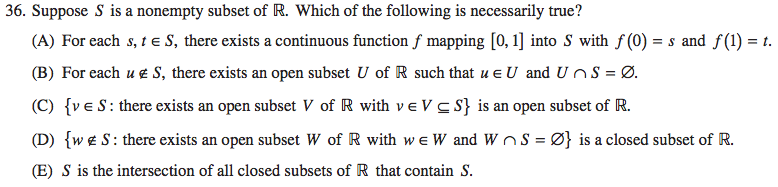
\includegraphics[scale=0.65]{1268_36}
%
%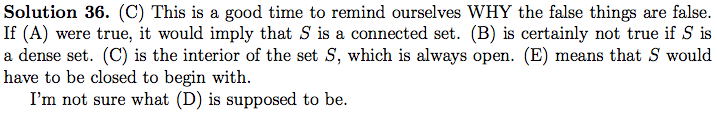
\includegraphics[scale=0.65]{1268_36s}

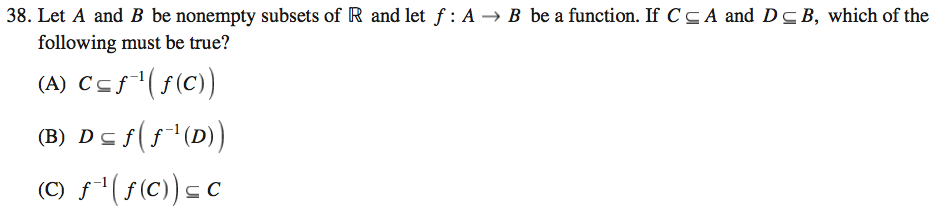
\includegraphics[scale=0.5]{0568_38}

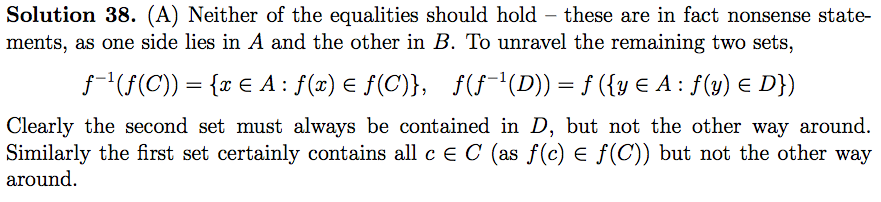
\includegraphics[scale=0.5]{0568_38s}

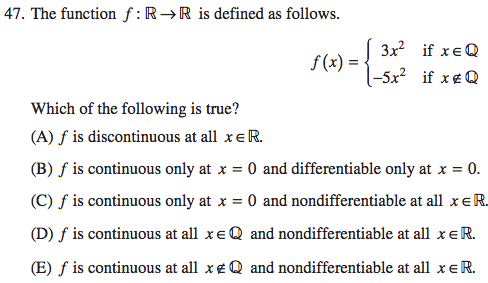
\includegraphics[scale=0.65]{1268_47}

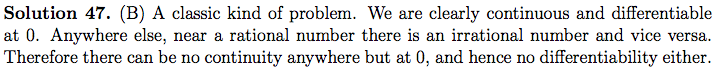
\includegraphics[scale=0.65]{1268_47s}

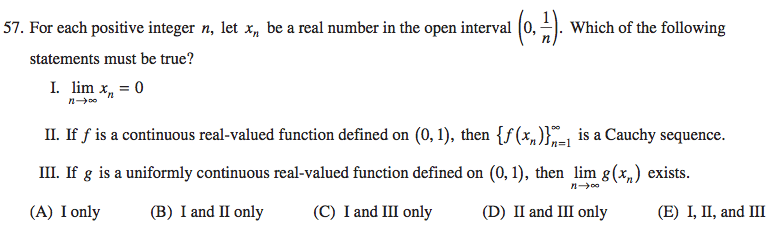
\includegraphics[scale=0.65]{1268_57}

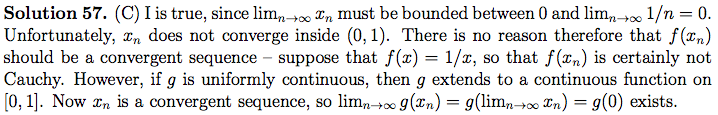
\includegraphics[scale=0.65]{1268_57s}

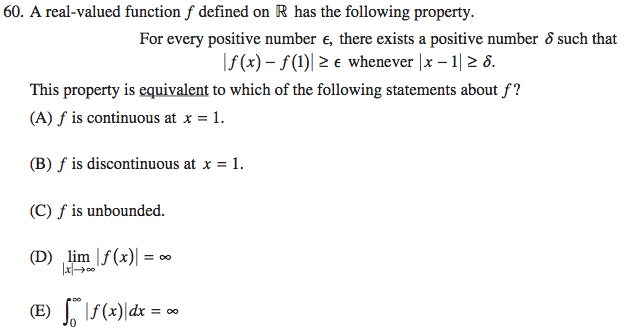
\includegraphics[scale=0.65]{1268_60}

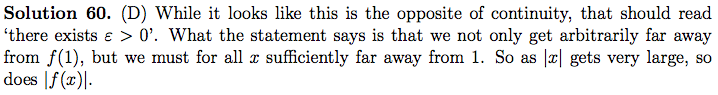
\includegraphics[scale=0.65]{1268_60s}

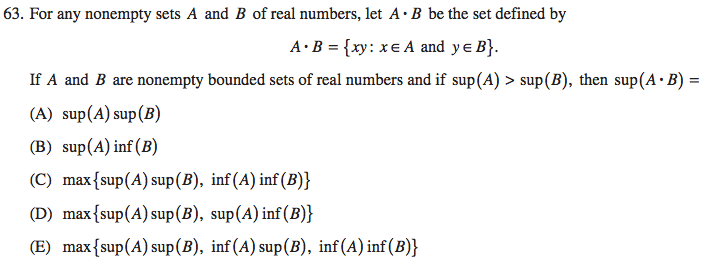
\includegraphics[scale=0.65]{1268_63}

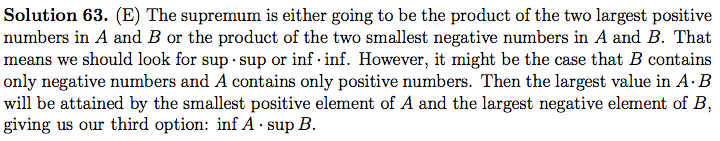
\includegraphics[scale=0.65]{1268_63s}

%
%
%
%
%
%
%
%

%\bibliographystyle{abbrvnat}
%\bibliography{mybib2fin}
%
%\end{document}